\chapter{A ROM Based on the Grey LOQD Equations and Proper Orthogonal Decomposition of QD Factors and Energy Density Spectrum}
\label{chap-four}

\newcommand{\amodkapebin}{\kapebin^{\tau*}}
\newcommand{\amodkaprbirn}{\kaprbirn^{\tau*}}
\newcommand{\amodkapgirn}{\kapgirn^{\tau*}}
\newcommand{\amodkapgirrn}{\kapgirrn^{\tau*}}

\newcommand{\aetailnp}{\eta_{i-\frac{1}{2},n}^{+*}}
\newcommand{\aetailnm}{\eta_{i-\frac{1}{2},n}^{-*}}
\newcommand{\aetairnp}{\eta_{i+\frac{1}{2},n}^{+*}}
\newcommand{\aetairnm}{\eta_{i+\frac{1}{2},n}^{-*}}

This chapter develops a ROM for solving TRT problems based on the effective grey problem described in Sec. \ref{eff_gr_prb}. The POD (Sec. \ref{sec:pod}) is used to approximate the group QD factors and the solution of the multigroup LOQD system. Section \ref{sec:pod-qd} formulates the ROM, henceforth referred to as the GLOQD-POD ROM. Sections \ref{reduced_eg} and \ref{bb_cor} analyze the POD of the group radiation energy densities and formulate a method of correcting those approximate radiation energy densities. Section \ref{sec:gloqd-pod_res} describes the numerical results of this ROM.

%=================================================================================
% POD-BASED REPRESENTATION  OF SPECTRUM
%=================================================================================
\section{Formulation of the GLOQD-POD ROM} \label{sec:pod-gqd} 
	We apply the POD methodology on the discrete set of group energy densities $E_g(x,t)$. The discrete group energy densities are defined on grids of energy, space and time, and the POD is applied to each energy group separately to obtain approximations over space and time \cite{dya-jcp-2019}. The same procedure as applied to the group QD factors (Ch. \ref{chap-three}) is followed by forming $N_g$ group-wise matrices $\bA^{E}_g \in \real^{\chi,\tau}$ where each matrix holds the set of group $g$ energy densities. $\chi$ and $\tau$ are the number of discrete spatial and temporal nodes respectively. Each column in $\bA^E_g$ contains the spatial vector of the group energy densities at a separate instant of time, ordered chronologically. The SVD  is applied to each $\bA^E_g$ to cast in the form of \eqn{svd_form}, $\bA^E_g = \bU_g\bSig_g\bV_g^T$ where $\bU_g \in \real^{\chi,k}$, $\bSig_g \in \real^{k,k}$, $\bV_g \in \real^{\tau,k}$, and $k = \min\pr{\chi,\tau}$. The reduced rank approximation of each group energy density matrix is given as $\bA^{E*}_g  = \bU^*_g\bSig^*_g\pr{\bV^{*}_g}^T $ where $\bU^*_g \in \real^{\chi,r_g}$, $\bSig^*_g \in \real^{r_g,r_g}$, $\bV^{*}_g \in \real^{\tau,r_g}$. $r_g$ is the reduced rank determined by $\varepsilon_\sigma$ (Eq. \ref{cutoff_eps}), and the $\gamma_n$ of the singular values used is calculated as $\gamma_{r_g}$ (Eq. \ref{worth_gam}).
	
	\ind Given approximate QD factors $f_g^*$ and radiation energy densities $E_g^*$ calculated with a low-rank POD, a set of corresponding group radiation fluxes at each instant of time $\bFg^*\pr{x,t}$ can be calculated with the multigroup MLOQD-POD system \eqref{mqd_sys}. This defines group radiation fluxes according to the group first moment QD equation (Eq. \ref{mqd_2}) and the reduced rank group radiation energy densities. The quantities required for the effective grey problem are calculated with the approximate multigroup solution and group QD factors. The approximate grey QD factors are calculated as
	\begin{align}
		\bar{f}^*\pr{x,t} = \frac{ \sum_{g=1}^{N_g}\fg^*\pr{x,t}\eg^*\pr{x,t} }{ \sum_{g=1}^{N_g}\eg^*\pr{x,t} },
	\end{align}
	
	where $\fg^*$ and $\eg^*$ are the approximate group QD factors and radiation energy densities obtained from the low-rank POD, namely, $\bA^{f*}_g$ and $\bA^{E*}_g$. Similarly we define two approximate grey opacities \eqref{grey_opacities}
	\begin{gather}
		\kapeb^*\pr{T} = \frac{ \sum_{g=1}^{N_g}\kapg\pr{T}\eg^*\pr{x,t} }{ \sum_{g=1}^{N_g}\eg^*\pr{x,t} }, \\[5pt]
		\kaprb^*\pr{T} = \frac{ \sum_{g=1}^{N_g}\kapg\pr{T}\abs{\bFg^*\pr{x,t}} }{ \sum_{g=1}^{N_g}\abs{\bFg^*\pr{x,t}} },
	\end{gather}
	
	and the compensation factor \eqref{eta_comp} is calculated as
	\begin{equation}
		\eta^*\pr{x,t} = \frac{ \sum_{g=1}^{N_g}\brk{\pr{\kapg\pr{T} - \kaprb^*\pr{T}}\bFg^*\pr{x,t}} }{ \sum_{g=1}^{N_g}\eg^*\pr{x,t} }.
	\end{equation}
	
	The GLOQD-POD ROM is characterized by the resulting GLOQD and MEB equations using approximate quantities
	\begin{subequations}
		\begin{gather}
			\dt{\eb\pr{x,t}} + \grad\cdot\bFb\pr{x,t} + c\kapeb^*\pr{T}\eb\pr{x,t} = c\kapbb^*\pr{T}\ar T^4 \label{glqd_pod_zero} \\
			\frac{1}{c}\dt{\bFb\pr{x,t}} + c\grad\cdot\pr{\fb^*\pr{x,t}\eb\pr{x,t}} + \kaprb^*\pr{T}\bFb\pr{x,t} + \eta^*\pr{x,t}\eb\pr{x,t}= 0 \label{glqd_pod_first} \\
			\dt{\varepsilon\pr{T}} = c\kapeb^*\pr{T}\eb\pr{x,t} - c\kapbb^*\pr{T}\ar T^4. \label{EB_gpod}
		\end{gather}
		\label{glqd_pod_eqs}
	\end{subequations}

	\iffalse
	In discrete space the GLOQD-POD ROM is
	\begin{subequations}
		\begin{gather}
			\Fbirn - \Fbiln + c\delxi\amodkapebin\pr{T}\ebin = c\kapbbin^*\pr{T}\ar T^4_{i,n} + \frac{\ebinl}{\deltn}
		\end{gather}
		\vspace*{-1.2cm}
		\begin{multline}
			c\pr{\fbirrn^*\ebirrn - \fbin^*\ebin} + \delxir\amodkaprbirn\pr{T}\Fbirn \\+ \pr{\aetairnp\ebirrn - \aetairnm\ebin} = \delxir\frac{\Fbirnl}{c\deltn}
		\end{multline}
		\vspace*{-.9cm}
		\begin{gather}
			\frac{\varepsilon_{i,n}\pr{T} - \varepsilon_{i,n-1}\pr{T}}{\delt_n} = c\kapebin^*\ebin - c\ar\kapbbin^*\tin^4\\
			i = 1,\dots,I, \ n = 1,\dots,N_n \nn
		\end{gather}
	\end{subequations}
	\fi
	
	
	\iffalse
	 as the elements of the $n^{\text{th}}$ column of the low-rank SVD of $\bA_g^f$ and $\bA_g^E$ respectively
	\begin{equation}
		\fgin^* = \Big(a^{f*}_{i,n}\Big)_g, \ \
		\egin^* = \Big(a^{E*}_{i,n}\Big)_g,
	\end{equation}
	
	with $\pr{a^{f*}_{i,n}}_g$ and $\pr{a^{E*}_{i,n}}_g$ as the $\pr{i,n}$ element of the matrices $\bA_g^{f*}$ and $\bA_g^{E*}$.
	\fi
	 
	
	\iffalse
	The discrete grey opacities are
	\begin{subequations}
		\begin{gather}
			\kapebin^*\pr{T} = \frac{ \sum_{g=1}^{N_g}\kapgin\pr{T}\egin^* }{ \sum_{g=1}^{N_g}\egin^* } \\[5pt]
			\kapbbin\pr{T} = \frac{ \sum_{g=1}^{N_g}\kapgin\pr{T}\Bgin\pr{T} }{ \sum_{g=1}^{N_g}\Bgin\pr{T} } \\[5pt]
			\kaprbirn^*\pr{T} = \frac{ \sum_{g=1}^{N_g}\kapgirn\pr{T}\abs{\Fgirn^*} }{ \sum_{g=1}^{N_g}\abs{\Fgirn^*} },
		\end{gather}
	\end{subequations}
	
	and the modified opacities are
	\begin{subequations}
	\begin{gather}
		\amodkapebin\pr{T} = \kapebin^*\pr{T} + \frac{1}{c\deltn}, \\
		\amodkaprbirn\pr{T} = \kaprbirn^*\pr{T} + \frac{1}{c\deltn}.
	\end{gather}
	\end{subequations}
	
	The discrete compensation term is
	\begin{subequations}
		\begin{align}
			&\etairn^* = \sum_{g=1}^{N_g} \brk{\pr{\kapgirn - \kaprbirn^*}\Fgirn^*}\\
			&\aetairnp = \left\{ \begin{array}{ll}
						\frac{\etairn^*}{\sum_{g=1}^{N_g} \egirrn^*} & \etairn^*>0\\
						0 & \etairn^*<0
					\end{array} \right.\\
			&\aetairnm = \left\{ \begin{array}{ll}
						0 & \etairn^*>0\\
						\frac{-\etairn^*}{\sum_{g=1}^{N_g} \egin^*} & \etairn^*<0
					\end{array} \right.
		\end{align}
	\end{subequations}
	\fi
	
	In discrete space this ROM is given by the GLOQD Eqs. \eqref{gqd_sys_disc} and MEB Eq. \eqref{ebdisc2} with the POD quantities described in this section. The group cell average QD factors and radiation energy densities at each instant of time $\pr{n}$ are defined as described for $\fgin^*$ in Sec. \ref{sec:pod-qd}. The radiation flux $\Fgirn^*$ is calculated with the MLOQD-POD system \eqref{mlqd_pod_eqs} given $\fgin^*$ and $\egin^*$. Note that the derived ROM does not solve the RT or MLOQD equations except to update the group radiation fluxes. Algorithm \ref{alg:glqd_rom_alg} shows the iterative scheme for the GLOQD-POD ROM for TRT problems.
	
	\begin{algorithm}[ht!]
		\SetAlgoLined
		\While{$t^n<t^{\text{end}}$}{
			$n=n+1$\\
			$T^{\pr{0}} = T^{n-1}$\\
			$\bfg^* \leftarrow \bA^{f*}_g$, \ \ $\eg^* \leftarrow \bA^{E*}_g$\\
			%Calculate $\bFg$ from MLOQD-POD Eqs. \eqref{mlqd_pod_eqs}\\
			\While{$\norm{T^{\ell}-T^{\ell-1}} > \tilde{\epsilon}_1\norm{T^{\ell}} + \tilde{\epsilon}_2, \ \ \norm{\eb^{\ell}-\eb^{\ell-1}} > \tilde{\epsilon}_1\norm{\eb^{\ell}} + \tilde{\epsilon}_2 $}{
				$\ell=\ell+1$
				Update opacities $\kapg\pr{T^{\ell}}$\\
				Update group radiation fluxes $\bFg^*$ with MLOQD-POD Eqs. \eqref{mlqd_pod_eqs}\\
				Compute grey quantities $\kapeb^{*,\ell}$, $\kapbb^{\ell}$, $\kaprb^{*,\ell}$, $\bfb^{*,\ell}$, $\etab^{*,\ell}$\\
				Solve coupled GLOQD-POD and MEB Eqs. \eqref{glqd_pod_eqs} for $\eb^{\ell}$, $\bFb^{\ell}$, $T^{\ell}$
			}
			$T^n \leftarrow T^\ell$
		}
		\caption{Nonlinear QD Iterative Scheme for the GLOQD-POD ROM using reduced rank databases of group QD factors $\bA^{f*}_g$ and group radiation energy densities $\bA^{E*}_g$ \label{alg:glqd_rom_alg}}
	\end{algorithm}
	
%=================================================================================
% Numerical Results
%=================================================================================
%\section{Test Problem Formulation} \label{sec:gpod_test} 
%	In this section we present computational results for the same 1D F-C test as described for section \ref{sec:mpod_test}. Given the same test conditions, the analysis for the reduced rank QD factors is equivalent to that shown in section \ref{sec:reduced_qdf}.

\section{Low-Rank Approximation of Group Energy Densities} \label{reduced_eg}
	%In this section computational results are presented for the same 1D F-C test as described for Sec. \ref{sec:mpod_test}. Given the same test conditions, the analysis for the reduced rank group QD factors is equivalent to that shown in section \ref{sec:reduced_qdf}.
	
	Analysis of reduced rank forms of the group QD factors is given in Ch. \ref{chap-three}. Fig. \ref{fig:Eg_sval_summary} displays the normalized magnitudes and $1-\gamma_n$ of the singular values of $\bA^E_g$ for each energy group. Since the test problem has 60 spatial cells the vector of cell-average group radiation energy densities in space has 62 values including 2 boundary values. When $\varepsilon_\sigma=10^{-12}$, the full-rank SVD is used. The low energy groups $g=\pr{1,2,3,4}$ require the highest ranks for the shown values of $\varepsilon_\sigma$ and the middle groups require the lowest ranks. The singular values normalized to the largest singular value for all energy groups are shown in Fig. \ref{subfig:EG_Svals_grey}, where each energy group has a horizontal plateau of values that starts at roughly $r=30$. These plateaus decrease in magnitude as $g$ is increased. Note that there is a large gap between the observed plateaus of groups 1,2,3 and the latter energy groups. The same behavior is shown for the values of $1-\gamma_n$ for each energy group in Fig. \ref{subfig:inv_worths_Eg_grey}. The higher energy groups reach numerically zero ($10^{-16}$) for $1-\gamma_n$ at roughly the same point where the singular value plateau occurs. The large gap between low energy groups and middle to high energy groups implies low energy groups to be the most difficult to approximate with low rank forms. Table \ref{tab:gqd_sigtab} displays the rank of approximation $(r_g)$ involved per energy group at different values of  $\varepsilon_\sigma$.
	
	%=================================================================================
	% SINGULAR VALUE FIGS
	\begin{figure}[ht!]
		\centering
		\subfloat[Normalized singular values of $\bA^E_g$ (group radiation energy density database matrices) \label{subfig:EG_Svals_grey}]{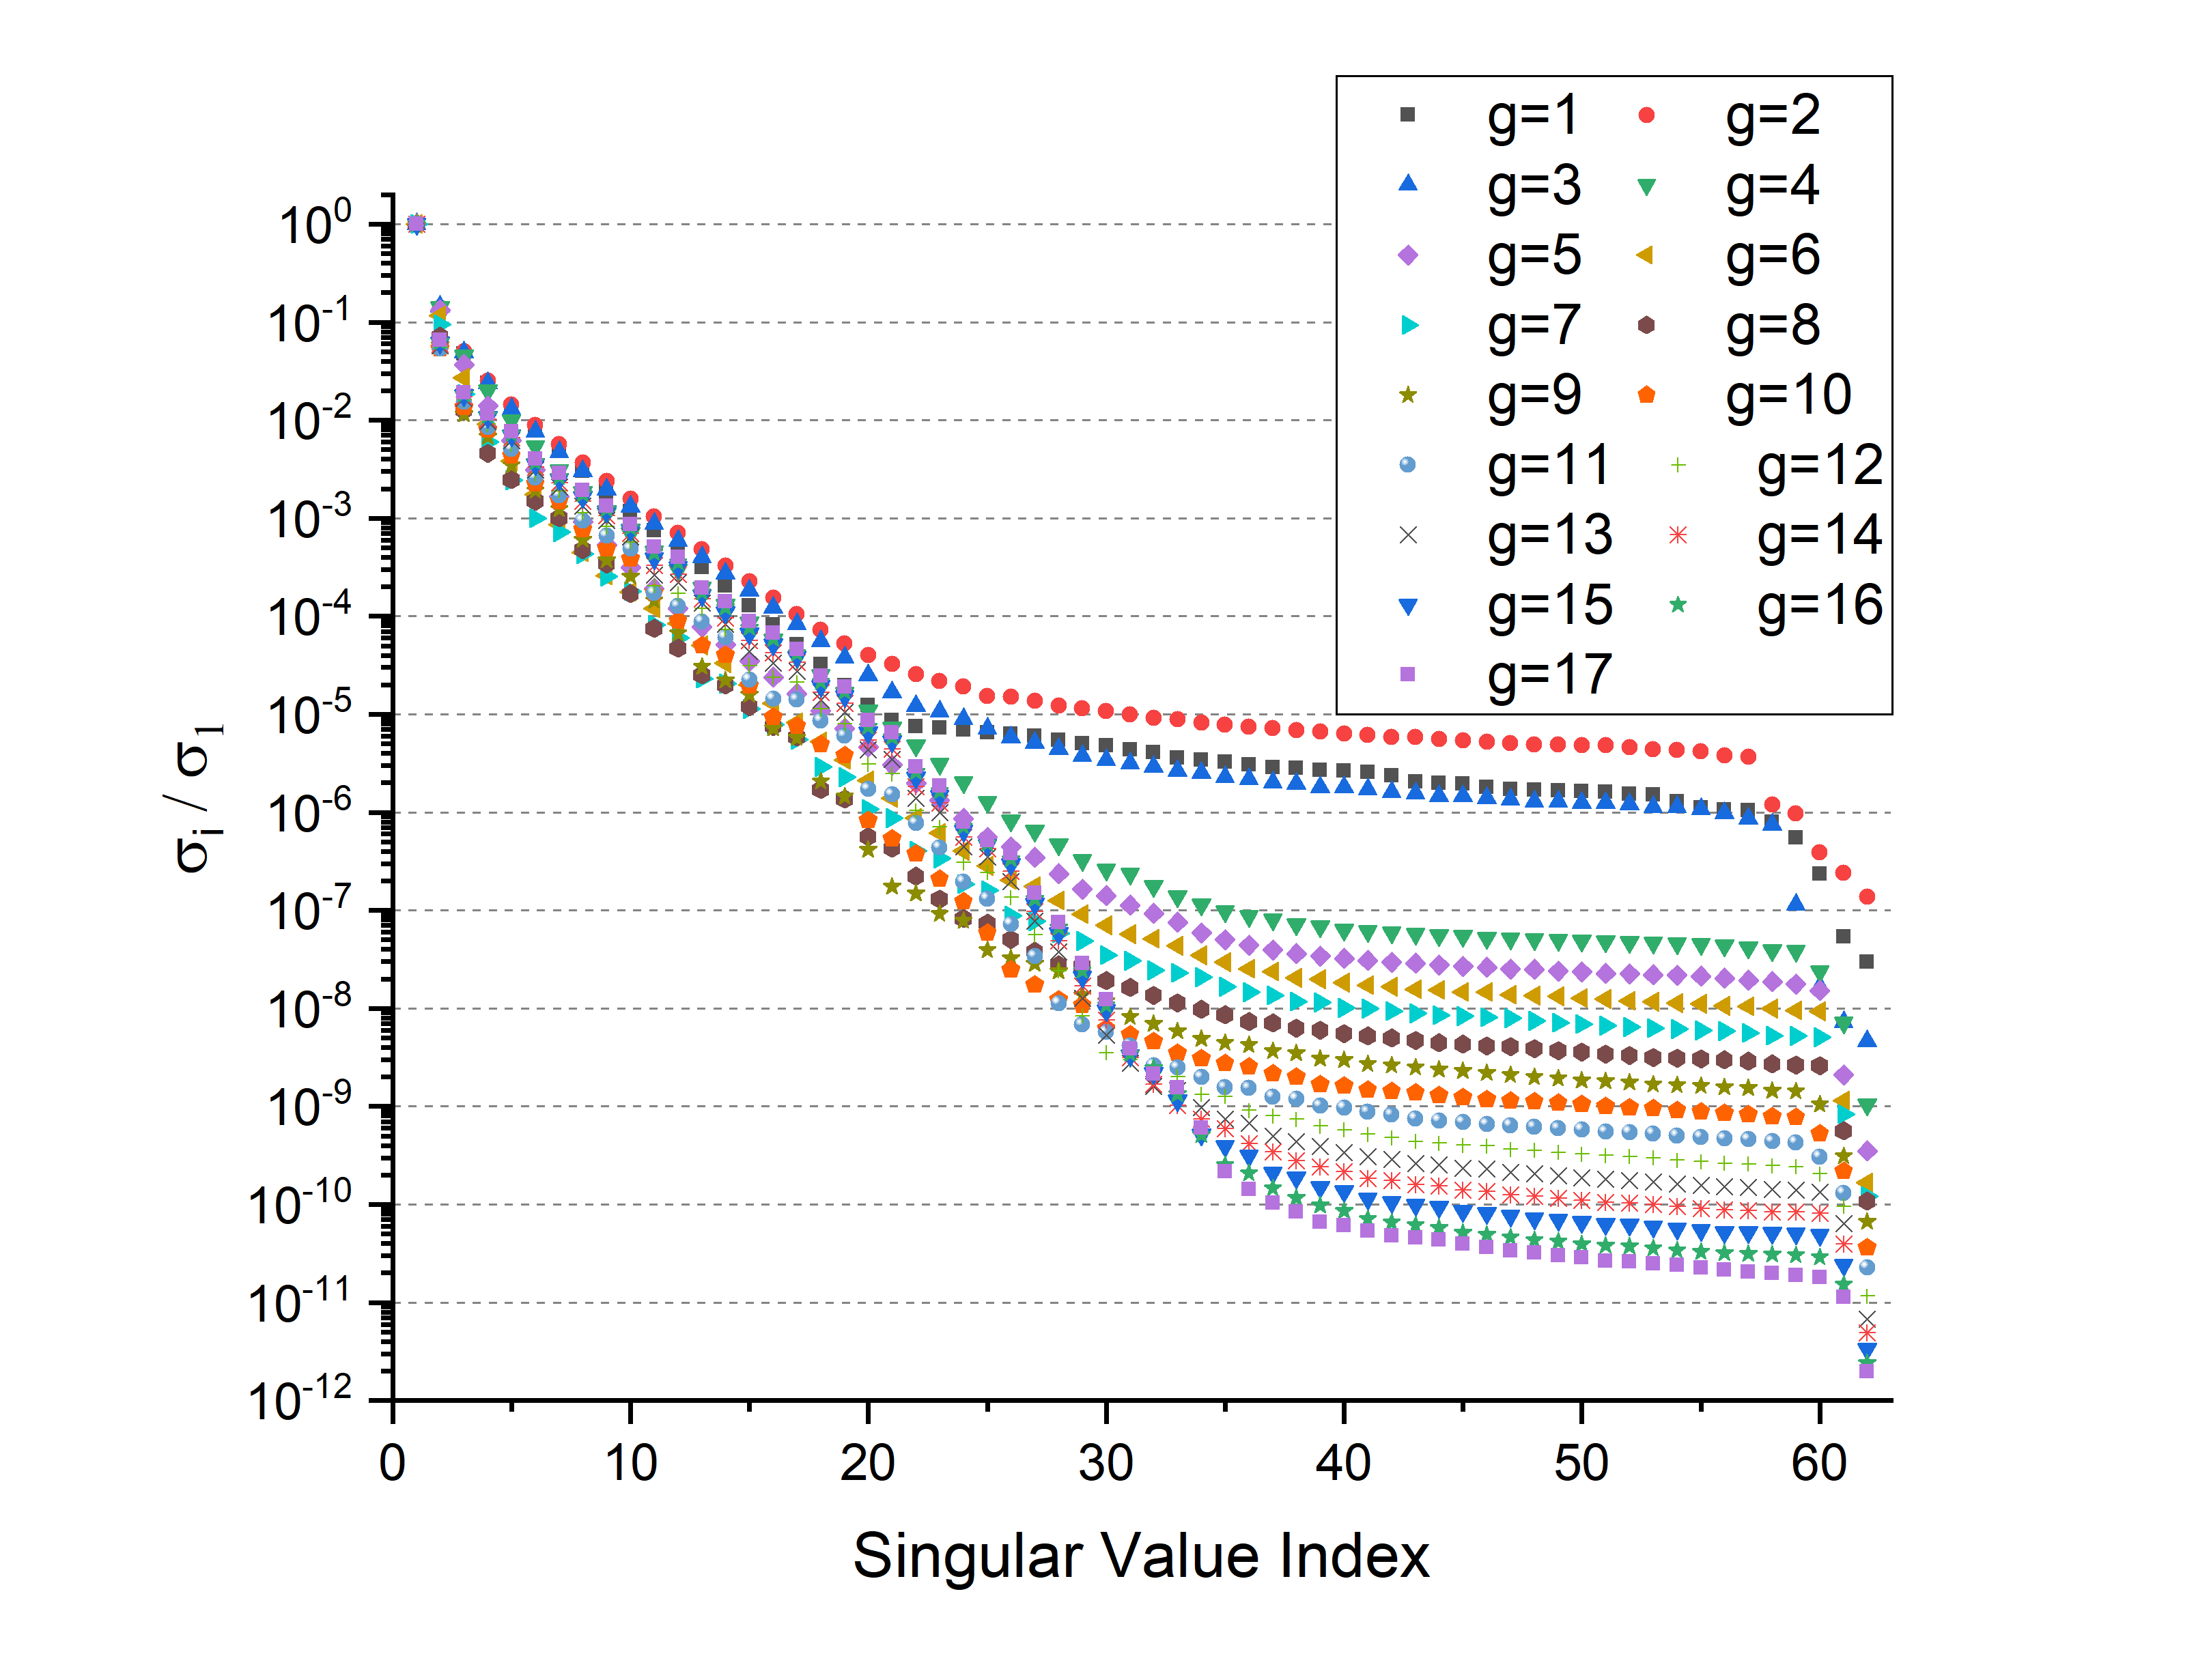
\includegraphics[width=0.5\textwidth]{Eg_normalized_svals.png}} \hspace*{.5cm}
		\subfloat[$1-\gamma_n$ for $\bA^E_g$ (group radiation energy density database matrices) \label{subfig:inv_worths_Eg_grey}]{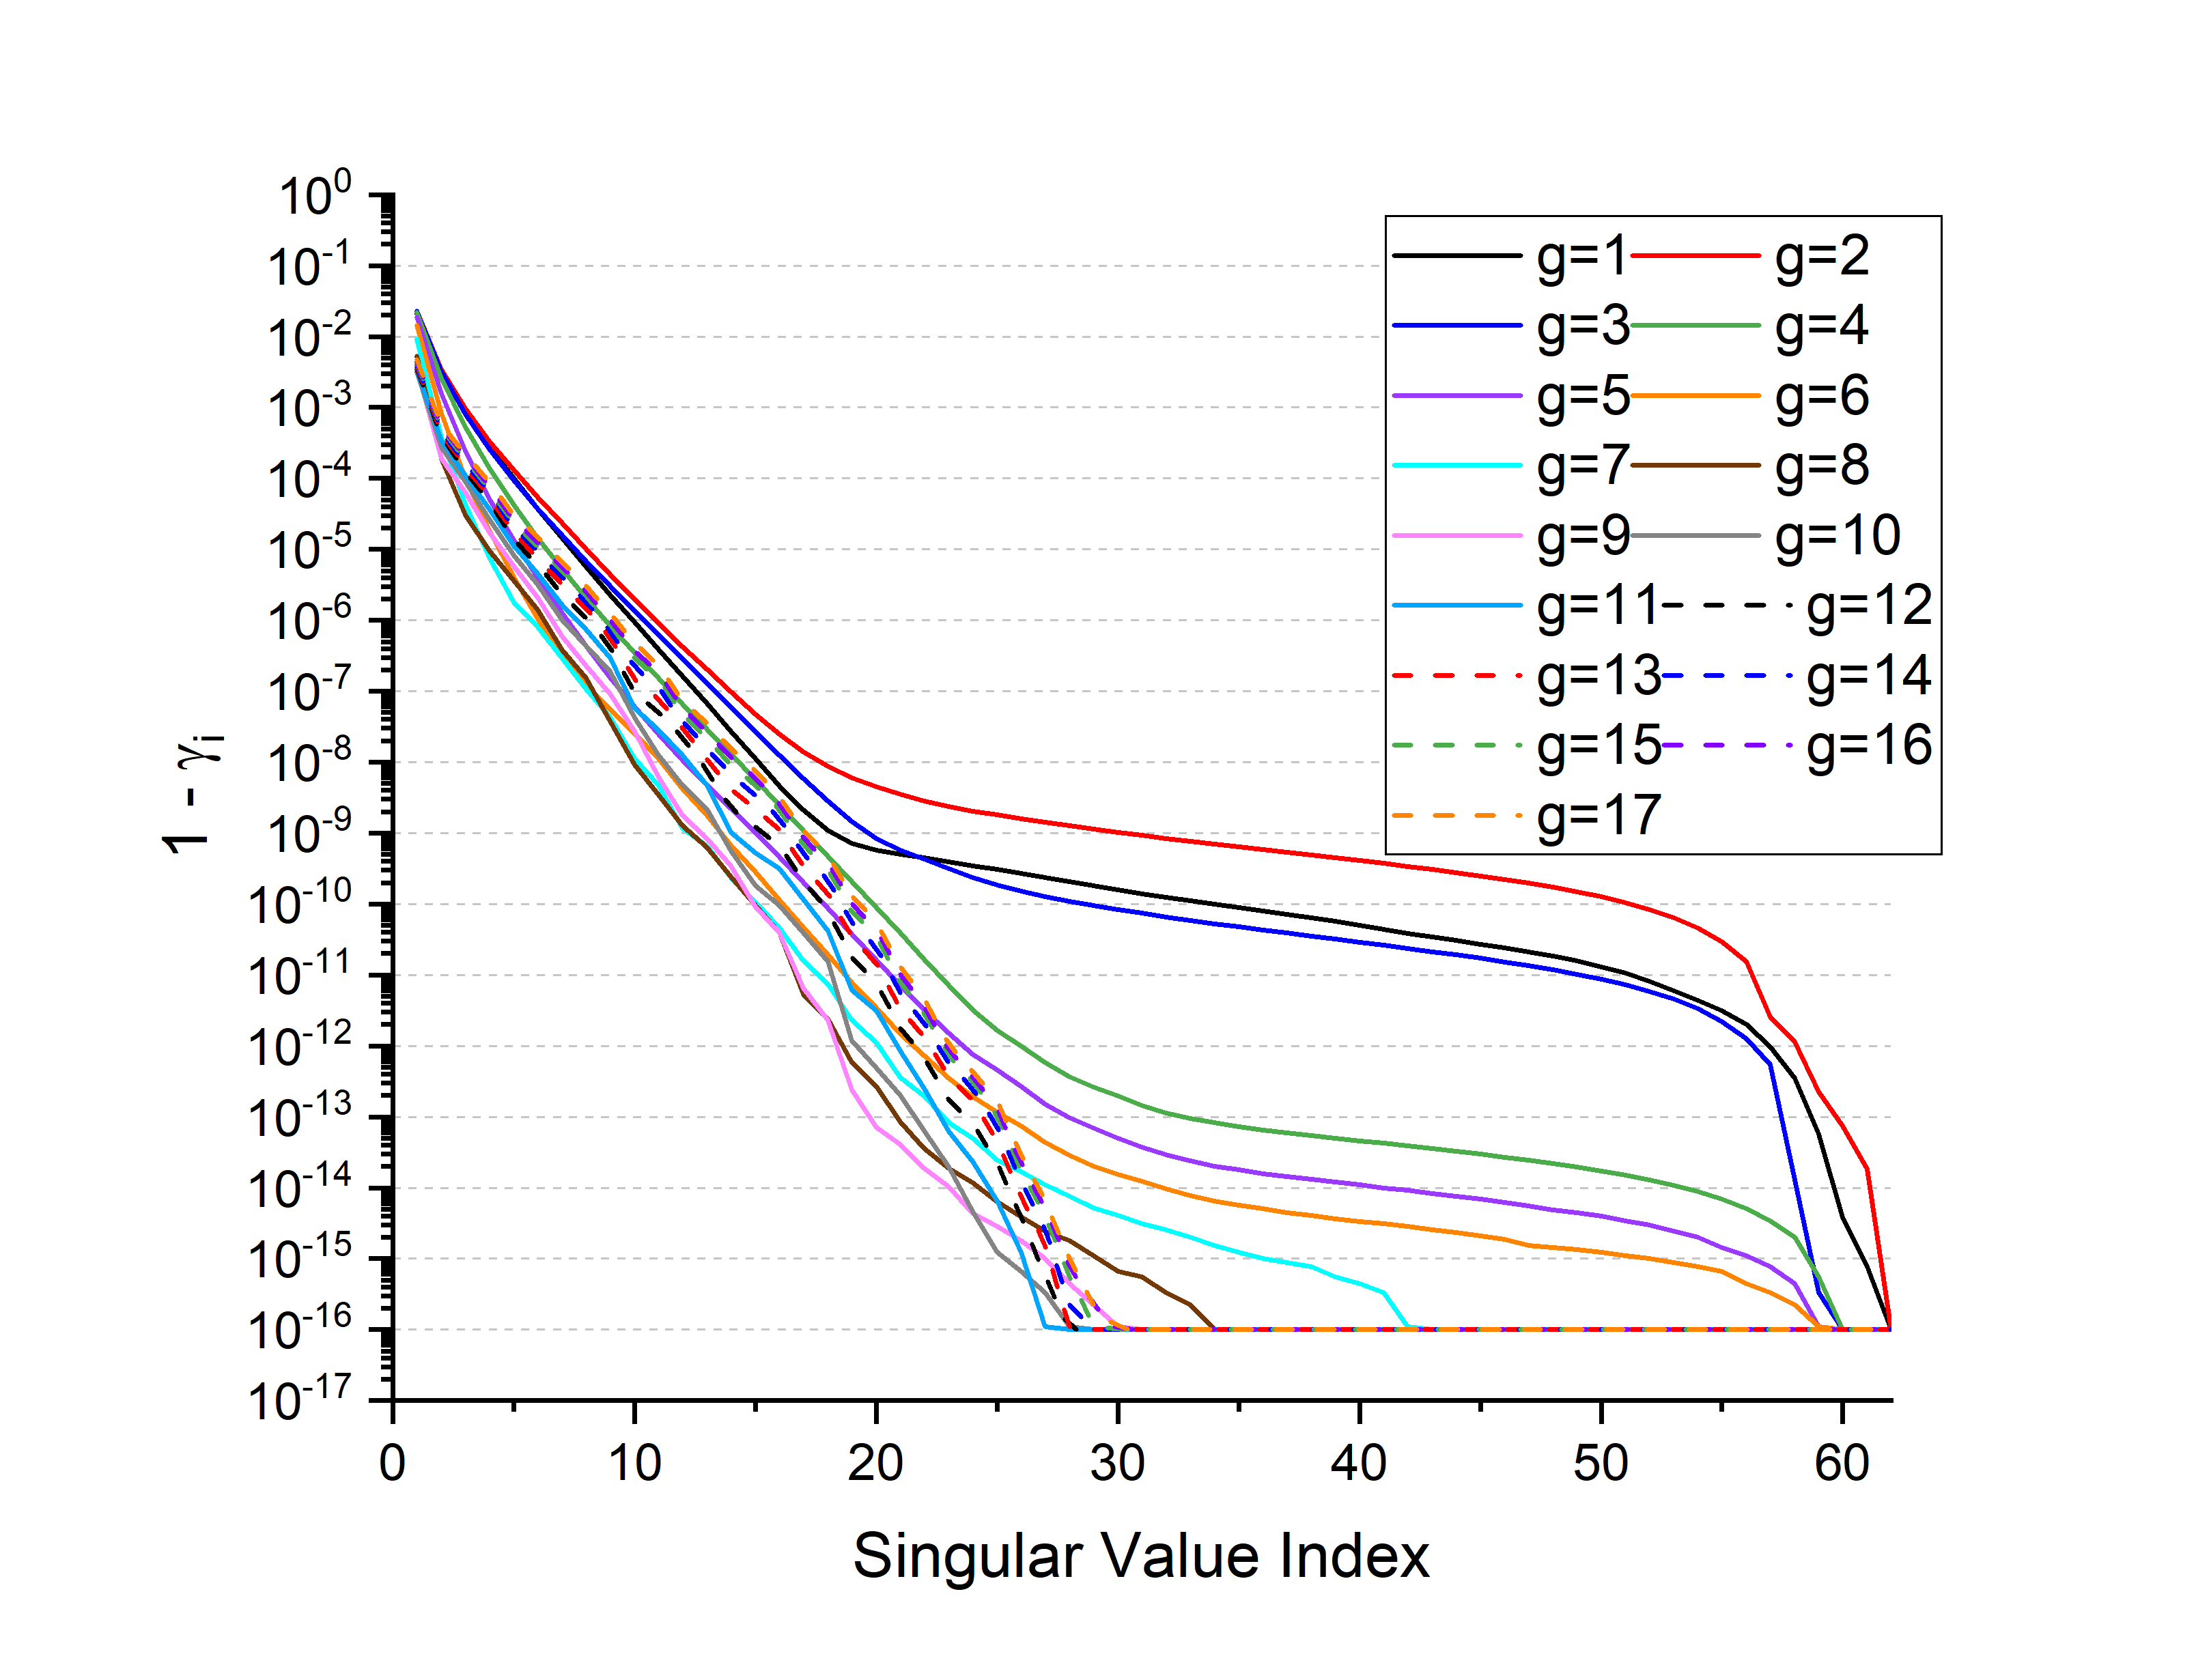
\includegraphics[width=0.5\textwidth]{inv_worths_Eg_grey.png}}
		\caption{\label{fig:Eg_sval_summary}
			Group radiation energy density normalized singular values and $1-\gamma_n$}
	\end{figure}
	
	%=================================================================================
	% SINGULAR VALUE TABLE
	\begin{table}[ht!]
		\caption{	\label{tab:gqd_sigtab} The rank of approximation $(r_g)$ of $E_g$ in each energy group for decreasing values of $\varepsilon_\sigma$}
		\begin{tabular}{|c||c|c|c|c|c|c|c|c|c|c|c|c|c|c|c|c|c|}	
			\hline
			$\varepsilon_\sigma \backslash  \ g$ & 1 & 2 & 3 & 4 & 5 & 6 & 7 & 8 & 9 & 10 & 11 & 12 & 13 & 14 & 15 & 16 & 17 \\
			\hline
			\hline
			$10^{-1}$ & 2  &  2 & 2  & 2  & 2  & 2  &  1 & 1 &  1 &   1 & 1 &  1 &  1 & 1 &  1 &  1 & 1 \\ \hline
			$10^{-2}$ & 5 & 5 & 5 & 4 & 4 & 3 & 3 & 3 & 3 & 3 & 3 & 3 & 3 & 4 & 4 & 4 & 4\\ \hline
			$10^{-3}$ & 10 & 11 & 10 & 9 & 7 & 6 & 5 & 7 & 7 & 7 & 7 & 8 & 8 & 9 & 9 & 9 & 9\\ \hline
			$10^{-4}$ & 15 & 17 & 16 & 14 & 12 & 11 & 10 & 10 & 11 & 11 & 12 & 13 & 13 & 13 & 14 & 14 & 14\\ \hline
			$10^{-12}$ & 62 & 62 & 62 & 62 & 62 & 62 & 62 & 62 & 62 & 62 & 62 & 62 & 62 & 62 & 62 & 62 & 62\\ \hline
		\end{tabular}
	\end{table}

	\ind Next the reduced rank forms of the group radiation energy densities are investigated. The same select energy groups $g=\pr{2,3,8}$ as considered for the group QD factors in Ch. \ref{chap-three} are used. Once again, groups 2 and 3 are representative of the most inaccurate energy groups when approximated with low rank and group 8 acts as a representative for the rest of the group radiation energy densities. Figs. \ref{fig:Eg_g2_recomps}, \ref{fig:Eg_g3_recomps} and \ref{fig:Eg_g8_recomps} show the reduced rank group radiation energy densities for groups 2, 3 and 8 respectively. Each of these figures displays the group radiation energy densities reduced to 6 different ranks $r=\pr{1,2,5,10,15,20}$. For all plots shown when $r=20$, the structure of the group radiation energy densities has converged to the reference solution to the resolution of the plot. Groups 2 and 3 display very similar structures for all shown instants of time, which differs from group 8. 
	
	\ind The group radiation energy densities for groups 2 and 3 have converged to the resolution of the plot by the $r=15$. Group 8 shows convergence to the resolution of the plot once $r=10$. The reduced rank forms for all groups are the most inaccurate when approximating energy densities of very small magnitudes. Groups 2 and 3 most easily depict this effect, with visibly oscillatory behavior at early instants of time when the energy densities have a sharp gradient near the end of the radiation wave. This is similar to the behavior of approximate group QD factors in groups with sharp gradients or discontinuities as shown in Ch. \ref{chap-three}. Some of the reduced rank forms of the group radiation energy densities become nonphysically negative due to this oscillatory structure. Most evident in Figs. \ref{subfig:Eg_g2_cut5_grey} and \ref{subfig:Eg_g3_cut5_grey}, the energy densities become largely negative for part of the spatial domain to the right of the radiation wave. This effect persists beyond the resolution of the plots and the magnitude of these negative values is simply decreased as higher rank approximations are used. 
	
	\ind The accuracy of the reduced rank form of the group energy densities is also constrained by numeric limitations. During early times some of the low energy groups have energy densities near the right boundary that are much less than $10^{-15}$ $\text{tera-erg (Terg)}$ where $\text{Terg} = 10^{12} \ \text{erg}$ are computational units. The use of such computational units is a standard and common approach in physics (and engineering) to deal with orders of magnitude of values. The rest of the energy groups display energy densities on the order of $10^{-6} \ \text{to} \ 10^{-8} \ \text{Terg}$ near the right boundary. This is expected as for early times the radiation incoming from the left boundary has not been able to propagate far into the slab of material and thus only low energy background radiation is present near the right boundary. Given that the left boundary energy density for all groups is on the order of $10 \ \text{Terg}$ or greater, the POD inaccurately recreates values of less than $10^{-16} \ \text{ergs}^*$ due to a loss of significance caused by finite-precision arithmetics. For the same reason, energy densities with values greater than $10^{-15} \ \text{Tergs}$ may only have a few digits of accuracy if near $10^{-1} \ \text{Terg}$. Thus the full rank POD is unable to recreate the exact matrix of radiation energy densities that was decomposed.

	%=================================================================================
	% Eg G2 RECOMP
	\begin{figure}[ht!]
		\centering
		\subfloat[r = 1 \label{subfig:Eg_g2_cut1_grey}]{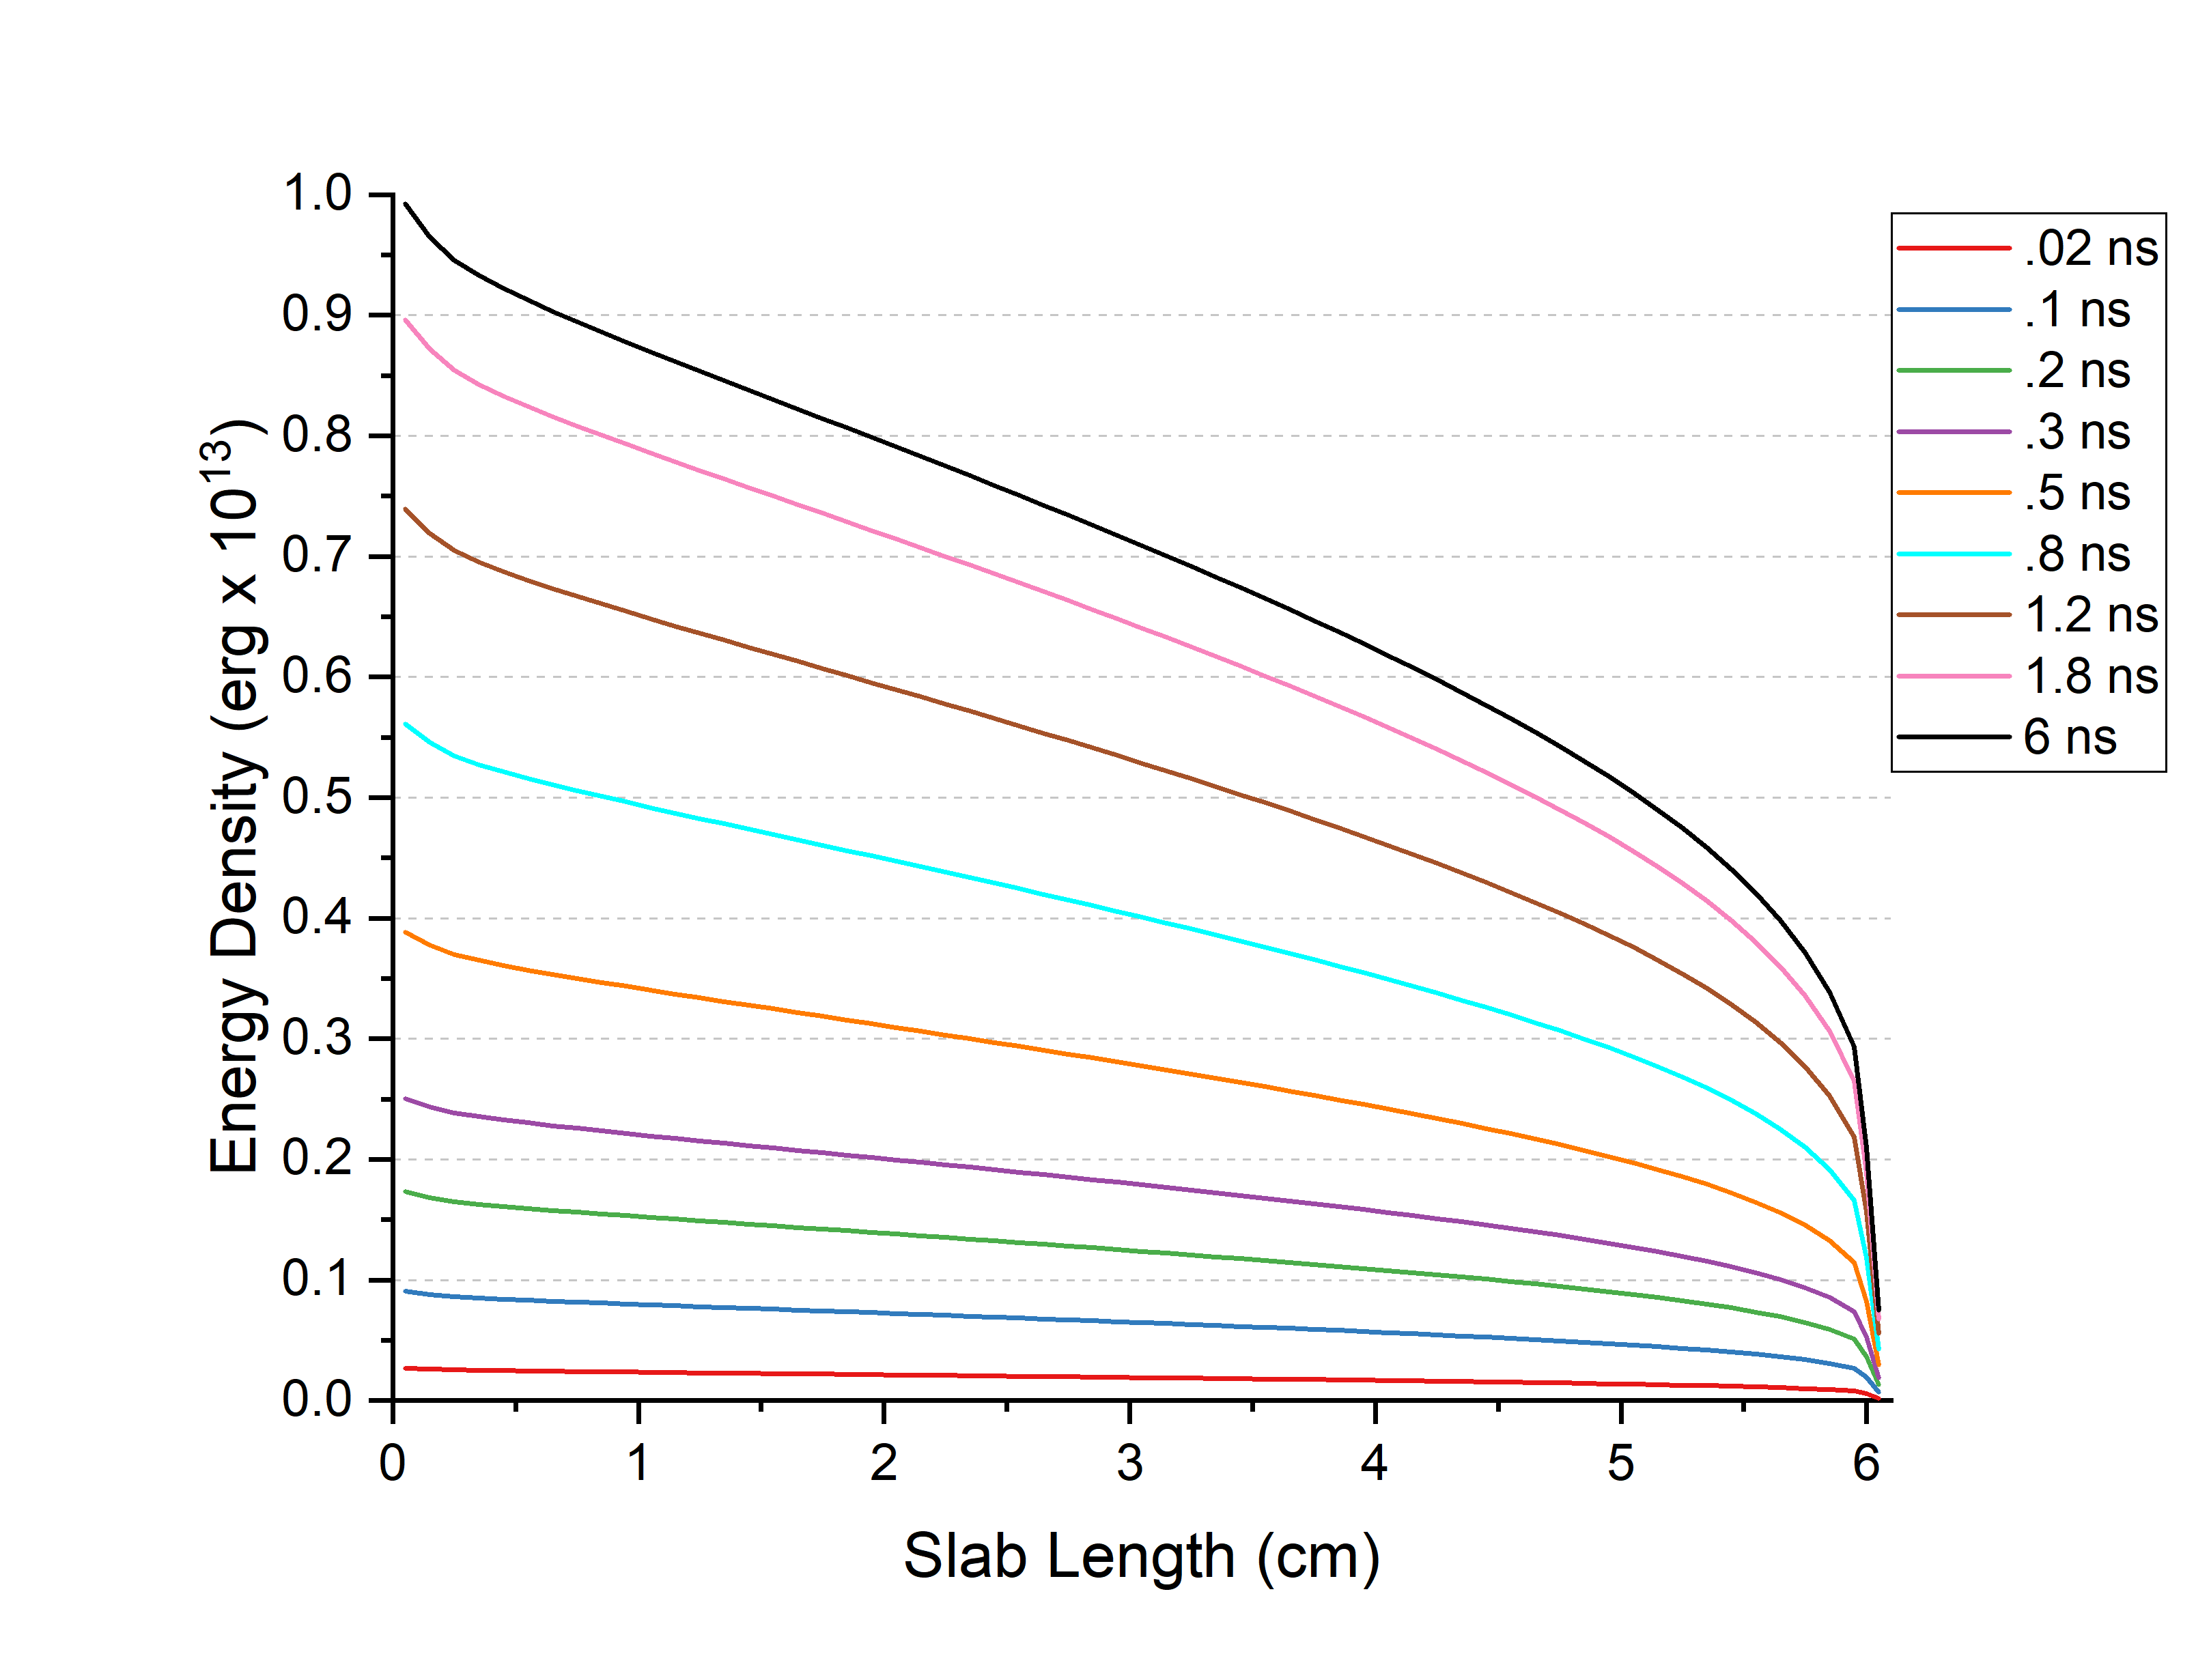
\includegraphics[width=0.5\textwidth]{Eg_g2_cut1_grey.png}}
		\subfloat[r = 2 \label{subfig:Eg_g2_cut2_grey}]{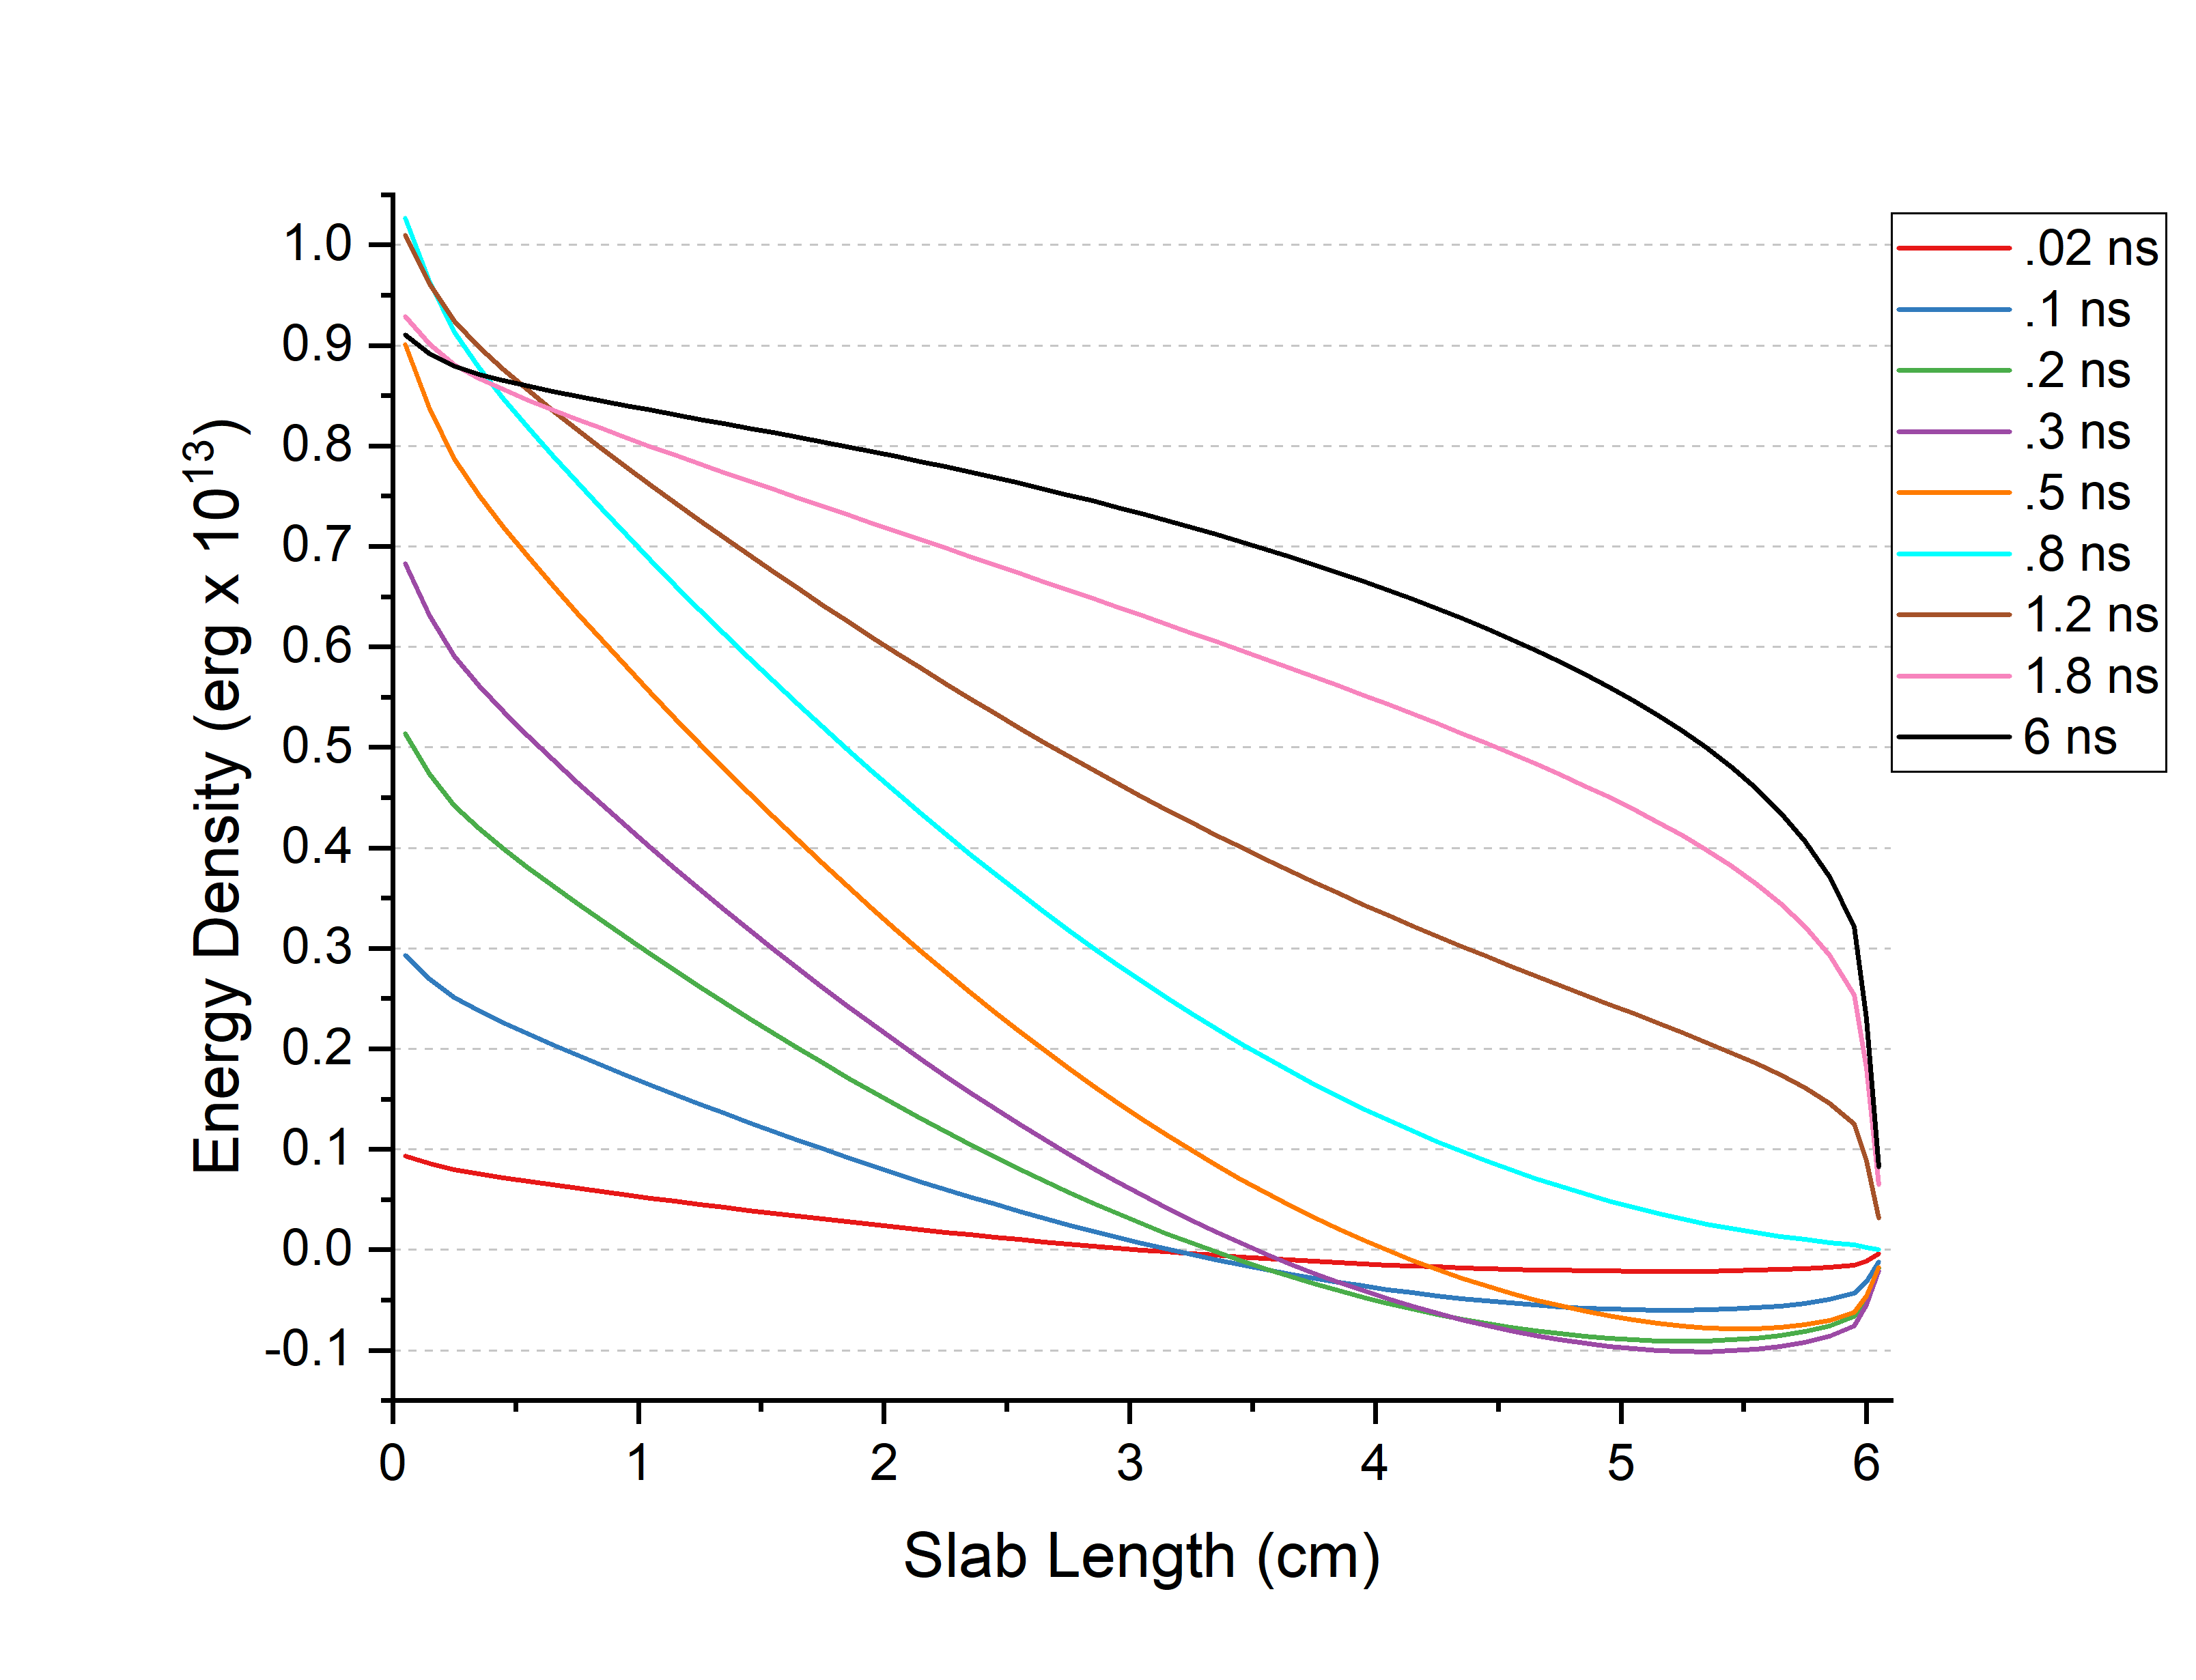
\includegraphics[width=0.5\textwidth]{Eg_g2_cut2_grey.png}}\\
		\subfloat[r = 5 \label{subfig:Eg_g2_cut5_grey}]{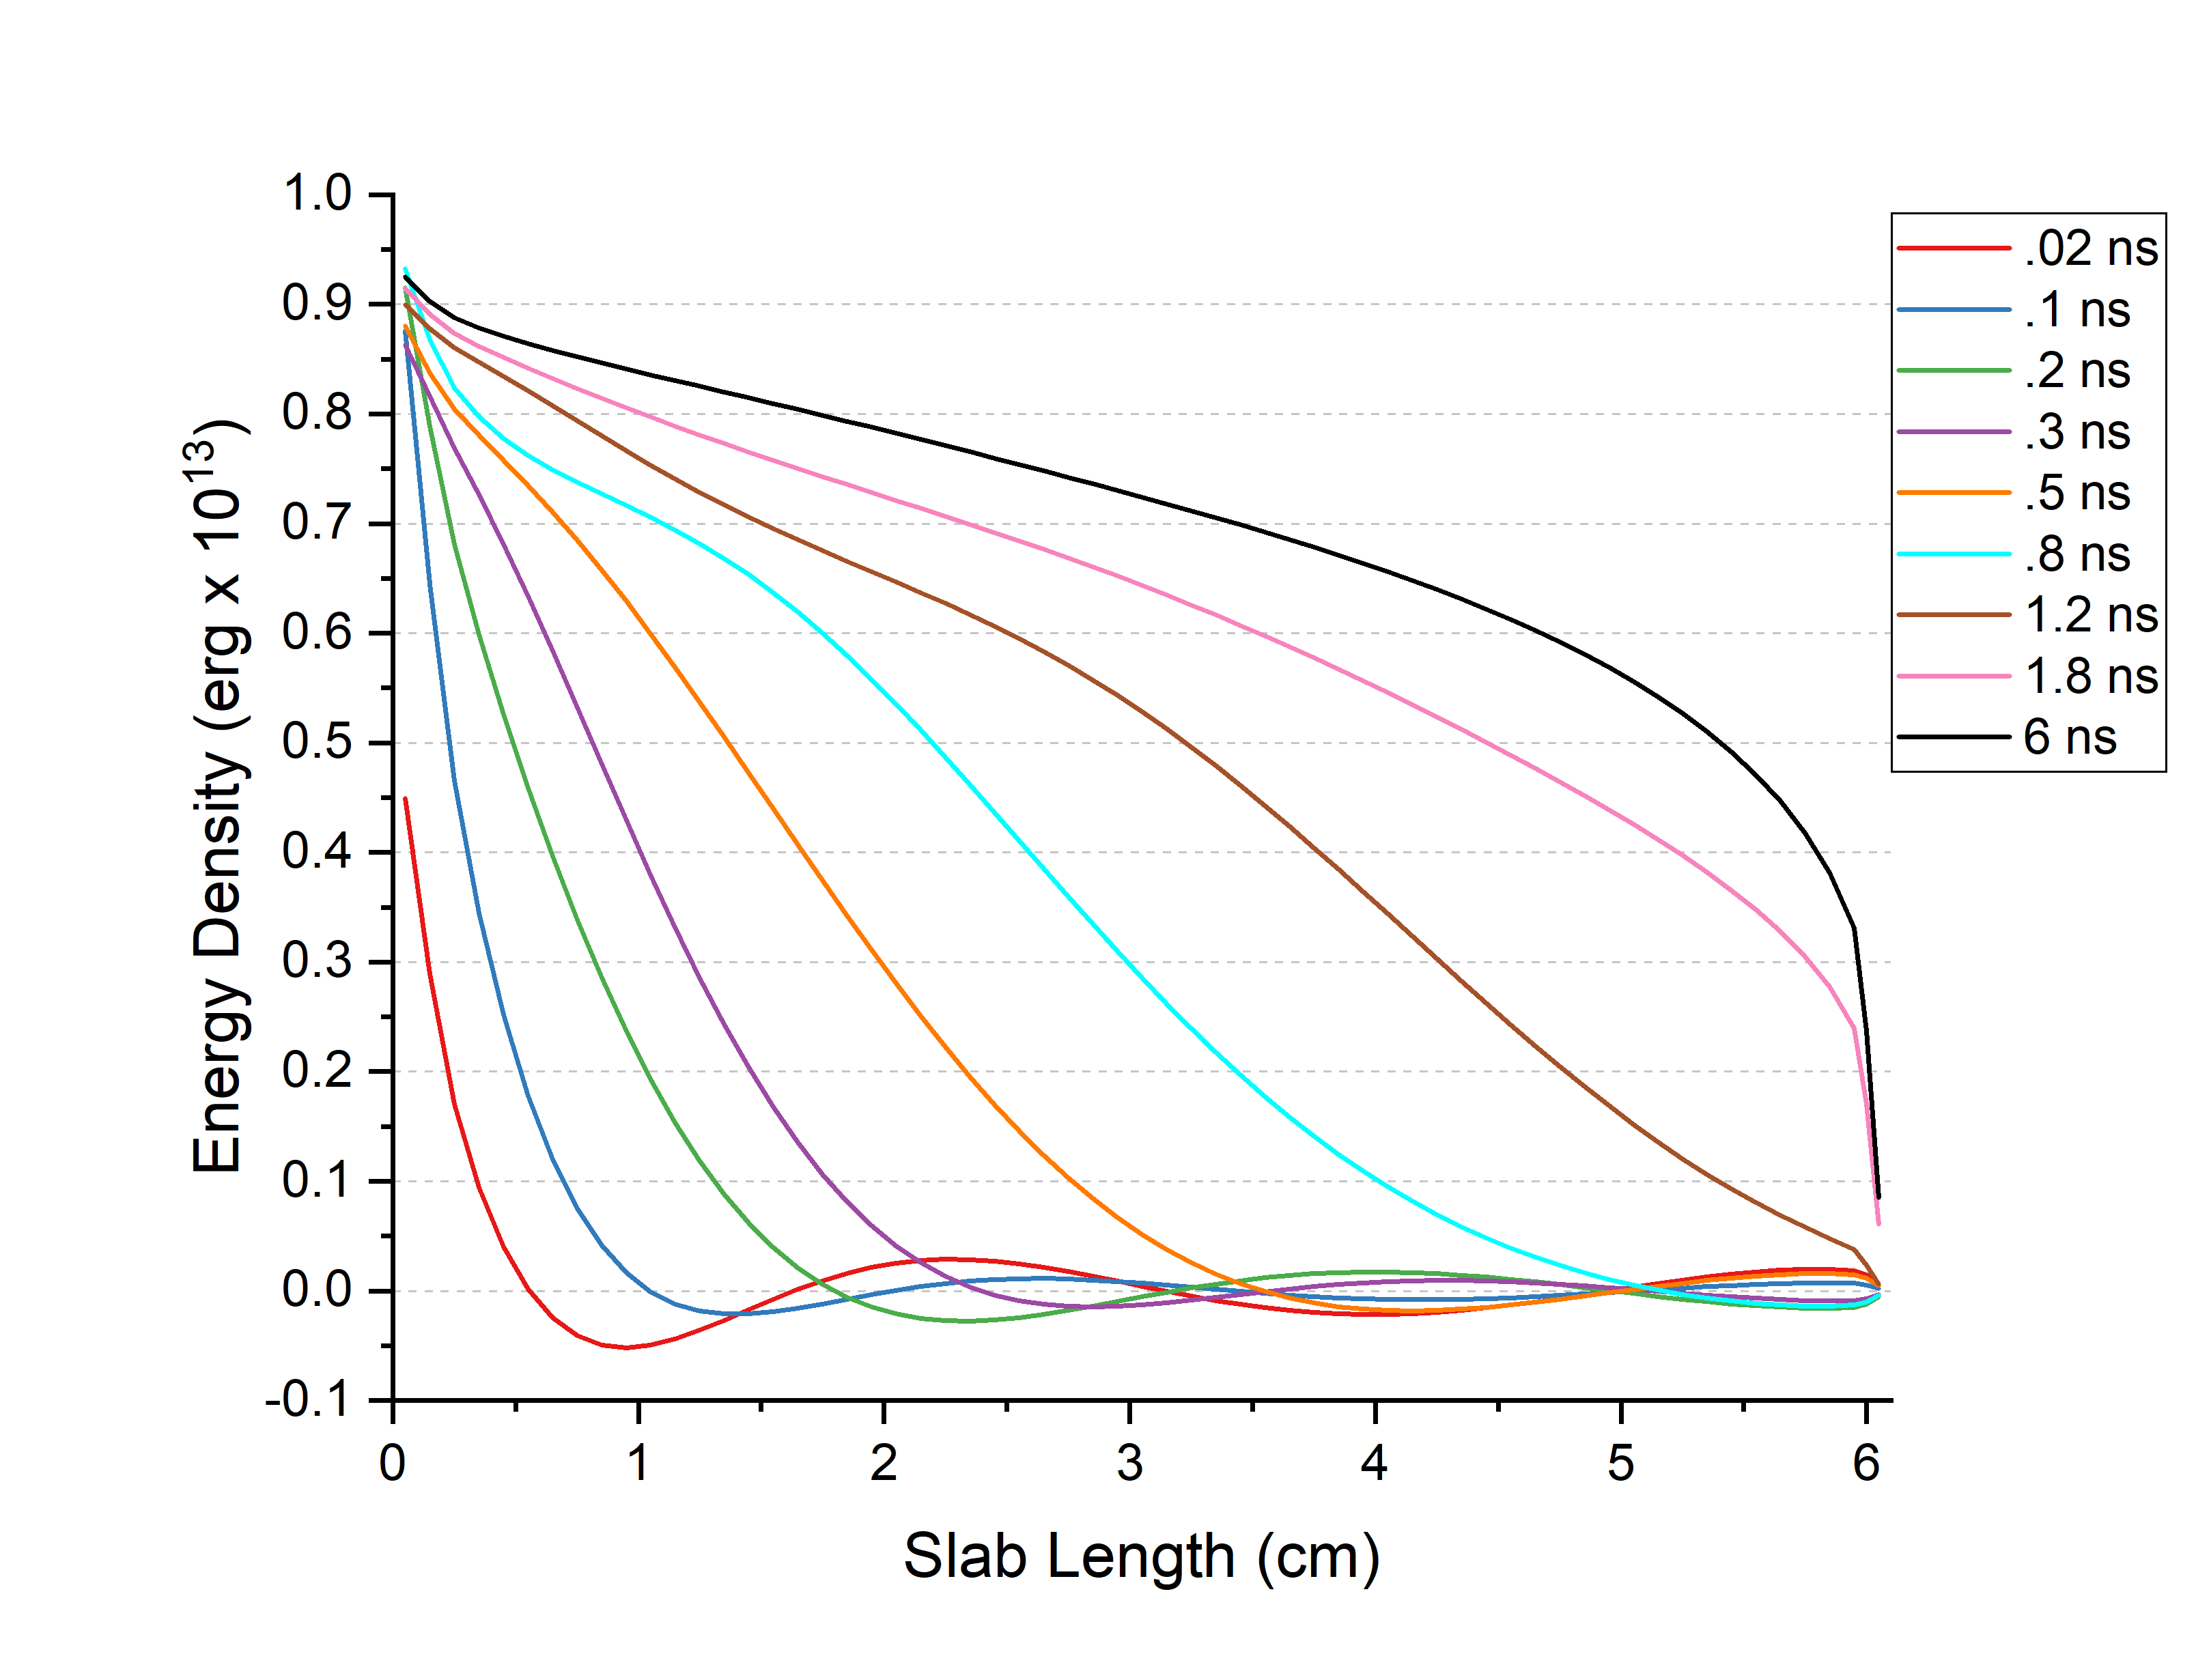
\includegraphics[width=0.5\textwidth]{Eg_g2_cut5_grey.png}}
		\subfloat[r = 10 \label{subfig:Eg_g2_cut10_grey}]{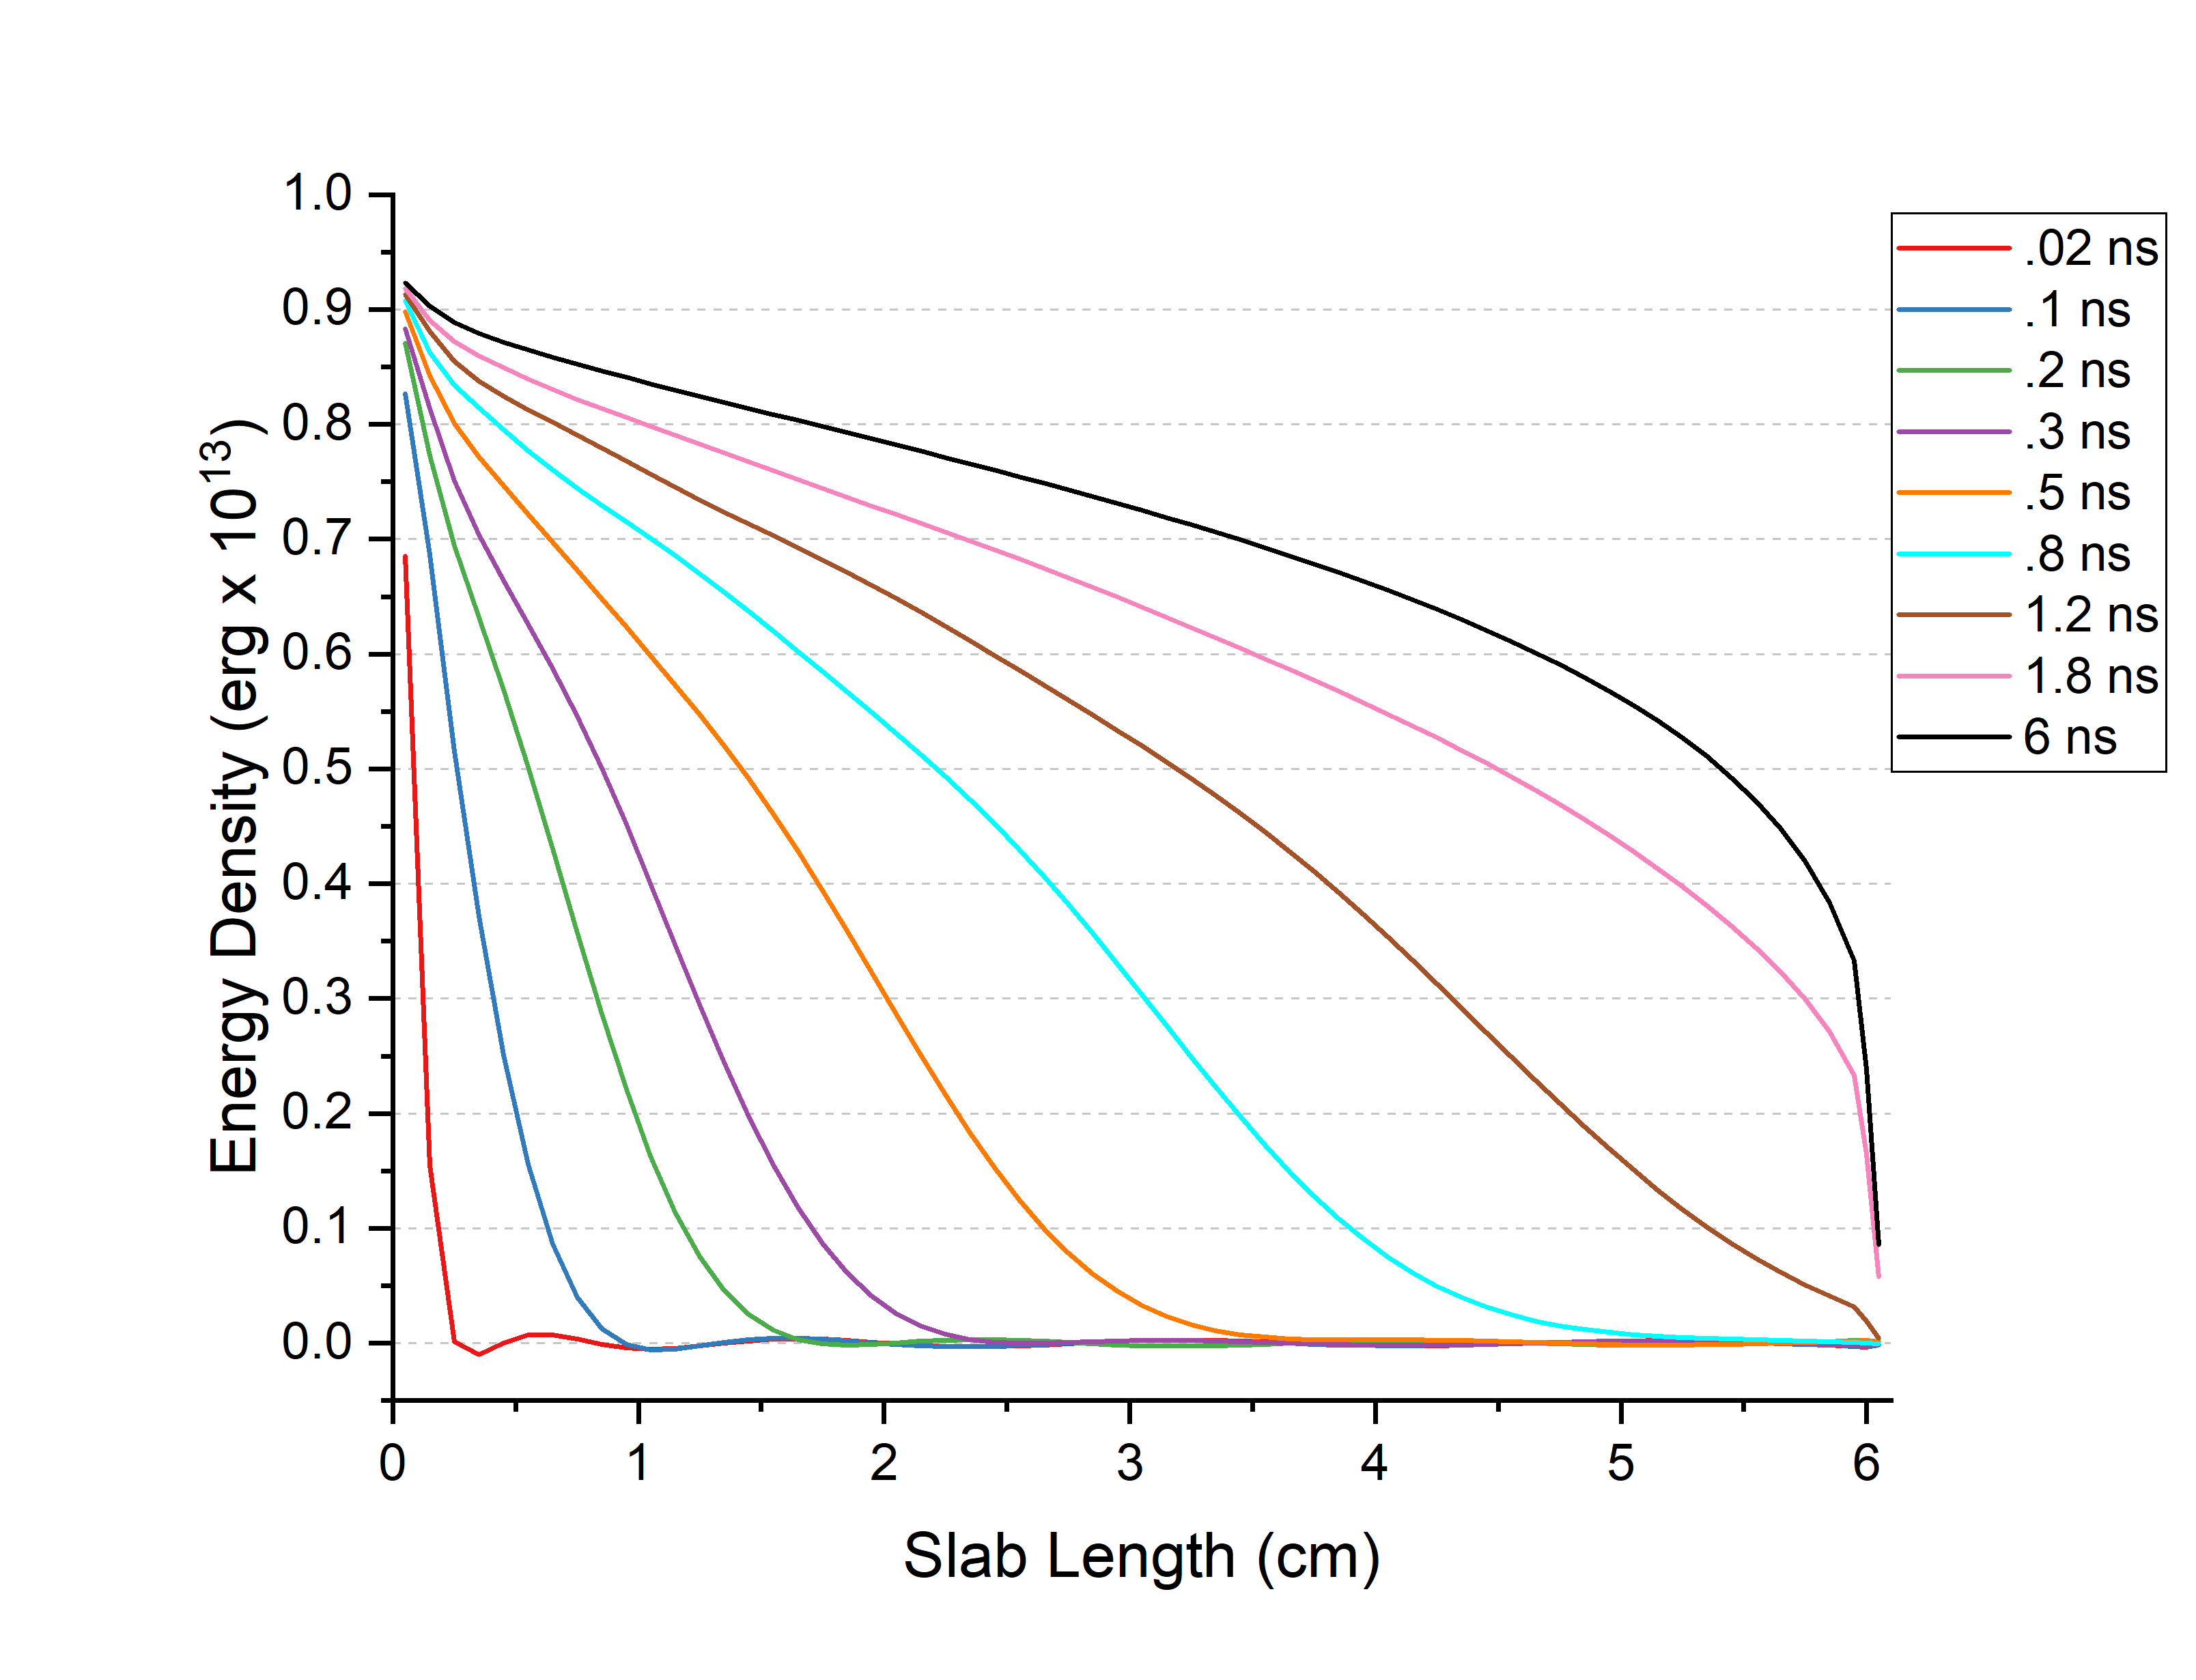
\includegraphics[width=0.5\textwidth]{Eg_g2_cut10_grey.png}}\\
		\subfloat[r = 15 \label{subfig:Eg_g2_cut15_grey}]{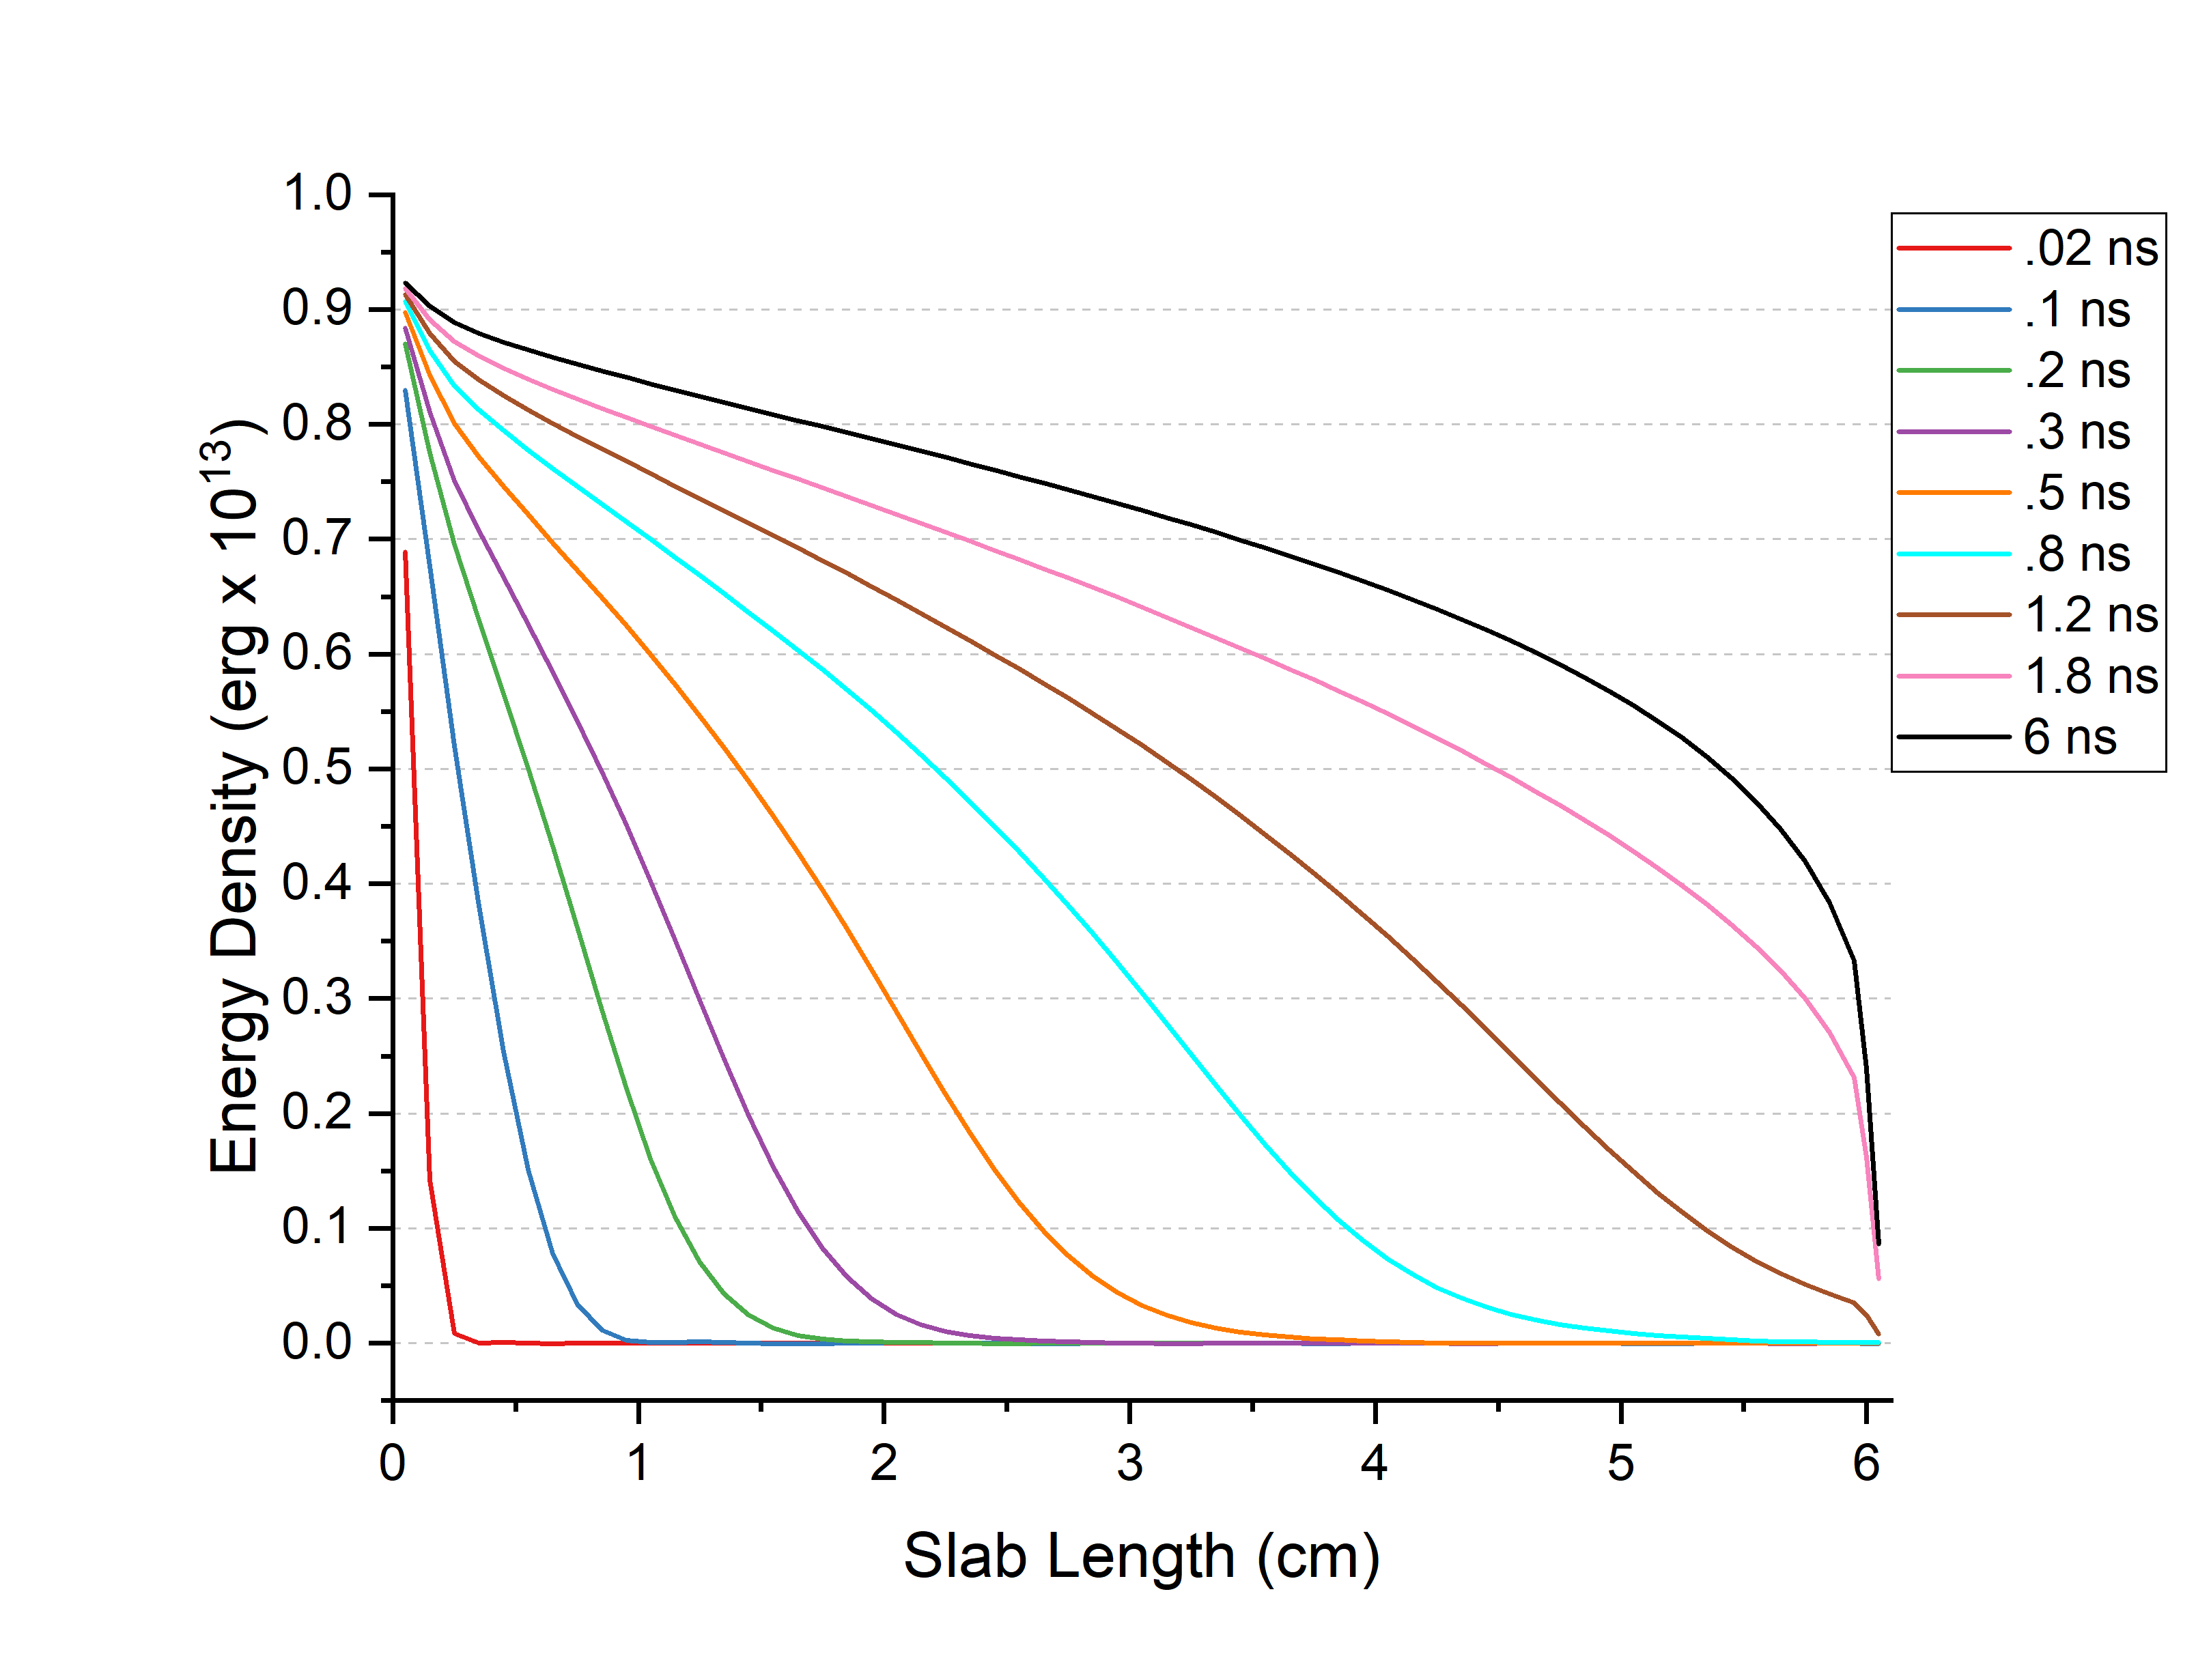
\includegraphics[width=0.5\textwidth]{Eg_g2_cut15_grey.png}}
		\subfloat[r = 20 \label{subfig:Eg_g2_cut20_grey}]{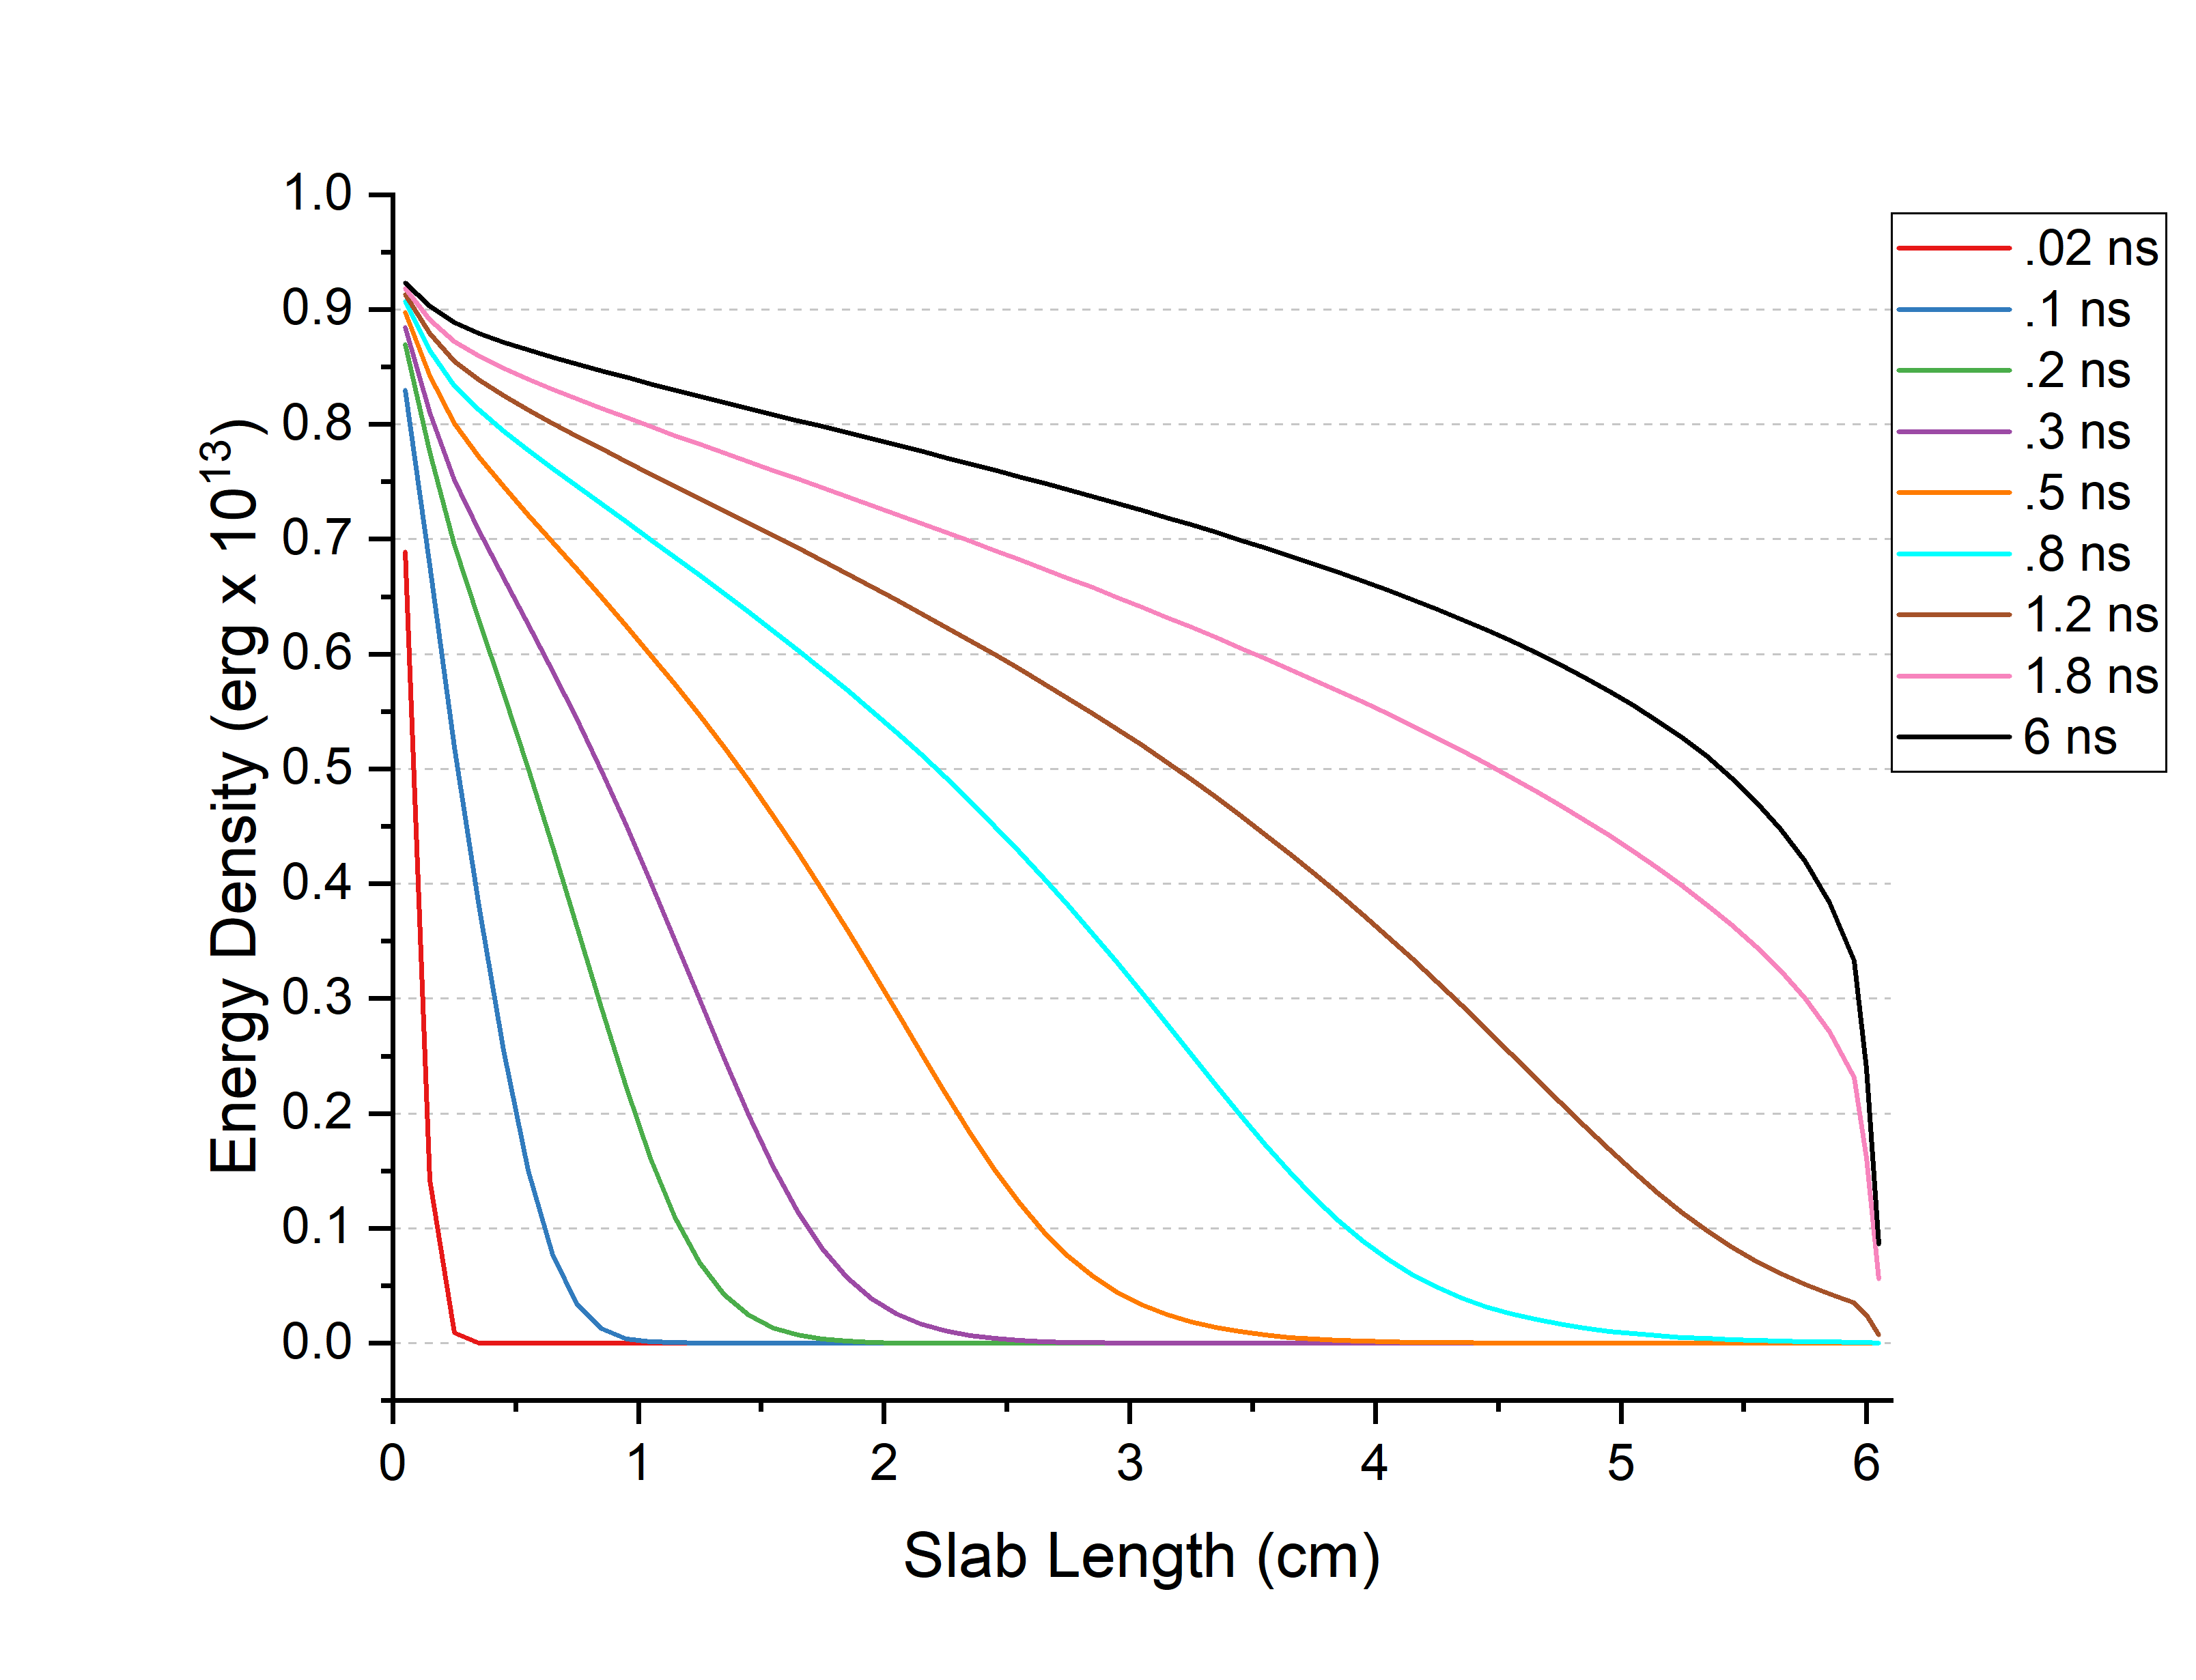
\includegraphics[width=0.5\textwidth]{Eg_g2_cut20_grey.png}}
		\caption{\label{fig:Eg_g2_recomps}
			Low-rank approximations of the group radiation energy density ($E_g^*$) based on the POD for $g=2$ for select time steps}
	\end{figure}
	
	%=================================================================================
	% Eg G3 RECOMP
	\begin{figure}[ht!]
		\centering
		\subfloat[r = 1 \label{subfig:Eg_g3_cut1_grey}]{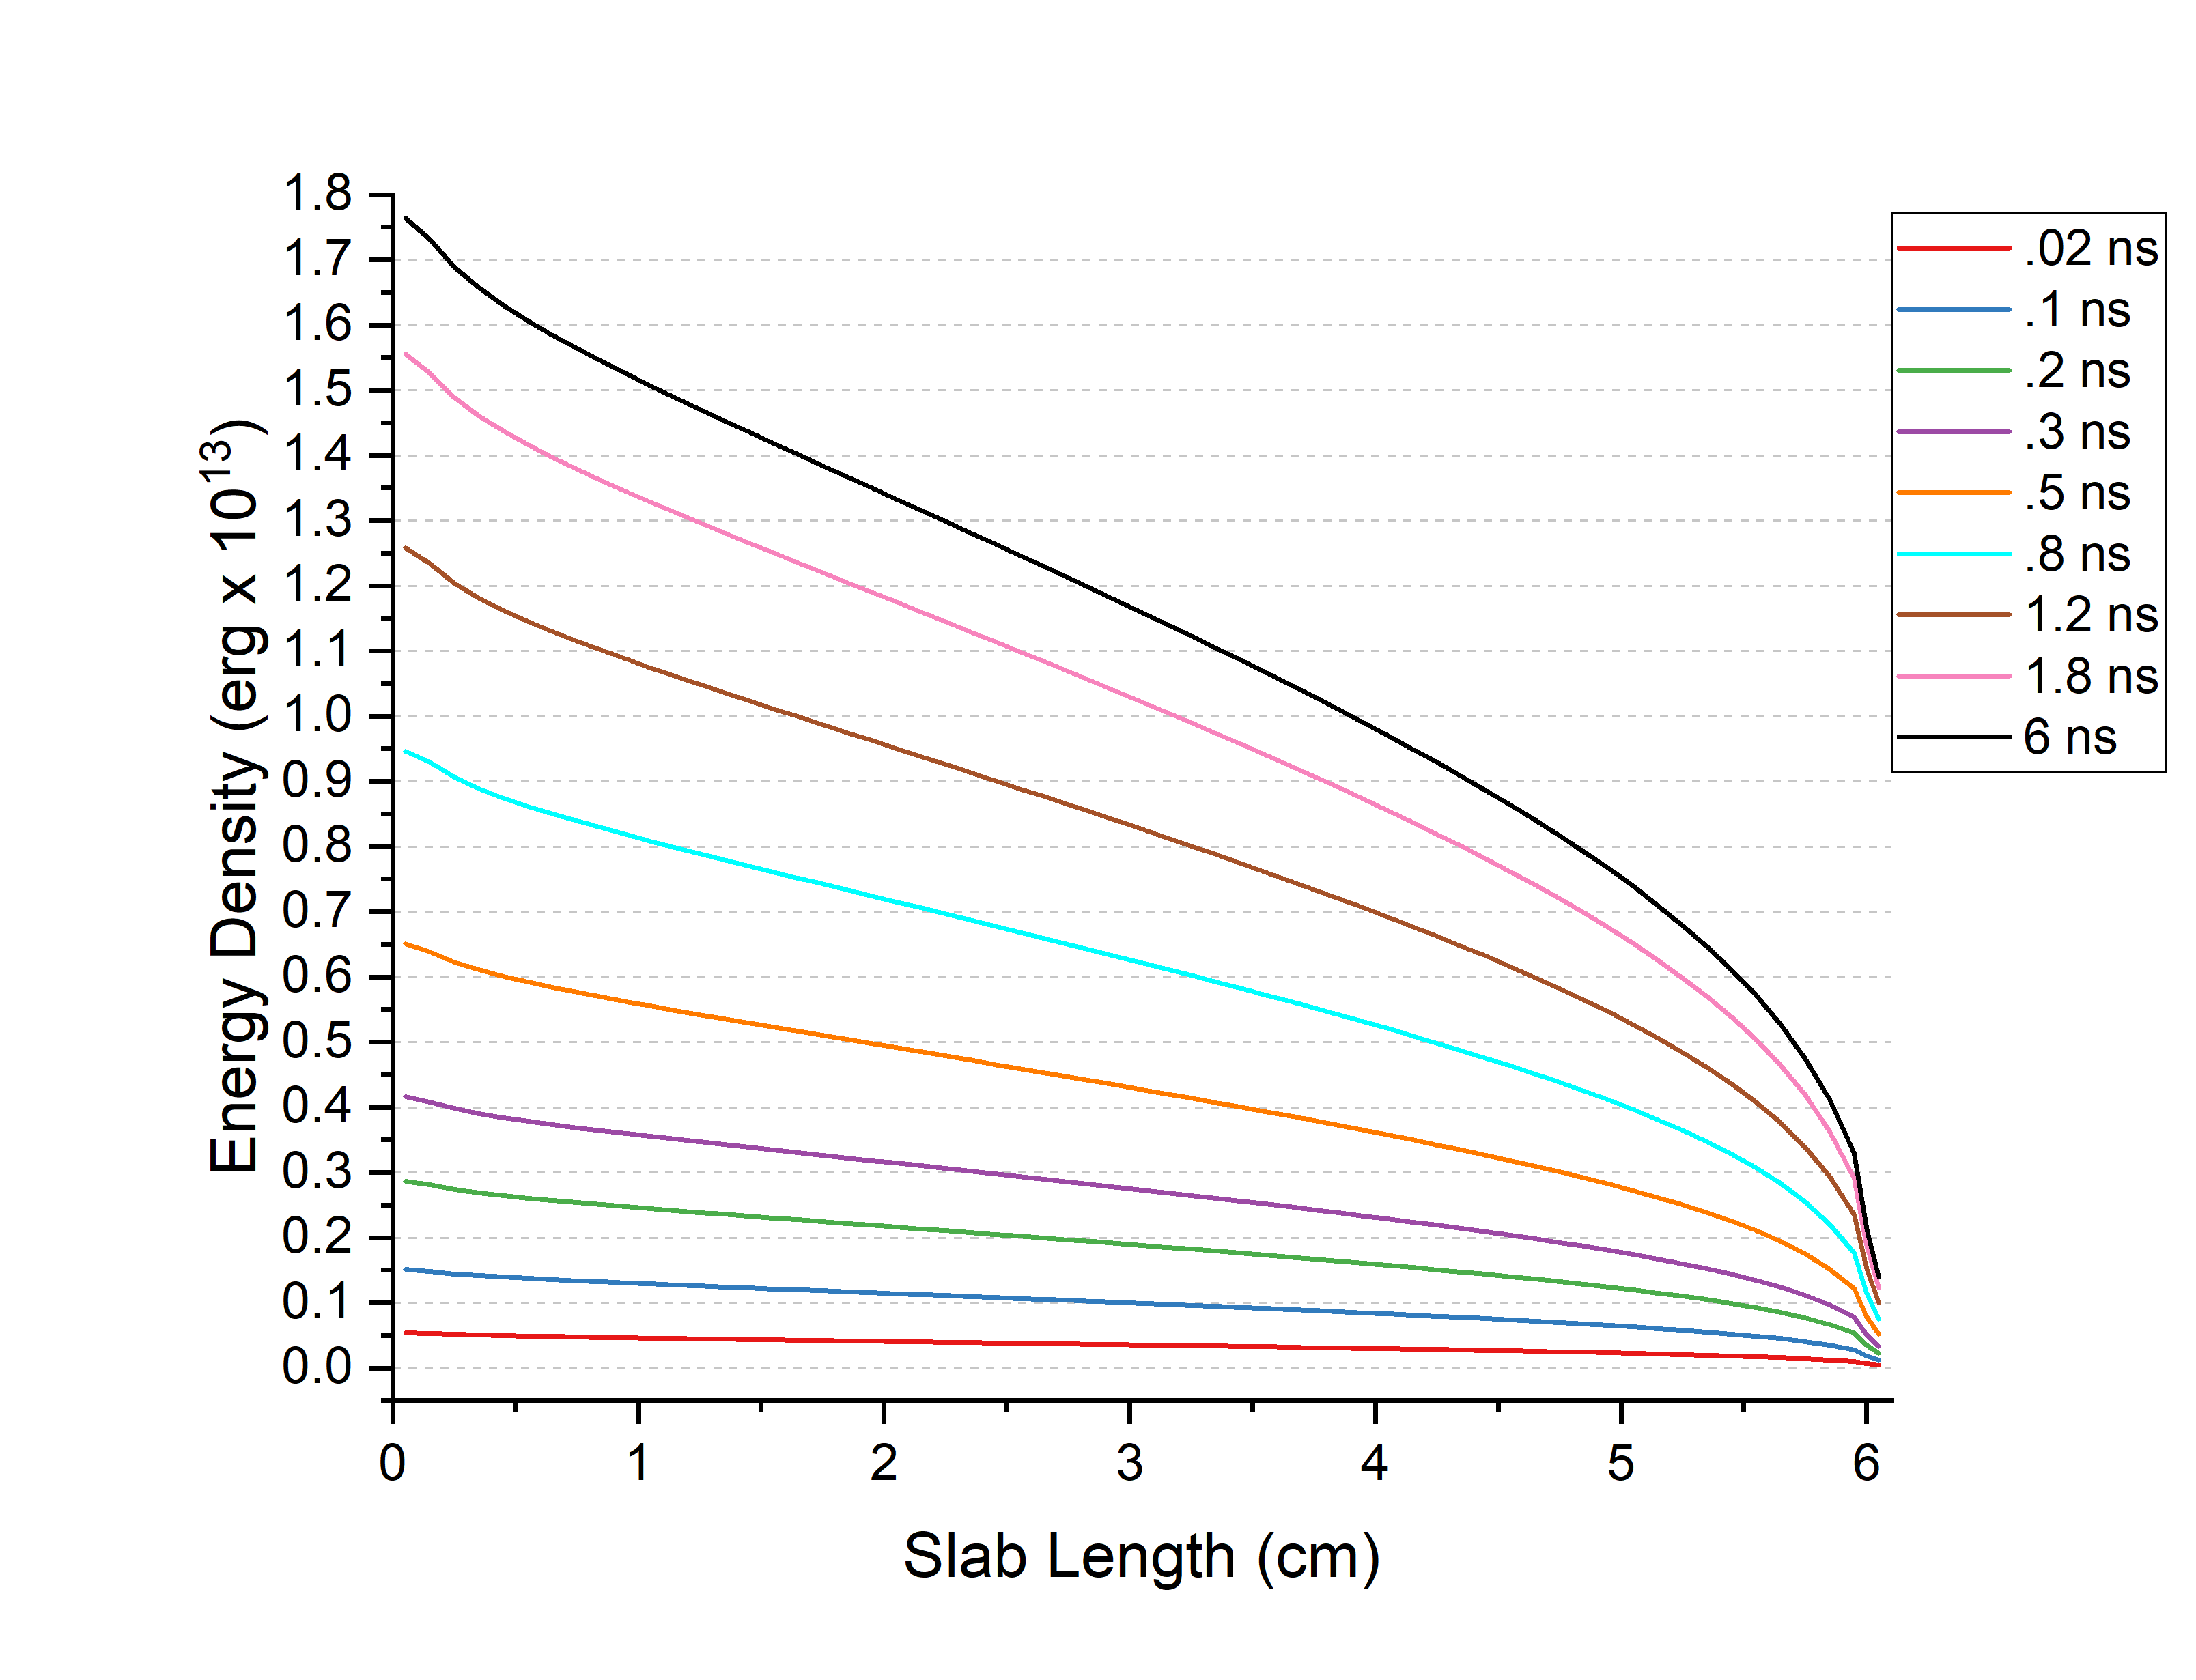
\includegraphics[width=0.5\textwidth]{Eg_g3_cut1_grey.png}}
		\subfloat[r = 2 \label{subfig:Eg_g3_cut2_grey}]{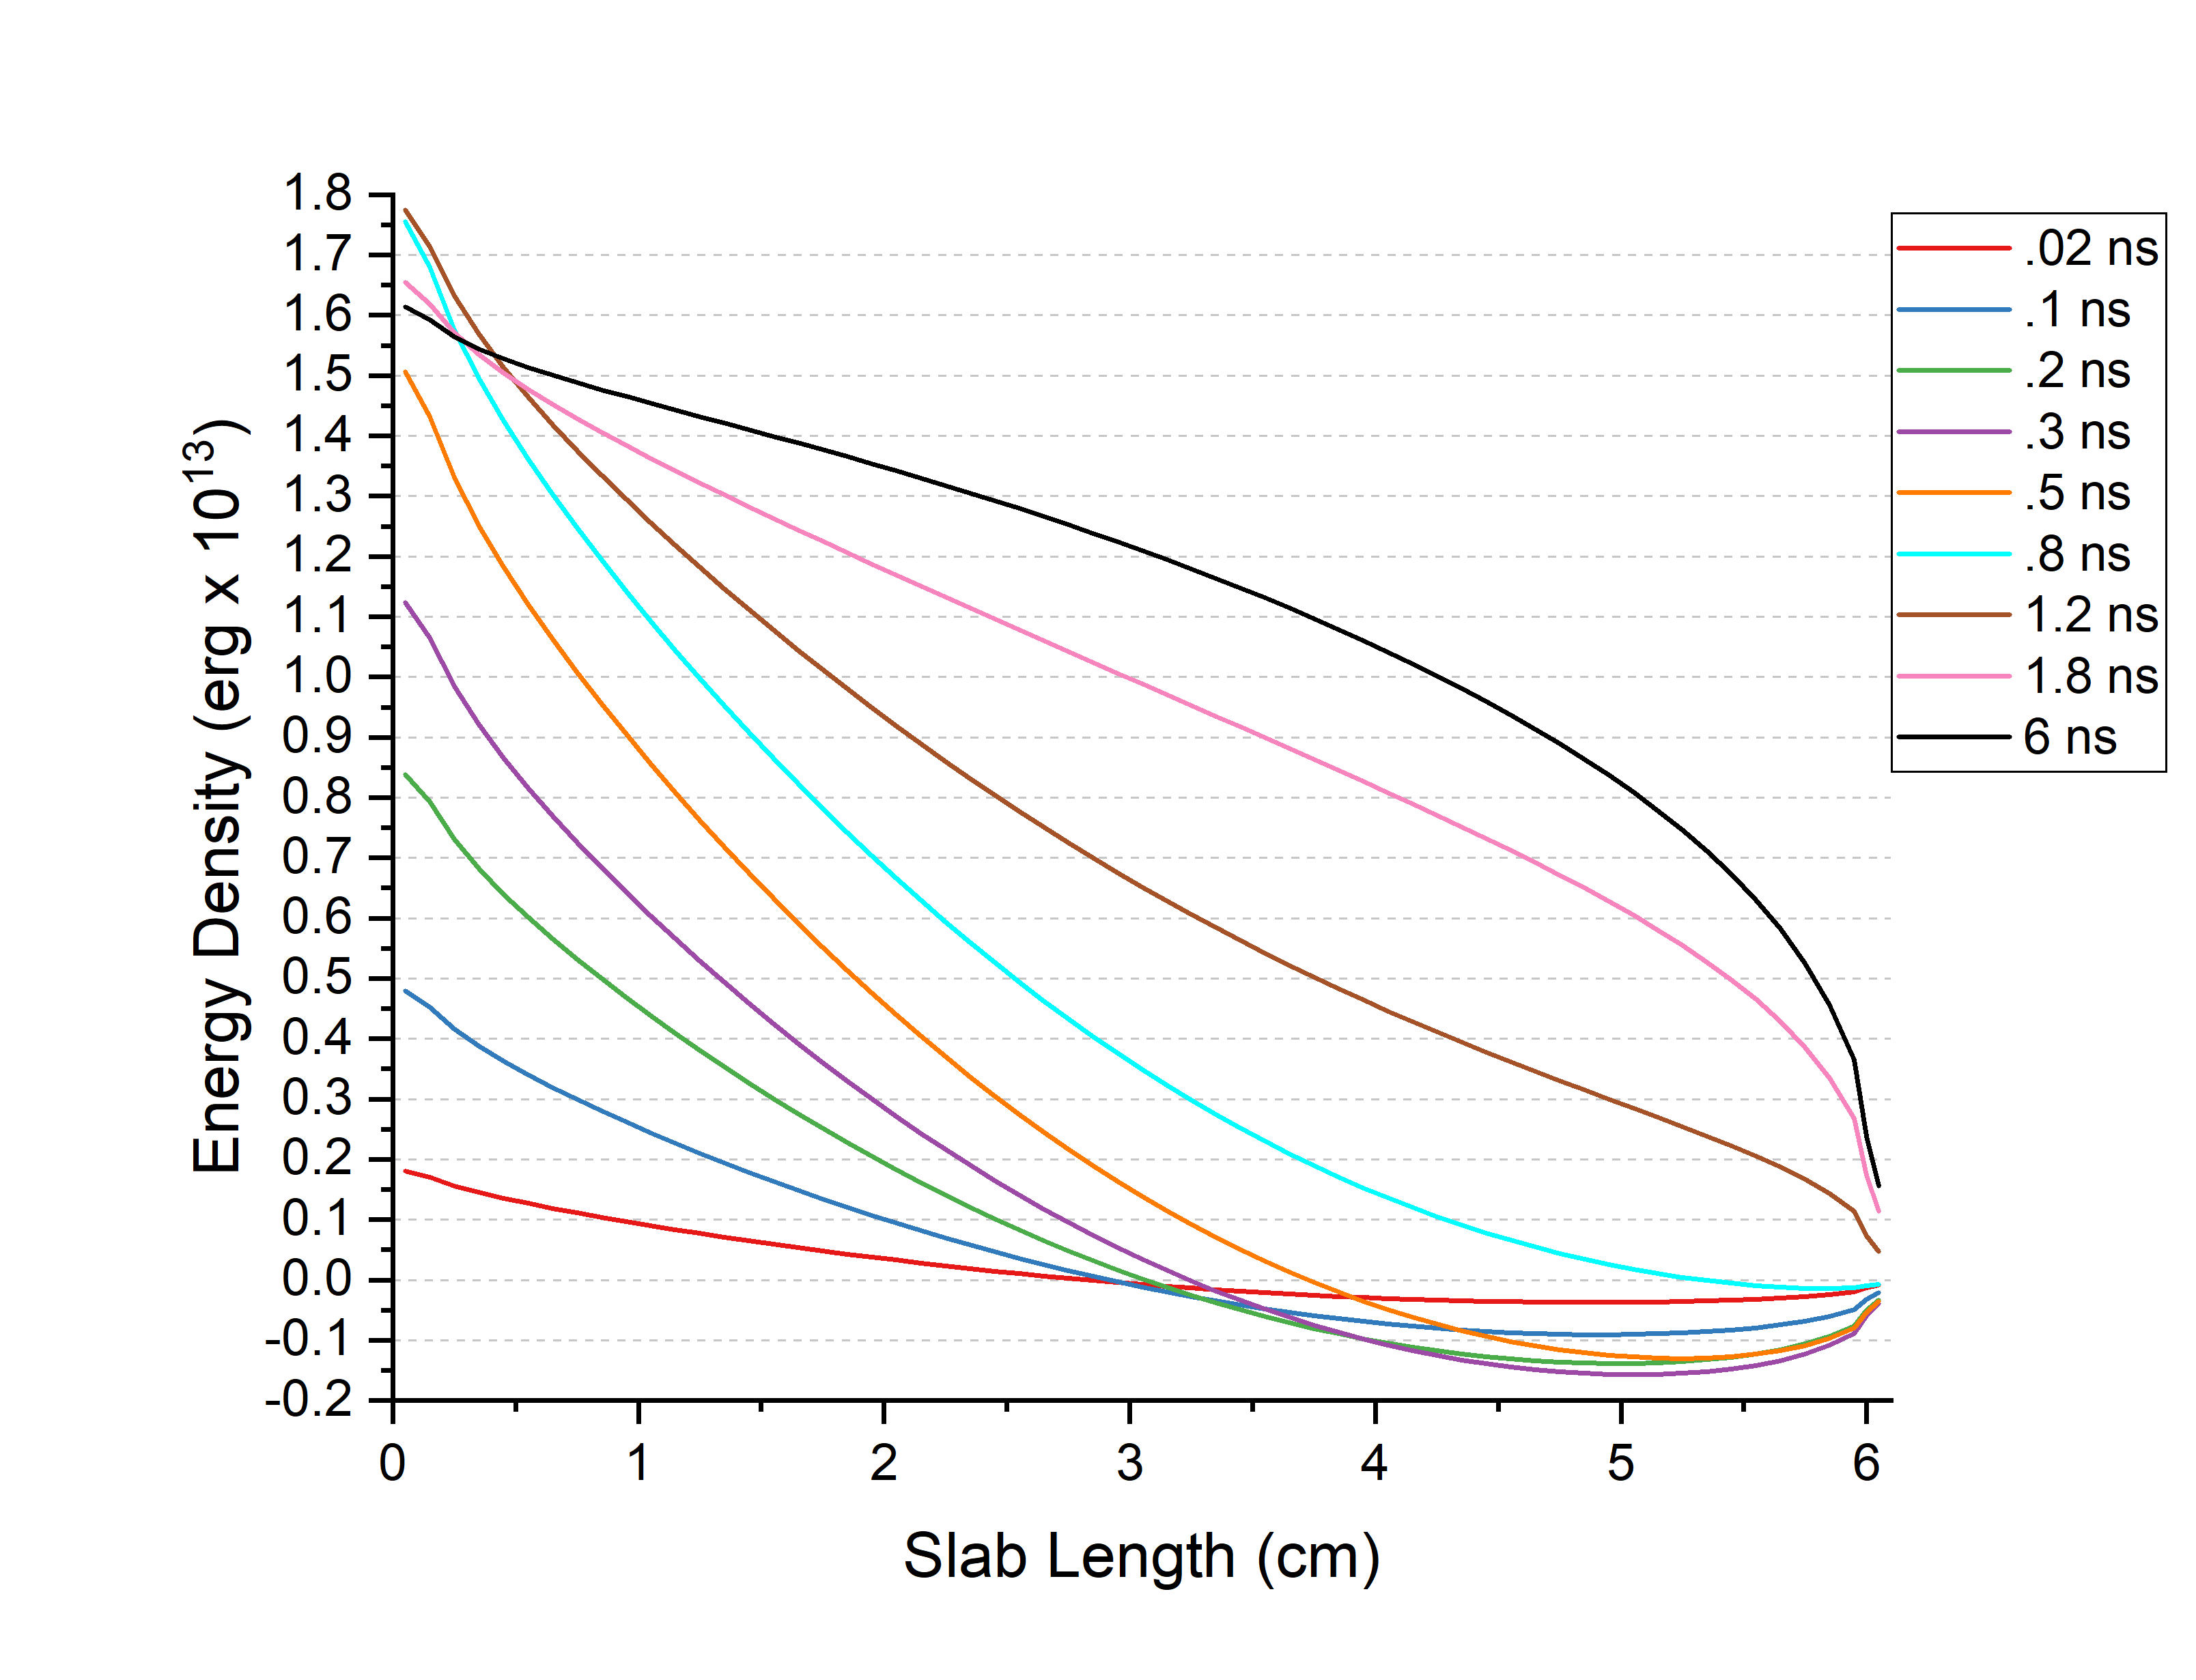
\includegraphics[width=0.5\textwidth]{Eg_g3_cut2_grey.png}}\\
		\subfloat[r = 5 \label{subfig:Eg_g3_cut5_grey}]{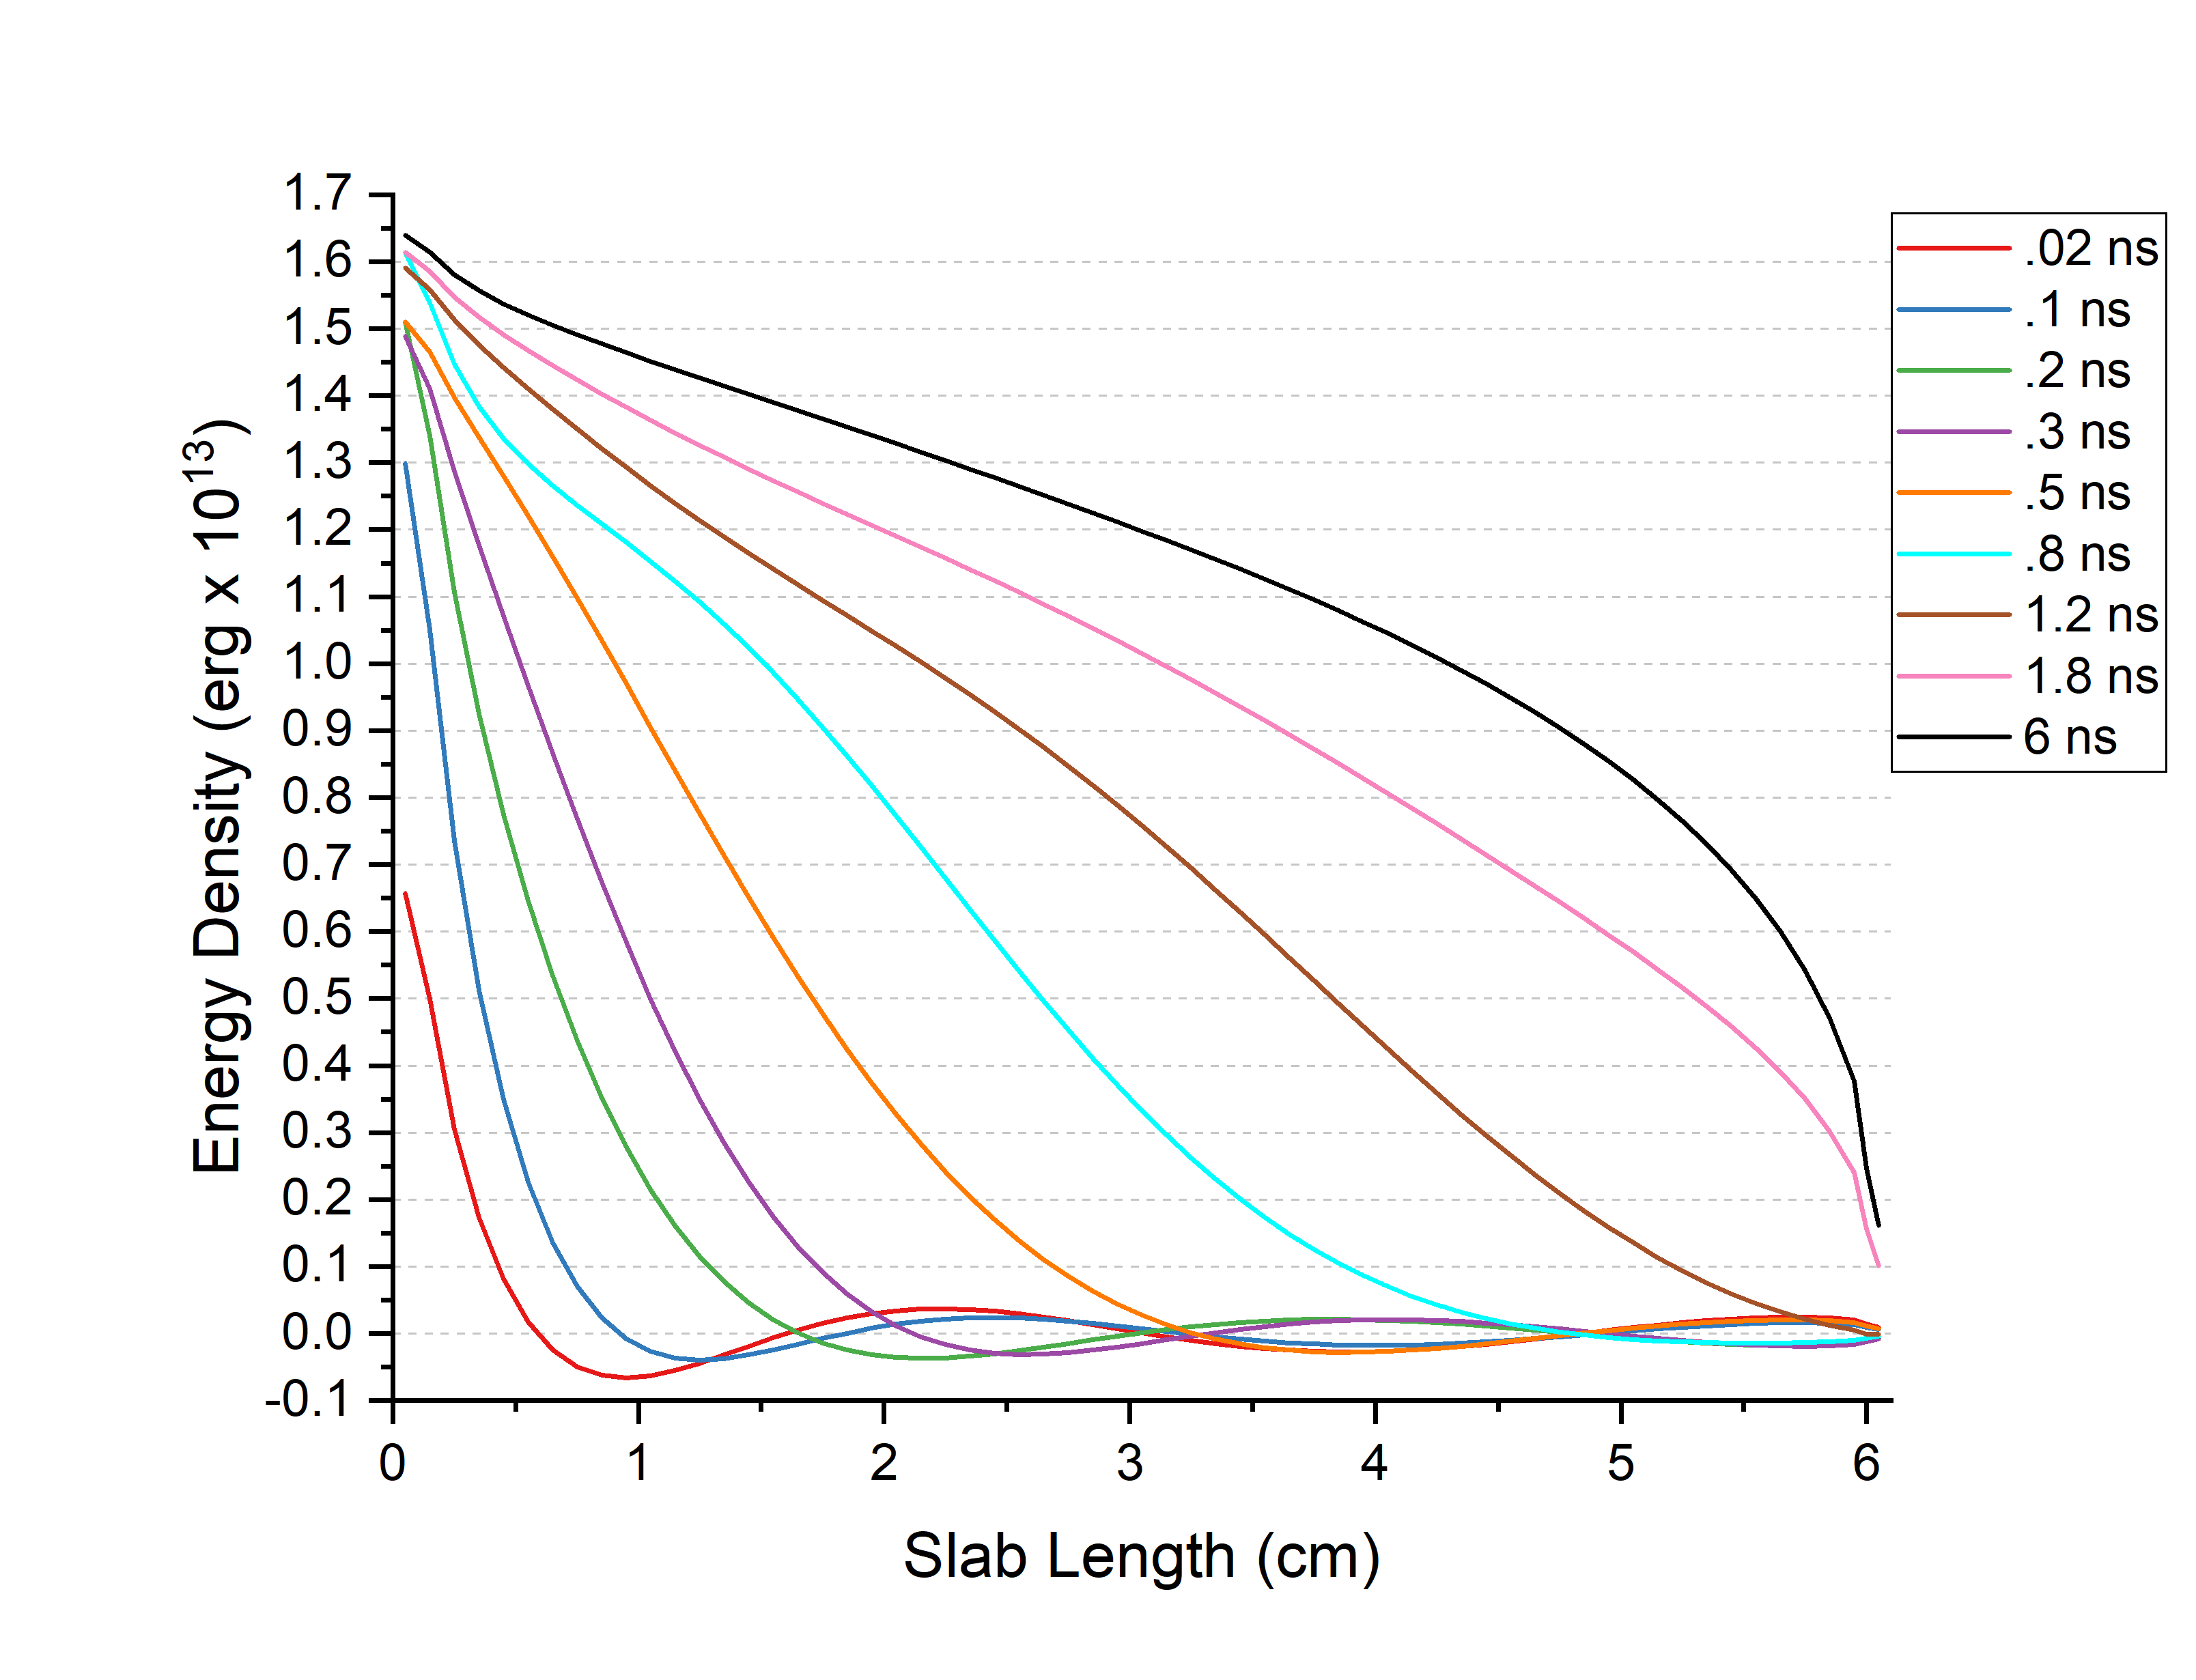
\includegraphics[width=0.5\textwidth]{Eg_g3_cut5_grey.png}}
		\subfloat[r = 10 \label{subfig:Eg_g3_cut10_grey}]{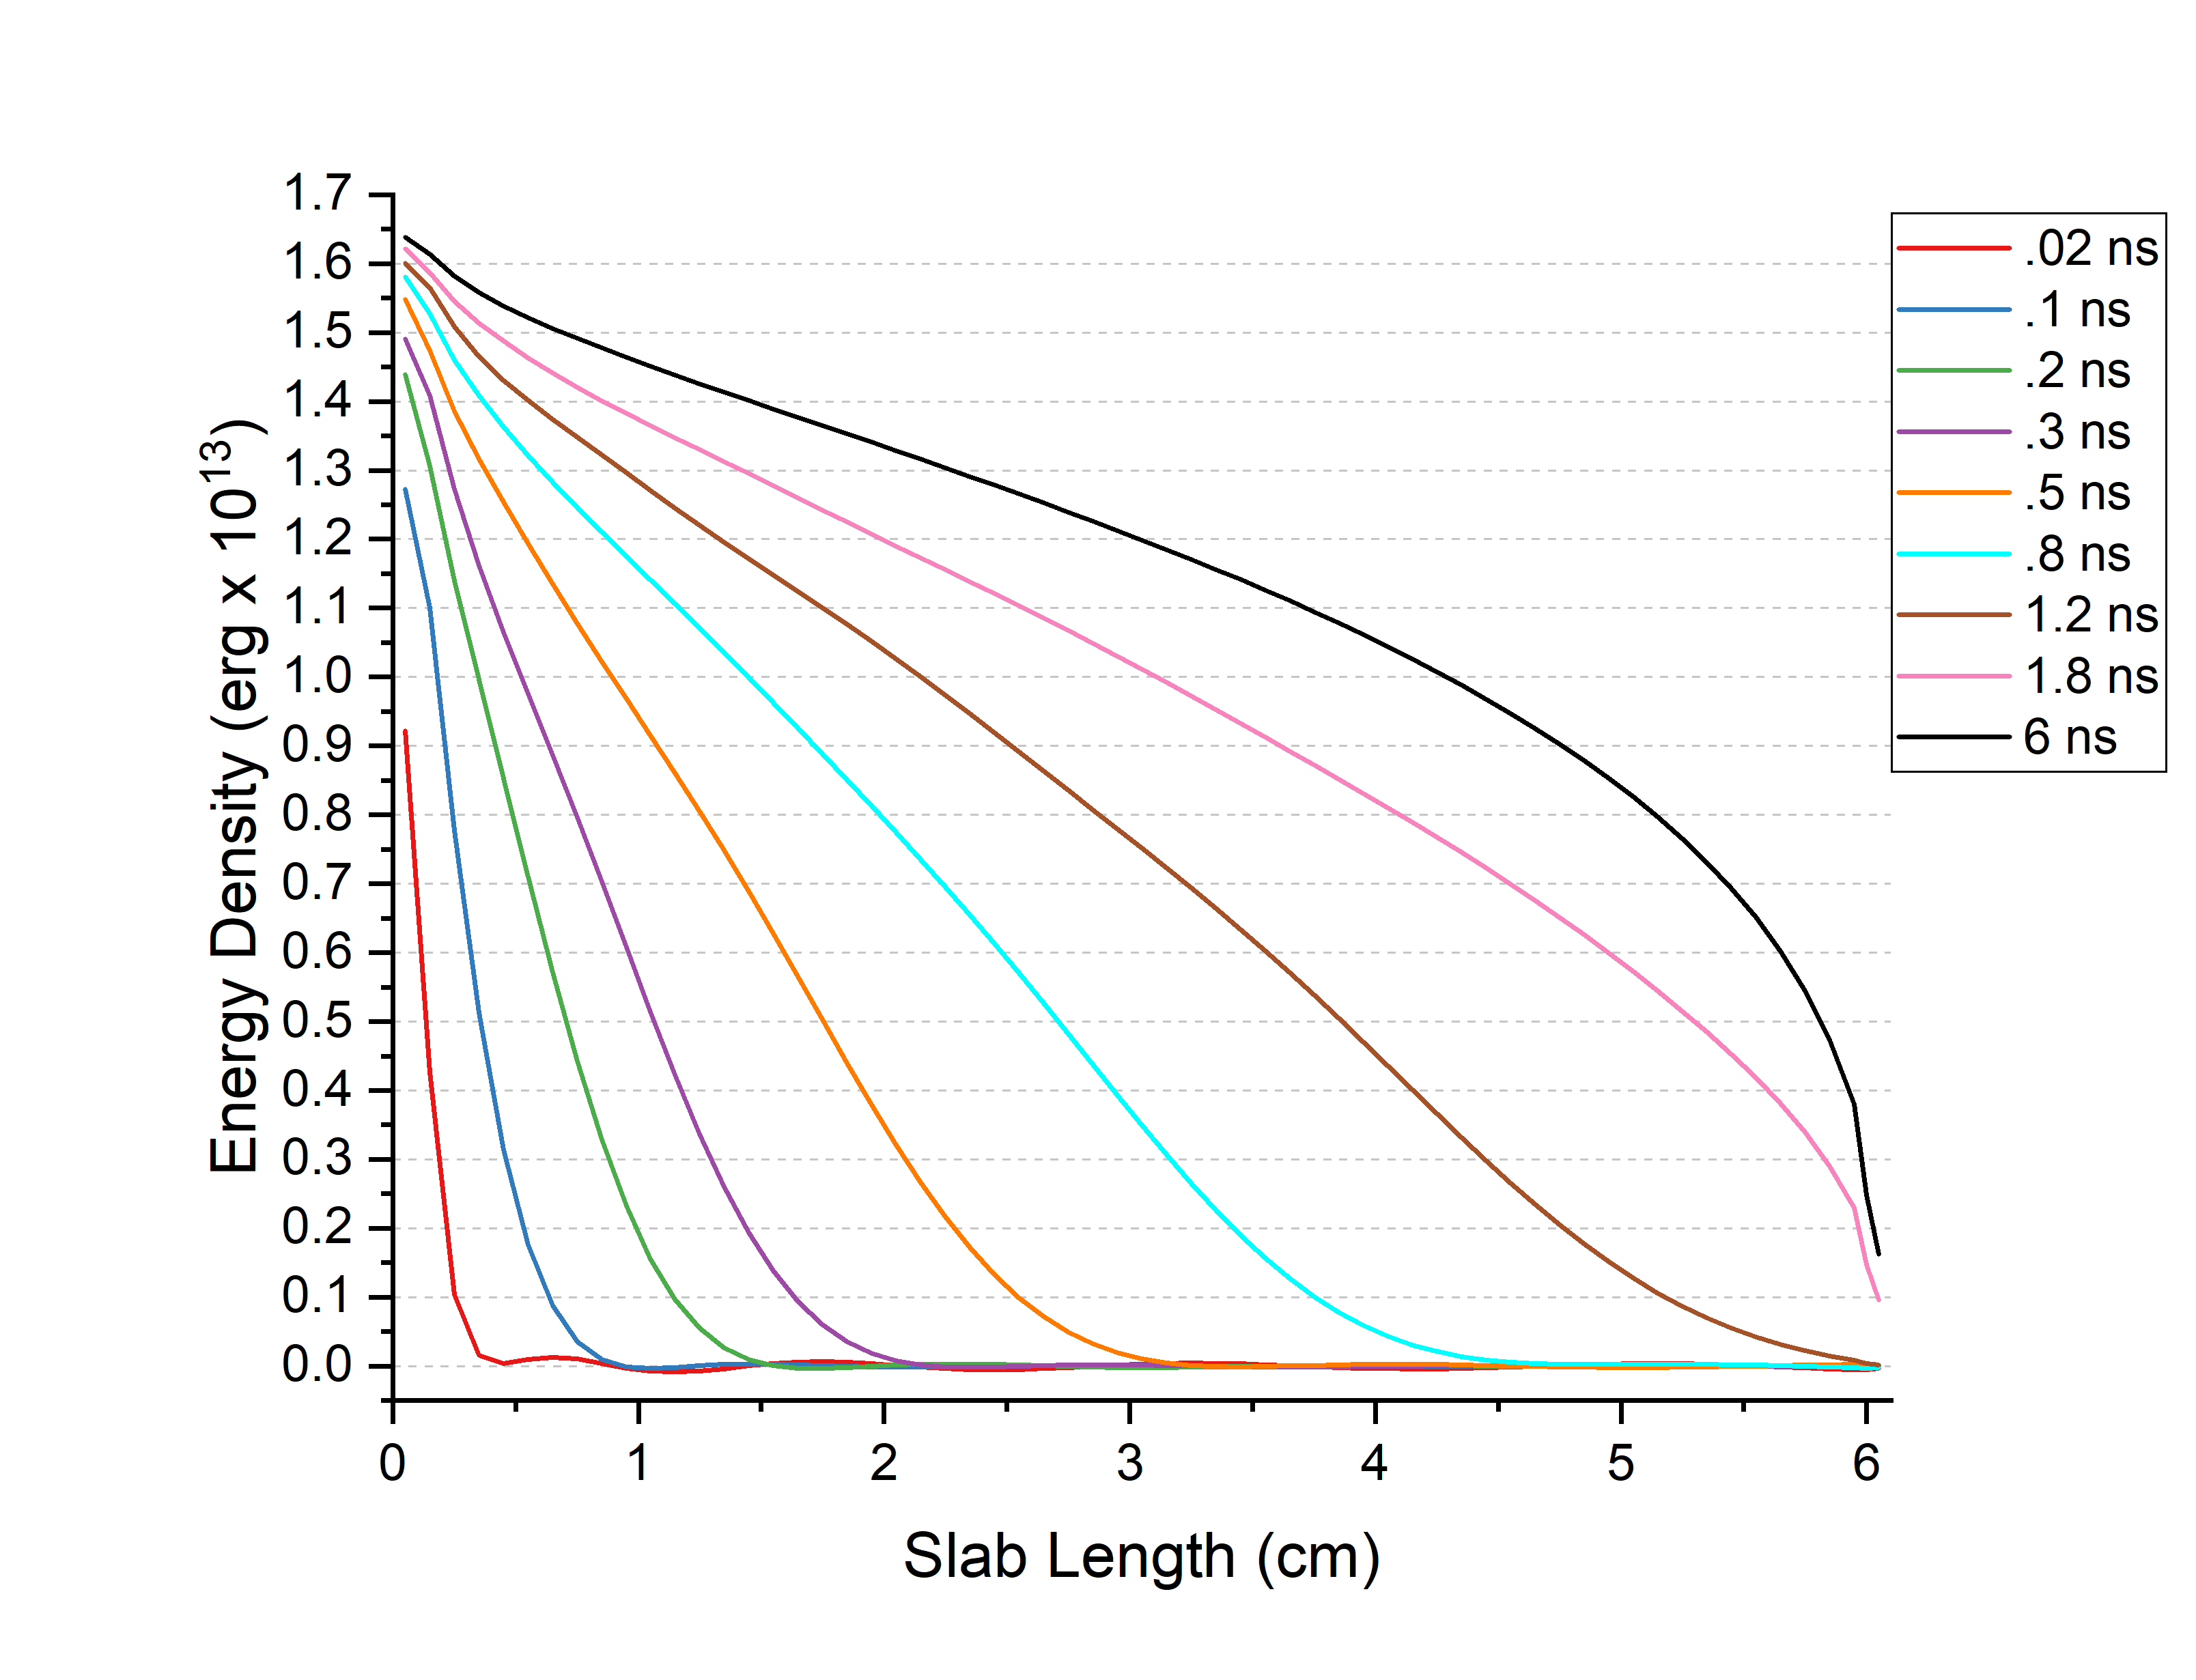
\includegraphics[width=0.5\textwidth]{Eg_g3_cut10_grey.png}}\\
		\subfloat[r = 15 \label{subfig:Eg_g3_cut15_grey}]{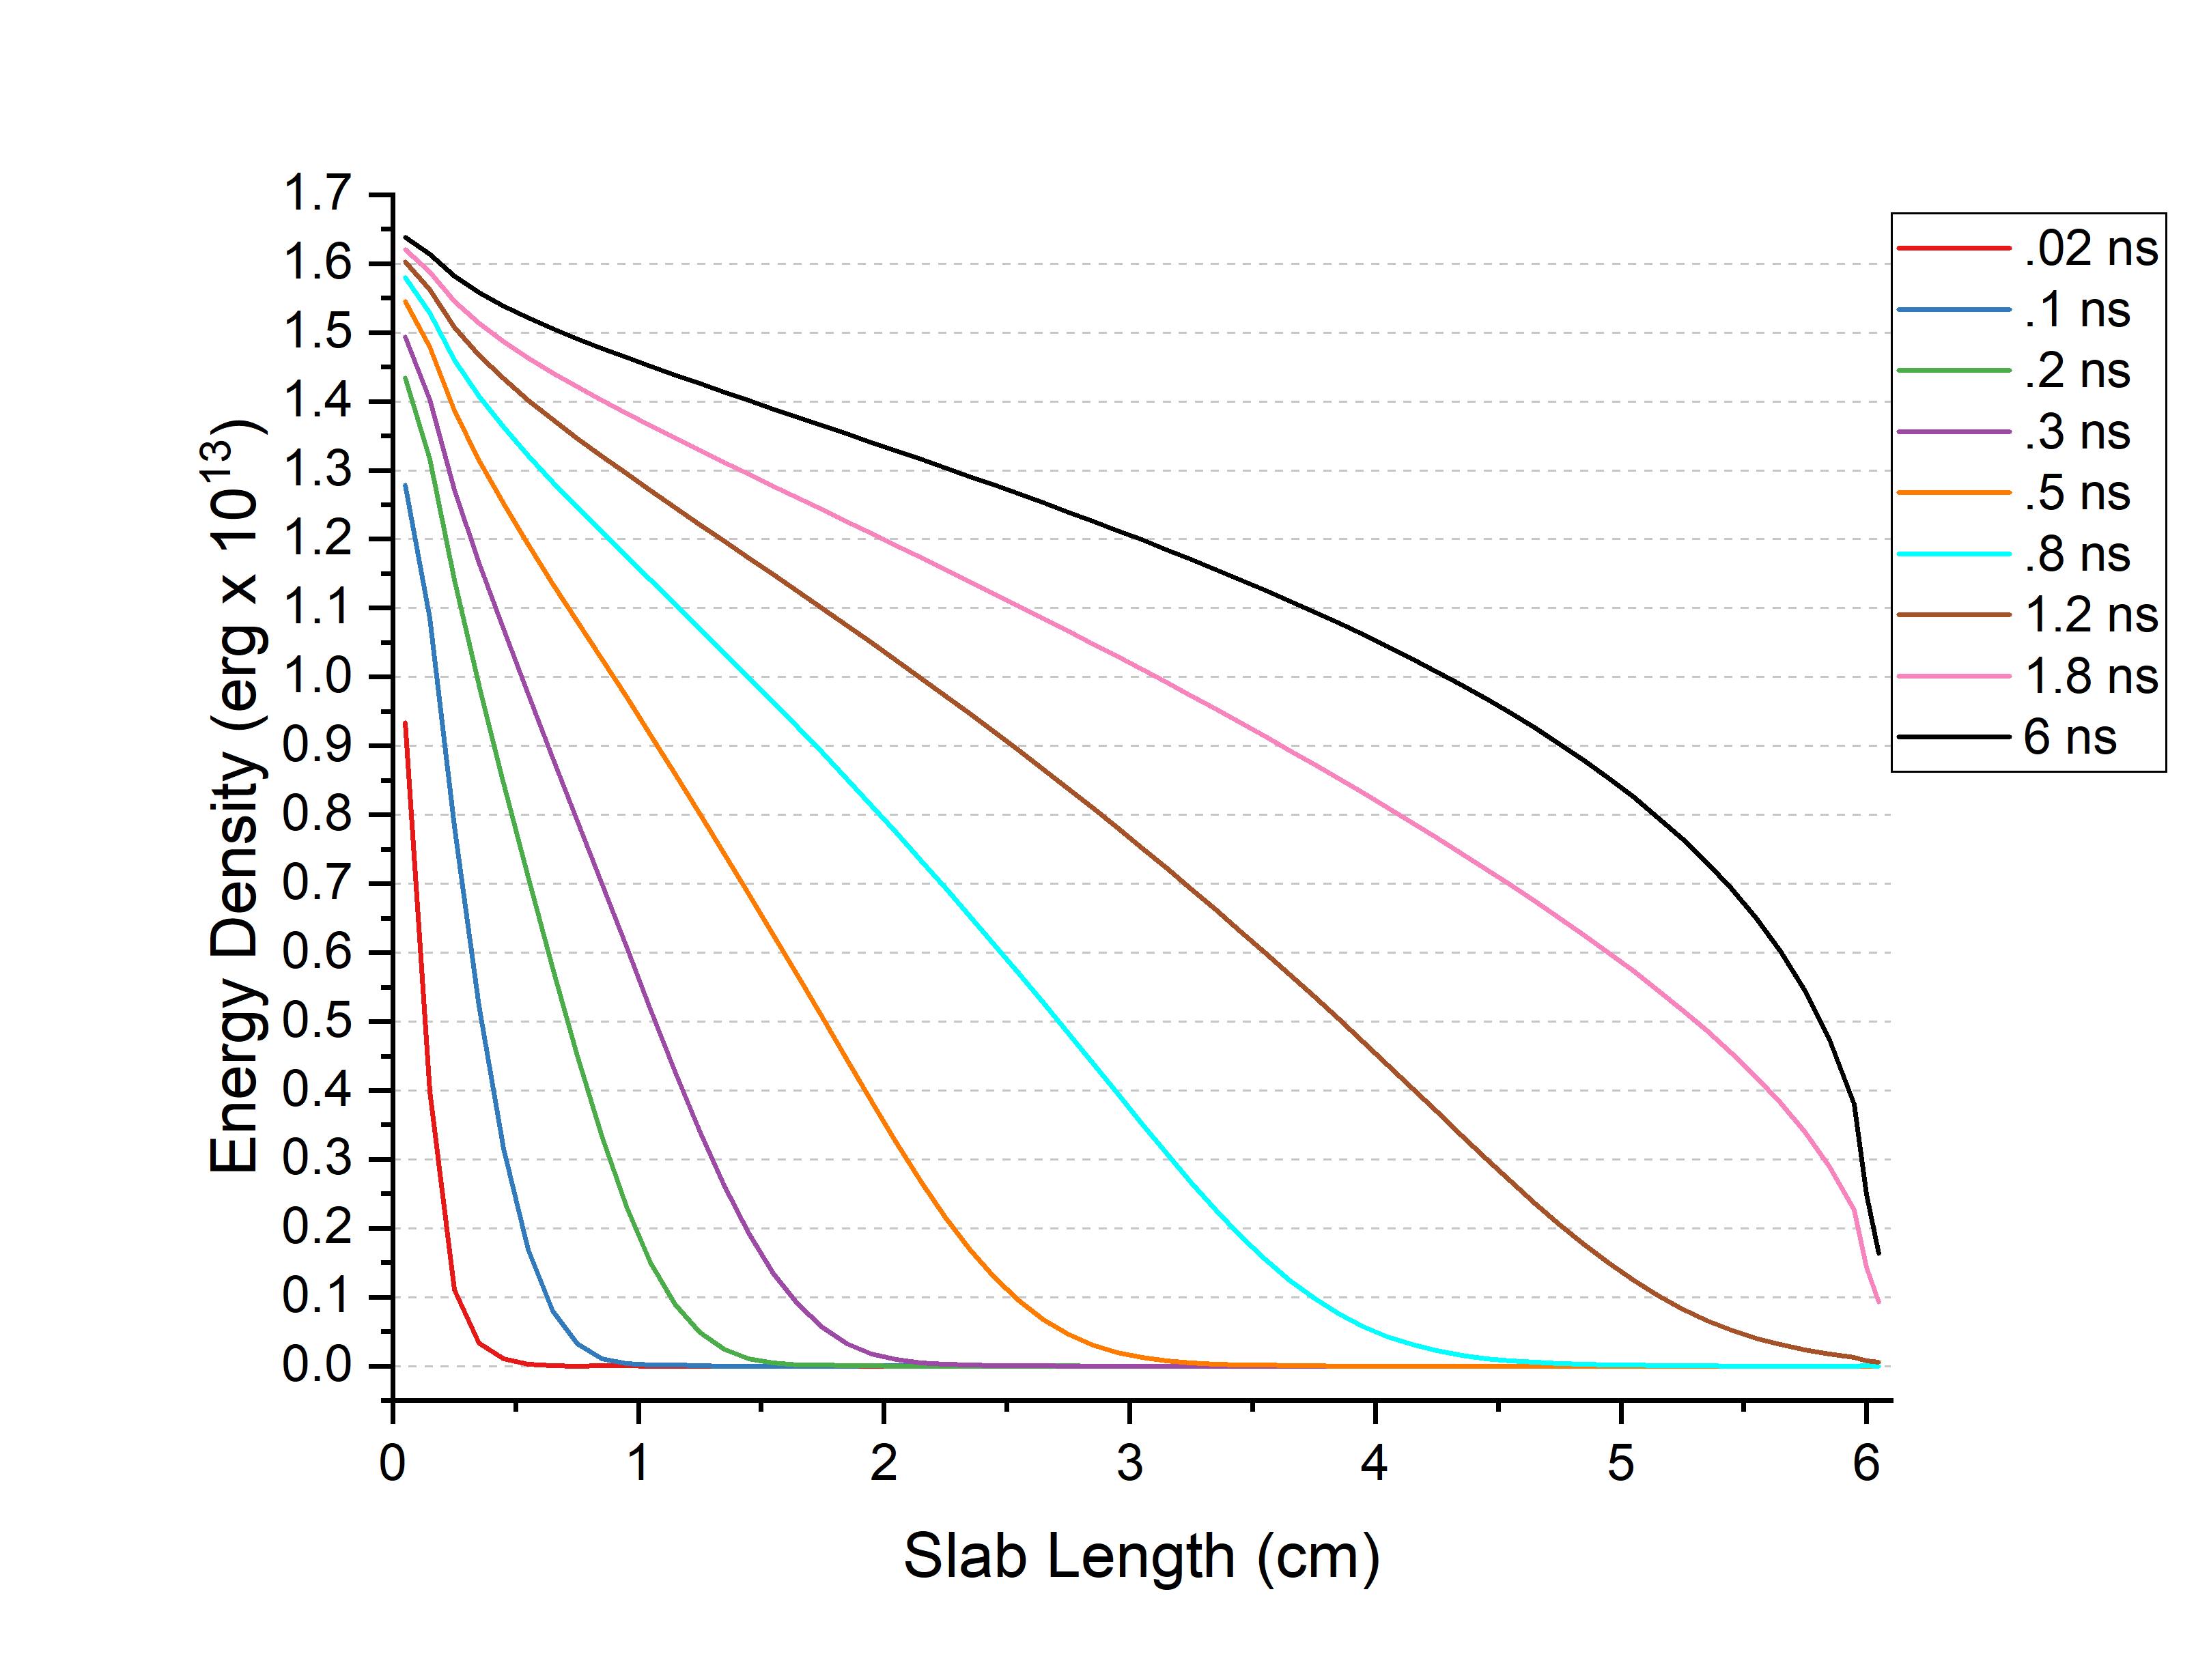
\includegraphics[width=0.5\textwidth]{Eg_g3_cut15_grey.png}}
		\subfloat[r = 20 \label{subfig:Eg_g3_cut20_grey}]{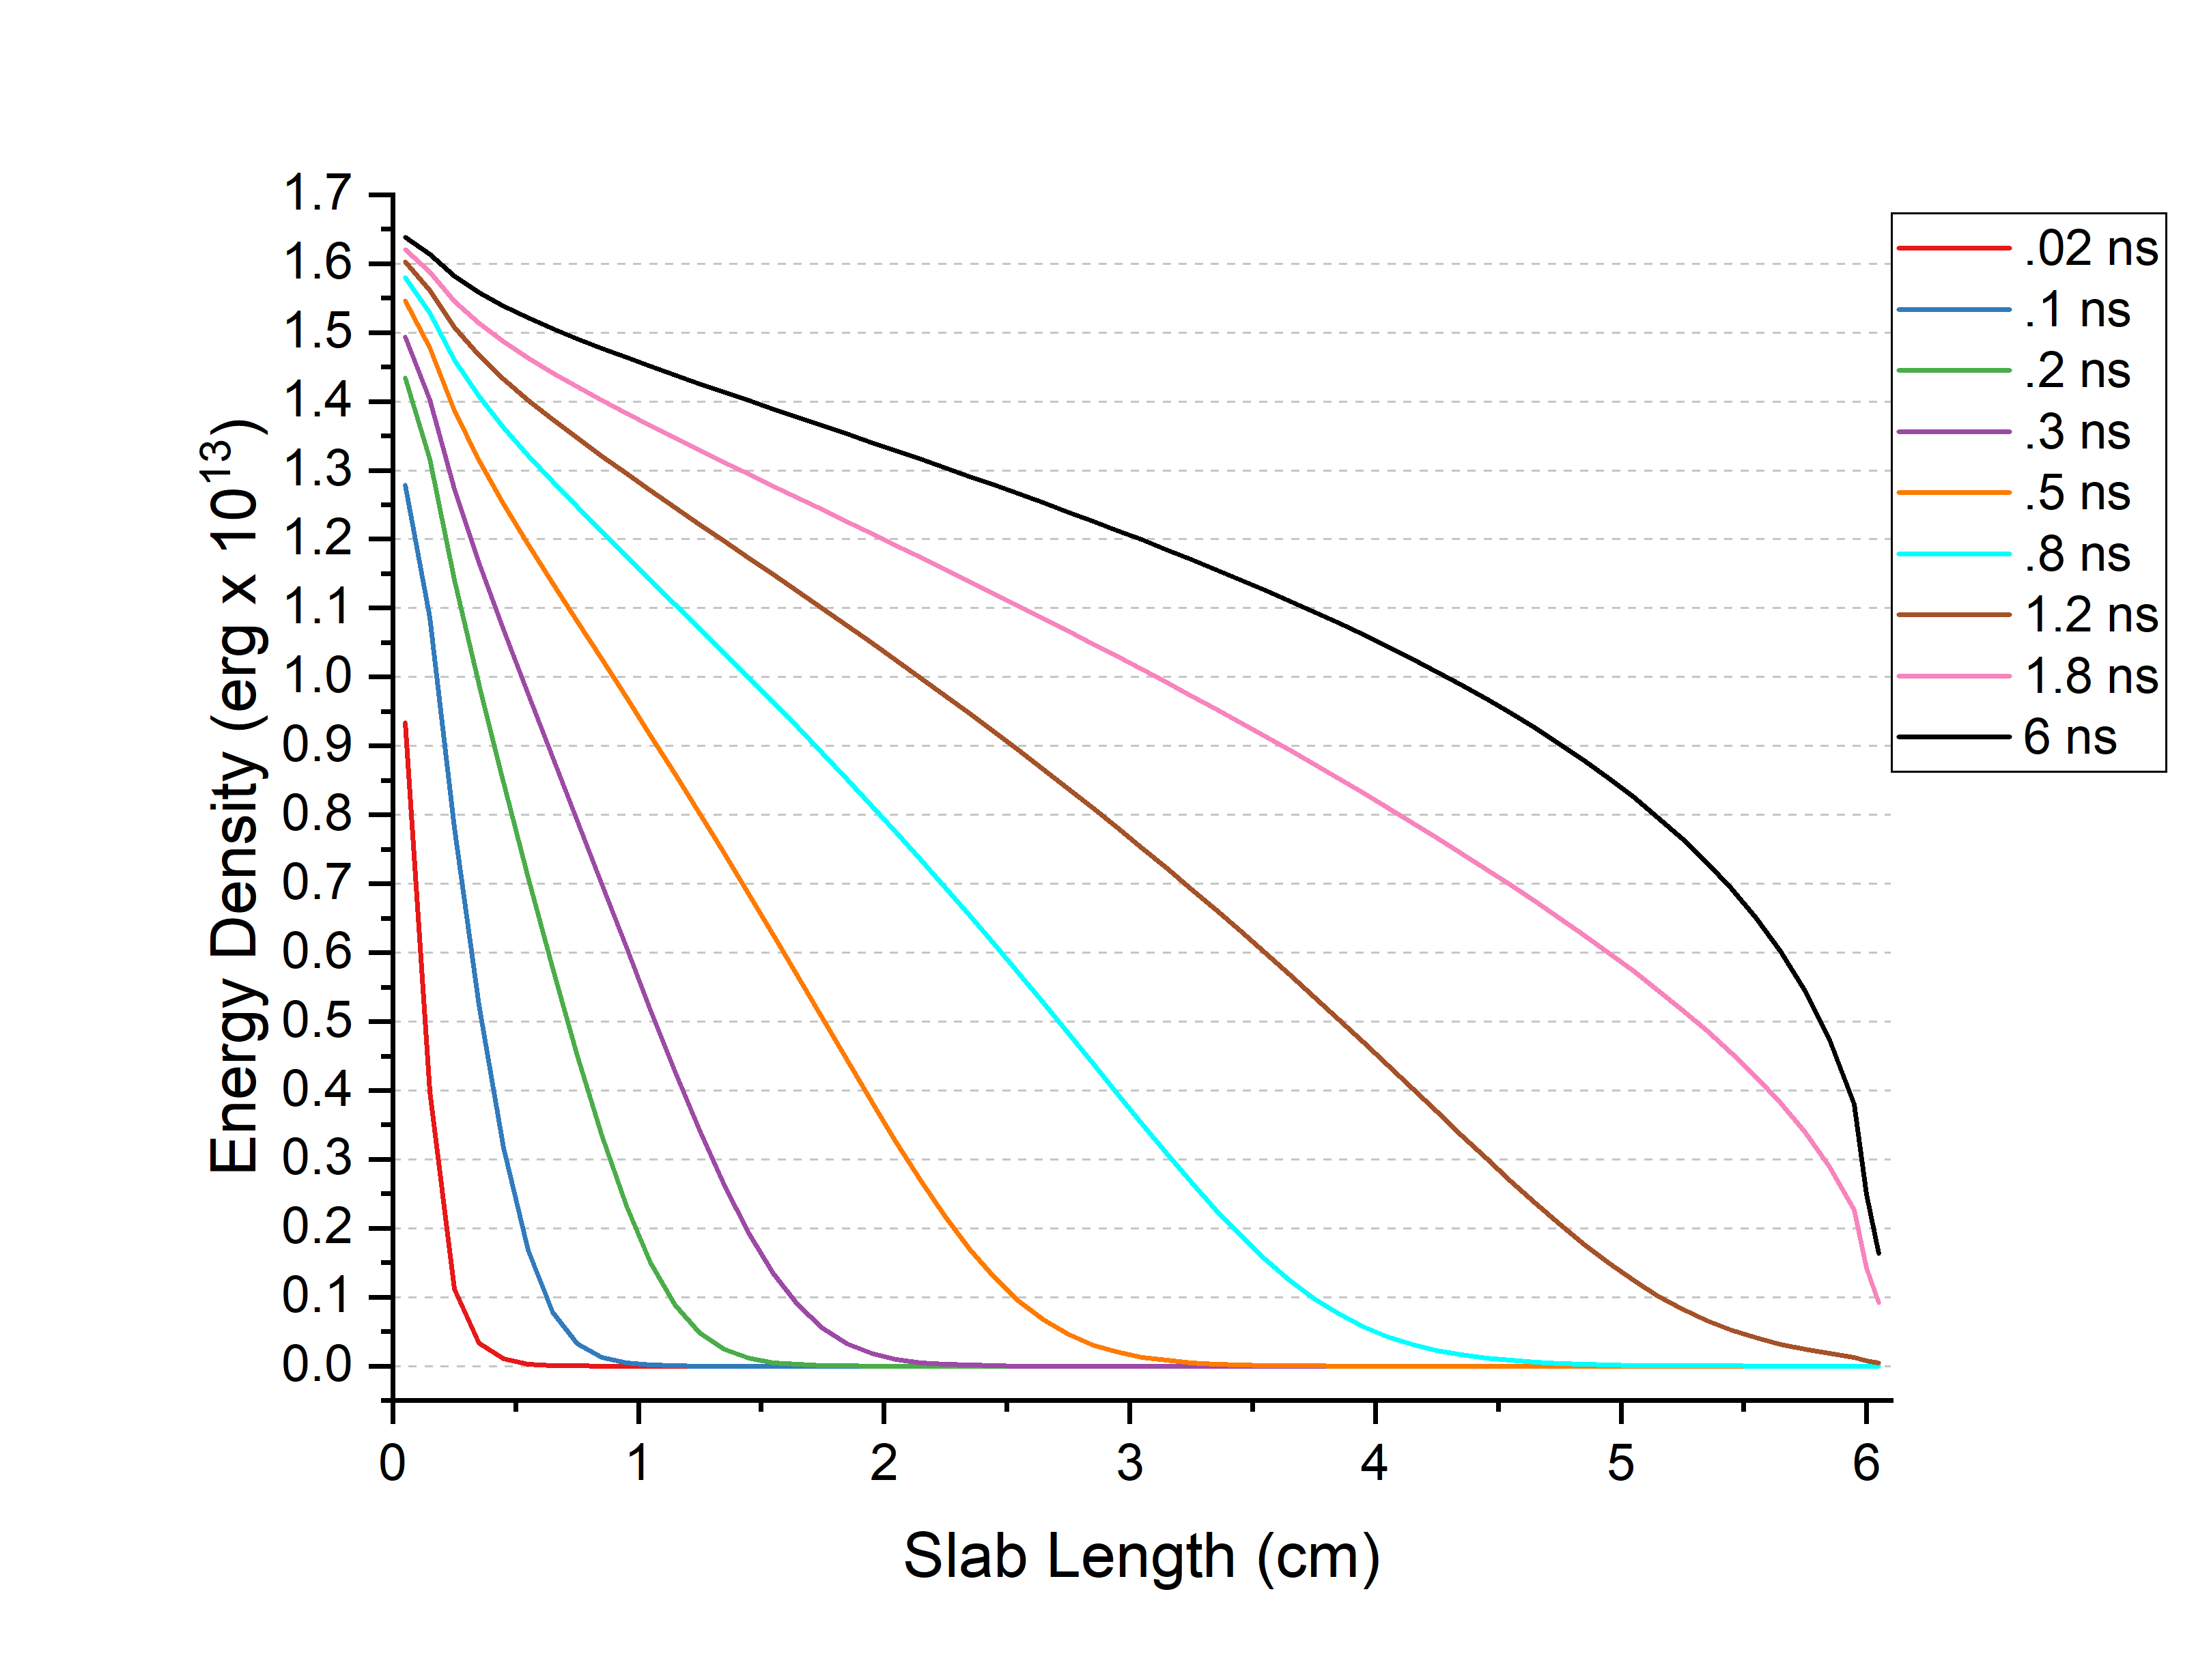
\includegraphics[width=0.5\textwidth]{Eg_g3_cut20_grey.png}}
		\caption{\label{fig:Eg_g3_recomps}
			Low-rank approximations of the group radiation energy density ($E_g^*$) based on the POD for $g=3$ for select time steps}
	\end{figure}
	
	%=================================================================================
	% Eg G8 RECOMP
	\begin{figure}[ht!]
		\centering
		\subfloat[r = 1 \label{subfig:Eg_g8_cut1_grey}]{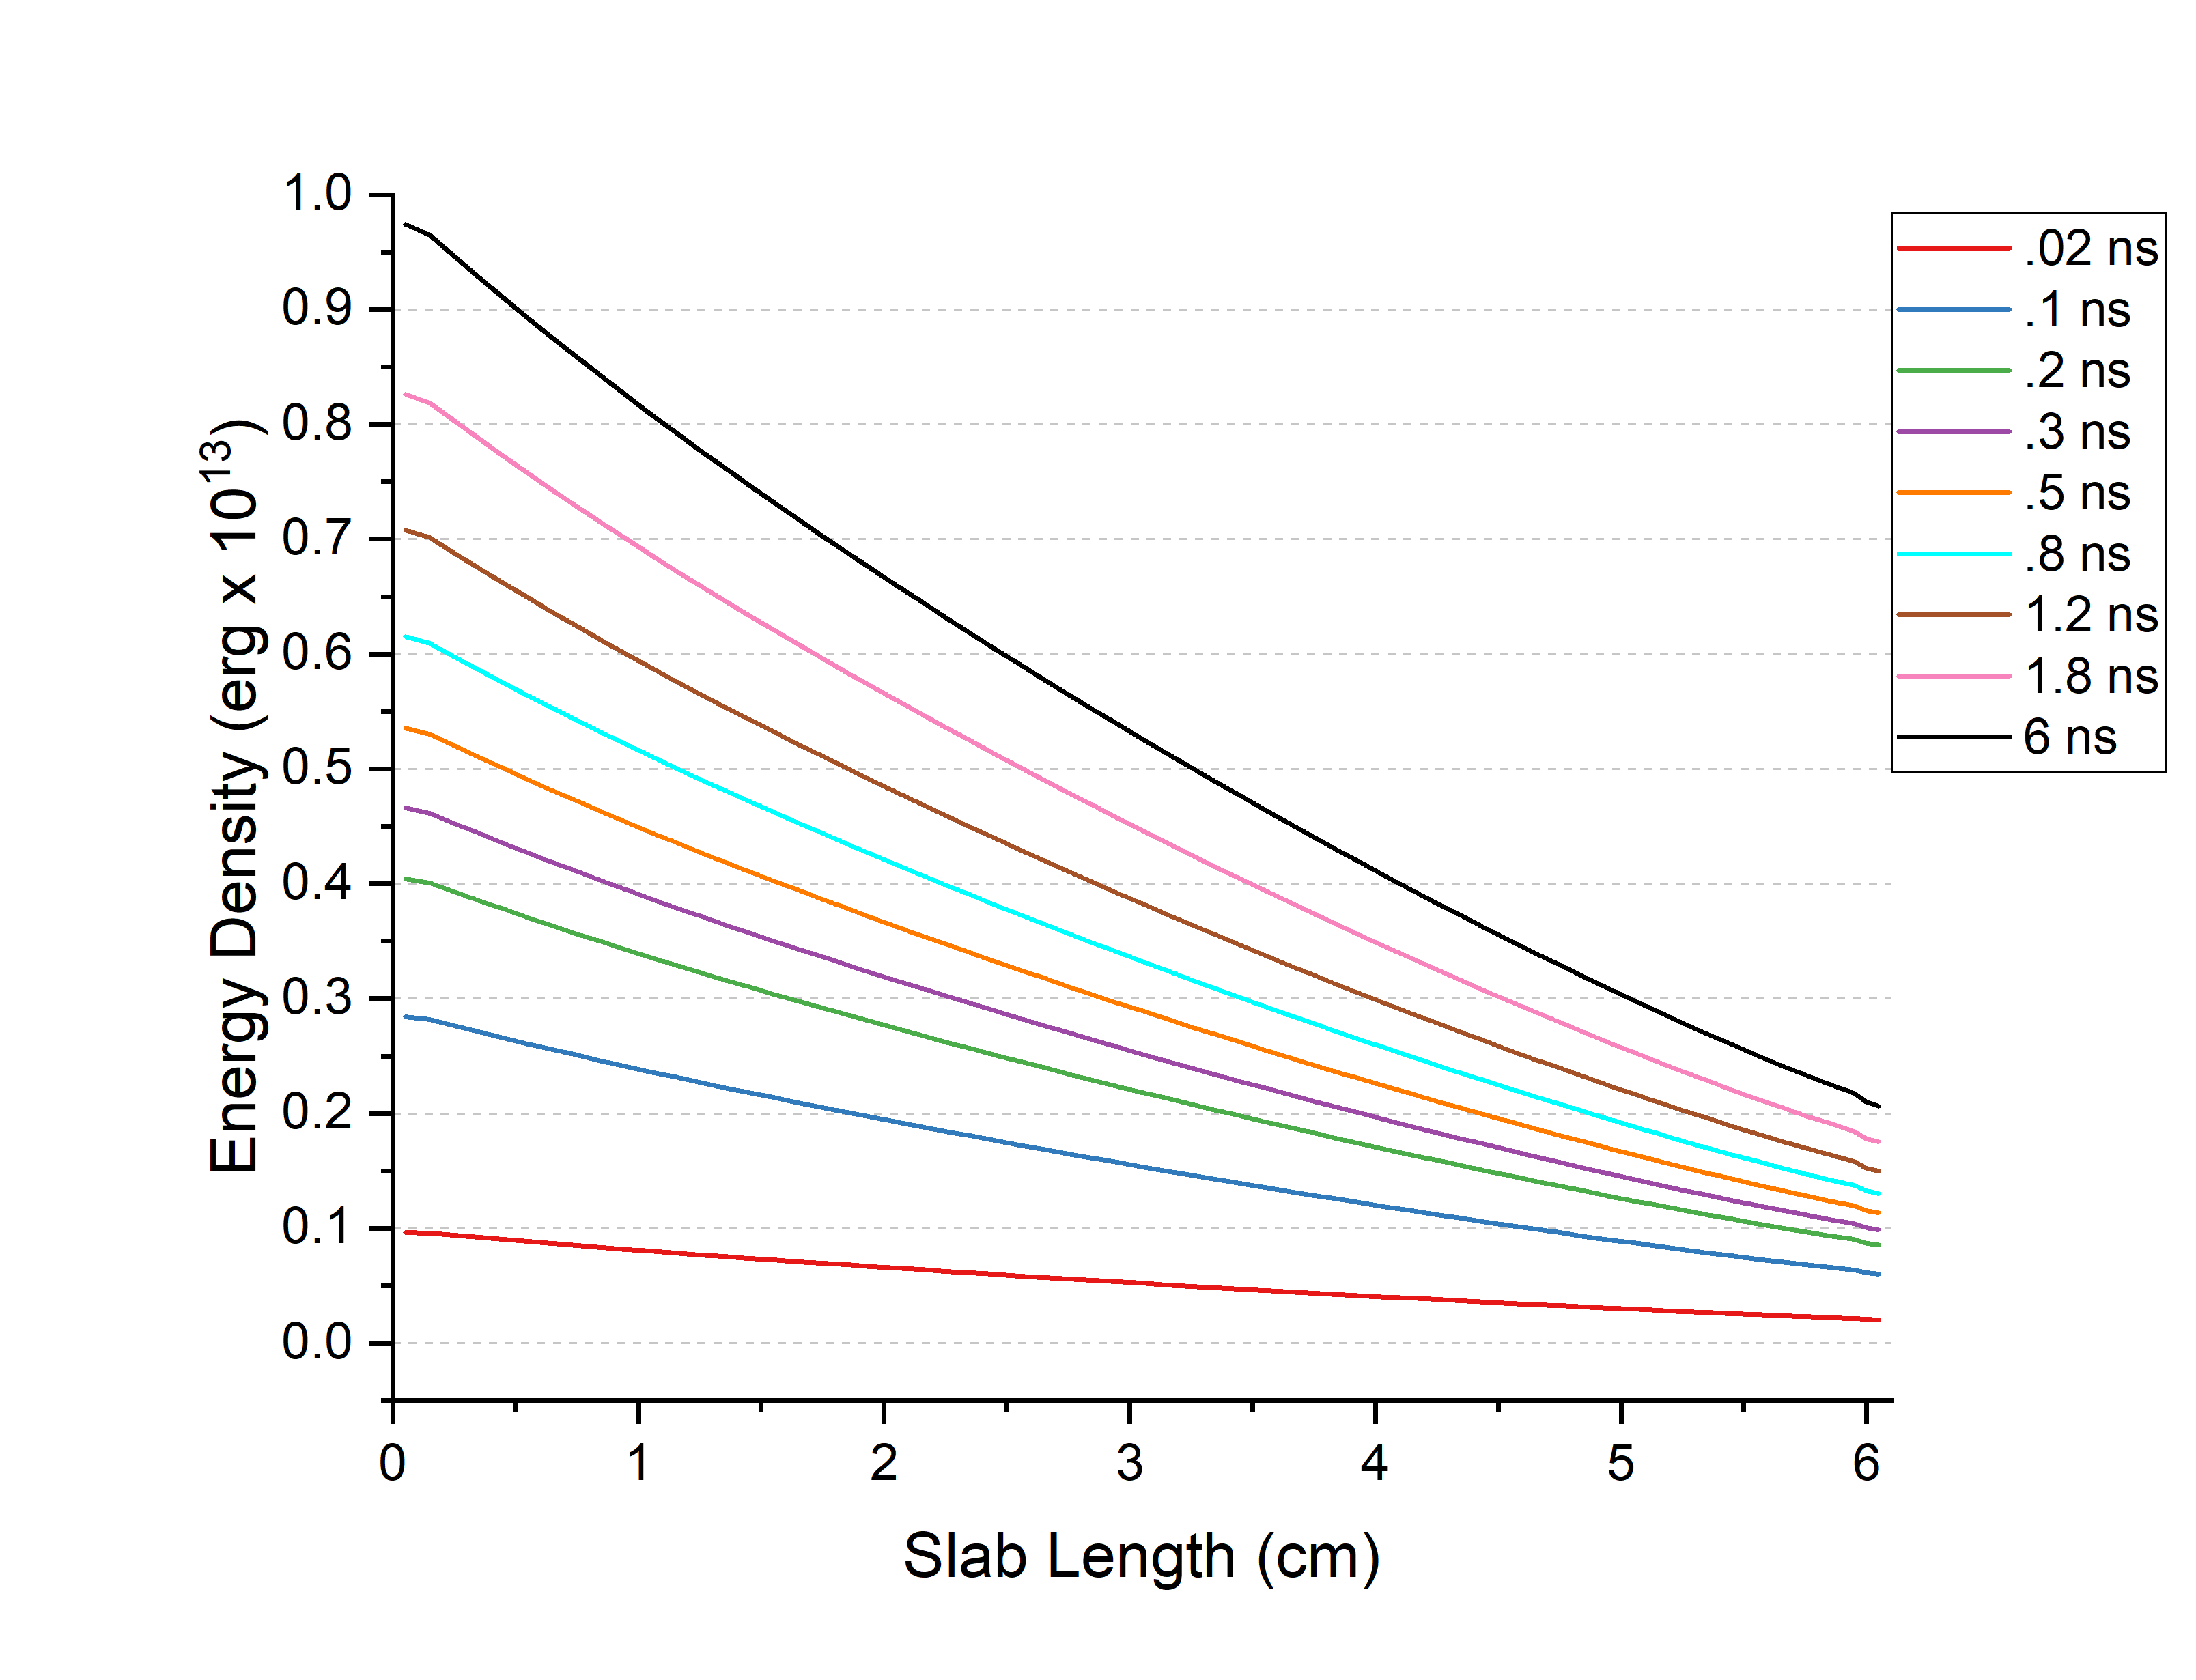
\includegraphics[width=0.5\textwidth]{Eg_g8_cut1_grey.png}}
		\subfloat[r = 2 \label{subfig:Eg_g8_cut2_grey}]{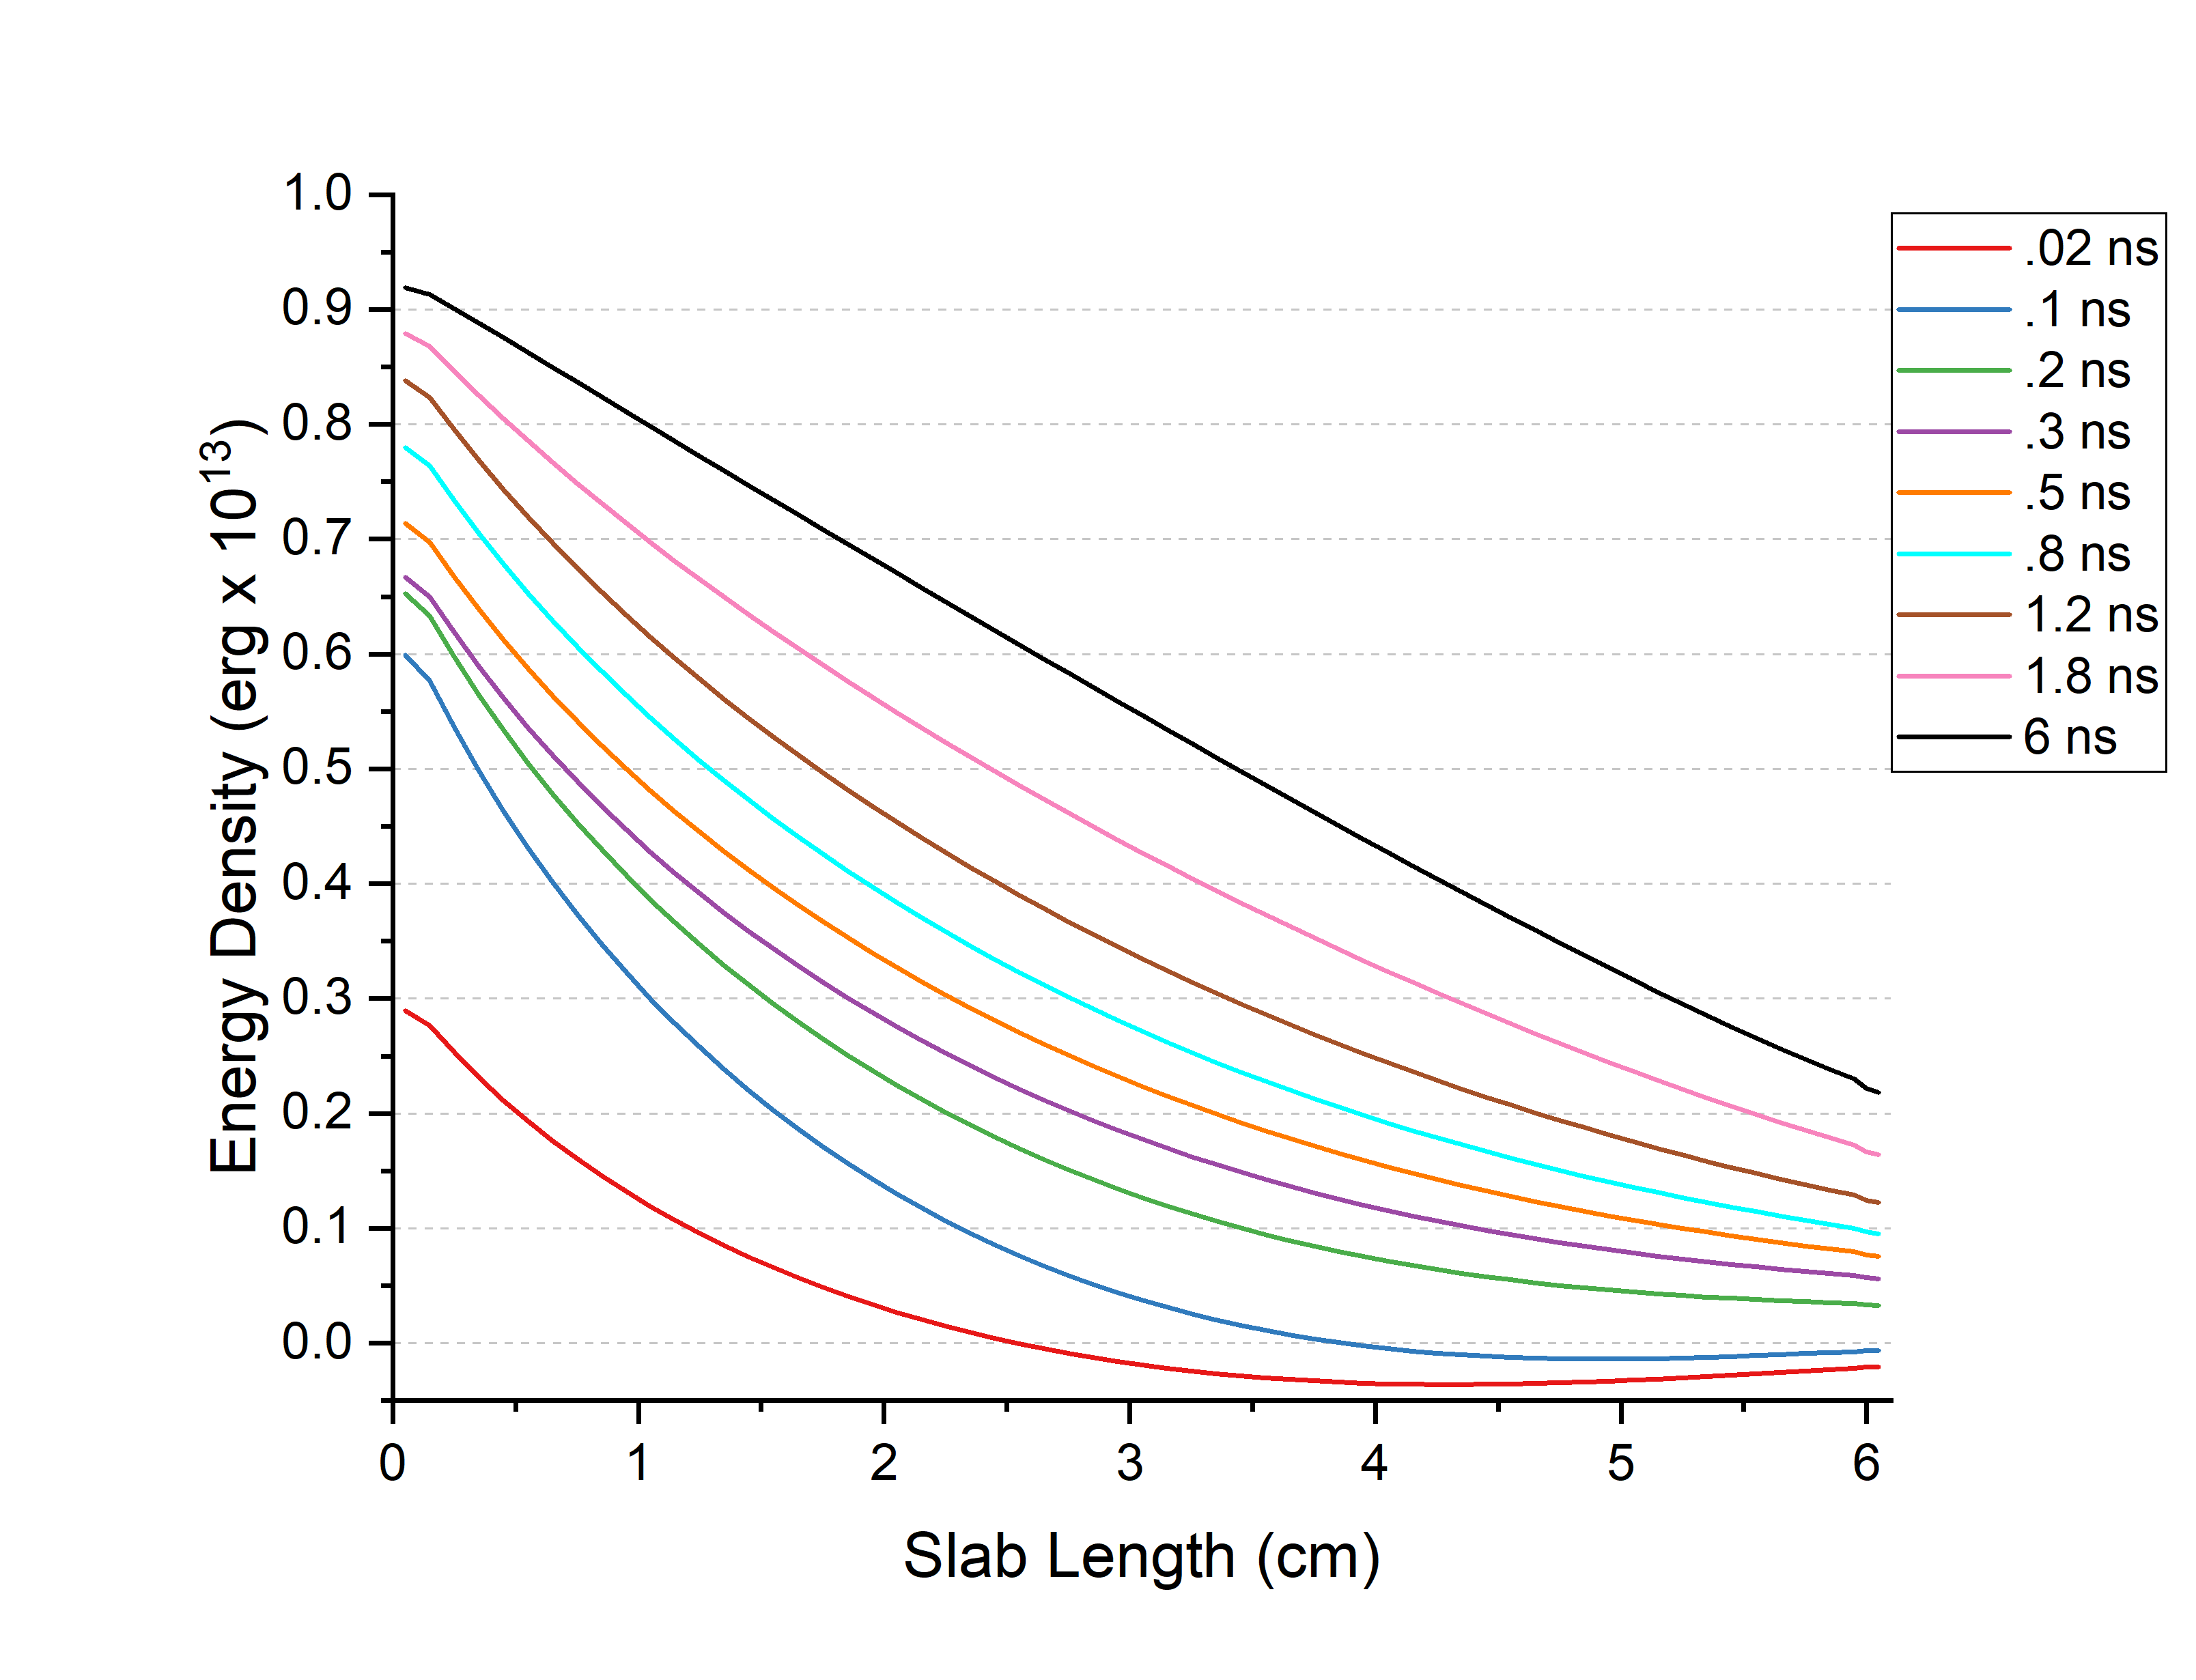
\includegraphics[width=0.5\textwidth]{Eg_g8_cut2_grey.png}}\\
		\subfloat[r = 5 \label{subfig:Eg_g8_cut5_grey}]{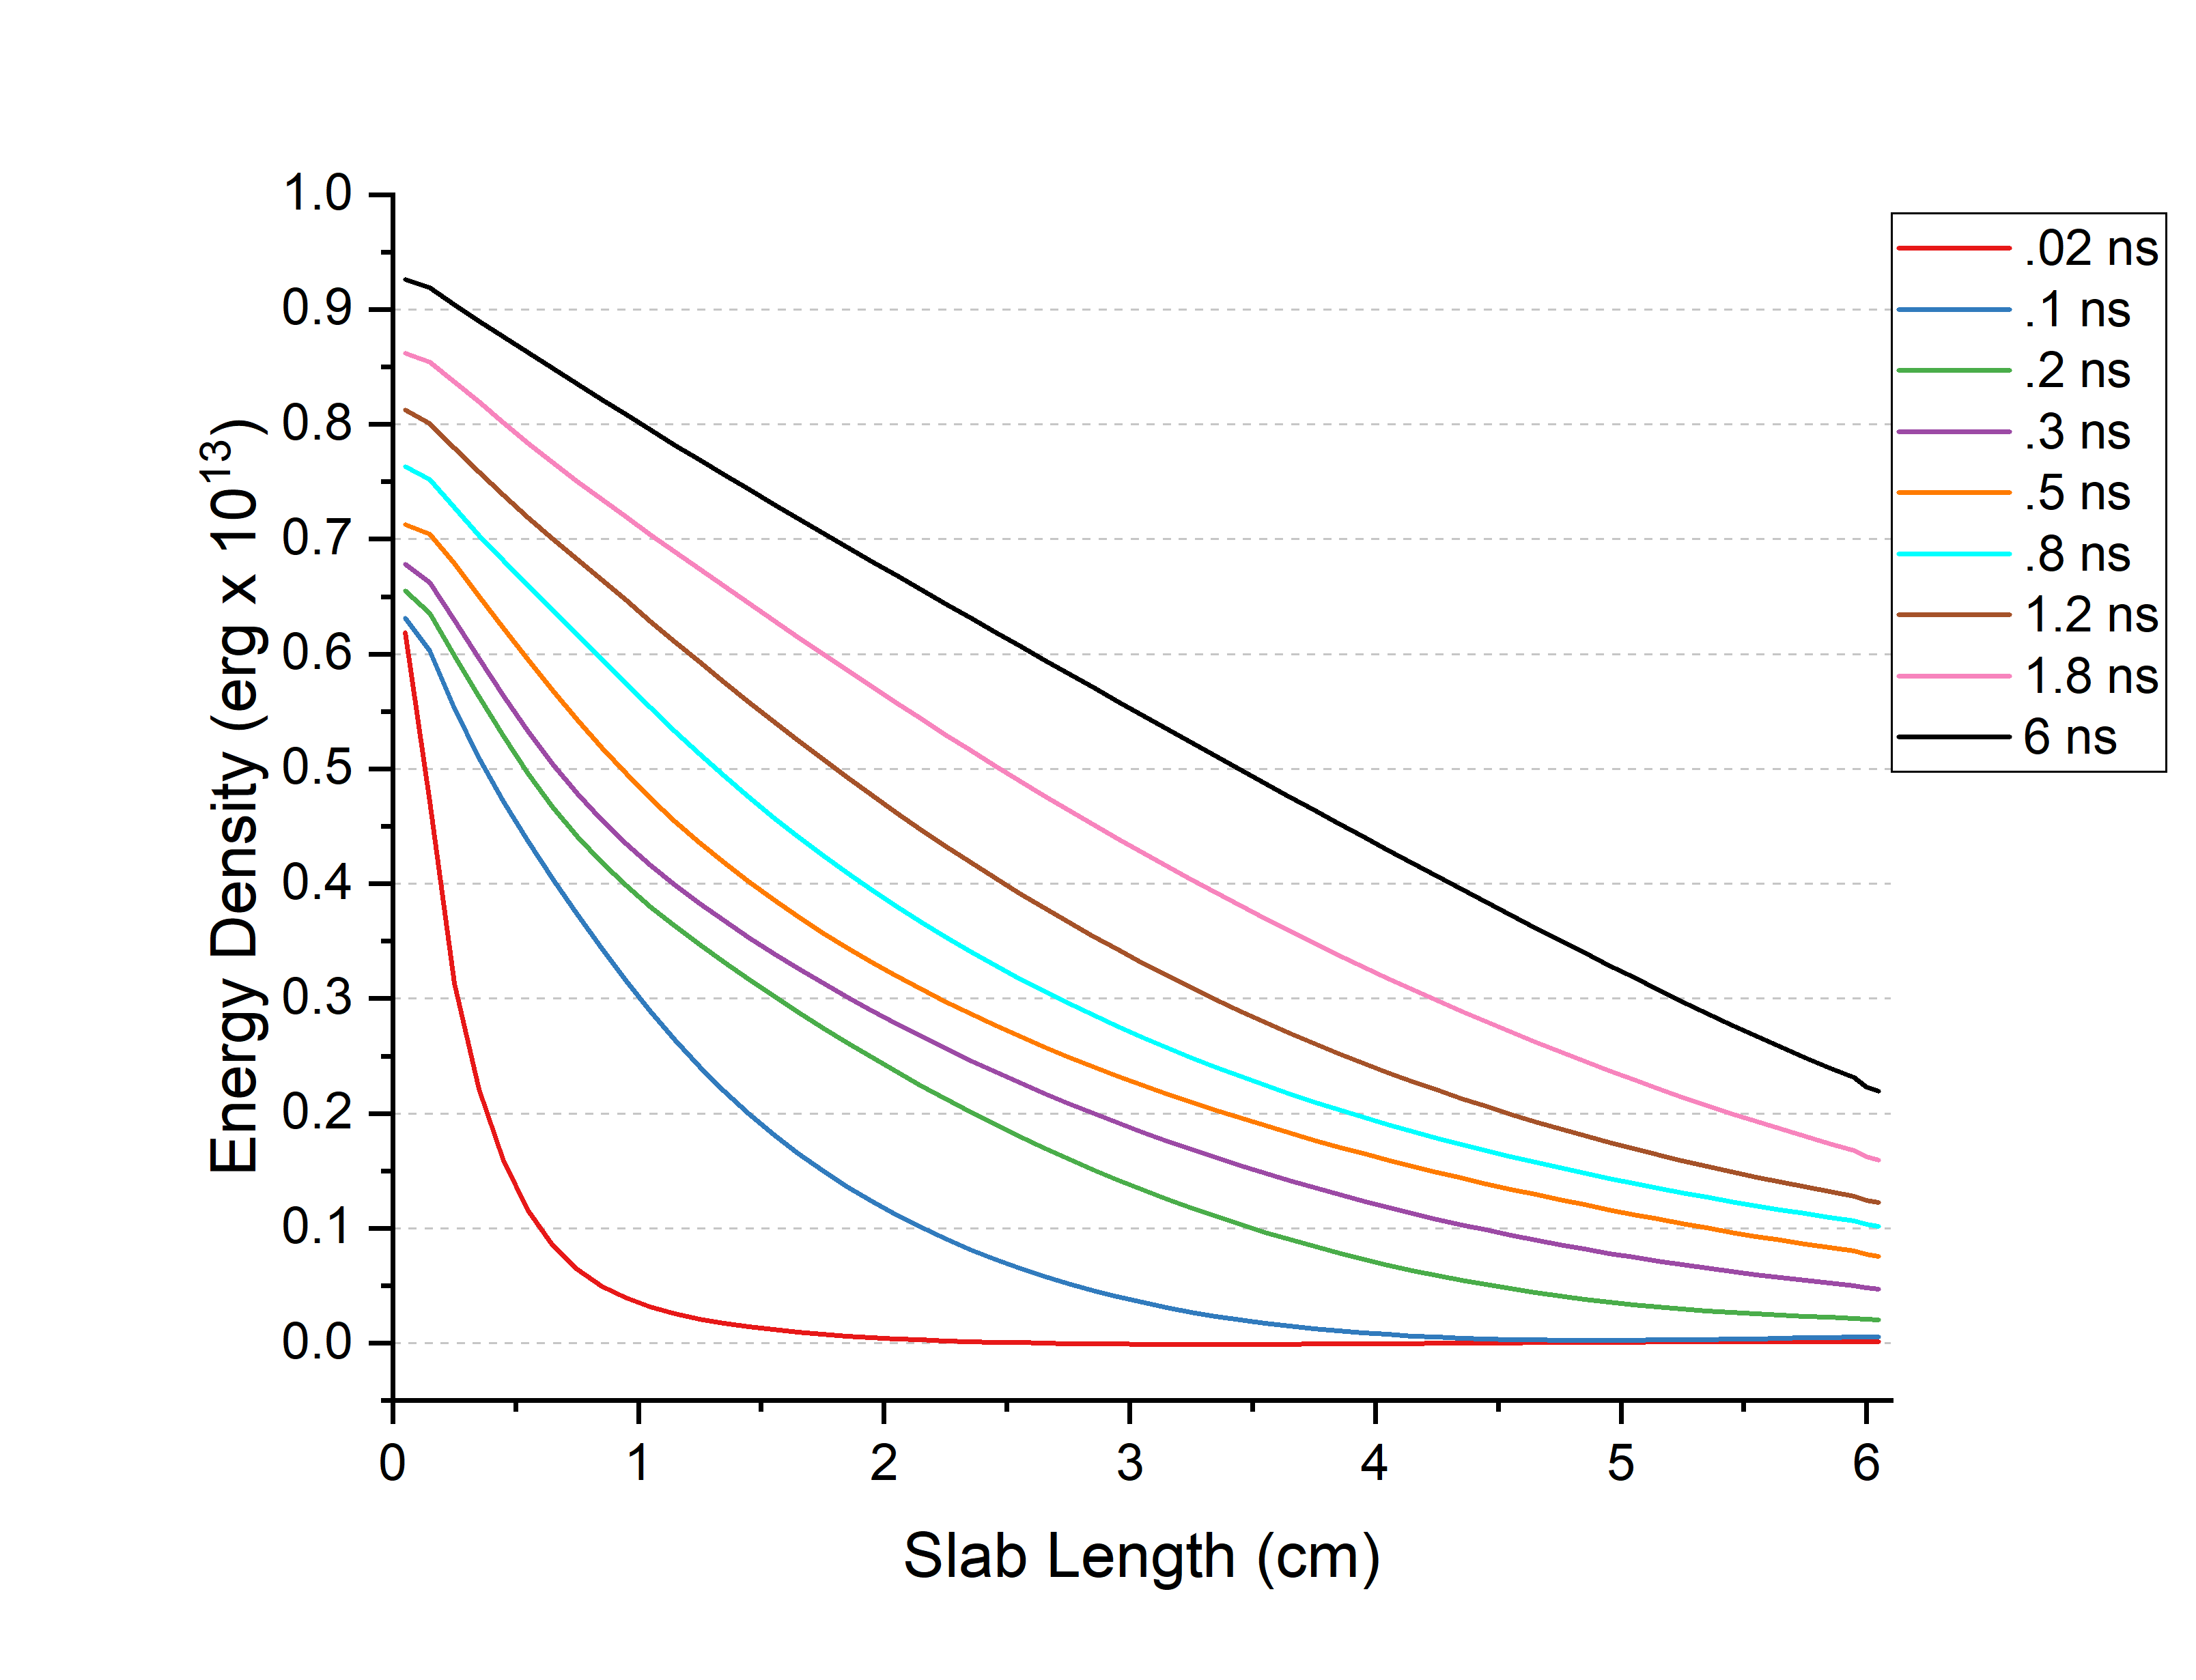
\includegraphics[width=0.5\textwidth]{Eg_g8_cut5_grey.png}}
		\subfloat[r = 10 \label{subfig:Eg_g8_cut10_grey}]{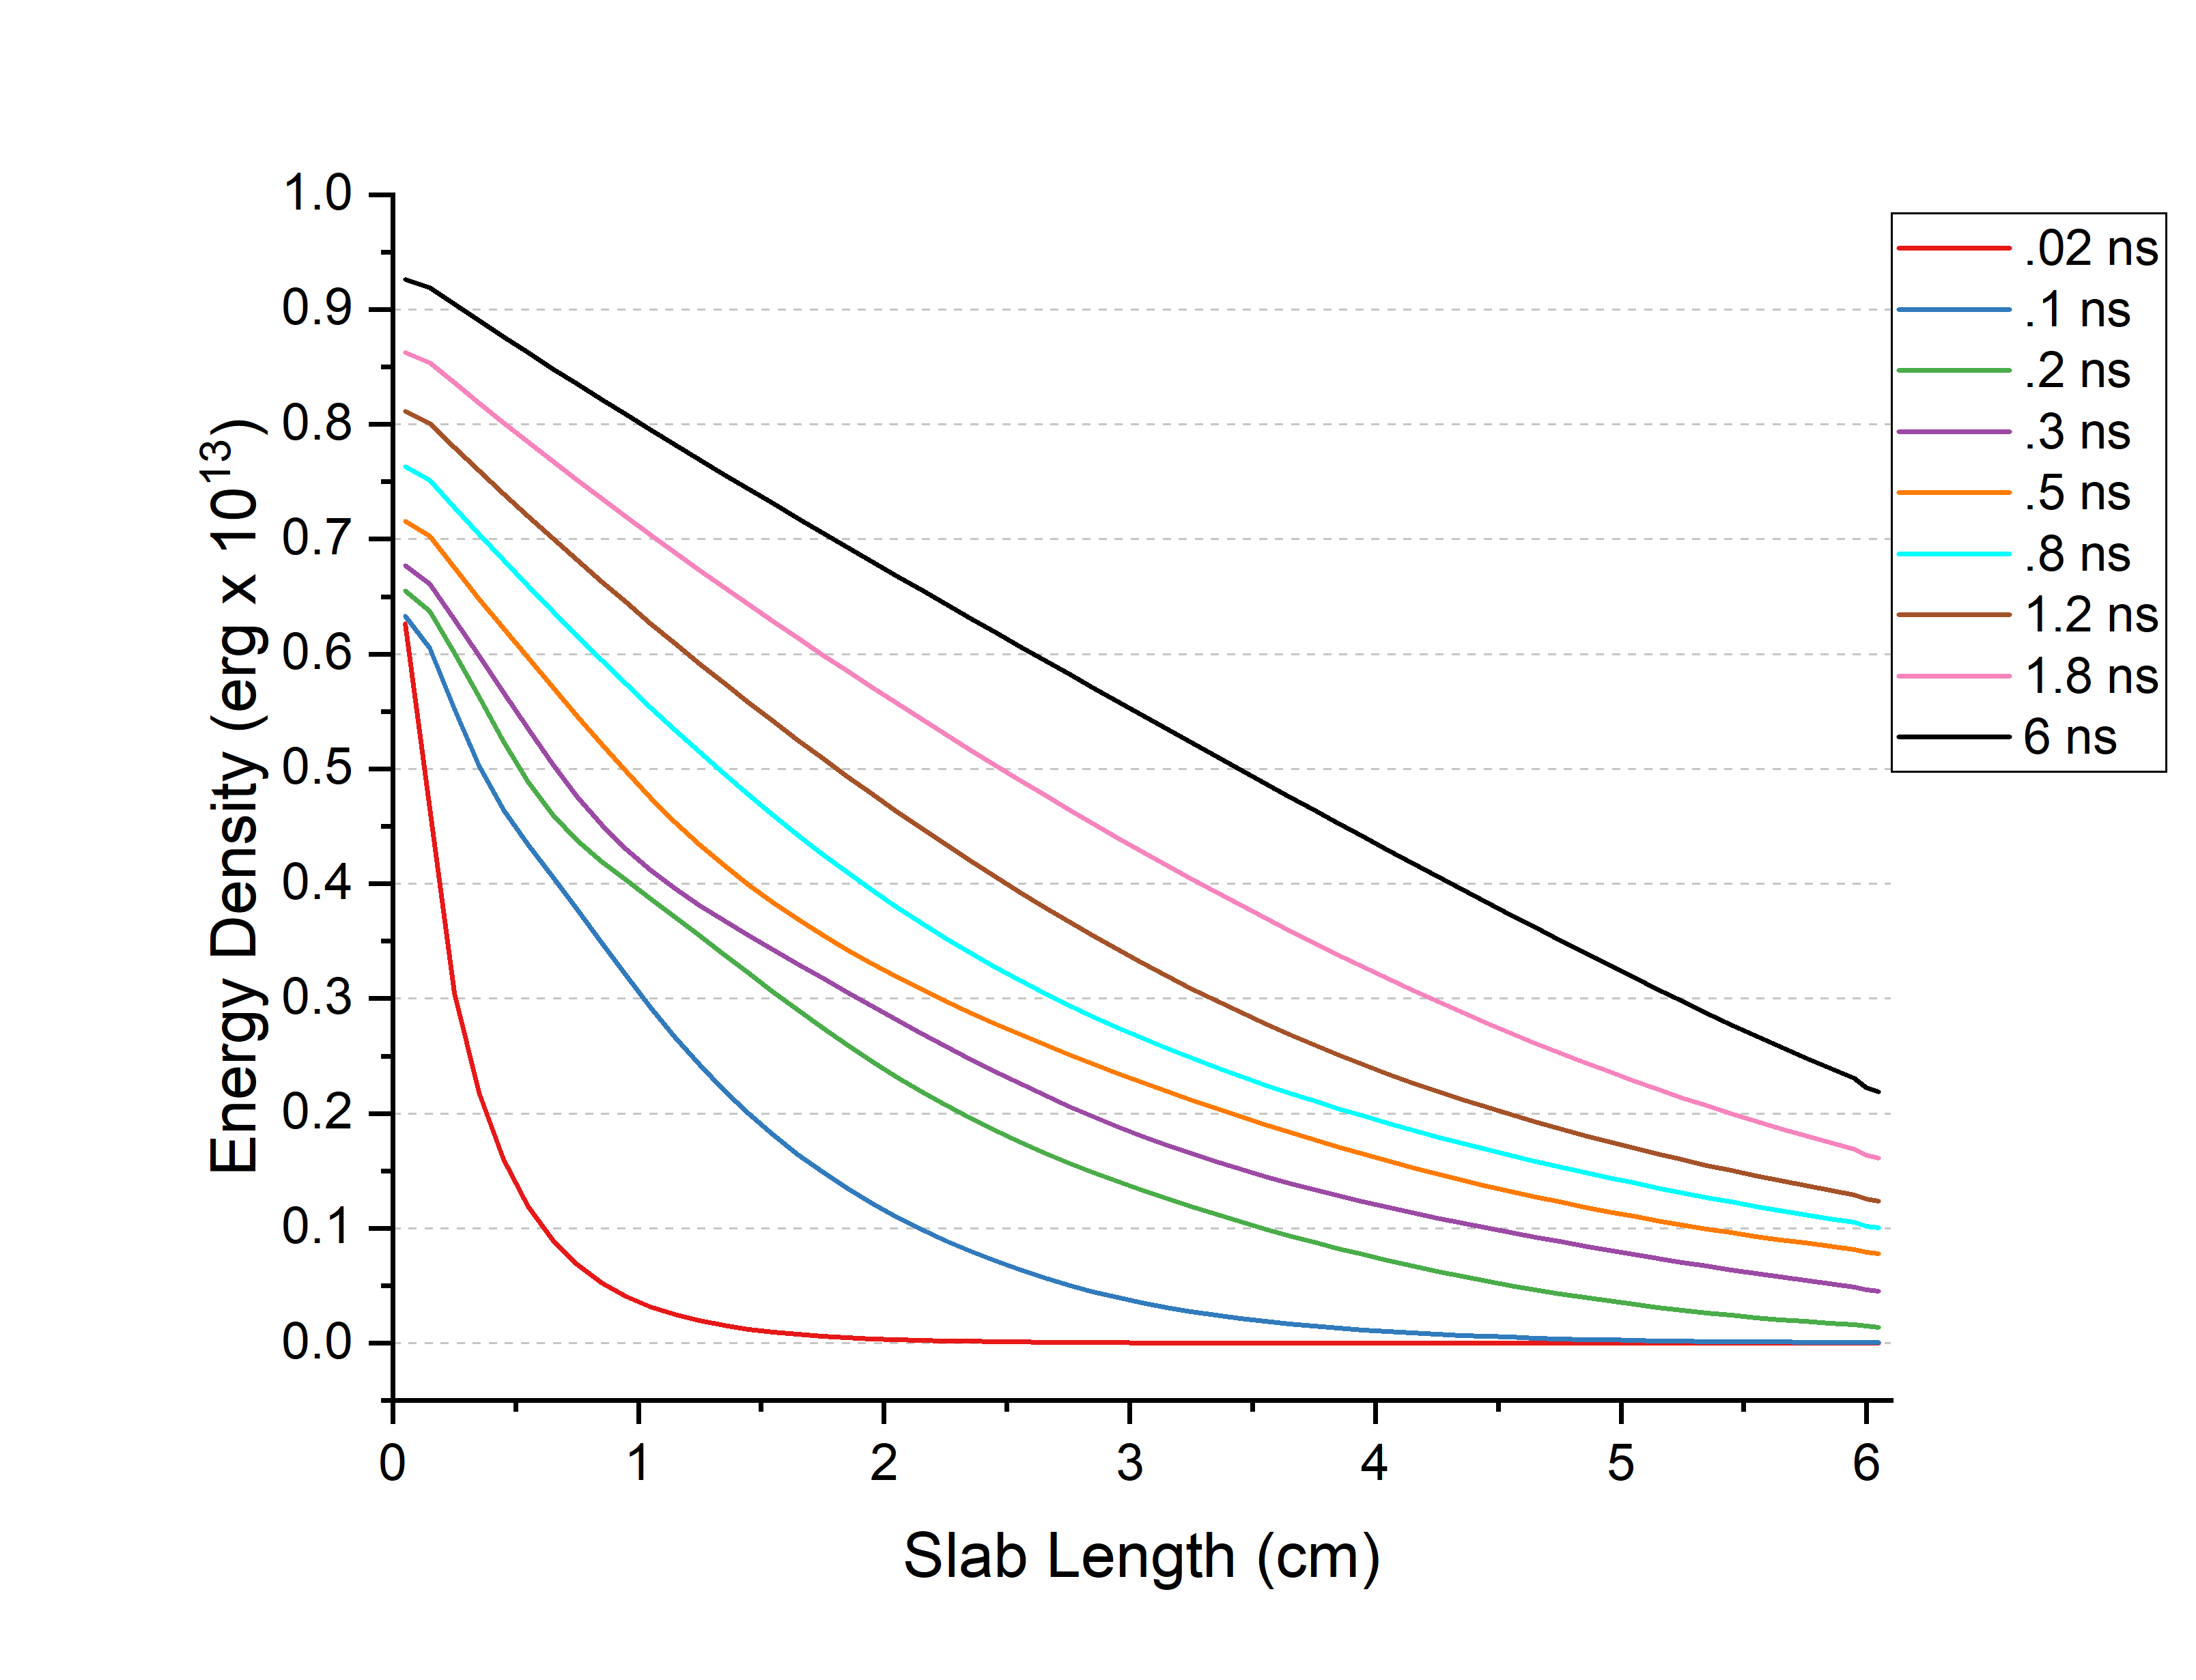
\includegraphics[width=0.5\textwidth]{Eg_g8_cut10_grey.png}}\\
		\subfloat[r = 15 \label{subfig:Eg_g8_cut15_grey}]{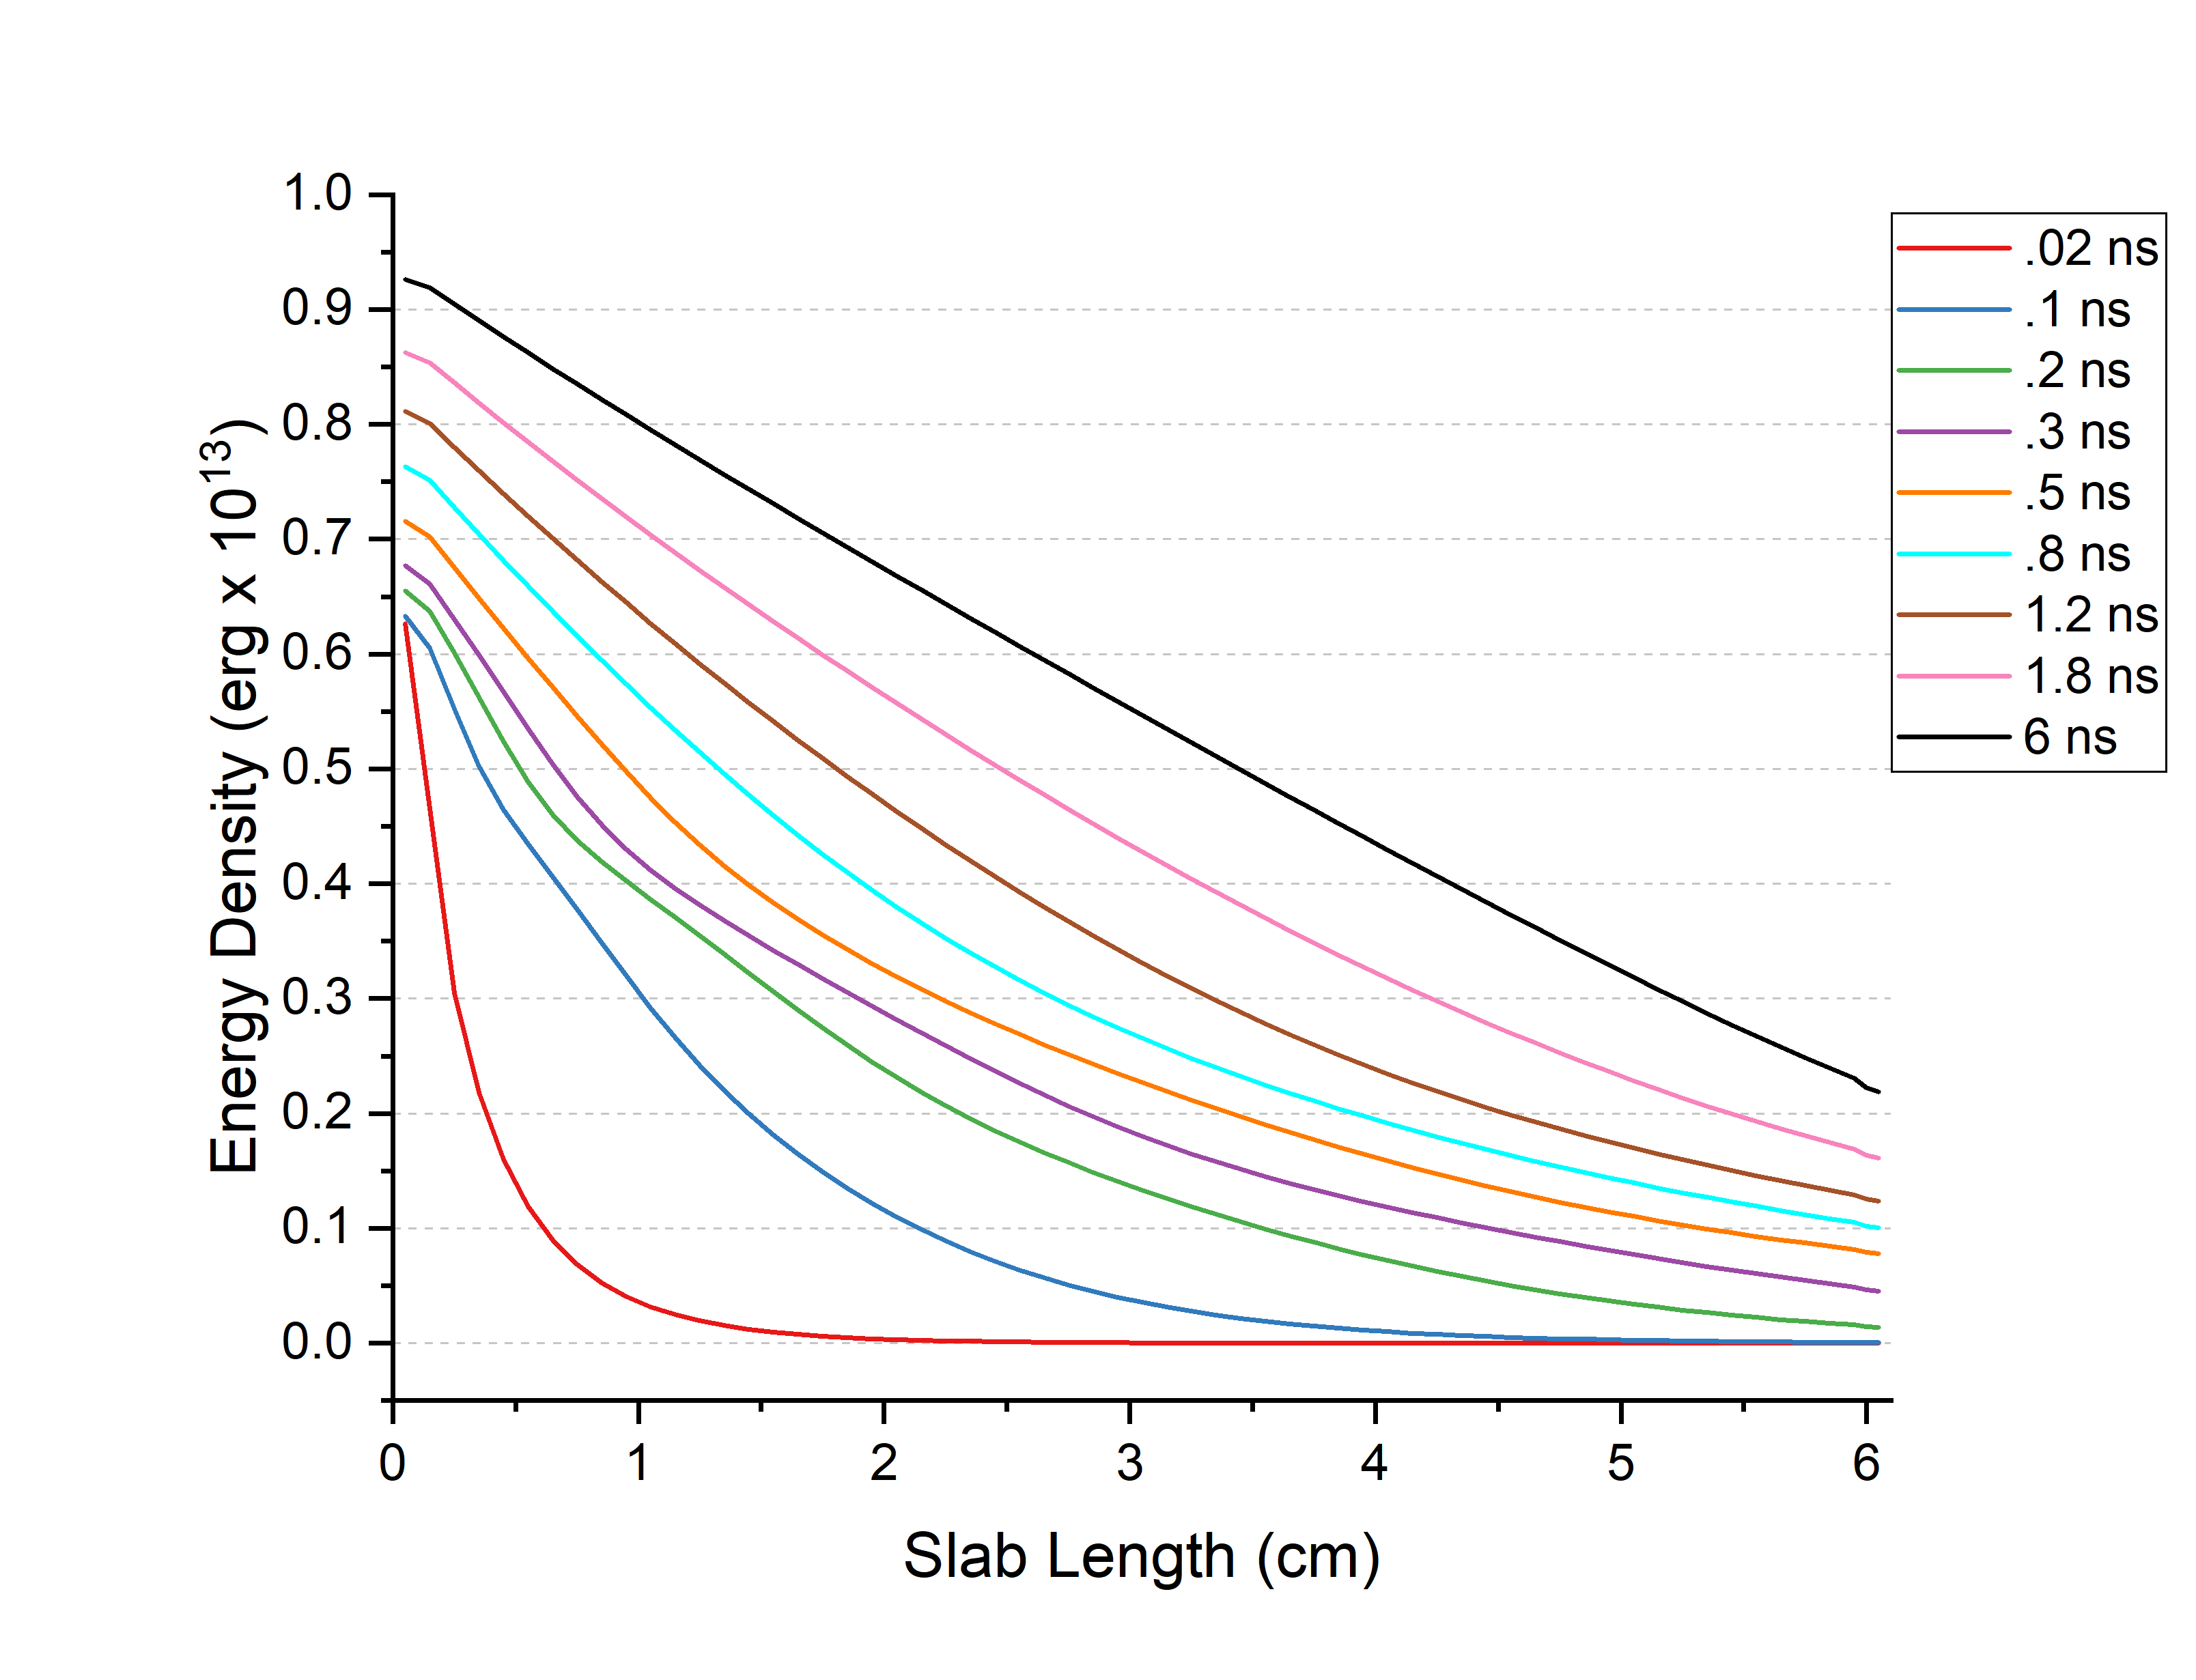
\includegraphics[width=0.5\textwidth]{Eg_g8_cut15_grey.png}}
		\subfloat[r = 20 \label{subfig:Eg_g8_cut20_grey}]{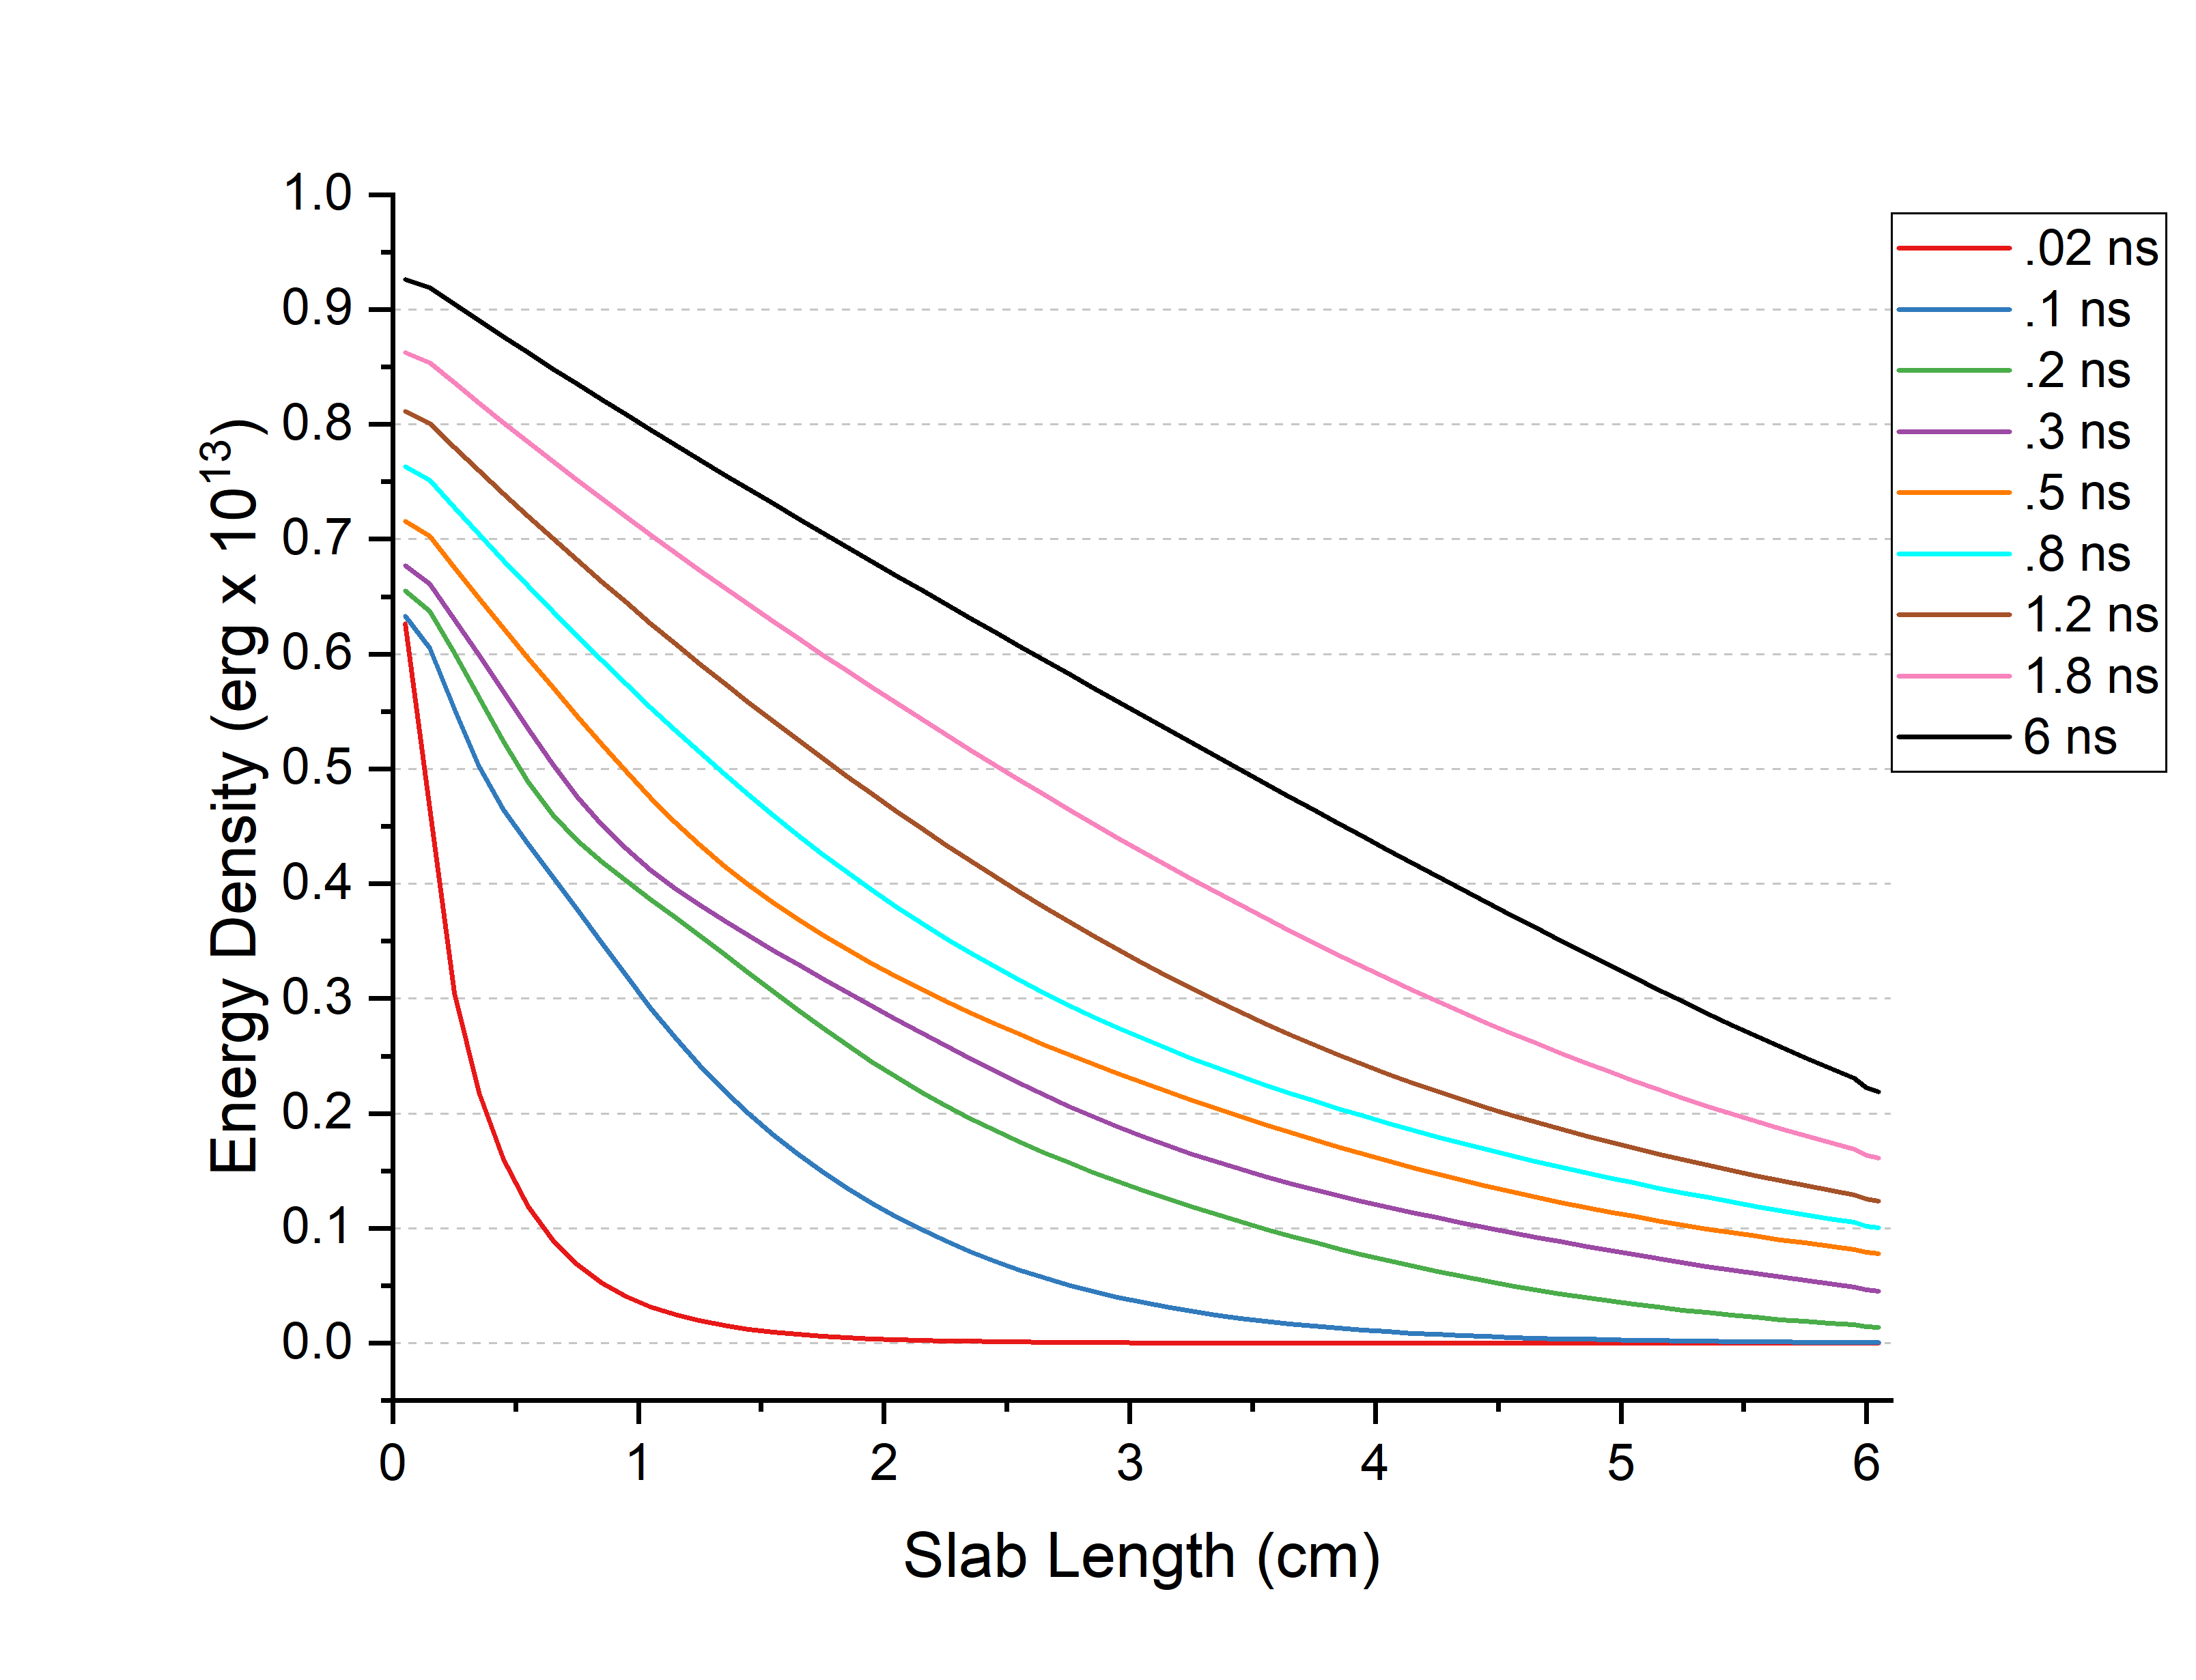
\includegraphics[width=0.5\textwidth]{Eg_g8_cut20_grey.png}}
		\caption{\label{fig:Eg_g8_recomps}
			Low-rank approximations of the group radiation energy density ($E_g^*$) based on the POD for $g=8$ for select time steps}
	\end{figure}

\section[Black-Body Correction for Low-Rank Approximation of Group Energy Densities]{Black-Body Correction for Low-Rank Approximation of \\ Group Energy Densities} \label{bb_cor}
	\ind At low rank, the reduced rank representation of group radiation energy densities was shown to become oscillatory and negative for early times in Sec. \ref{reduced_eg}. This effect of the POD must be considered for the GLOQD-POD ROM, because negative group radiation energy densities have the potential to impact the quality of the ROM solution. To improve the low-rank POD of $E_g$, we introduce a correction which replaces the negative reduced rank radiation energy densities with the black-body spectrum at the material temperature. This kind of spectrum  function does not take into account non-local radiation. In areas dominated by local radiation emitted by the material however, the black-body radiation spectrum is a good approximation of the actual radiation spectrum. As discussed in Sec. \ref{reduced_eg}, the low rank group radiation energy densities become oscillatory and negative in spatial regions where the radiation wave has not reached yet. Since the radiation in these regions is prevalently local the black-body spectrum is a good correction for the low rank radiation energy densities that have become negative.
	
	\ind The GLOQD-POD ROM makes use of this correction when gathering approximate group radiation energy densities from the given databases. To rid the reduced rank radiation energy densities of any artifacts of oscillatory structure, an assumption is made that the radiation wave ends where the energy densities of any given group first becomes negative. The position where the radiation wave ends for group $g$ is $x^{\text{wave}}_{g}$. Thus at each instant of time, all group radiation energy densities in the interval $x\in\brk{x^{\text{wave}}_{g},X}$ are replaced with the black-body spectrum at the material temperature. To calculate the group radiation energy density from the black body spectrum $\pr{E^B_g}$, the group radiation intensity $\ig$ is replaced with the group black-body radiation spectrum $\Bg$ in the definition of the group radiation energy density \eqref{egdef} to yield
	\begin{equation}
		E^B_g = \frac{4\pi}{ c}\Bg\pr{T}.
	\end{equation}
	
	Algorithm \ref{alg:glqd_bg_rom_alg} presents the GLOQD-POD ROM algorithm that corrects reduced rank group radiation energy densities with the black-body spectrum.
	
	\begin{algorithm}[ht!]
		\SetAlgoLined
		\While{$t^n<t^{\text{end}}$}{
			$n=n+1$\\
			$T^{\pr{0}} = T^{n-1}$\\
			$\bfg^* \leftarrow \bA^{f*}_g$, \ \ $\eg^* \leftarrow \bA^{E*}_g$\\
			Find $x^{\text{wave}}_g$ from $\eg^*$
			\While{$\norm{T^{\ell}-T^{\ell-1}} > \tilde{\epsilon}_1\norm{T^{\ell}} + \tilde{\epsilon}_2, \ \ \norm{\eb^{\ell}-\eb^{\ell-1}} > \tilde{\epsilon}_1\norm{\eb^{\ell}} + \tilde{\epsilon}_2 $}{
				$\ell=\ell+1$
				Update opacities $\kapg\pr{T^{\ell}}$\\
				Update $4\pi c\Bg\pr{T^\ell} \ra \eg^*$ for $x\in\brk{x^{\text{wave}}_{g},X}$\\
				Update group radiation fluxes $\bFg^*$ with MLOQD-POD Eqs. \eqref{mlqd_pod_eqs}\\
				Compute grey quantities $\kapeb^{*,\ell}$, $\kapbb^{\ell}$, $\kaprb^{*,\ell}$, $\bfb^{*,\ell}$, $\etab^{*,\ell}$\\
				Solve coupled GLOQD-POD and MEB Eqs. \eqref{glqd_pod_eqs} for $\eb^{\ell}$, $\bFb^{\ell}$, $T^{\ell}$
			}
			$T^n \leftarrow T^\ell$
		}
		\caption{Nonlinear QD Iterative Scheme for the GLOQD-POD ROM using reduced rank databases of group QD factors $\bA^{f*}_g$ and group radiation energy densities $\bA^{E*}_g$ corrected with black-body spectrum \label{alg:glqd_bg_rom_alg}}
	\end{algorithm}

\section{Numerical Results of the GLOQD-POD ROM} \label{sec:gloqd-pod_res}
	\ind To quantify the accuracy of the GLOQD-POD ROM, the F-C test described in Ch. \ref{chap-three} is used. The problem is solved over $0 \le t  \le 6$ ns using  the time step $\Delta t=2 \times 10^{-2}$ ns. Approximate GLOQD-POD ROMs for this TRT problem are defined using different reduced rank representations of the reference group QD factors and radiation energy densities. Singular value relative cutoff criteria of $\varepsilon_\sigma = 10^{-1}, 10^{-2}, \dots 10^{-12}$ are used. To isolate the effects of using reduced rank forms of the group QD factors and radiation energy densities separately, the reference transport values of certain quantities that have not been decomposed with the SVD will be used in some instances.
	
	\ind Figure \ref{fig:ref_errs_inf_grey} presents the relative error of the solution of these ROMs compared to the reference MLQD solution in the $\infty$-norm at every instant of time. Figs. \ref{subfig:refcase_Temp_rel_inf_fg_grey} and \ref{subfig:refcase_E_rel_inf_fg_grey} show the error of the GLOQD-POD ROM when only using reduced rank forms of the reference QD factors and the transport reference energy densities. Figs. \ref{subfig:refcase_Temp_rel_inf_Eg_grey} and \ref{subfig:refcase_E_rel_inf_Eg_grey} show the error of the  GLOQD-POD ROM when only using reduced rank forms of the reference energy densities and the transport reference QD factors. Figs. \ref{subfig:refcase_Temp_rel_inf_E-fg_grey} and \ref{subfig:refcase_E_rel_inf_E-fg_grey} show the error of the  GLOQD-POD ROM when using reduced rank forms of both the reference energy densities and QD factors. When only using the reduced rank form of the QD factors, the resulting errors are similar to those seen for the MLOQD-POD ROM and when $\varepsilon_\sigma = 10^{-12}$ the reference solution is fully recreated since the error matches the convergence level of the problem $\pr{\epsilon_T=\epsilon_E=10^{-12}}$. While using the reduced rank form of the group radiation energy densities the error is larger and the reference solution is not reproduced when using the full rank representation. The error tends to be high for early times of the problem, significantly being reduced during the interval $0\leq t\leq 5$ ns and then slowly decreasing as the problem progresses. Note that for early times the errors for all $\varepsilon_\sigma$ cluster in two distinct groups, $10^{-1}\leq \varepsilon_\sigma \leq 10^{-7}$ and $10^{-8}\leq \varepsilon_\sigma \leq 10^{-12}$. This is attributed to the large gap seen between the singular value plateaus of groups 3 and 4 in Fig. \ref{subfig:EG_Svals_grey}. The vertical axis of Fig. \ref{subfig:EG_Svals_grey} is equivalent to $\varepsilon_\sigma$, and upon inspection, for $\varepsilon_\sigma\leq 10^{-7}$ the POD with no more than half of its terms of expansion is used for all groups $g>3$. When $\varepsilon_\sigma = 10^{-8}$, groups $g>3$ become full rank and groups $4\leq g \leq 6$ nearly double in rank.
	
	\ind To study the source of the high error observed while using reduced rank group radiation energy densities, the error over the spatial domain of the test problem is examined. Fig. \ref{fig:ref_errs_domain_grey} shows the error in the GLOQD-POD ROM solution relative to the reference solution using the full rank representation of the radiation energy densities and the reference QD factors. The error is only shown for select early times where the highest error resides. Comparing Fig. \ref{fig:ref_errs_domain_grey} with the reference solution in Fig. \ref{fig:ref_sols} the error can be related to a position relative to the radiation wave. This demonstrates the elevated errors at early times to occur in front or before the radiation wave front where only background radiation is present. These areas are comprised entirely by non-local radiation and the radiation energy densities and temperatures present there are extremely small. Thus even though the relative error shown for these regions is high, the absolute error is very small. Fig. \ref{fig:ref_errs_domain_grey} shows that the actual radiation wave is found with errors under $10^{-8}$ for all times.
	
	%=================================================================================
	% TEST PROBLEM ERRORS
	\begin{figure}[ht!]
		\centering
		\subfloat[reduced rank QD factor temperature error \label{subfig:refcase_Temp_rel_inf_fg_grey}]{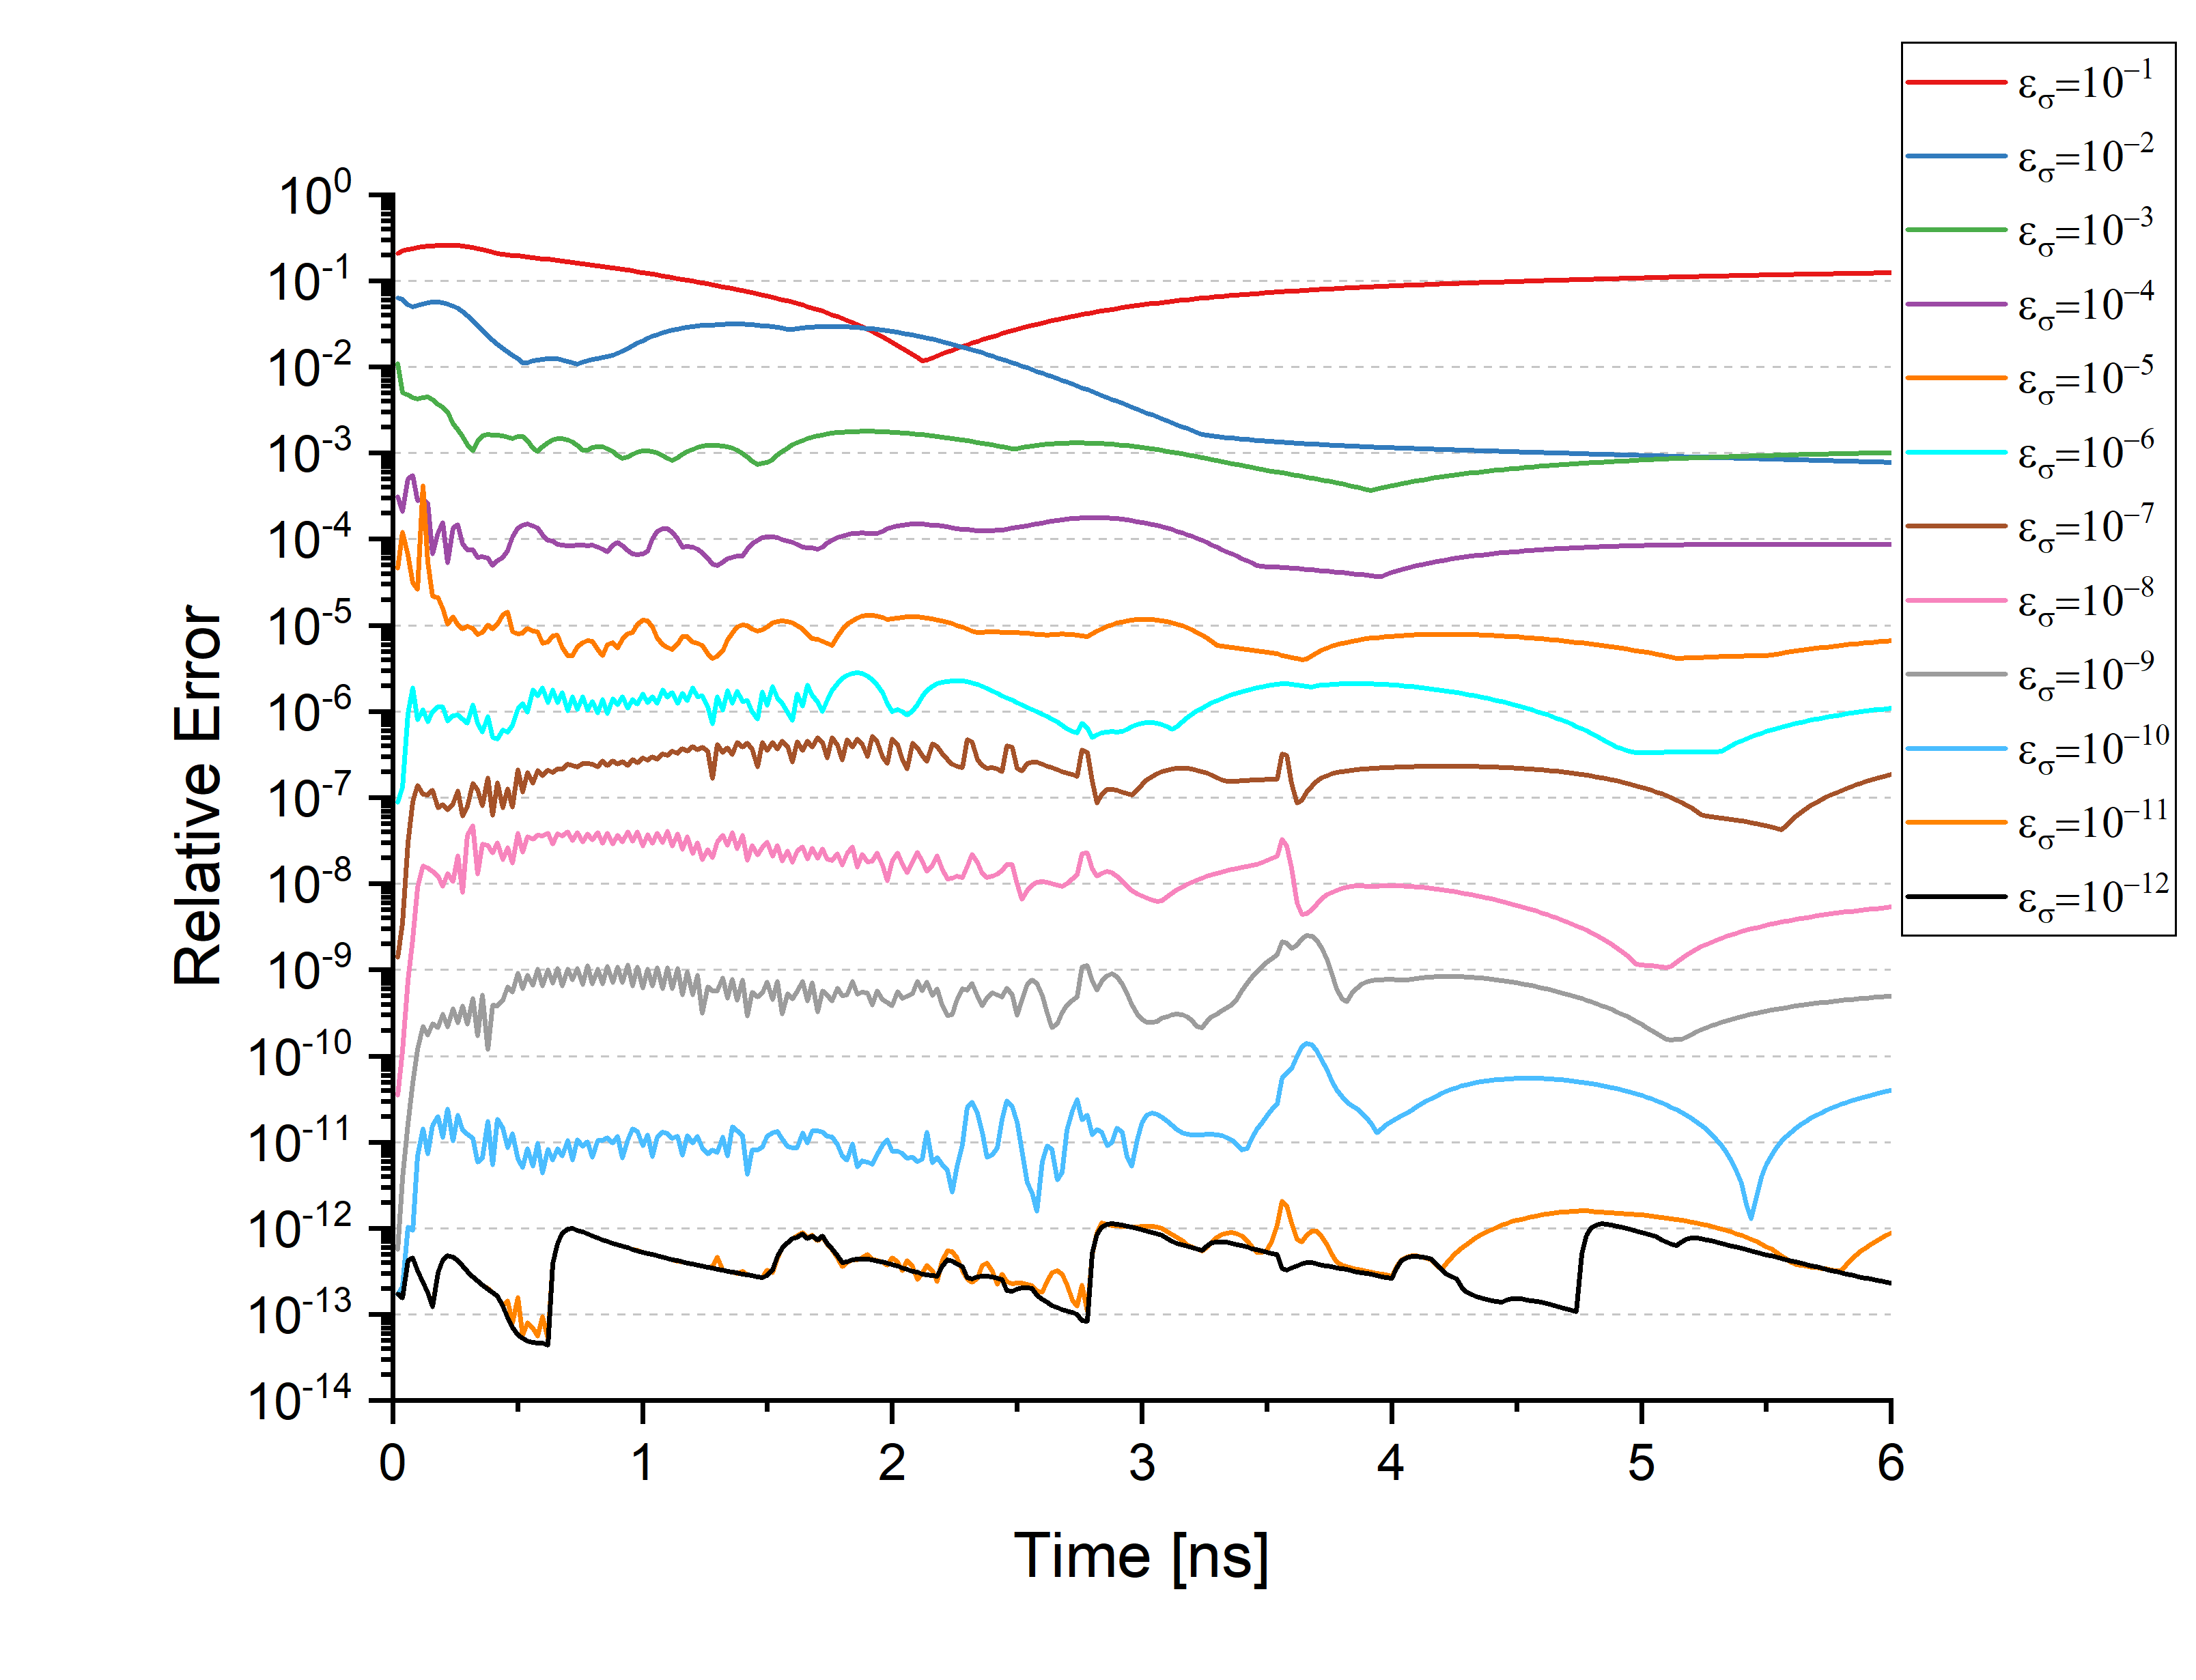
\includegraphics[width=0.475\textwidth]{refcase_Temp_rel_inf_fg_grey_bg.png}}
		\subfloat[reduced rank QD factor total energy density error \label{subfig:refcase_E_rel_inf_fg_grey}]{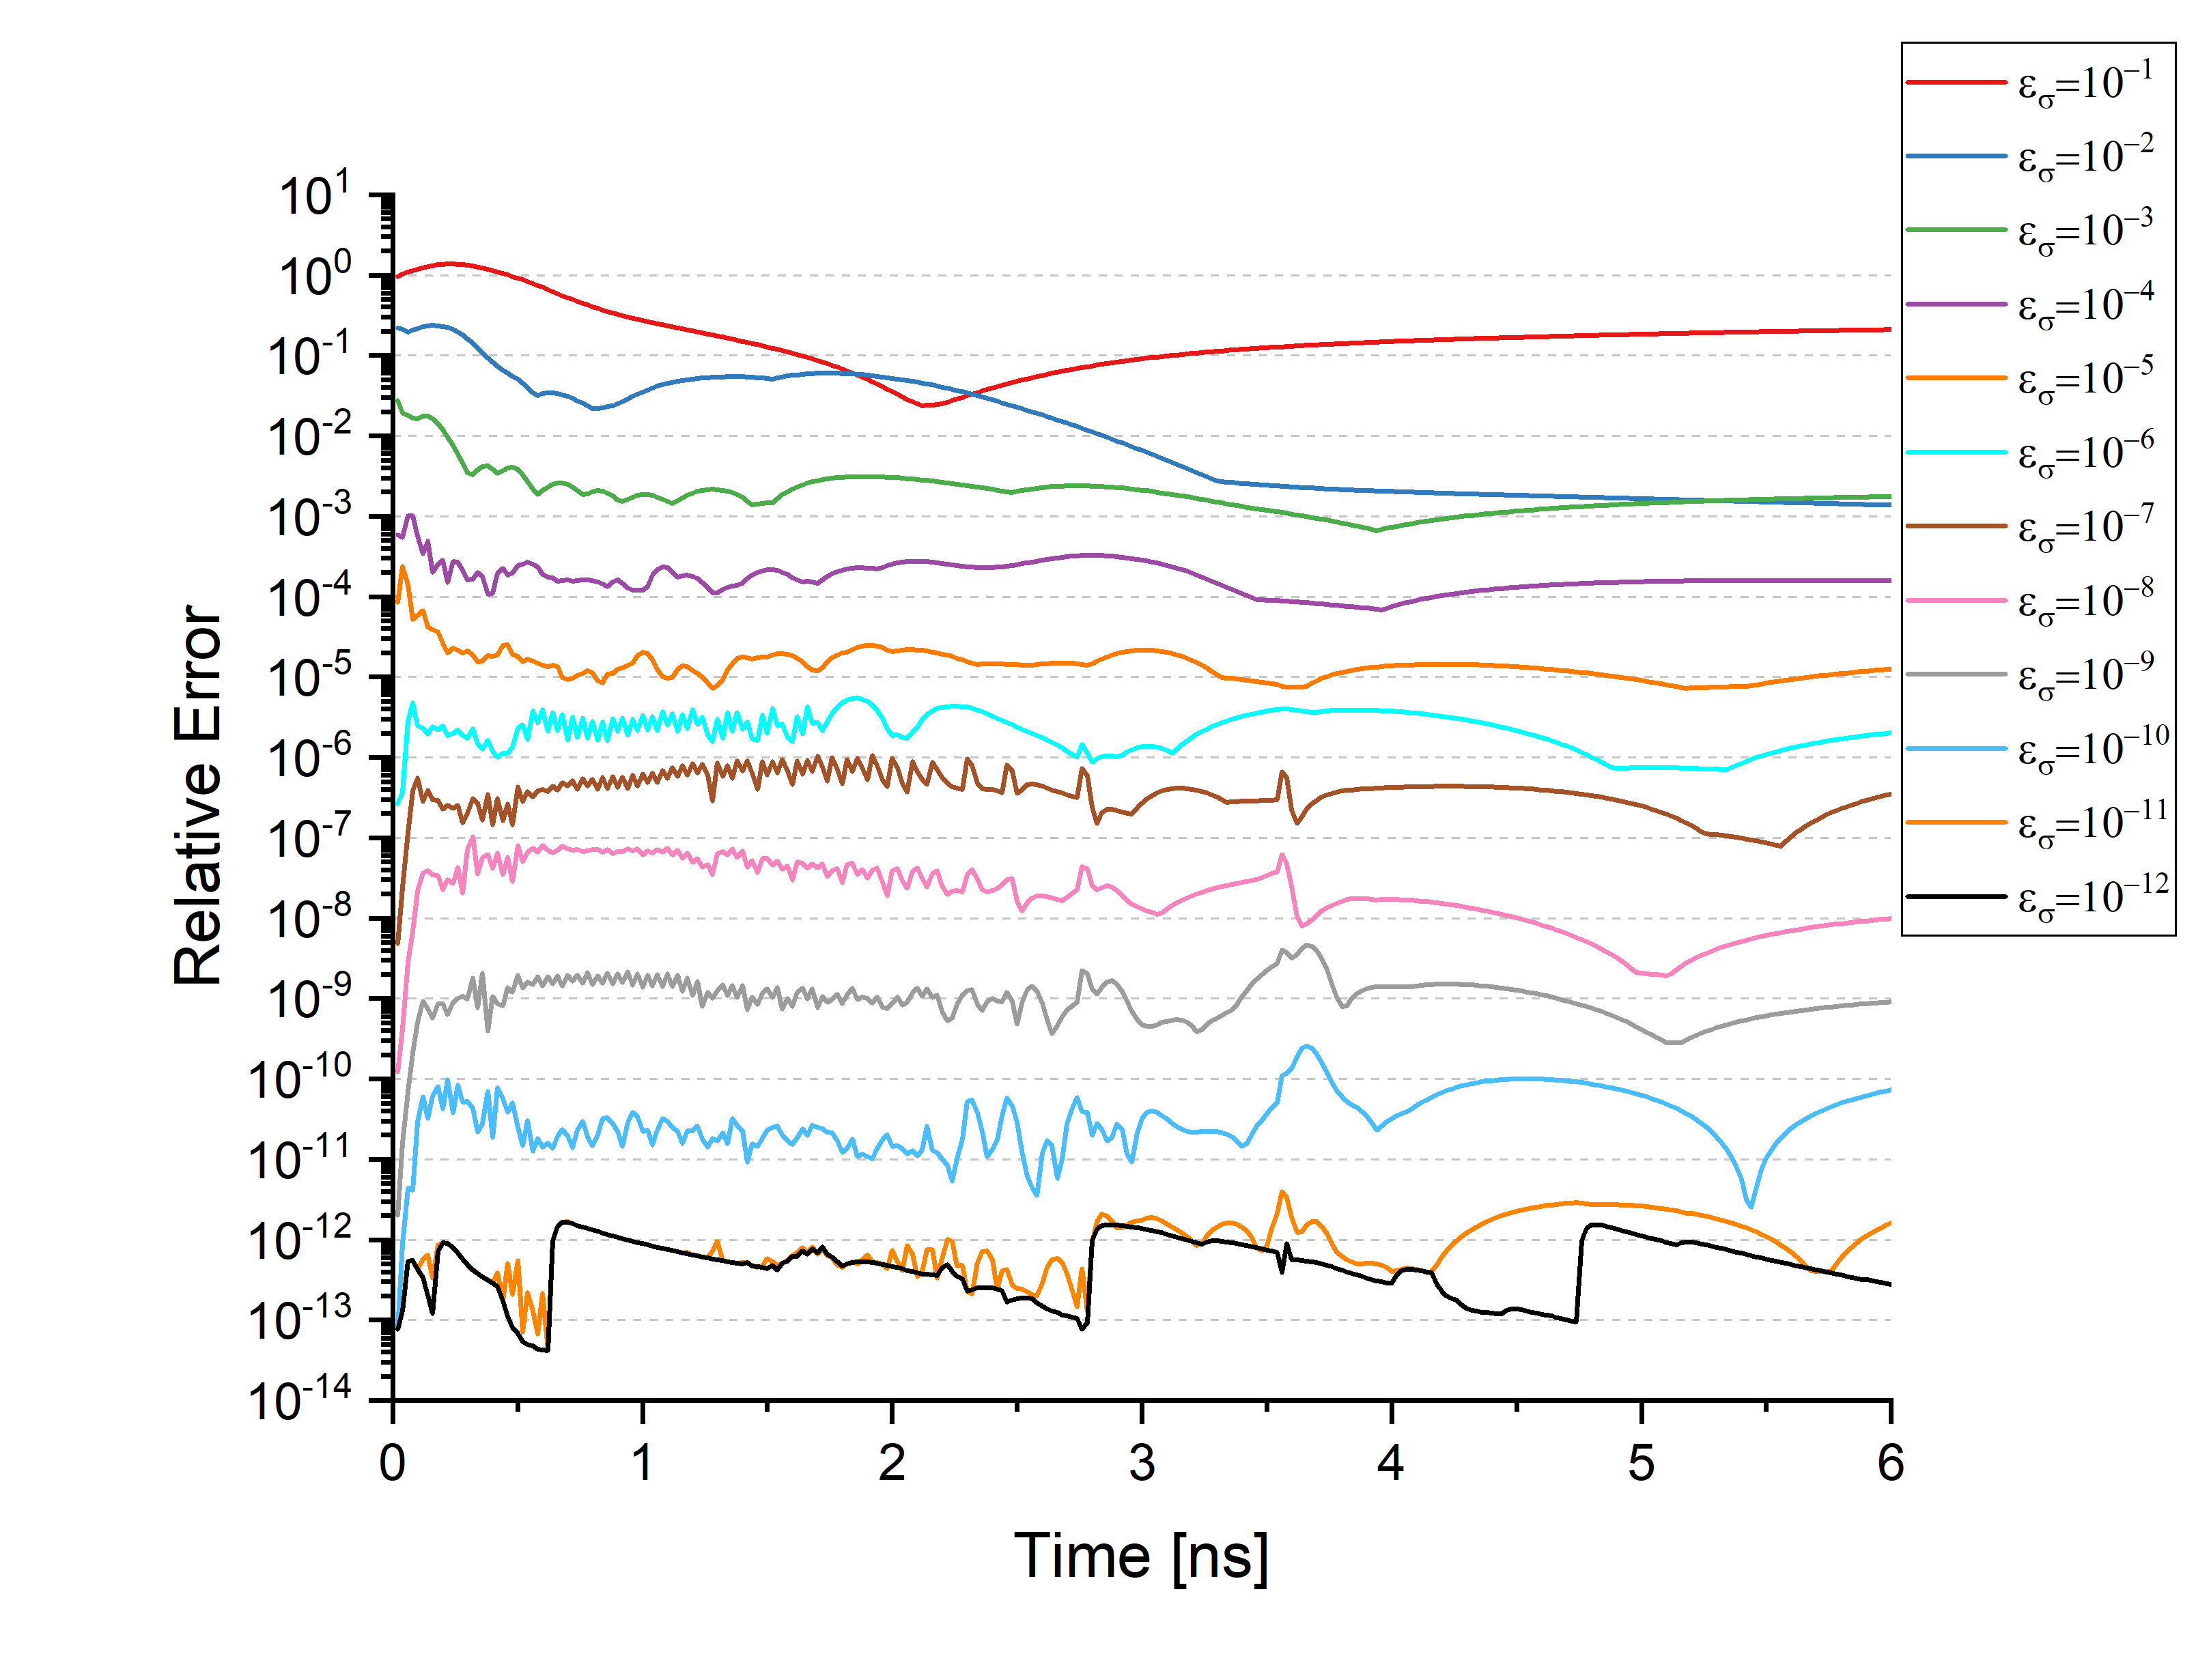
\includegraphics[width=0.475\textwidth]{refcase_E_rel_inf_fg_grey_bg.png}}\\
		\subfloat[reduced rank energy density temperature error \label{subfig:refcase_Temp_rel_inf_Eg_grey}]{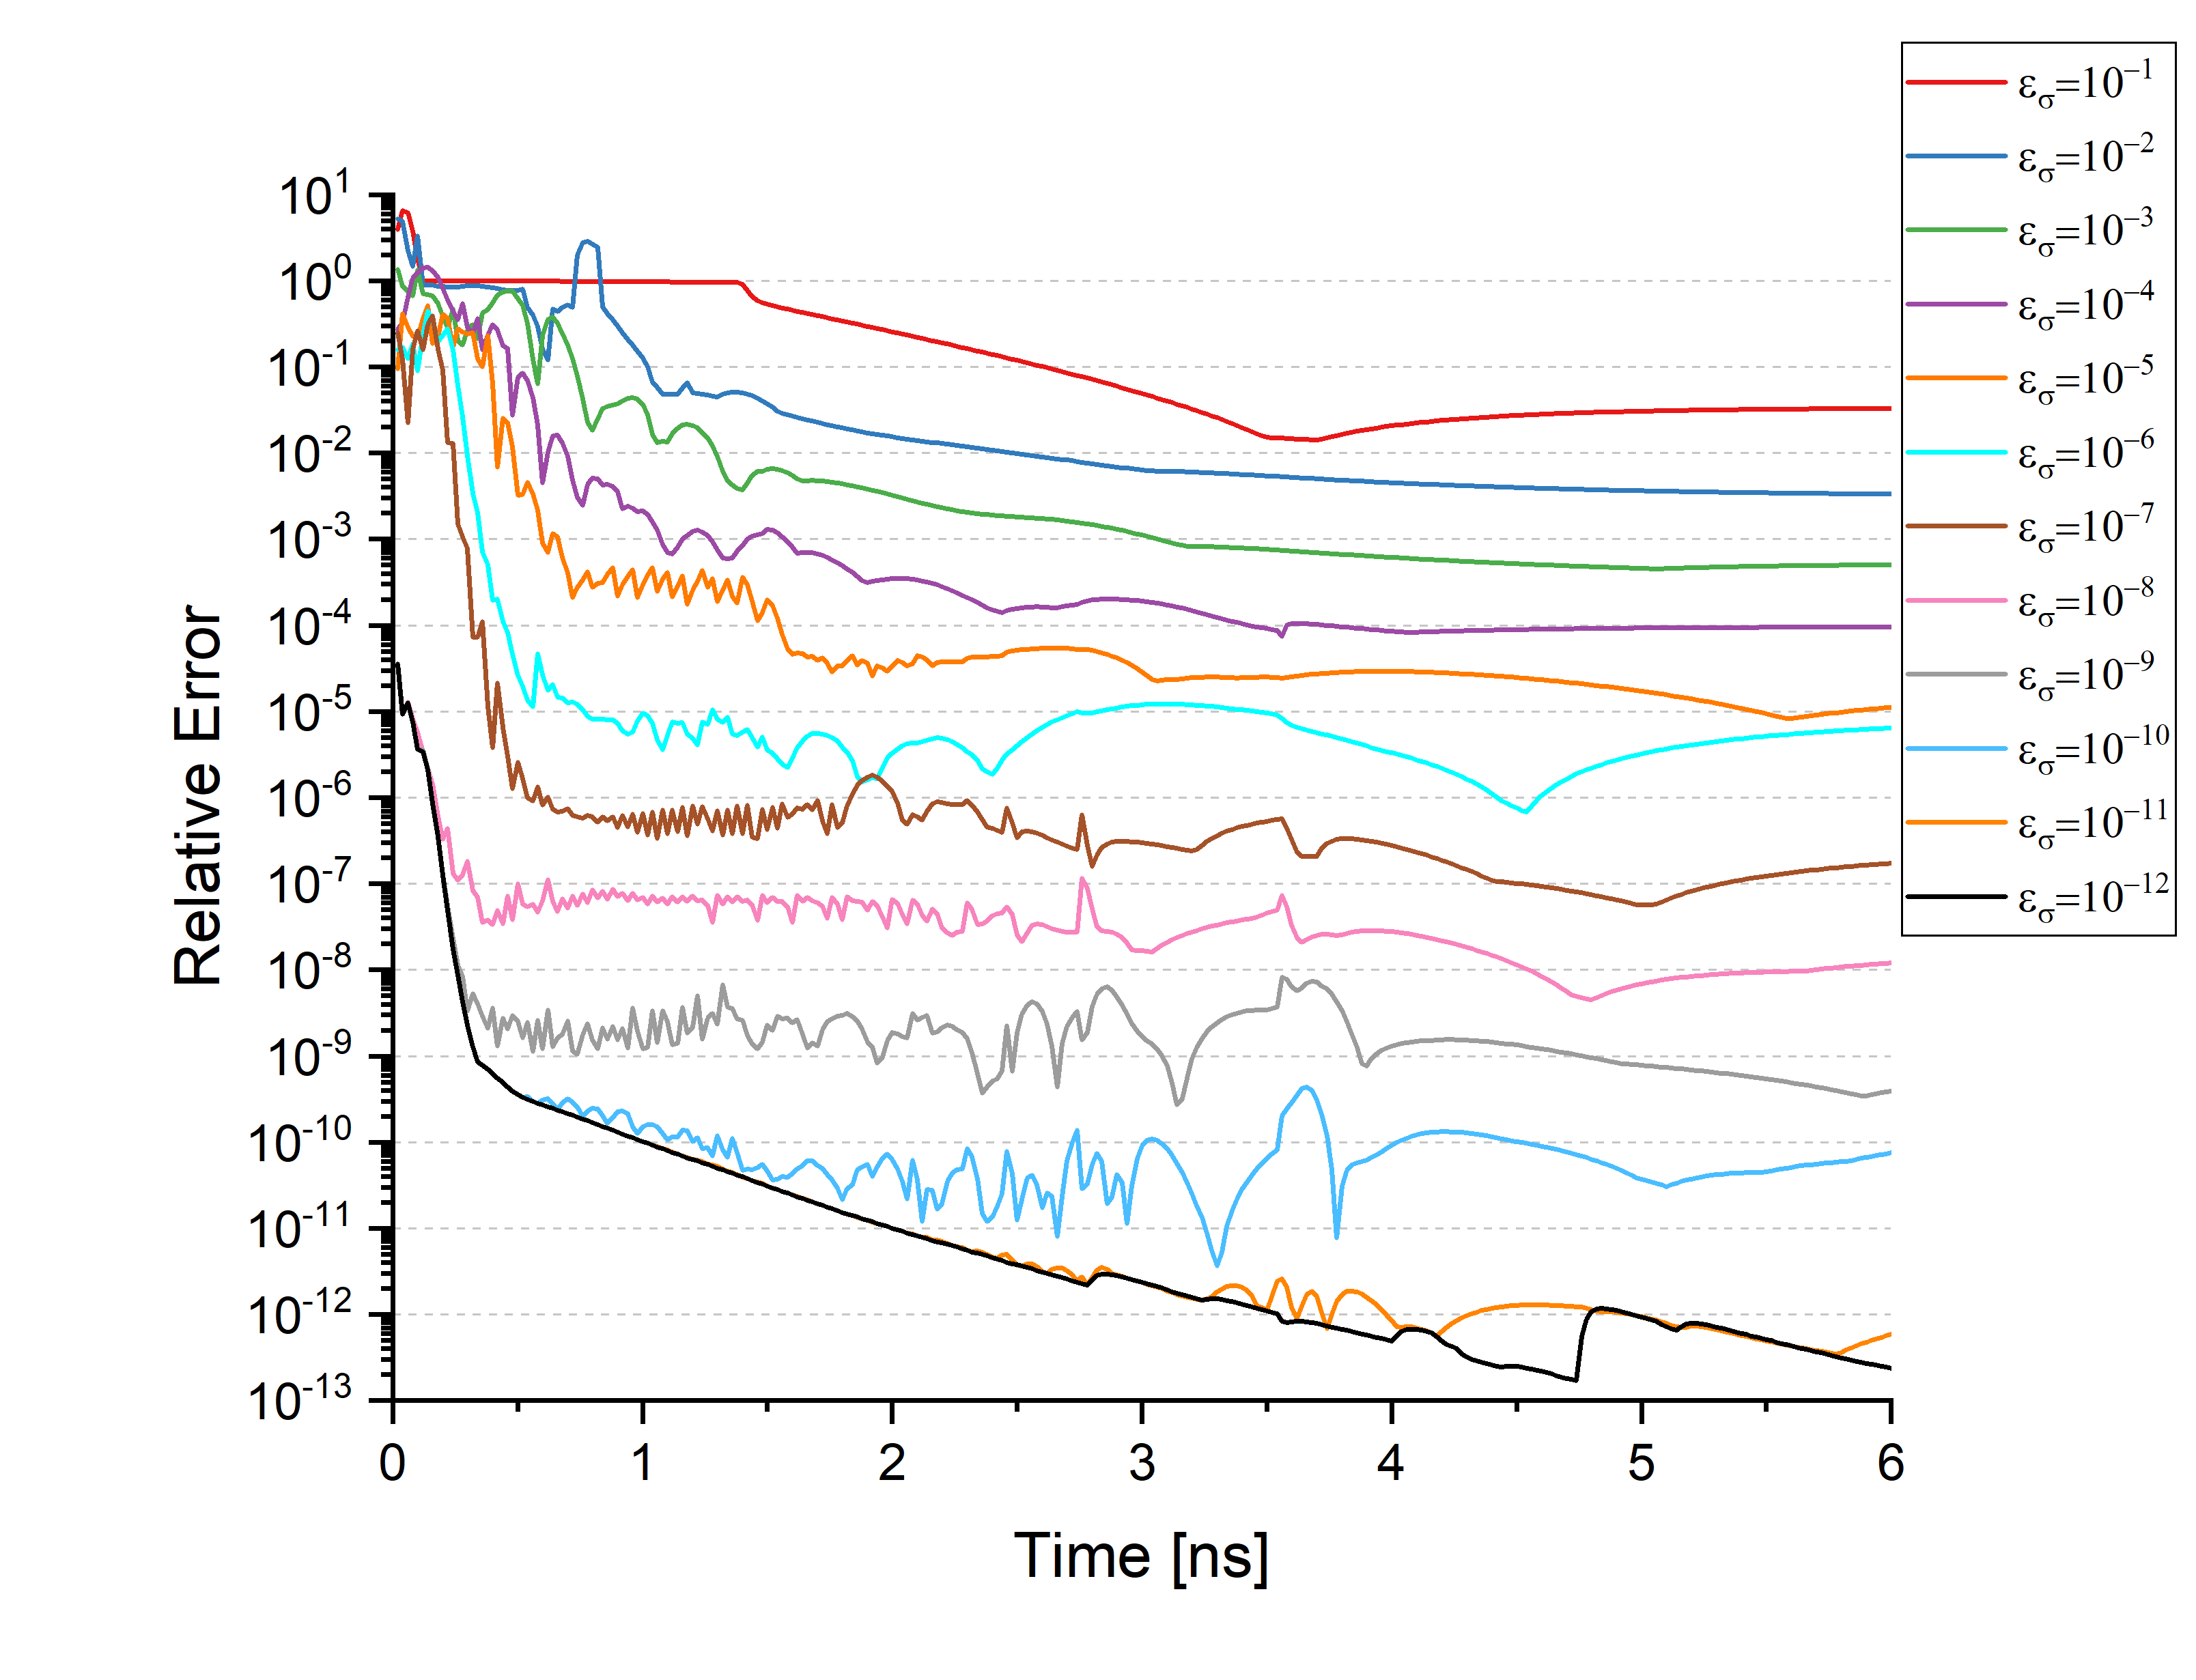
\includegraphics[width=0.475\textwidth]{refcase_Temp_rel_inf_Eg_grey_bg.png}}
		\subfloat[reduced rank energy density total energy density error \label{subfig:refcase_E_rel_inf_Eg_grey}]{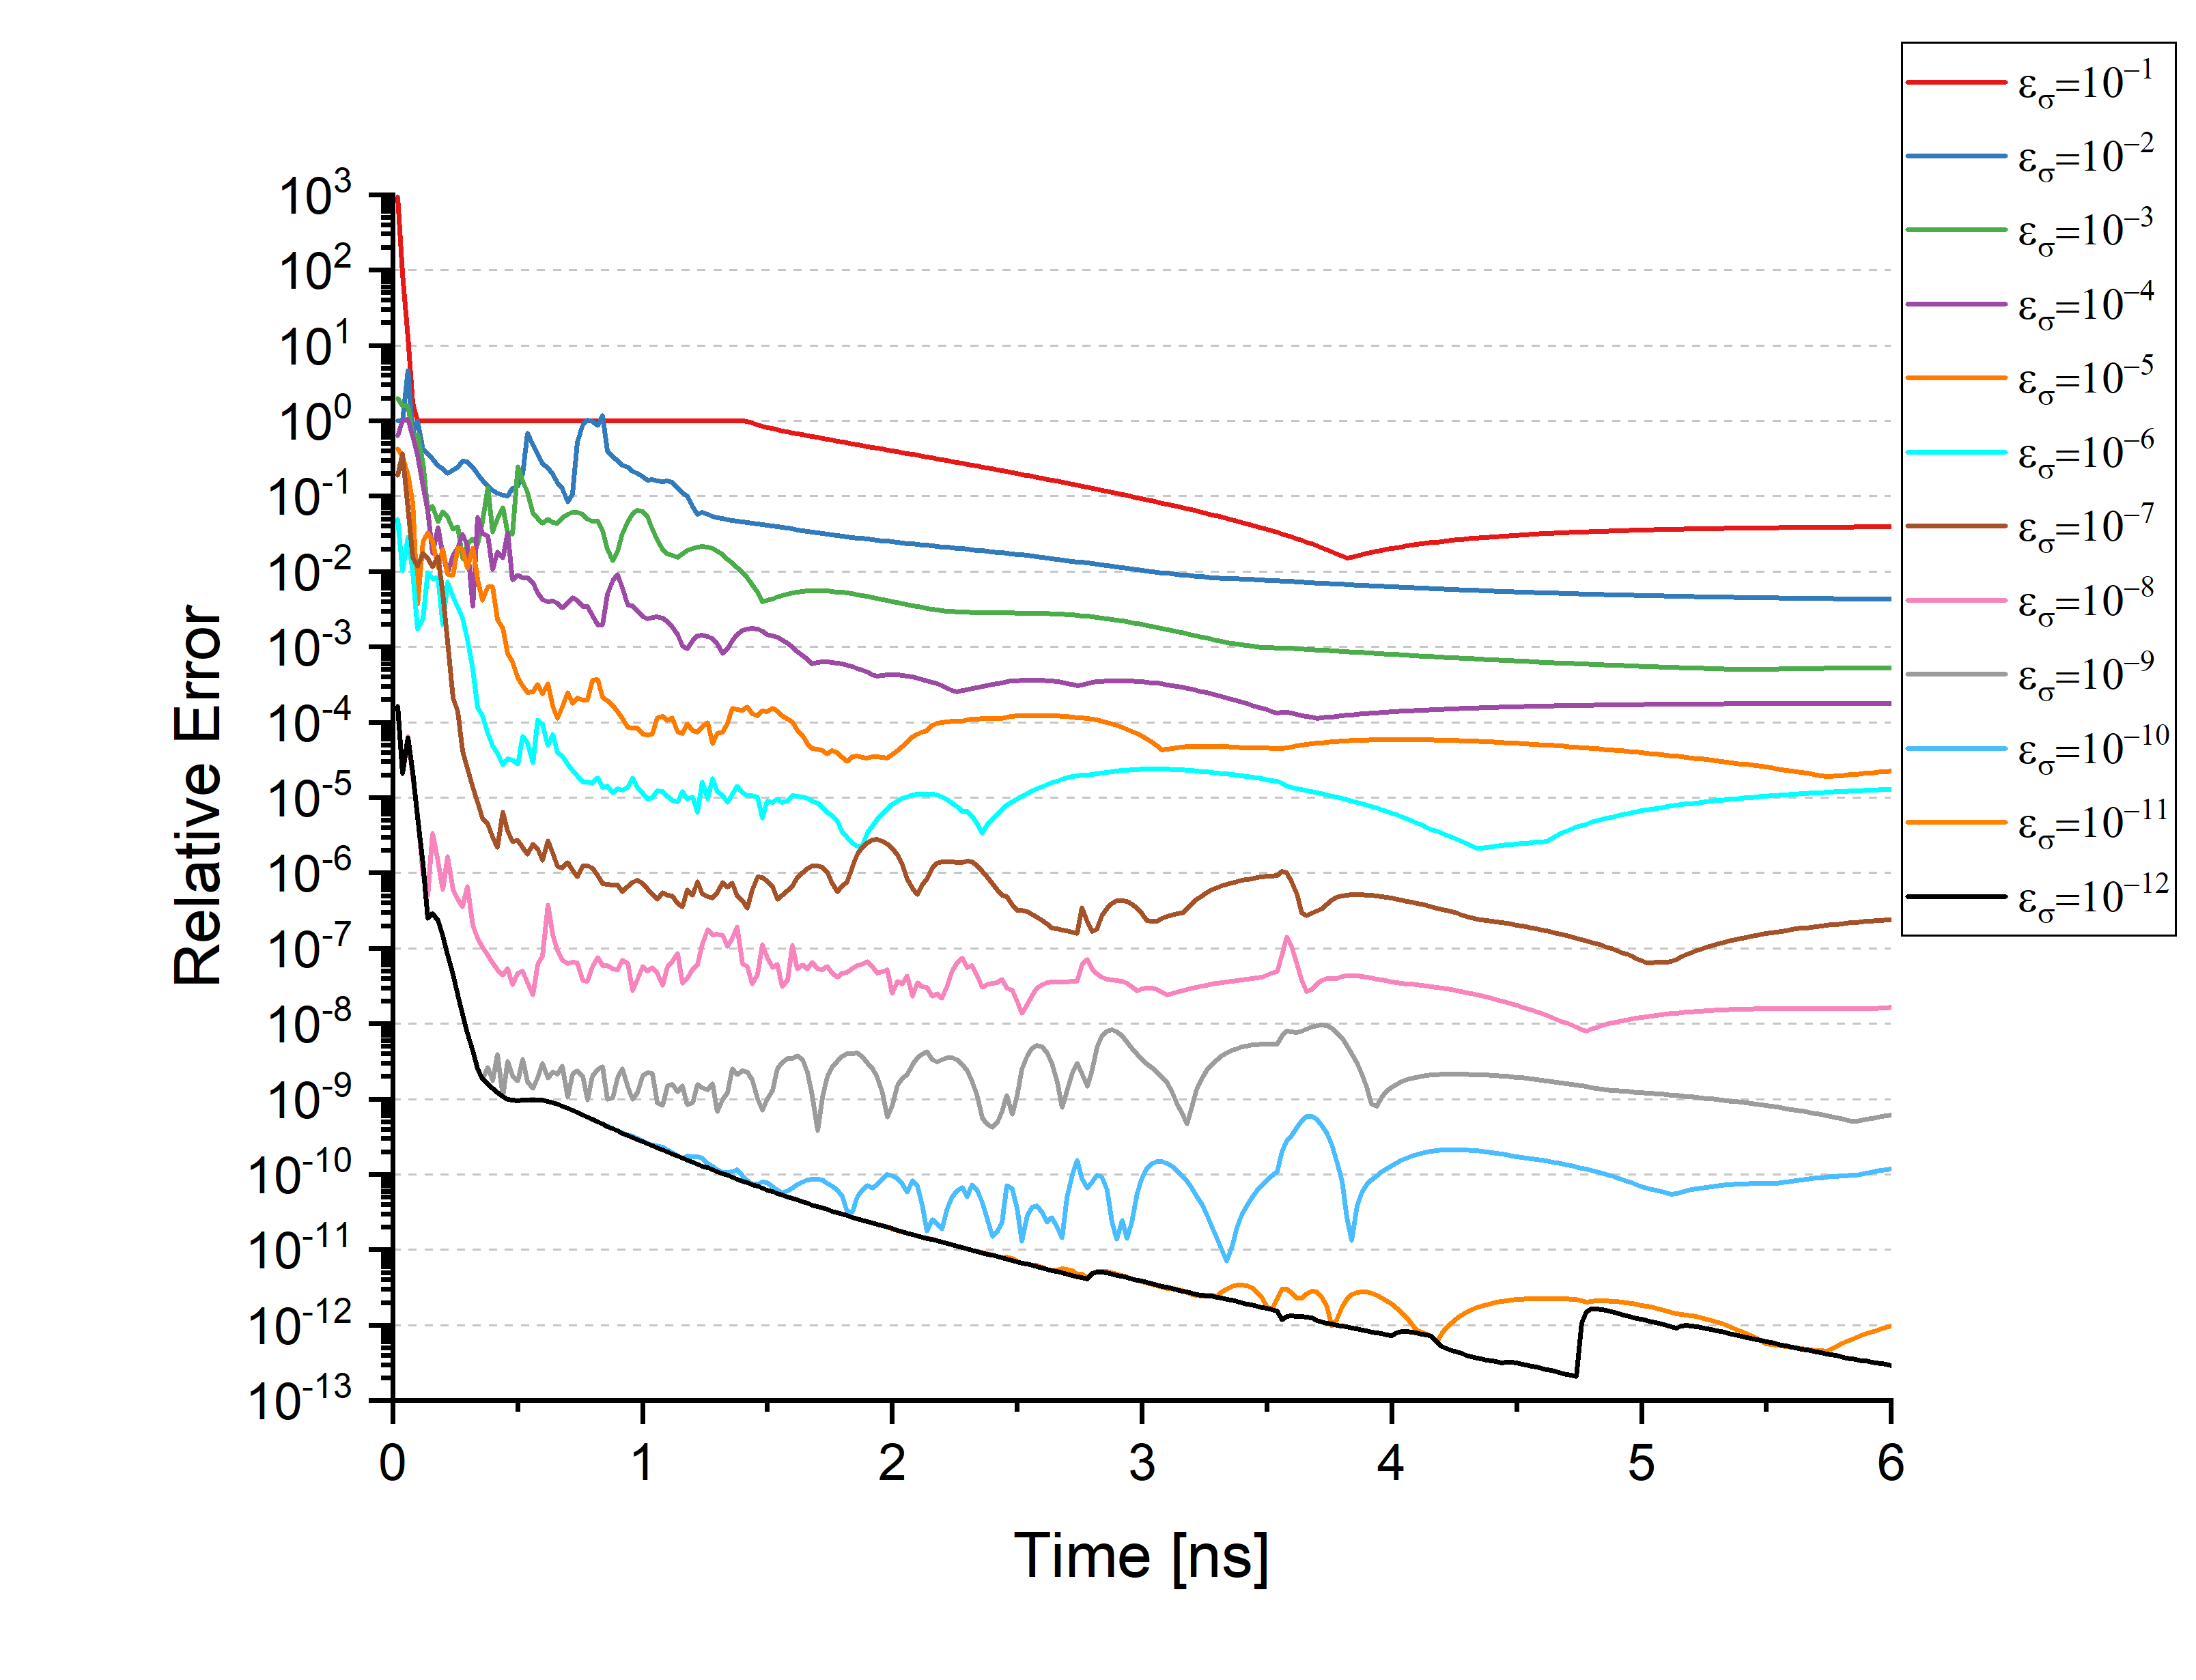
\includegraphics[width=0.475\textwidth]{refcase_E_rel_inf_Eg_grey_bg.png}}\\
		\subfloat[reduced rank QD factor \& energy density \newline temperature error \label{subfig:refcase_Temp_rel_inf_E-fg_grey}]{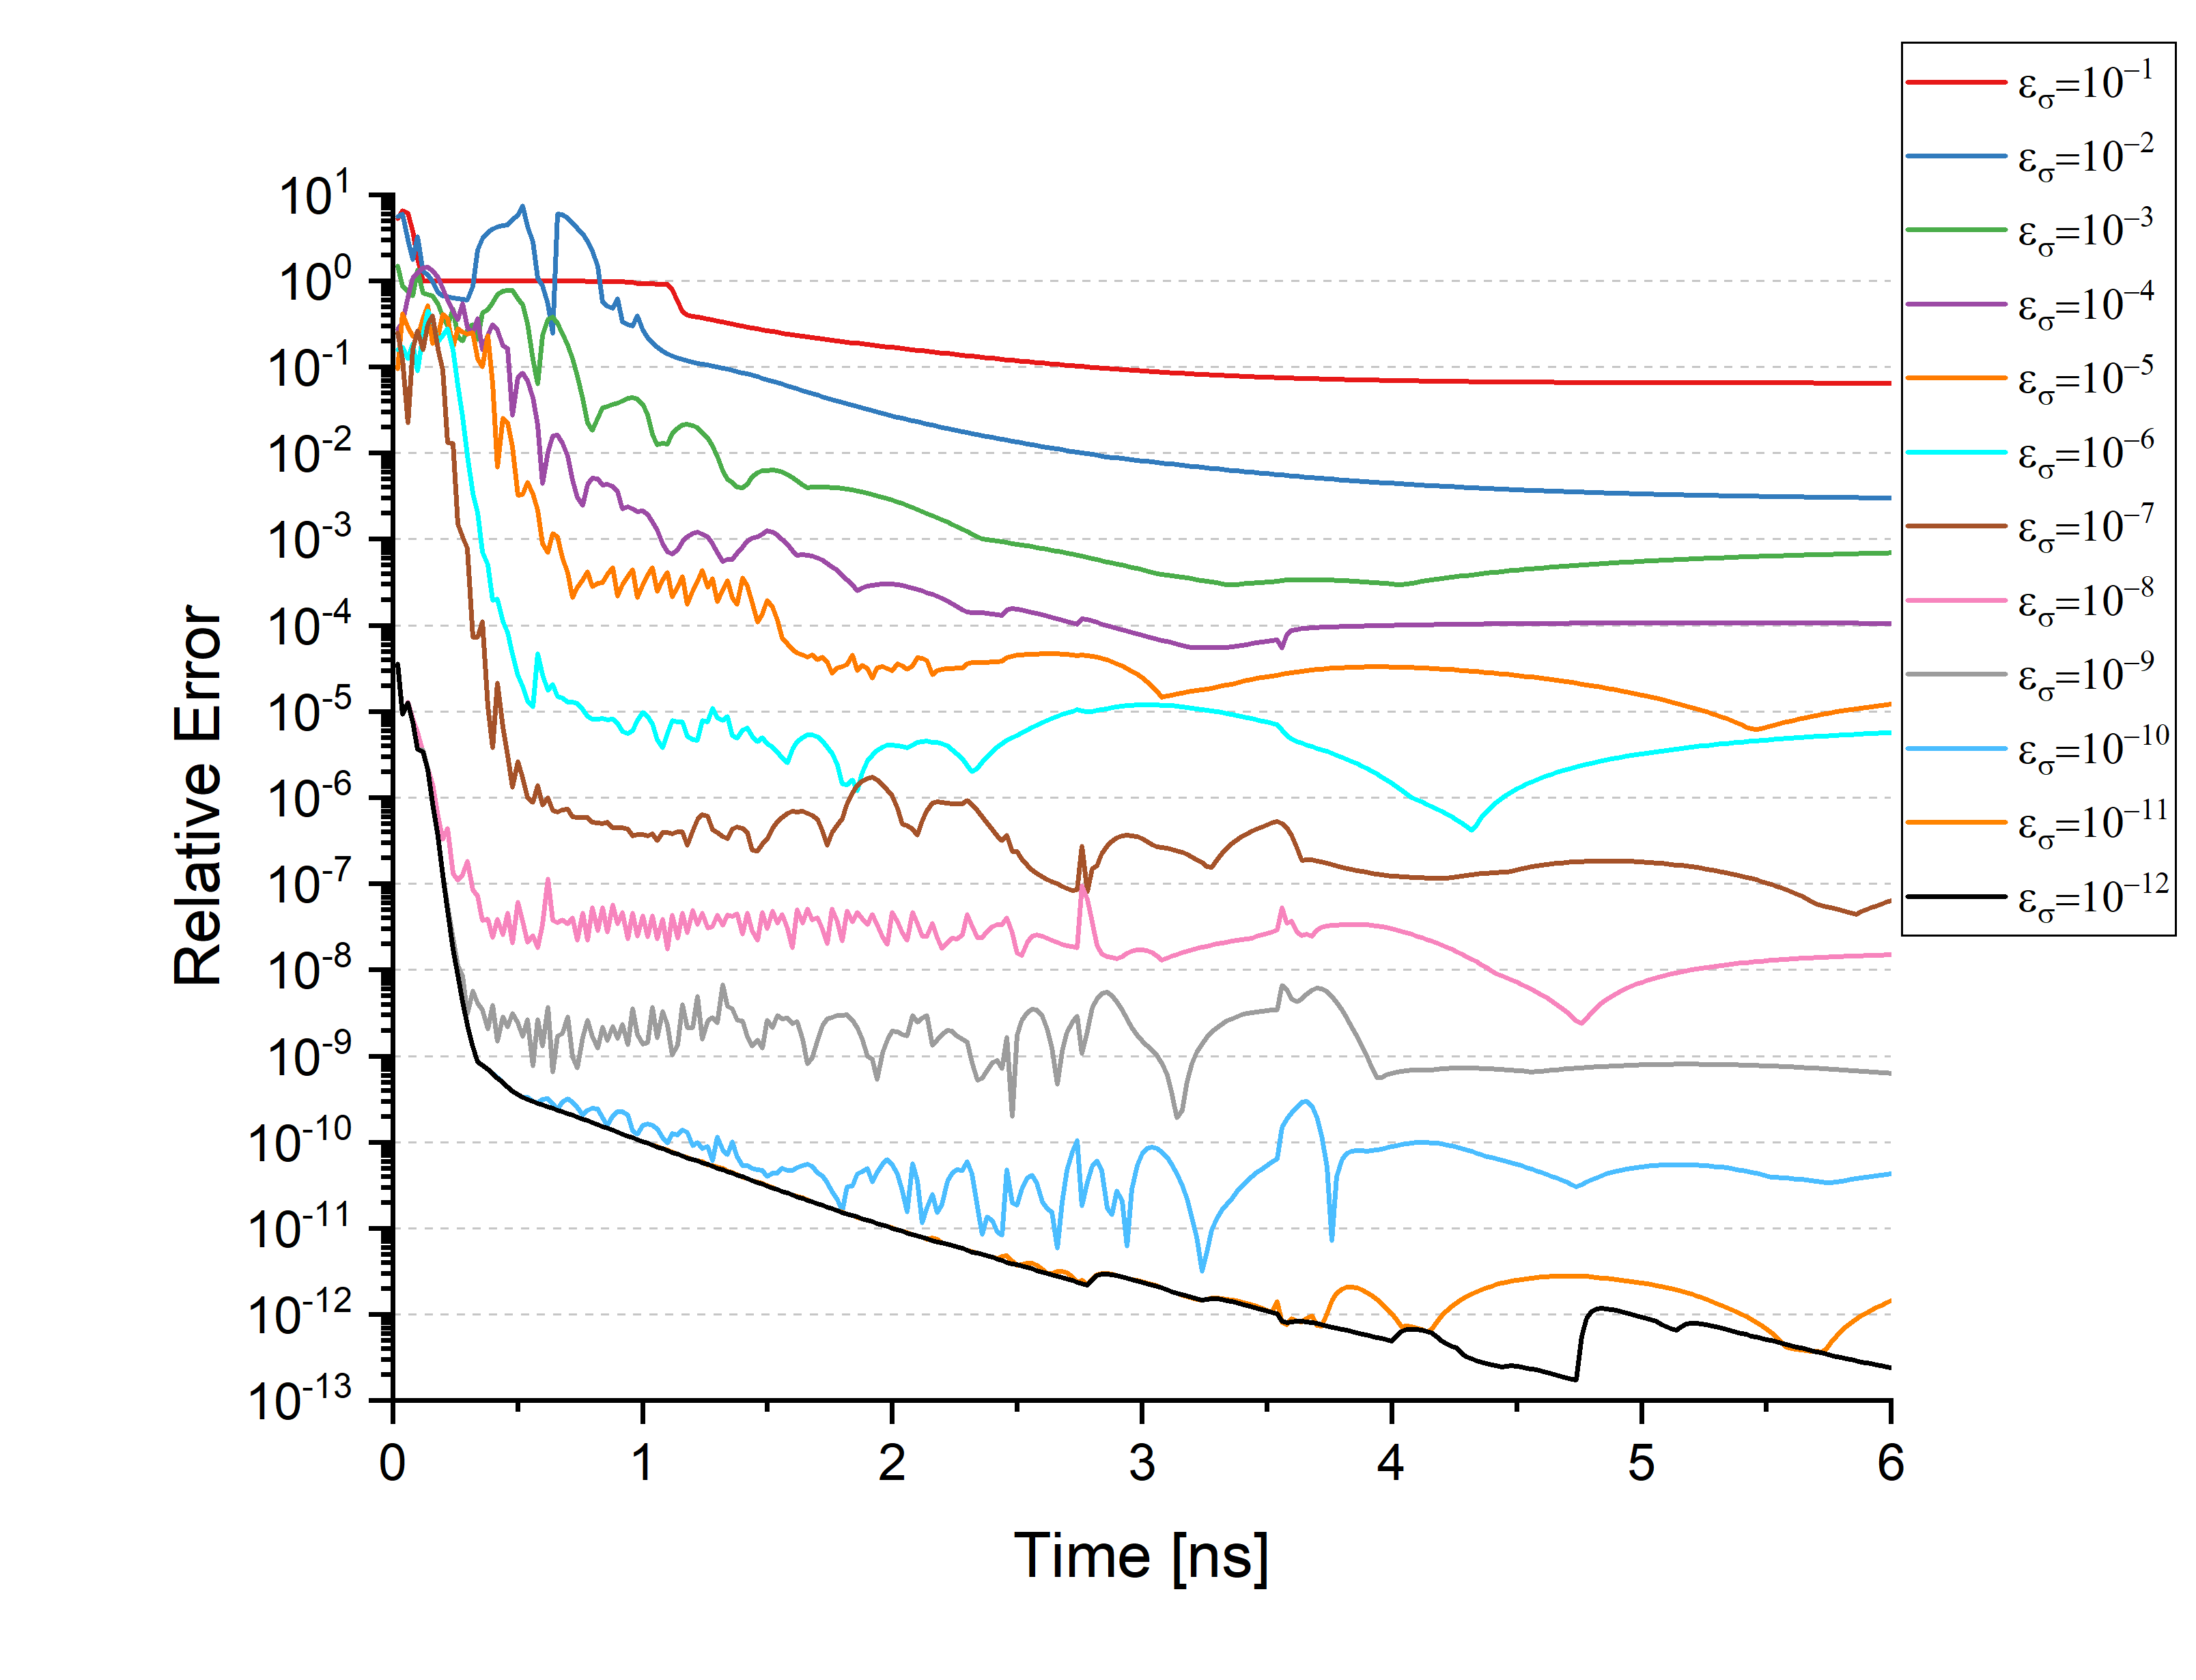
\includegraphics[width=0.475\textwidth]{refcase_Temp_rel_inf_E-fg_grey_bg.png}}
		\subfloat[reduced rank QD factor \& energy density total energy density error \label{subfig:refcase_E_rel_inf_E-fg_grey}]{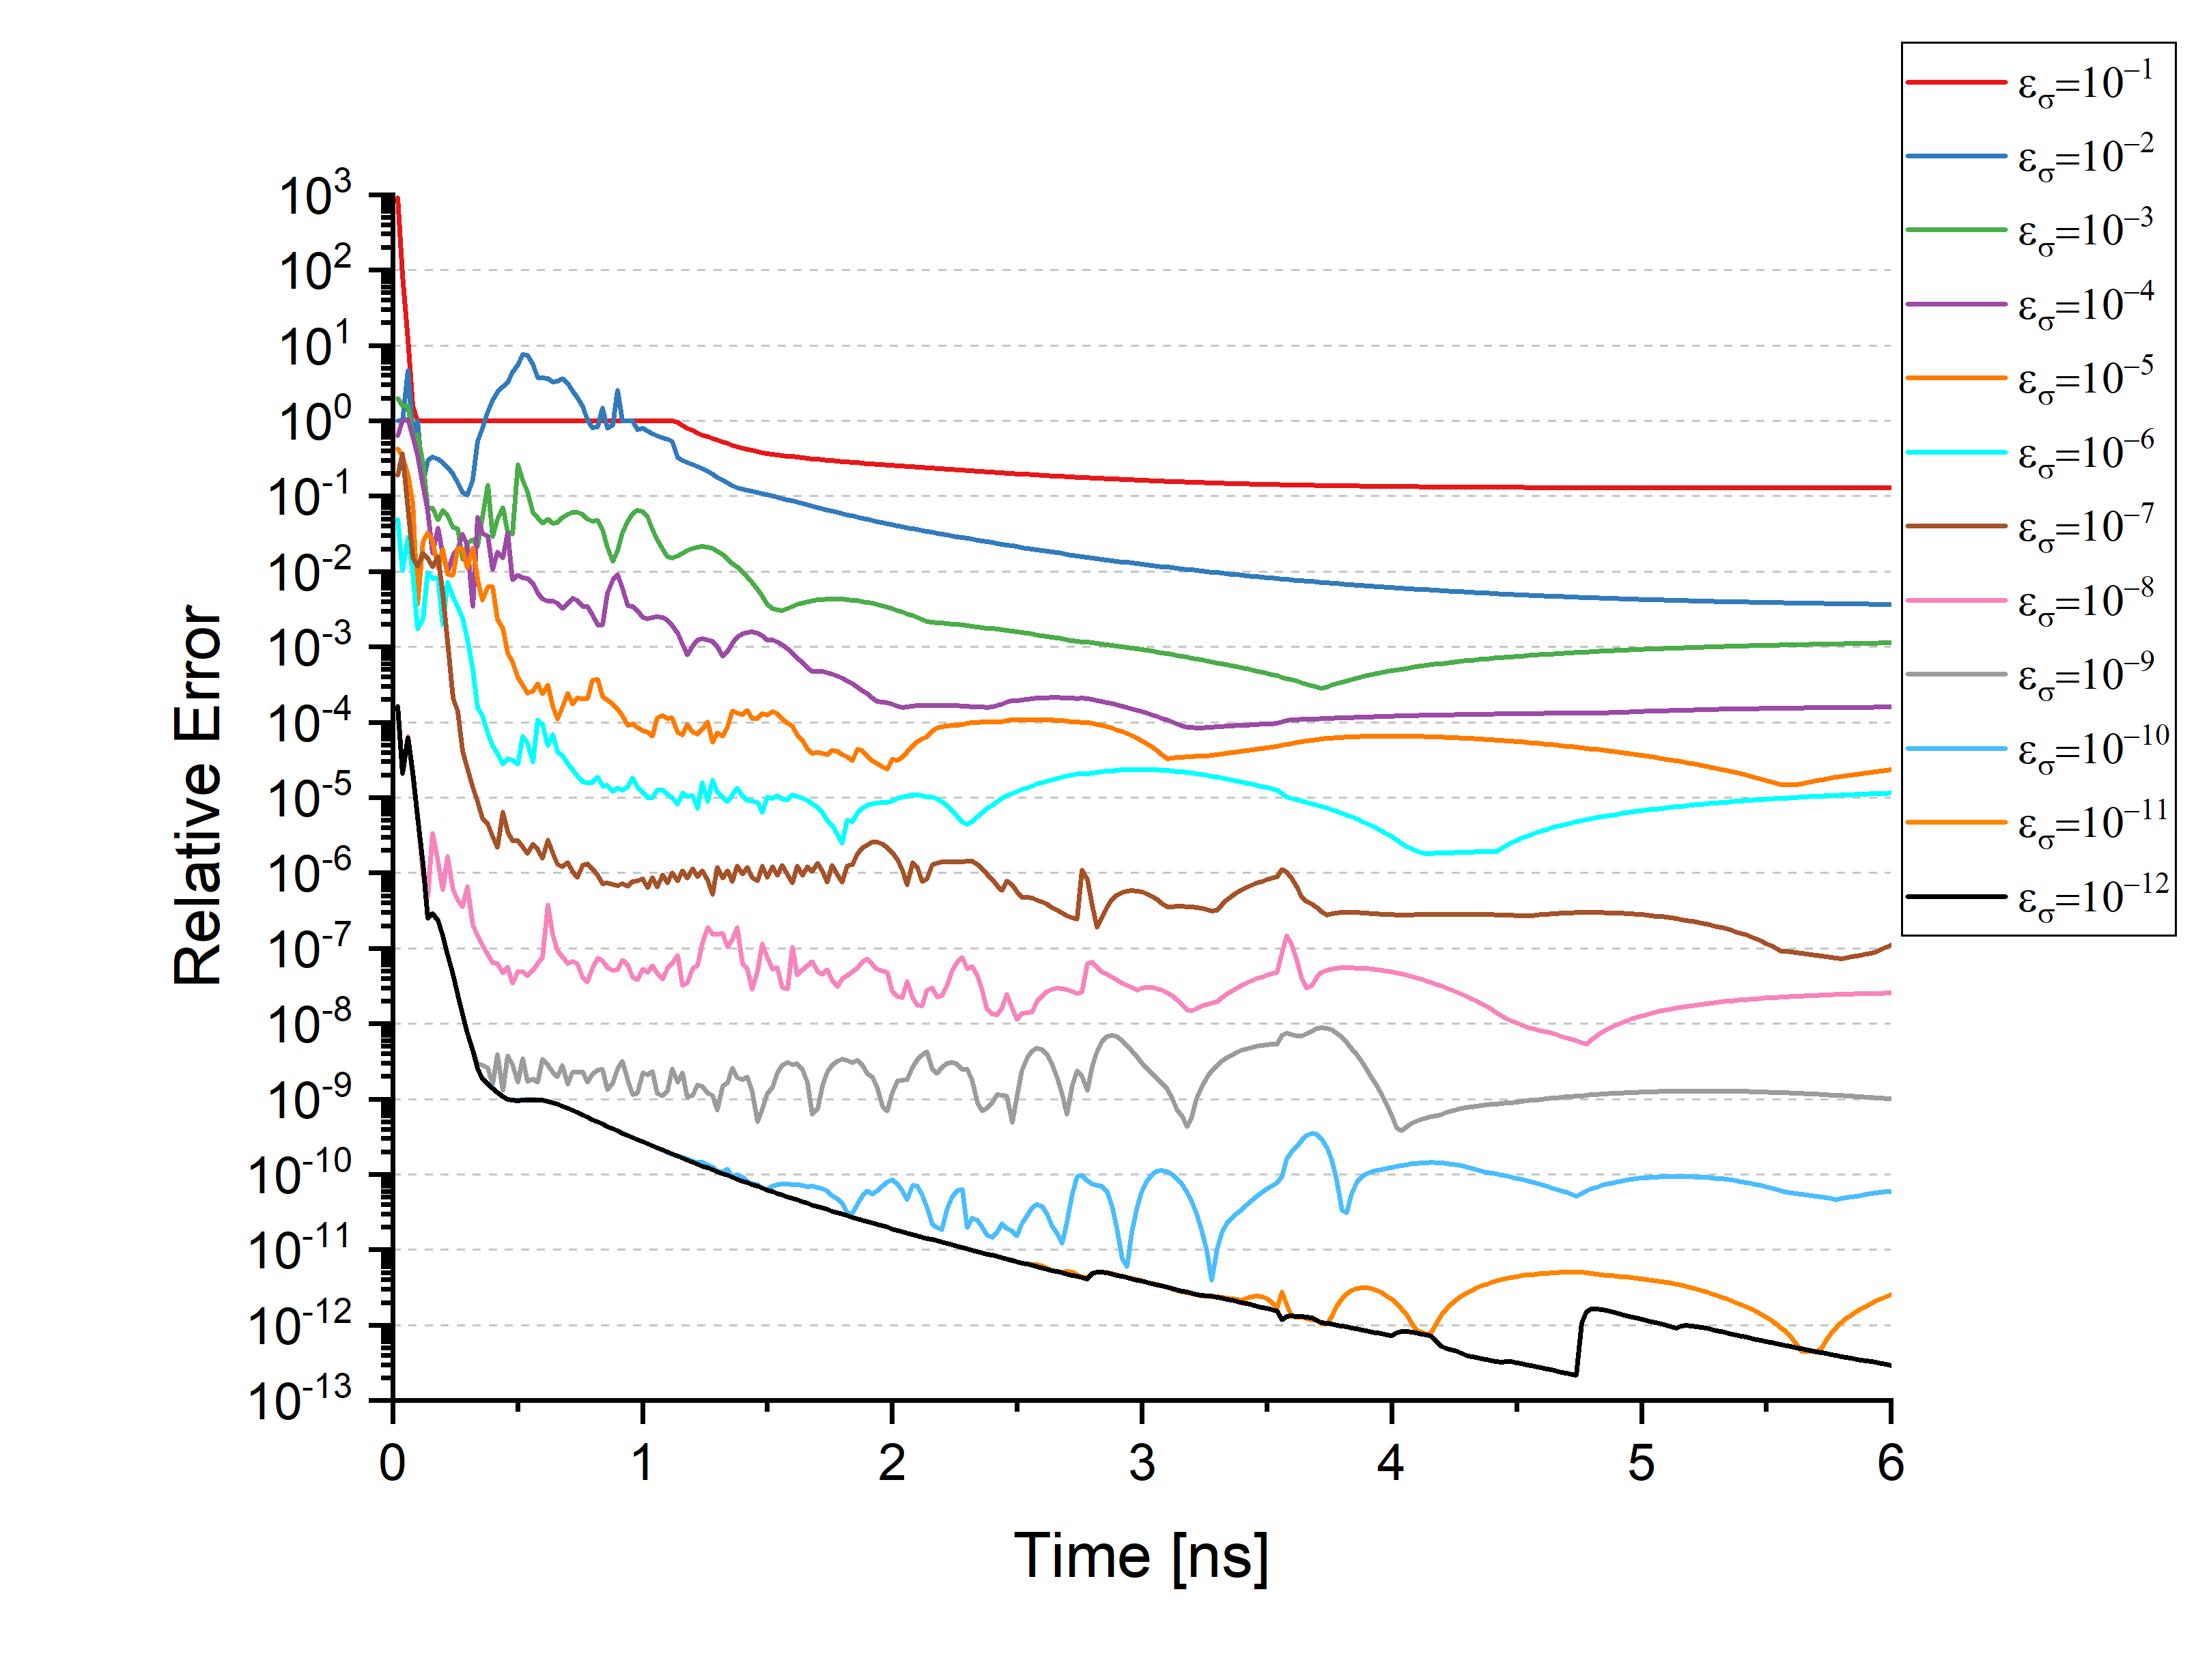
\includegraphics[width=0.475\textwidth]{refcase_E_rel_inf_E-fg_grey_bg.png}}\\
		\caption{\label{fig:ref_errs_inf_grey}
			Error of the GLOQD-POD ROM solution to the F-C test problem with relative to the high order MLQD solution in $\infty$ norm for various $\varepsilon_\sigma$ values}
	\end{figure}

	\begin{figure}[ht!]
		\centering
		\subfloat[Temperature error \label{subfig:refcase_Temp_domain_err_Eg_grey}]{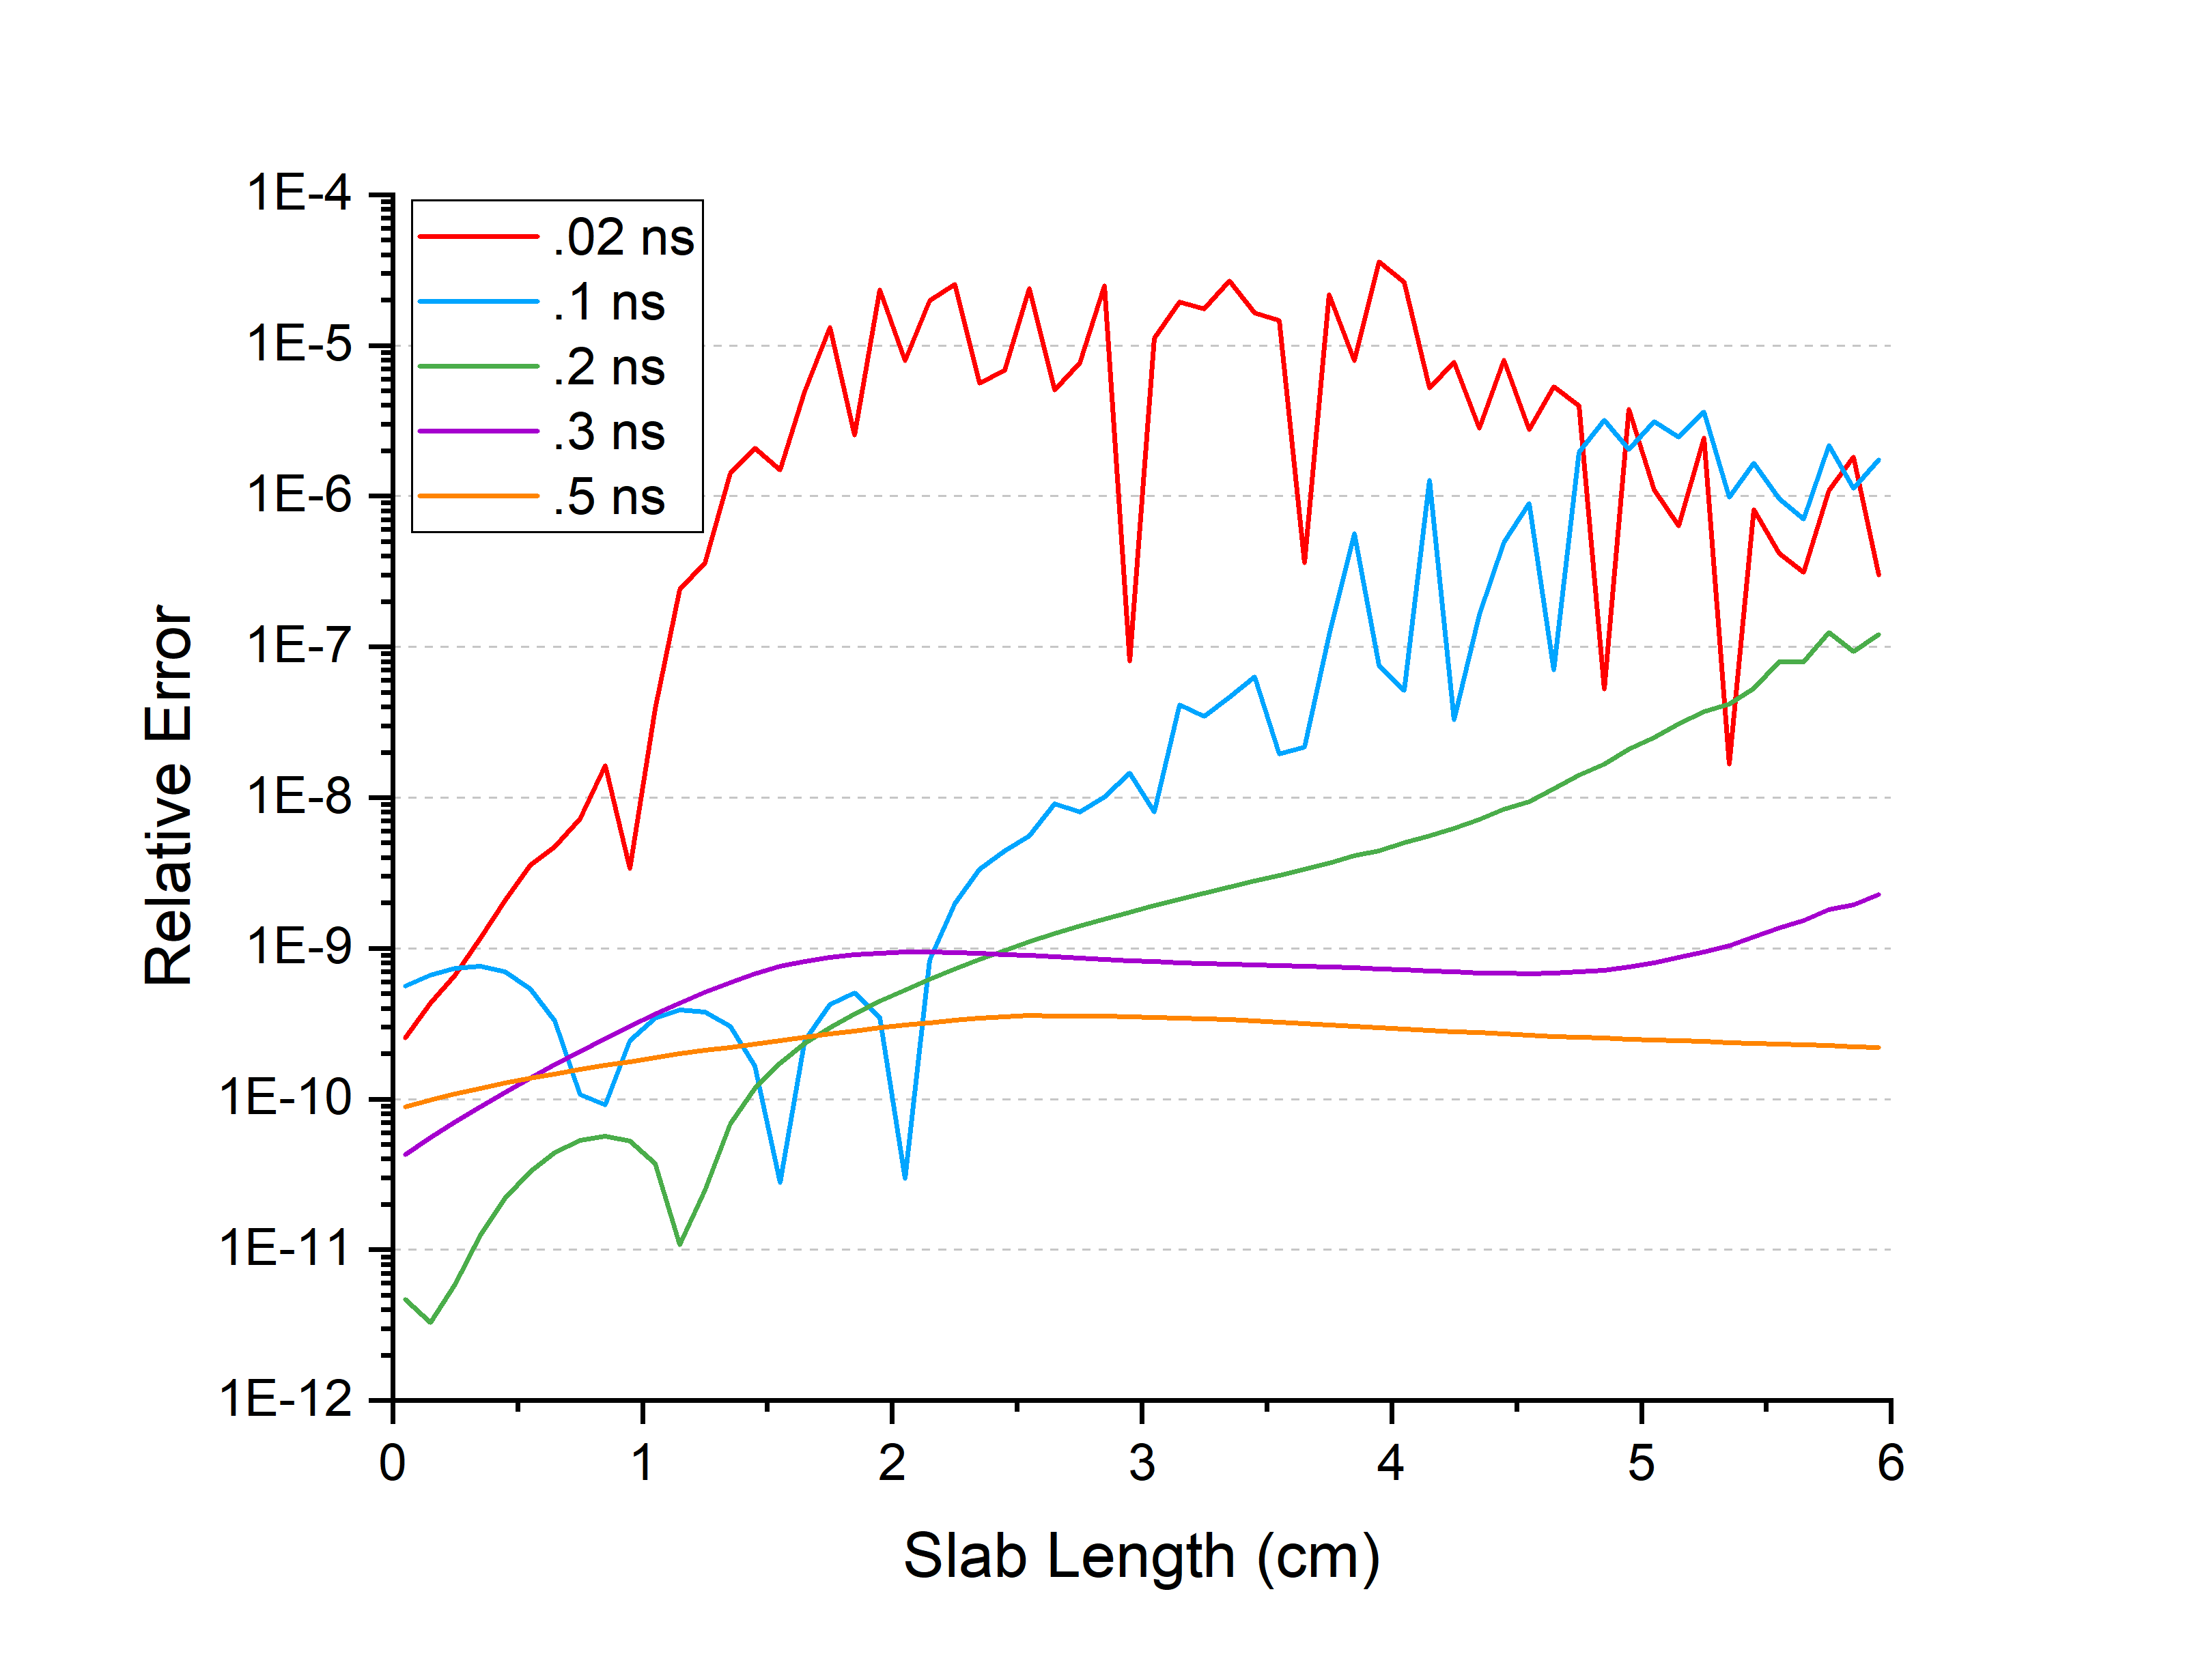
\includegraphics[width=0.5\textwidth]{refcase_Temp_domain_err_Eg_grey_bg.png}}
		\subfloat[Total energy density error \label{subfig:refcase_E_domain_err_Eg_grey}]{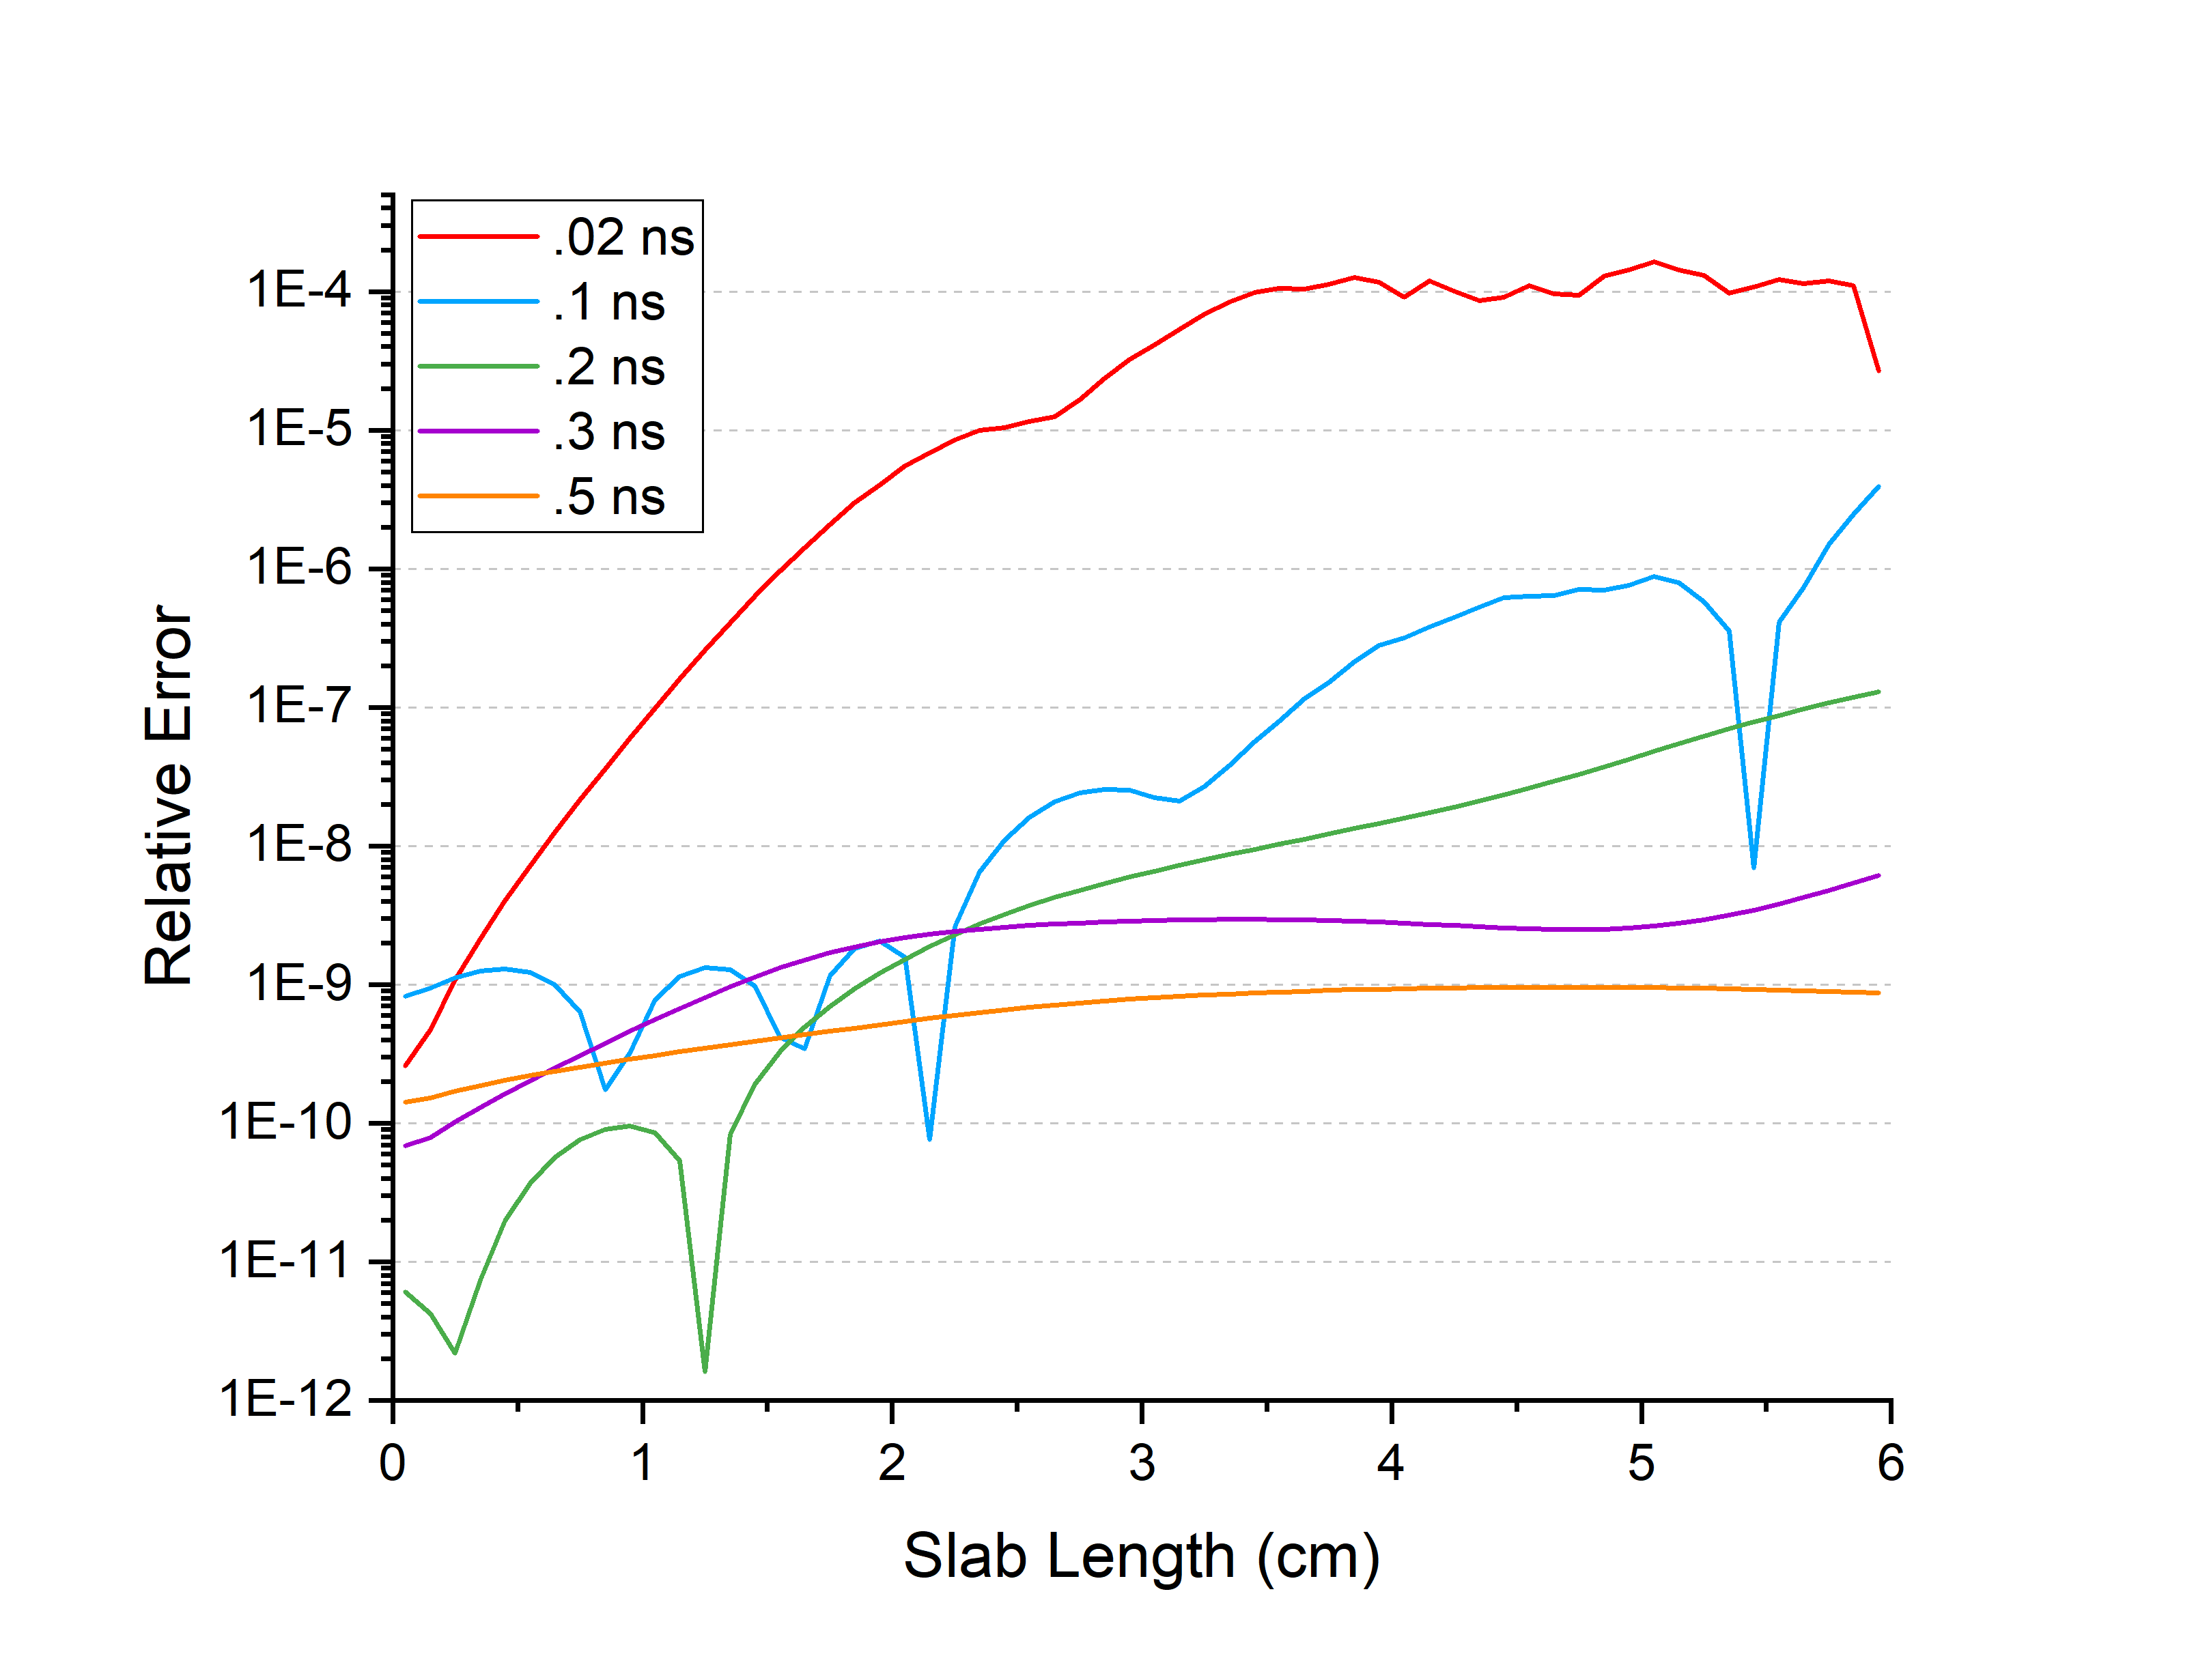
\includegraphics[width=0.5\textwidth]{refcase_E_domain_err_Eg_grey_bg.png}}
		\caption{\label{fig:ref_errs_domain_grey}
			Error of the MLQD-POD GLOQD solution to the F-C test problem relative to the high order solution for various time steps over the spatial domain with $\varepsilon_\sigma = 10^{-12}$}
	\end{figure}

	\ind The high errors demonstrated by the GLOQD-POD ROM for the early times of the problem show that more analysis must be done to try and improve the ROM before extending it further. Given the performance seen in Fig. \ref{fig:ref_errs_inf_grey}, the ROM is expected to produce overly high errors during the early times of the problem. Solving a problem with reduced time step length or parameterizing the ROM will add increased errors from the interpolation performed on the databases, thus any analysis on extended versions of the GLOQD-POD ROM will be limited until work can be done to improve the original version. Even so, it is still useful to observe how these extensions of the GLOQD-POD ROM behave. 
	
	\ind The GLOQD-POD ROM is now extended to solve problems with a time step length smaller than that used to calculate the POD database. This requires the GLOQD-POD ROM to solve the F-C test for more instants of time than the database provides information for $\bfg^*$ and $\eg^*$ for times not included in the database are calculated with linear interpolation between recorded database values. Fig. \ref{fig:errors_dt-0.01_grey} shows the  relative error in $L_1$-norm of the GLOQD-POD ROM solution computed with $\Delta t \! =  \! 1\! \times  \!  10^{-2}$ ns using various values of $\varepsilon_{\sigma}$. Fig. \ref{fig:errors_dt-0.005_grey}  presents the relative error in the solutions computed with $\Delta t \! = \! 5\! \times  \! 10^{-3}$ ns. The error for most cases saturated at $\varepsilon_\sigma = 10^{-5},10^{-6}$ and so smaller $\varepsilon_\sigma$ are not shown. All cases have the most error at the early times of the problem which decreases by several orders of magnitude as the problem progresses. The cases which used reduced rank approximation of QD factors and exact energy densities had very similar errors to the cases shown for the MLOQD-POD ROM. This is to be expected as it should emulate the MLOQD-POD method since exact group energy densities are used. The saturation level error does not change significantly between cases that use the exact reference value and reduced rank forms of the group QD factors and energy densities. Note in Fig. \ref{fig:errors_dt-0.005_grey}, the error does not monotonically decrease as $\varepsilon_\sigma$ decreases. This effect is only present when using the reduced rank form of the group energy densities.
	
	%=================================================================================
	% REDUCED TIME STEP ERRORS PLOT
	\begin{figure}[ht!]
		\centering
		\subfloat[Temperature relative error using approximate \newline $f_g$ and reference $E_g$  \label{subfig:GR_bc1000-t001_qdf1000-t002_Tavg_grey_fg}]{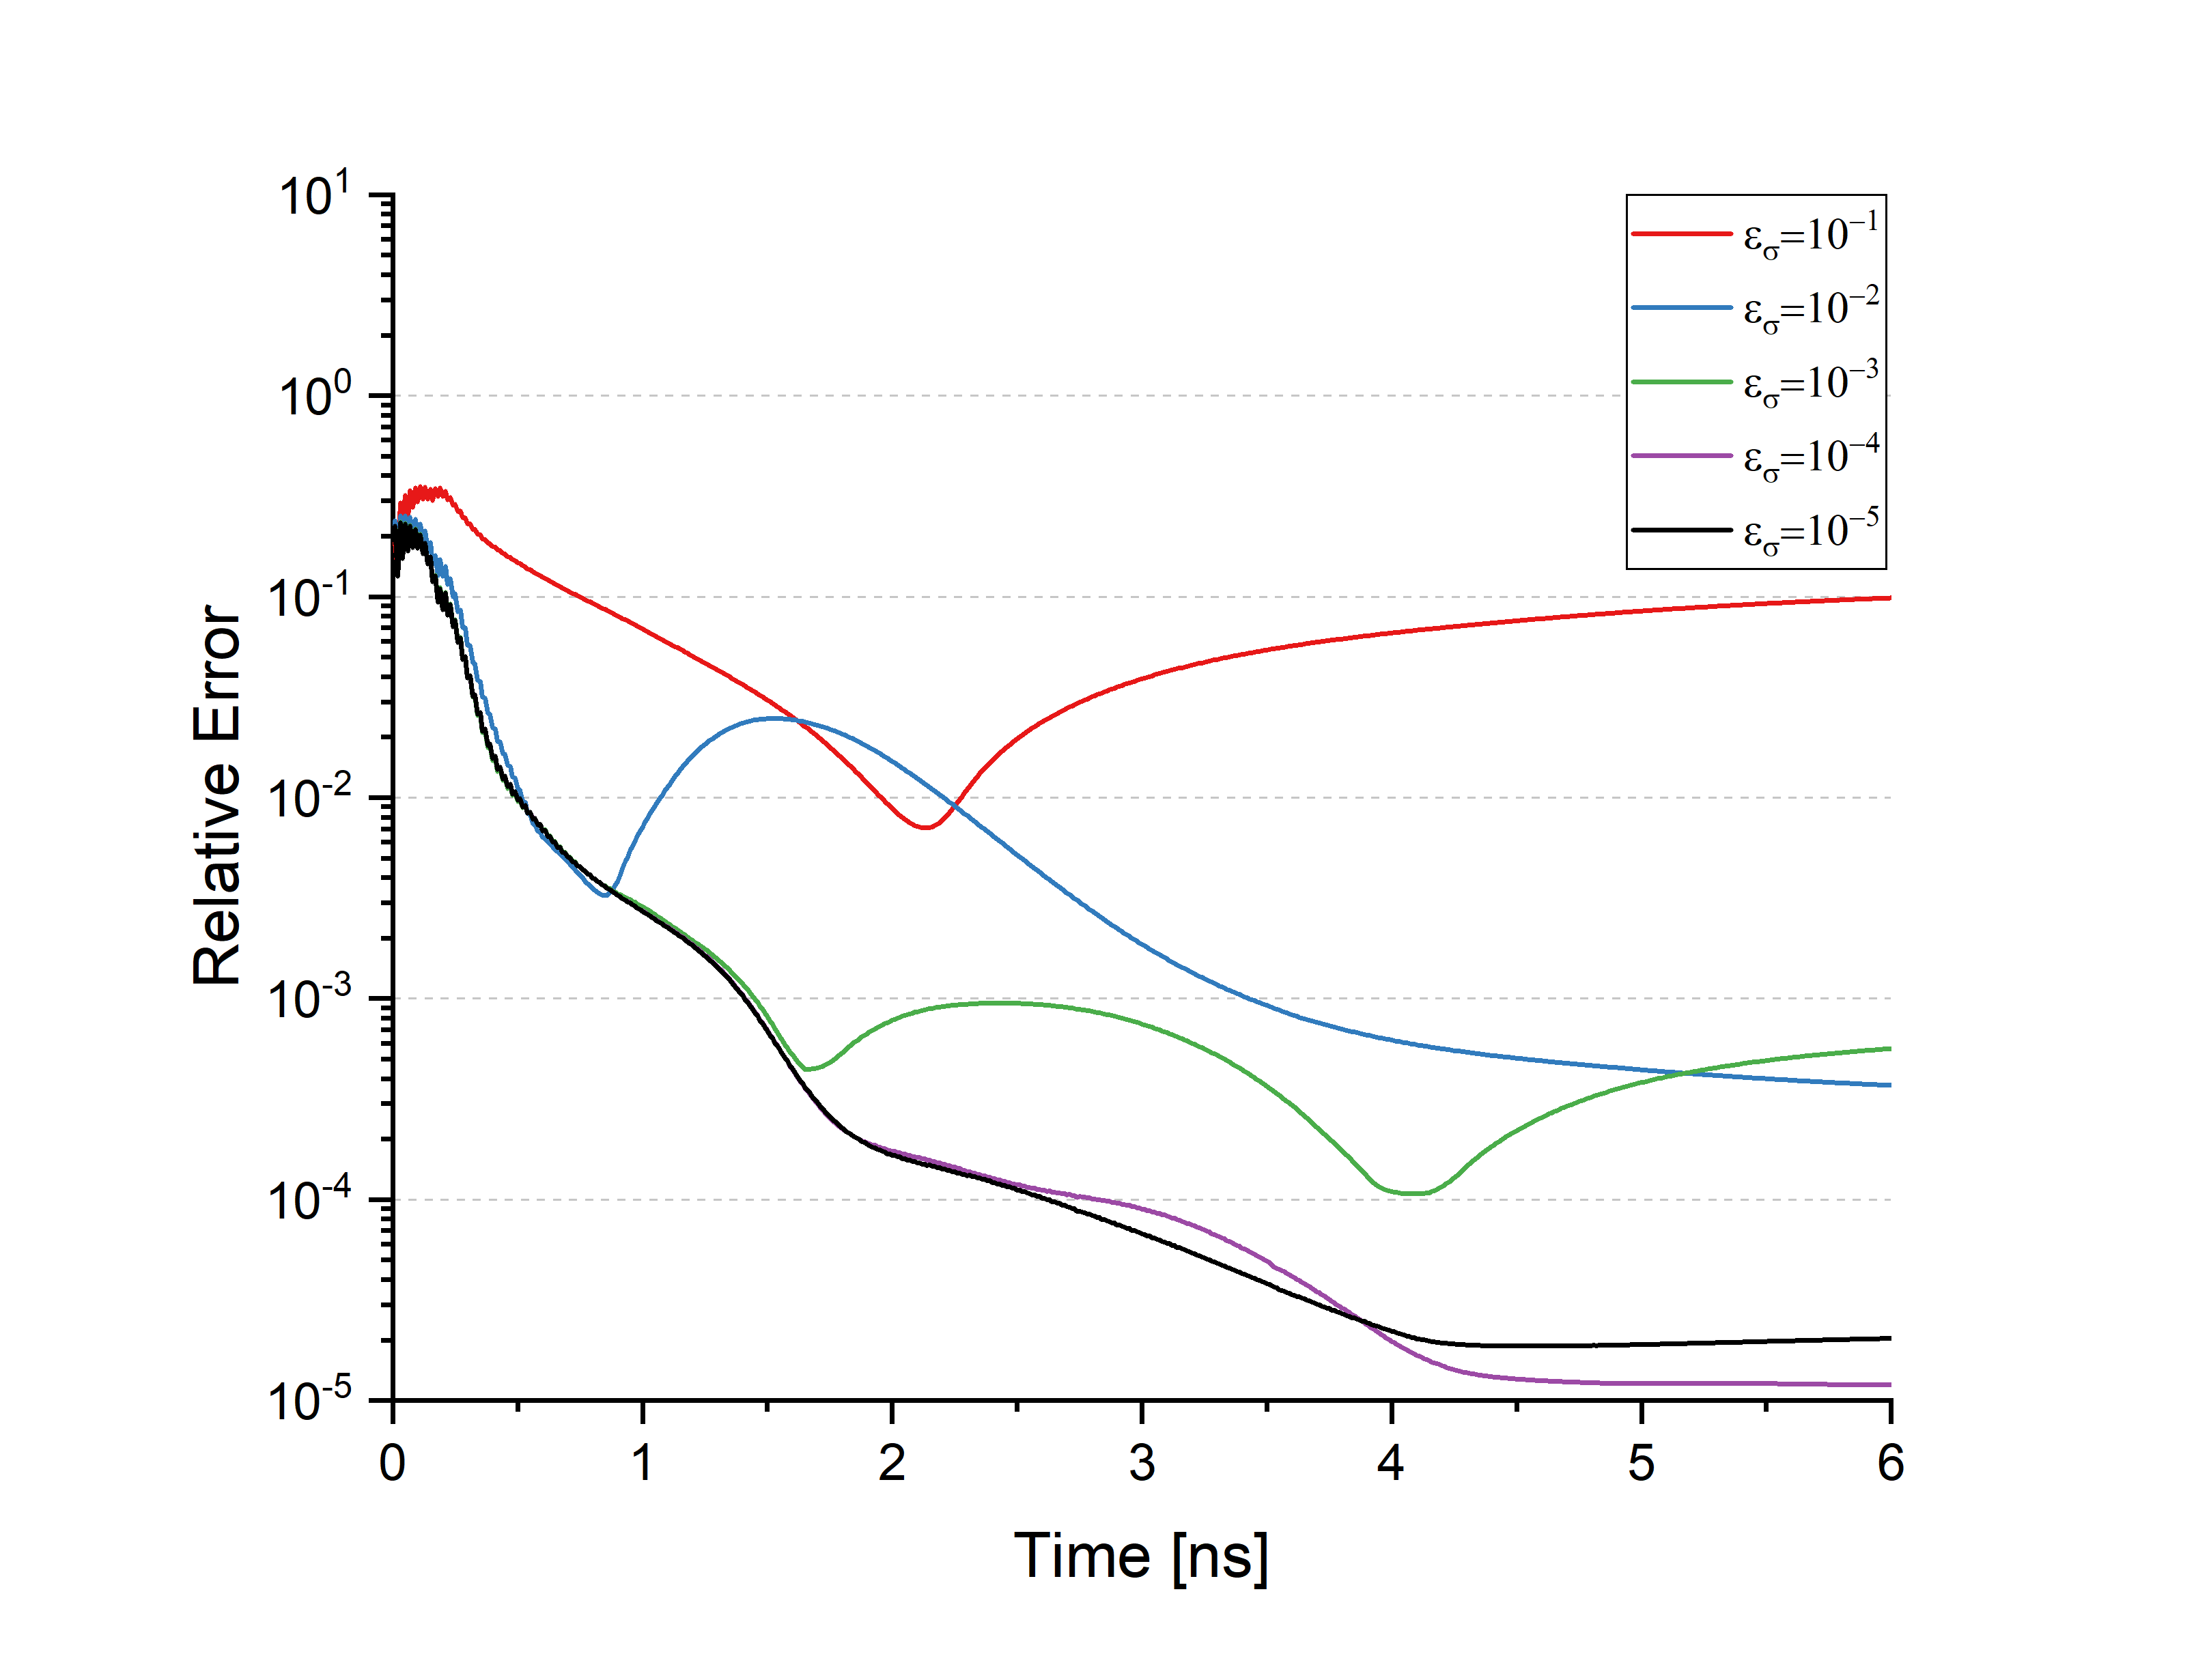
\includegraphics[width=0.475\textwidth]{GR_bc1000-t001_qdf1000-t002_Tavg_grey_fg_bg.png}}
		\subfloat[Energy density relative error using approximate $f_g$ and reference $E_g$ \label{subfig:GR_bc1000-t001_qdf1000-t002_Eavg_grey_fg}]{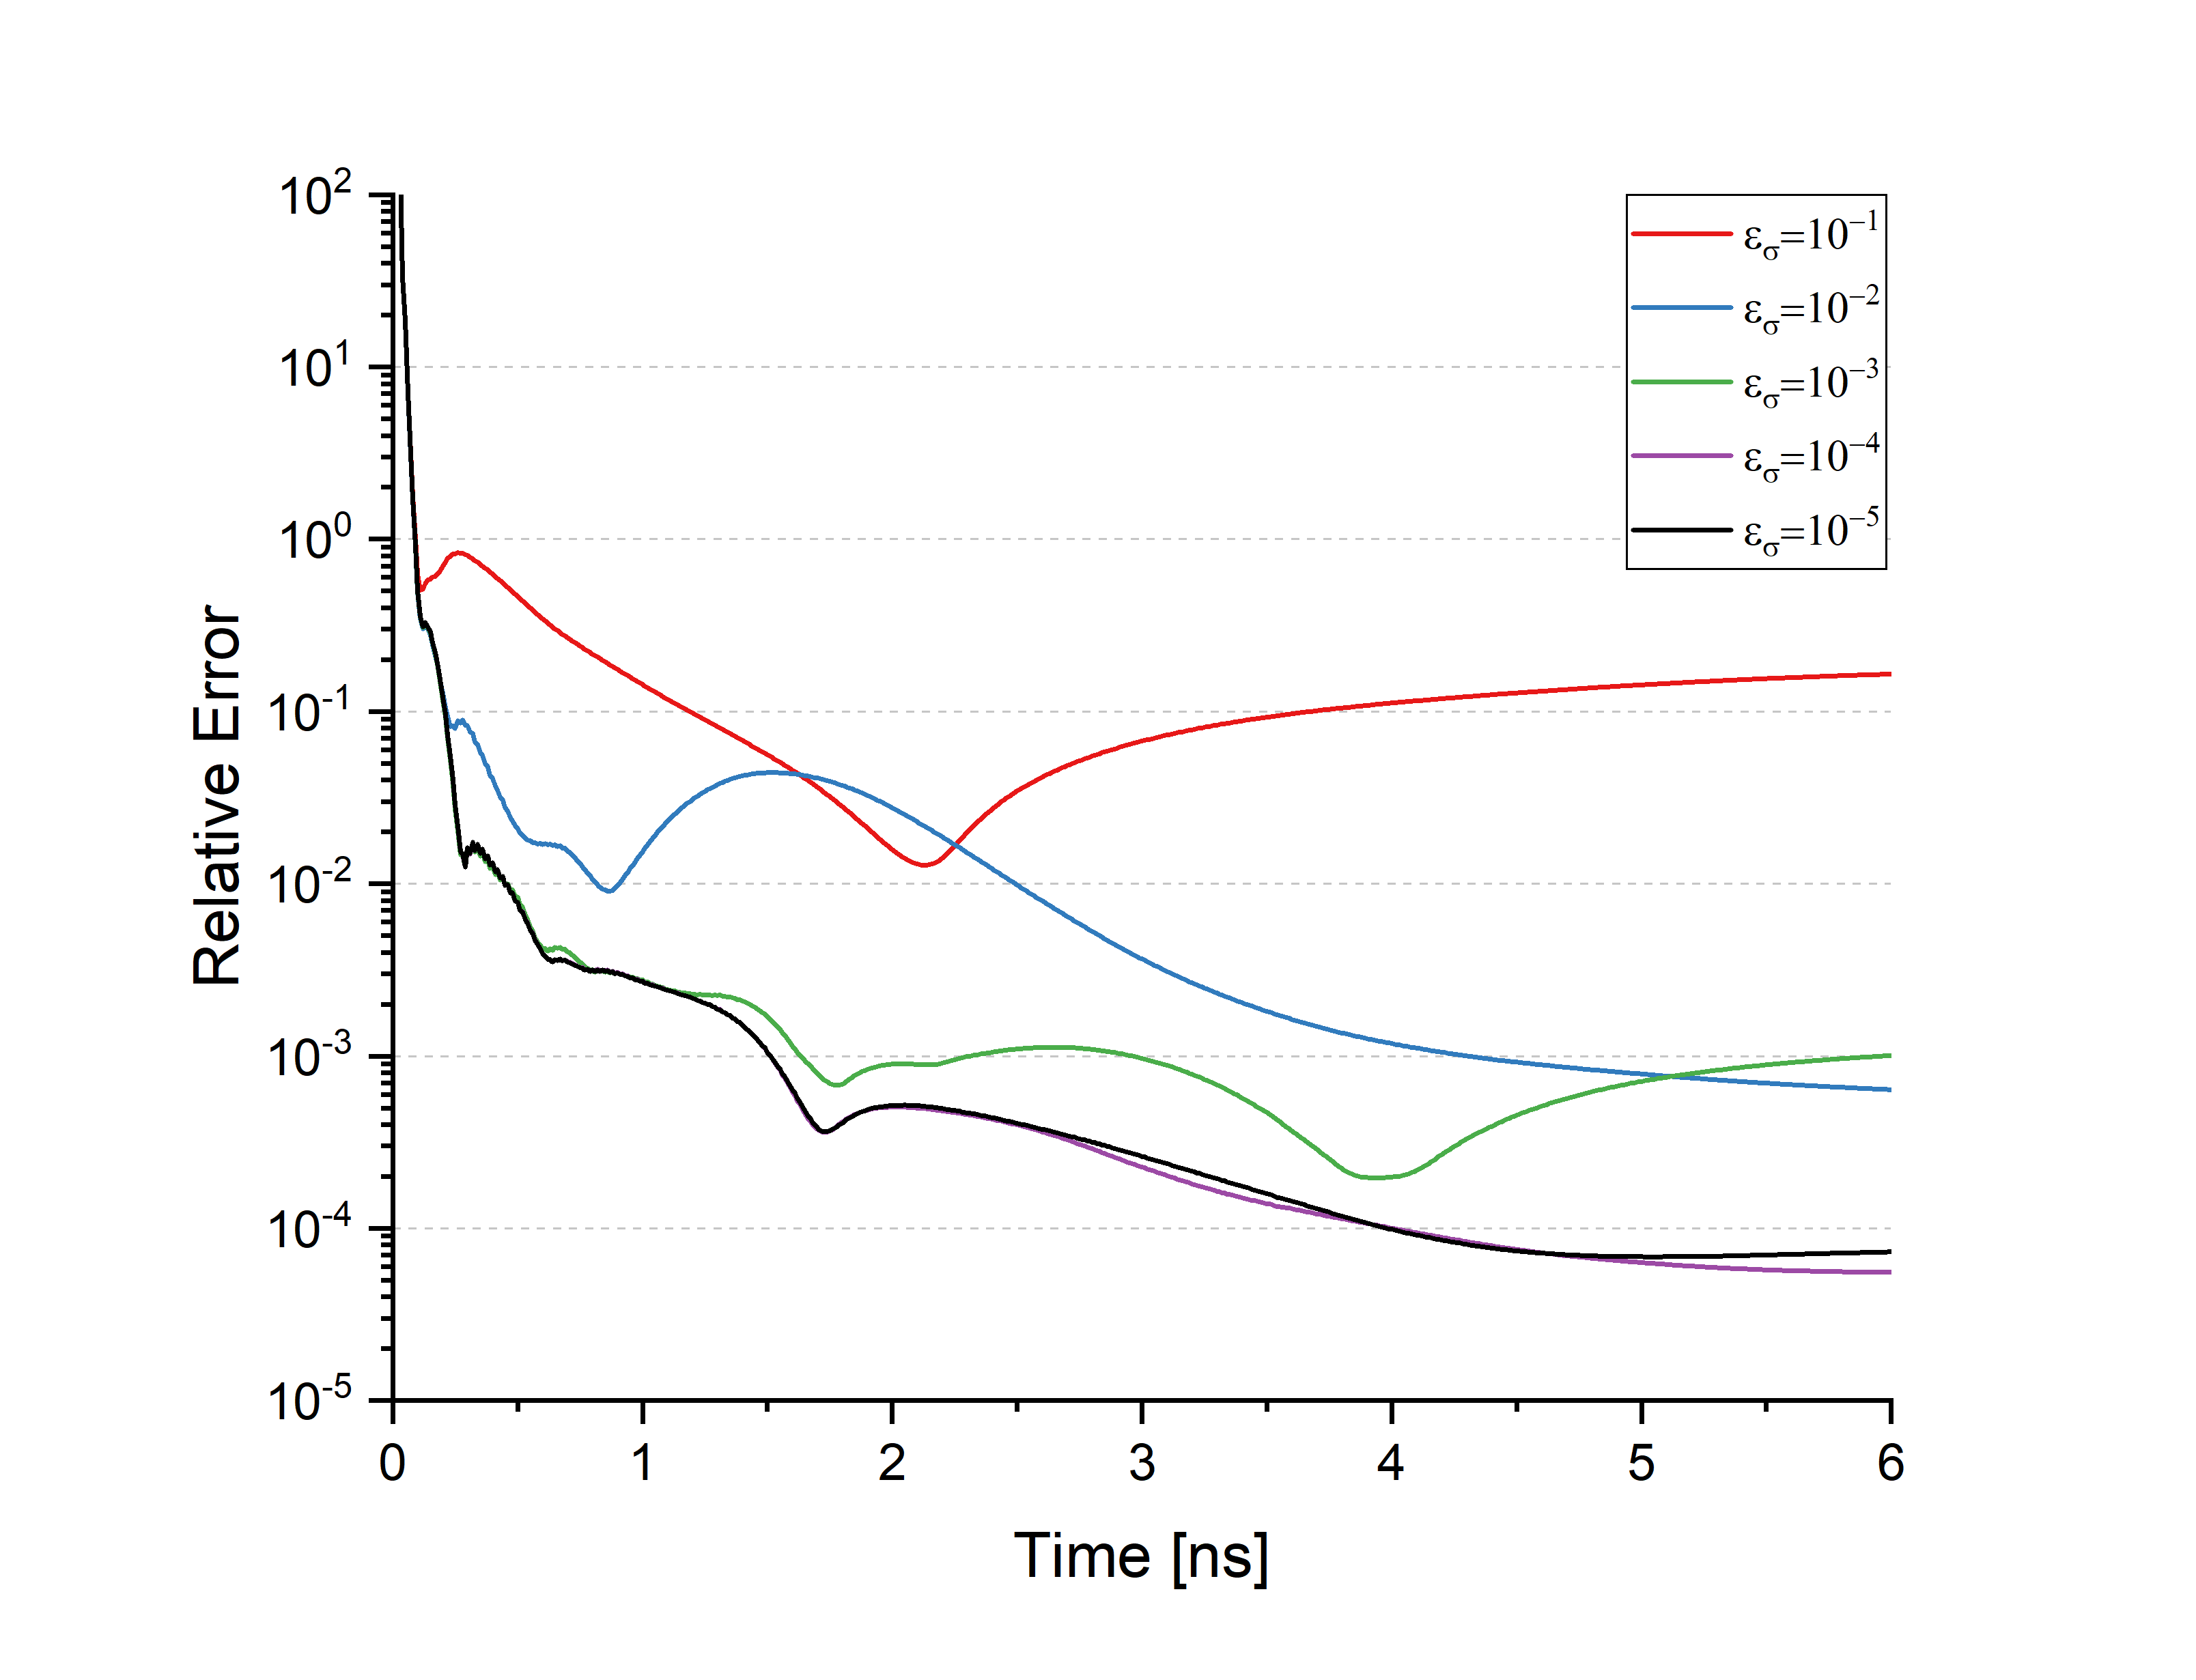
\includegraphics[width=0.475\textwidth]{GR_bc1000-t001_qdf1000-t002_Eavg_grey_fg_bg.png}}\\
		\subfloat[Temperature relative error using reference $f_g$ and approximate $E_g$ \label{subfig:GR_bc1000-t001_qdf1000-t002_Tavg_grey_Eg}]{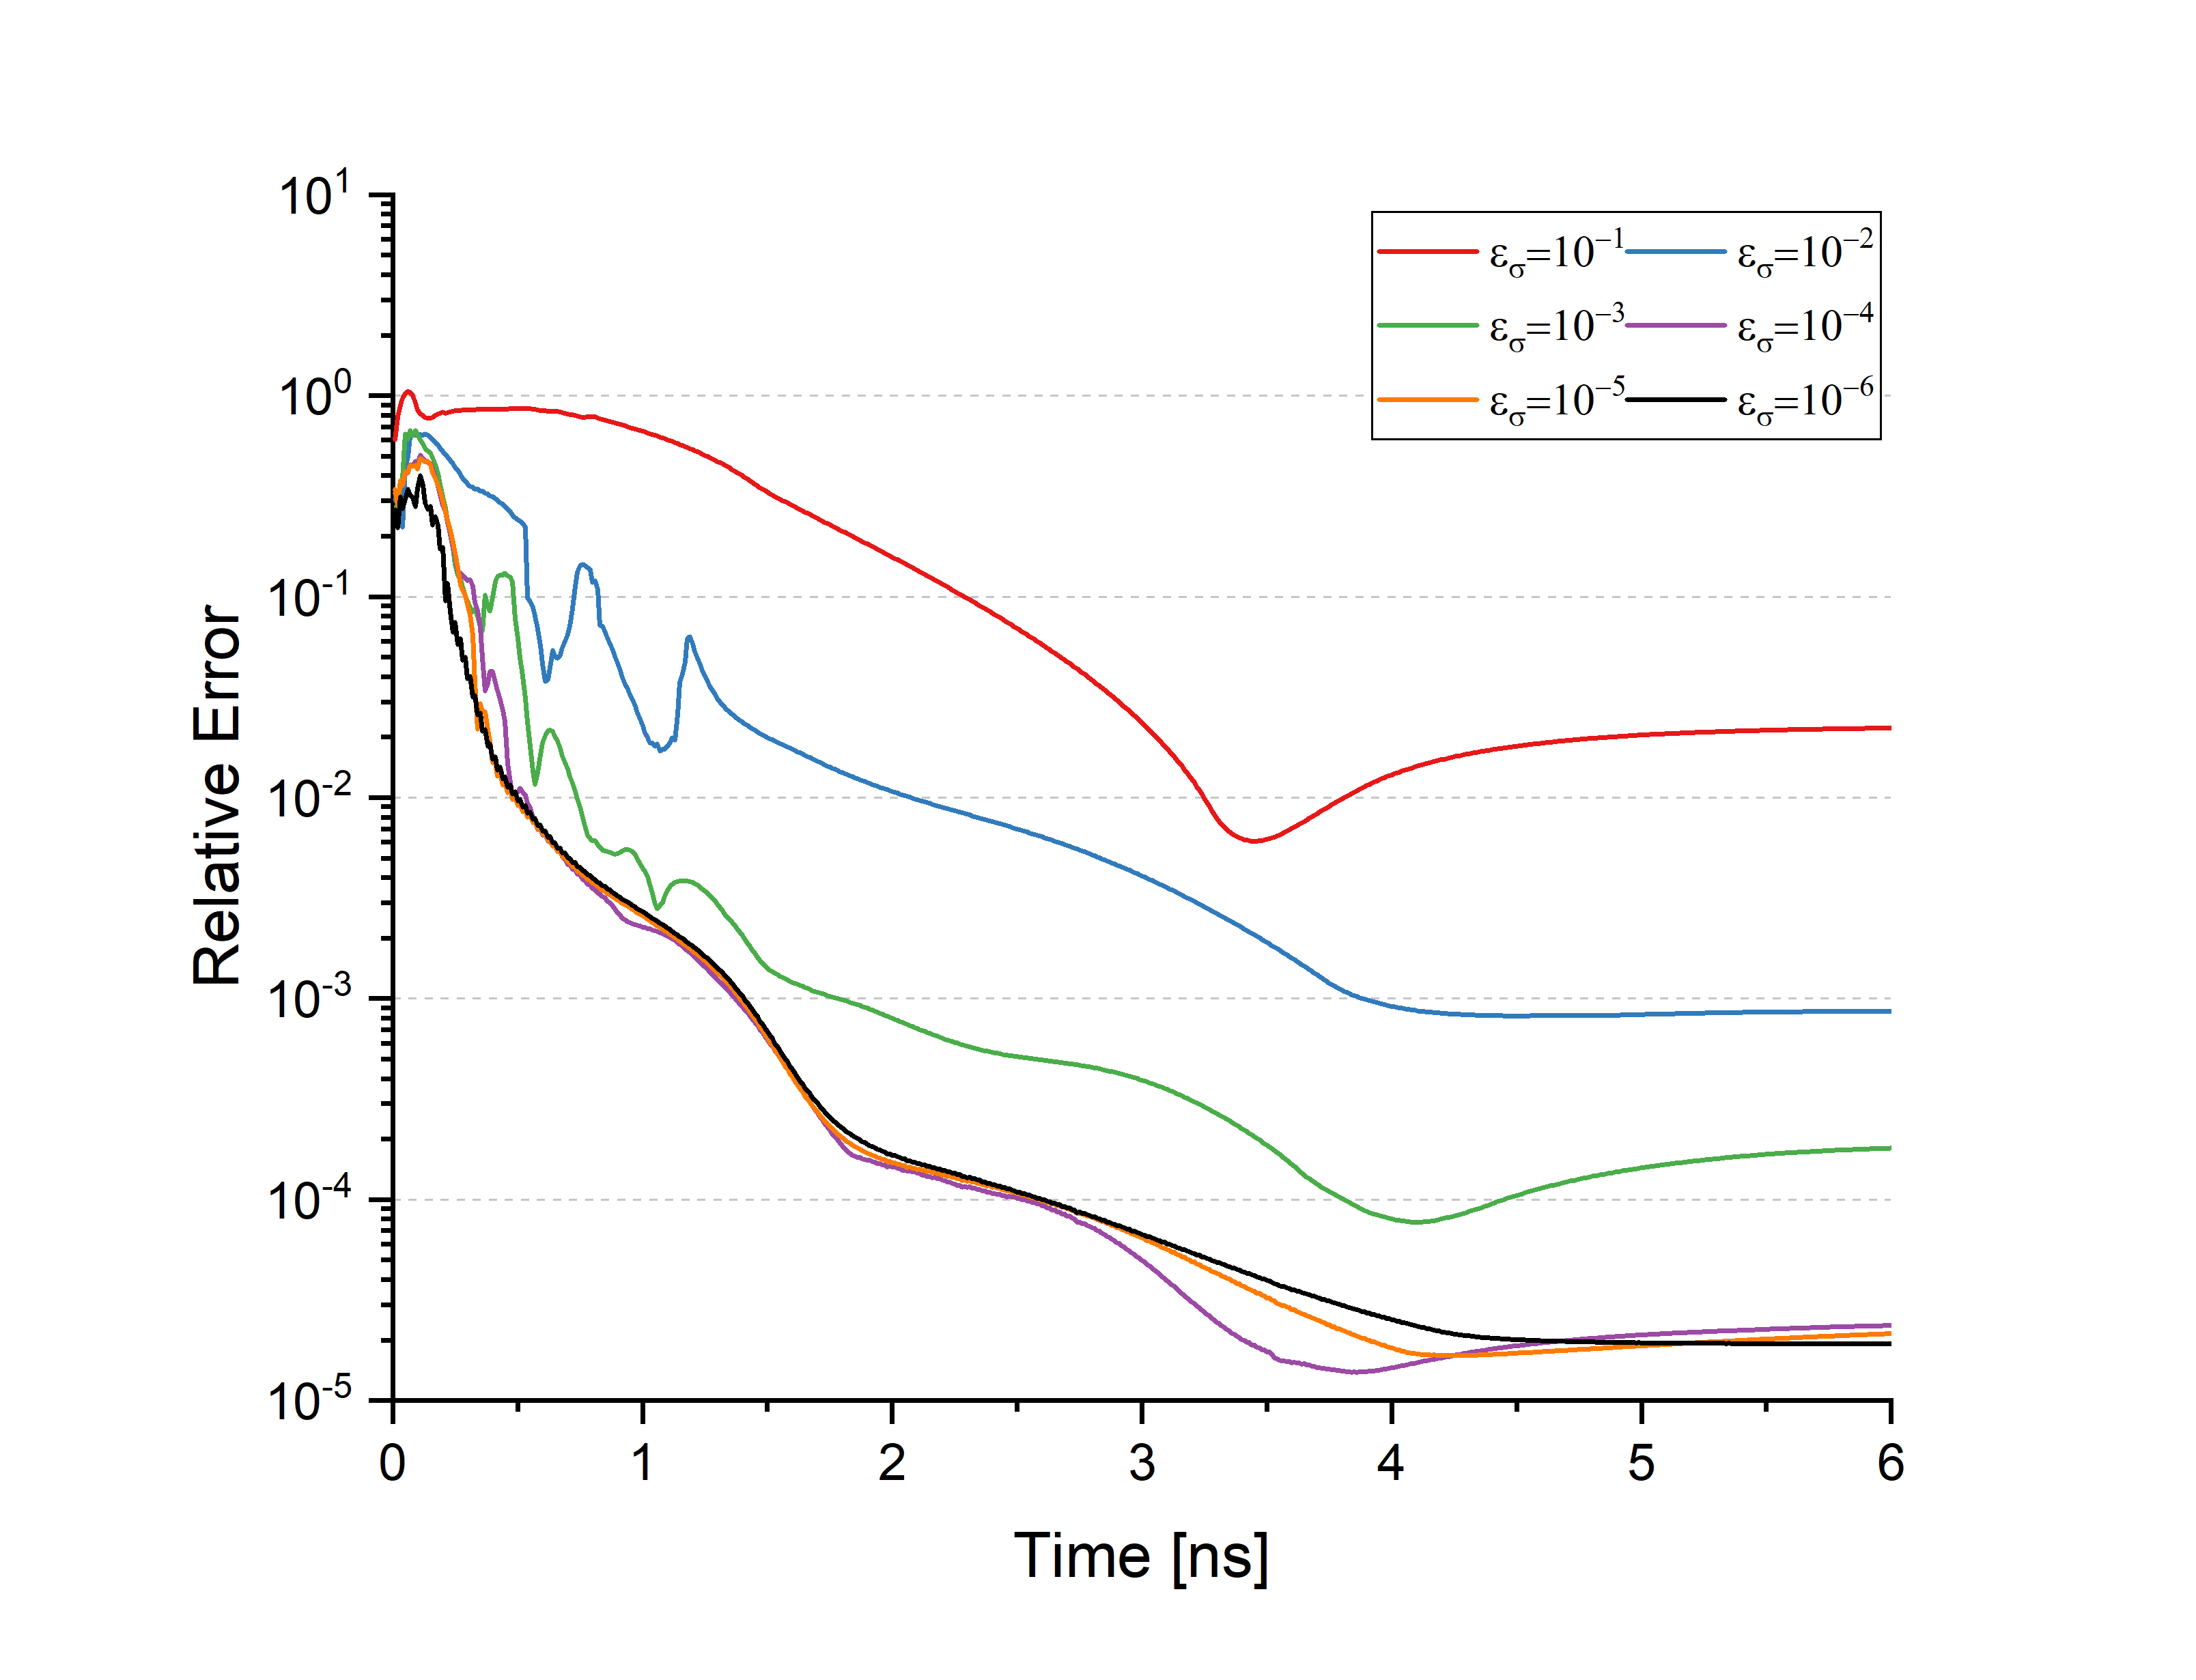
\includegraphics[width=0.475\textwidth]{GR_bc1000-t001_qdf1000-t002_Tavg_grey_Eg_bg.png}}
		\subfloat[Energy density relative error using reference $f_g$ and approximate $E_g$ \label{subfig:GR_bc1000-t001_qdf1000-t002_Eavg_grey_Eg}]{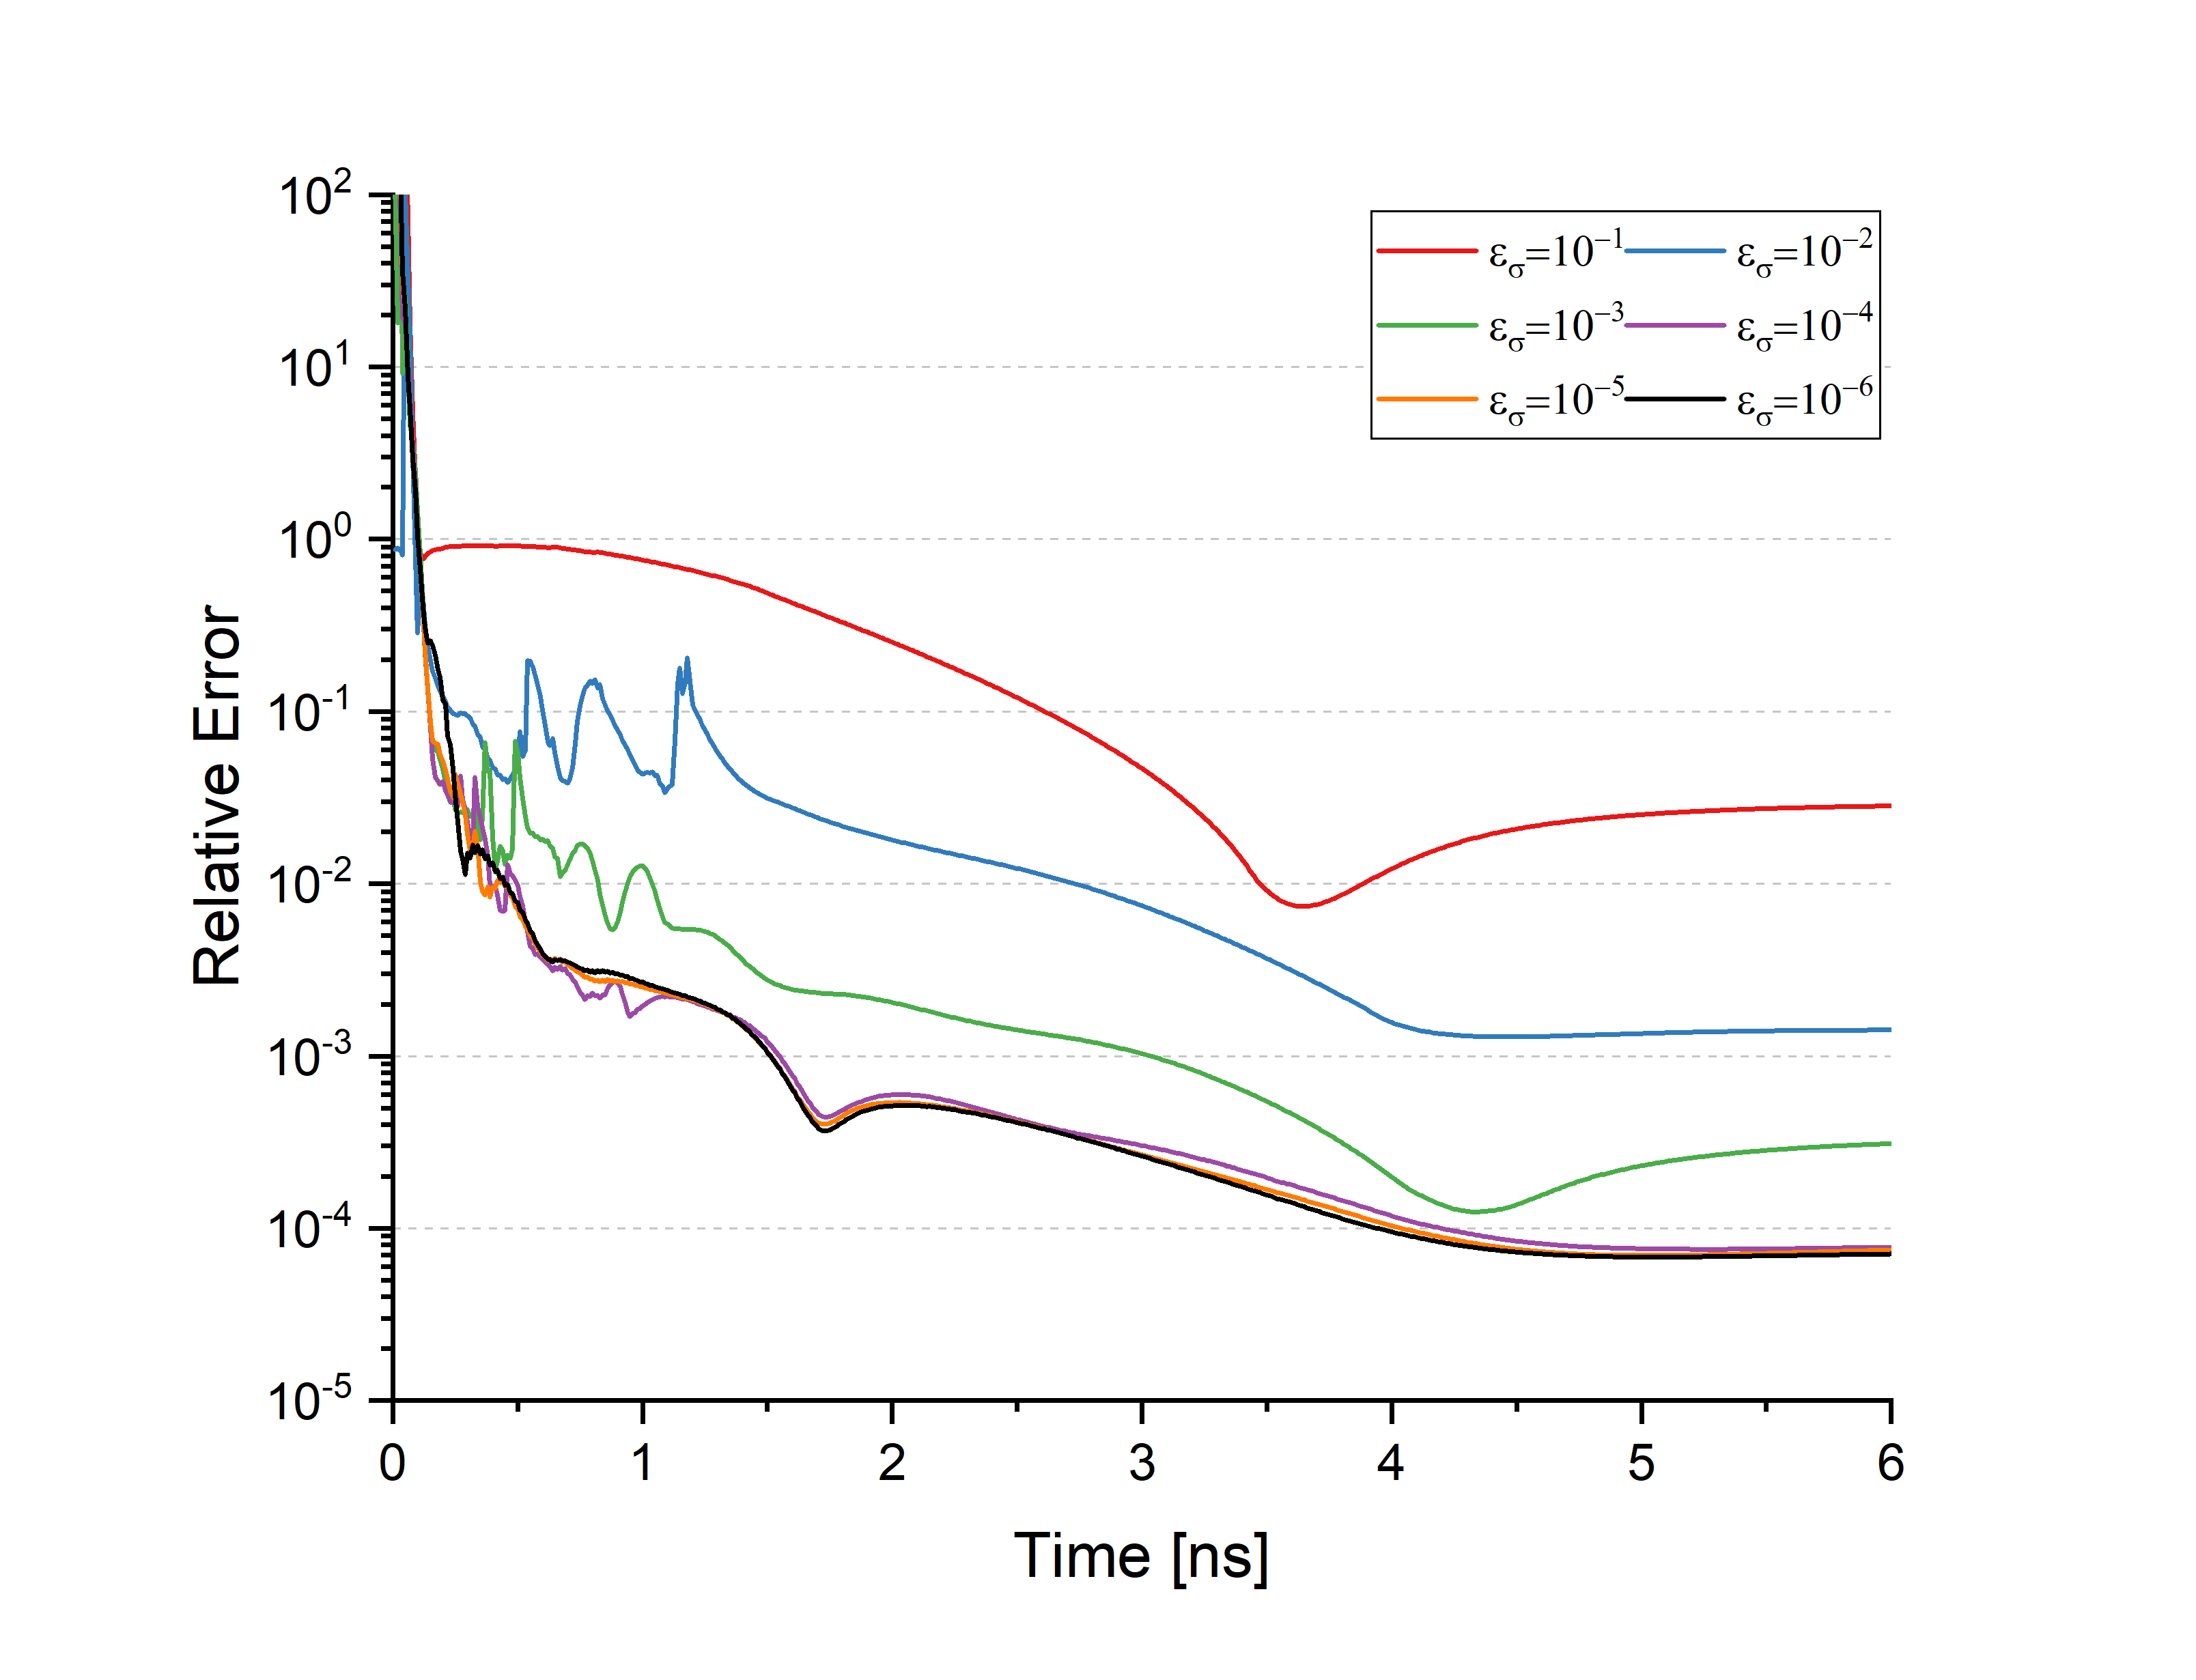
\includegraphics[width=0.475\textwidth]{GR_bc1000-t001_qdf1000-t002_Eavg_grey_Eg_bg.png}}\\
		\subfloat[Temperature relative error using approximate \newline $f_g$ and approximate $E_g$ \label{subfig:GR_bc1000-t001_qdf1000-t002_Tavg_grey_E-fg}]{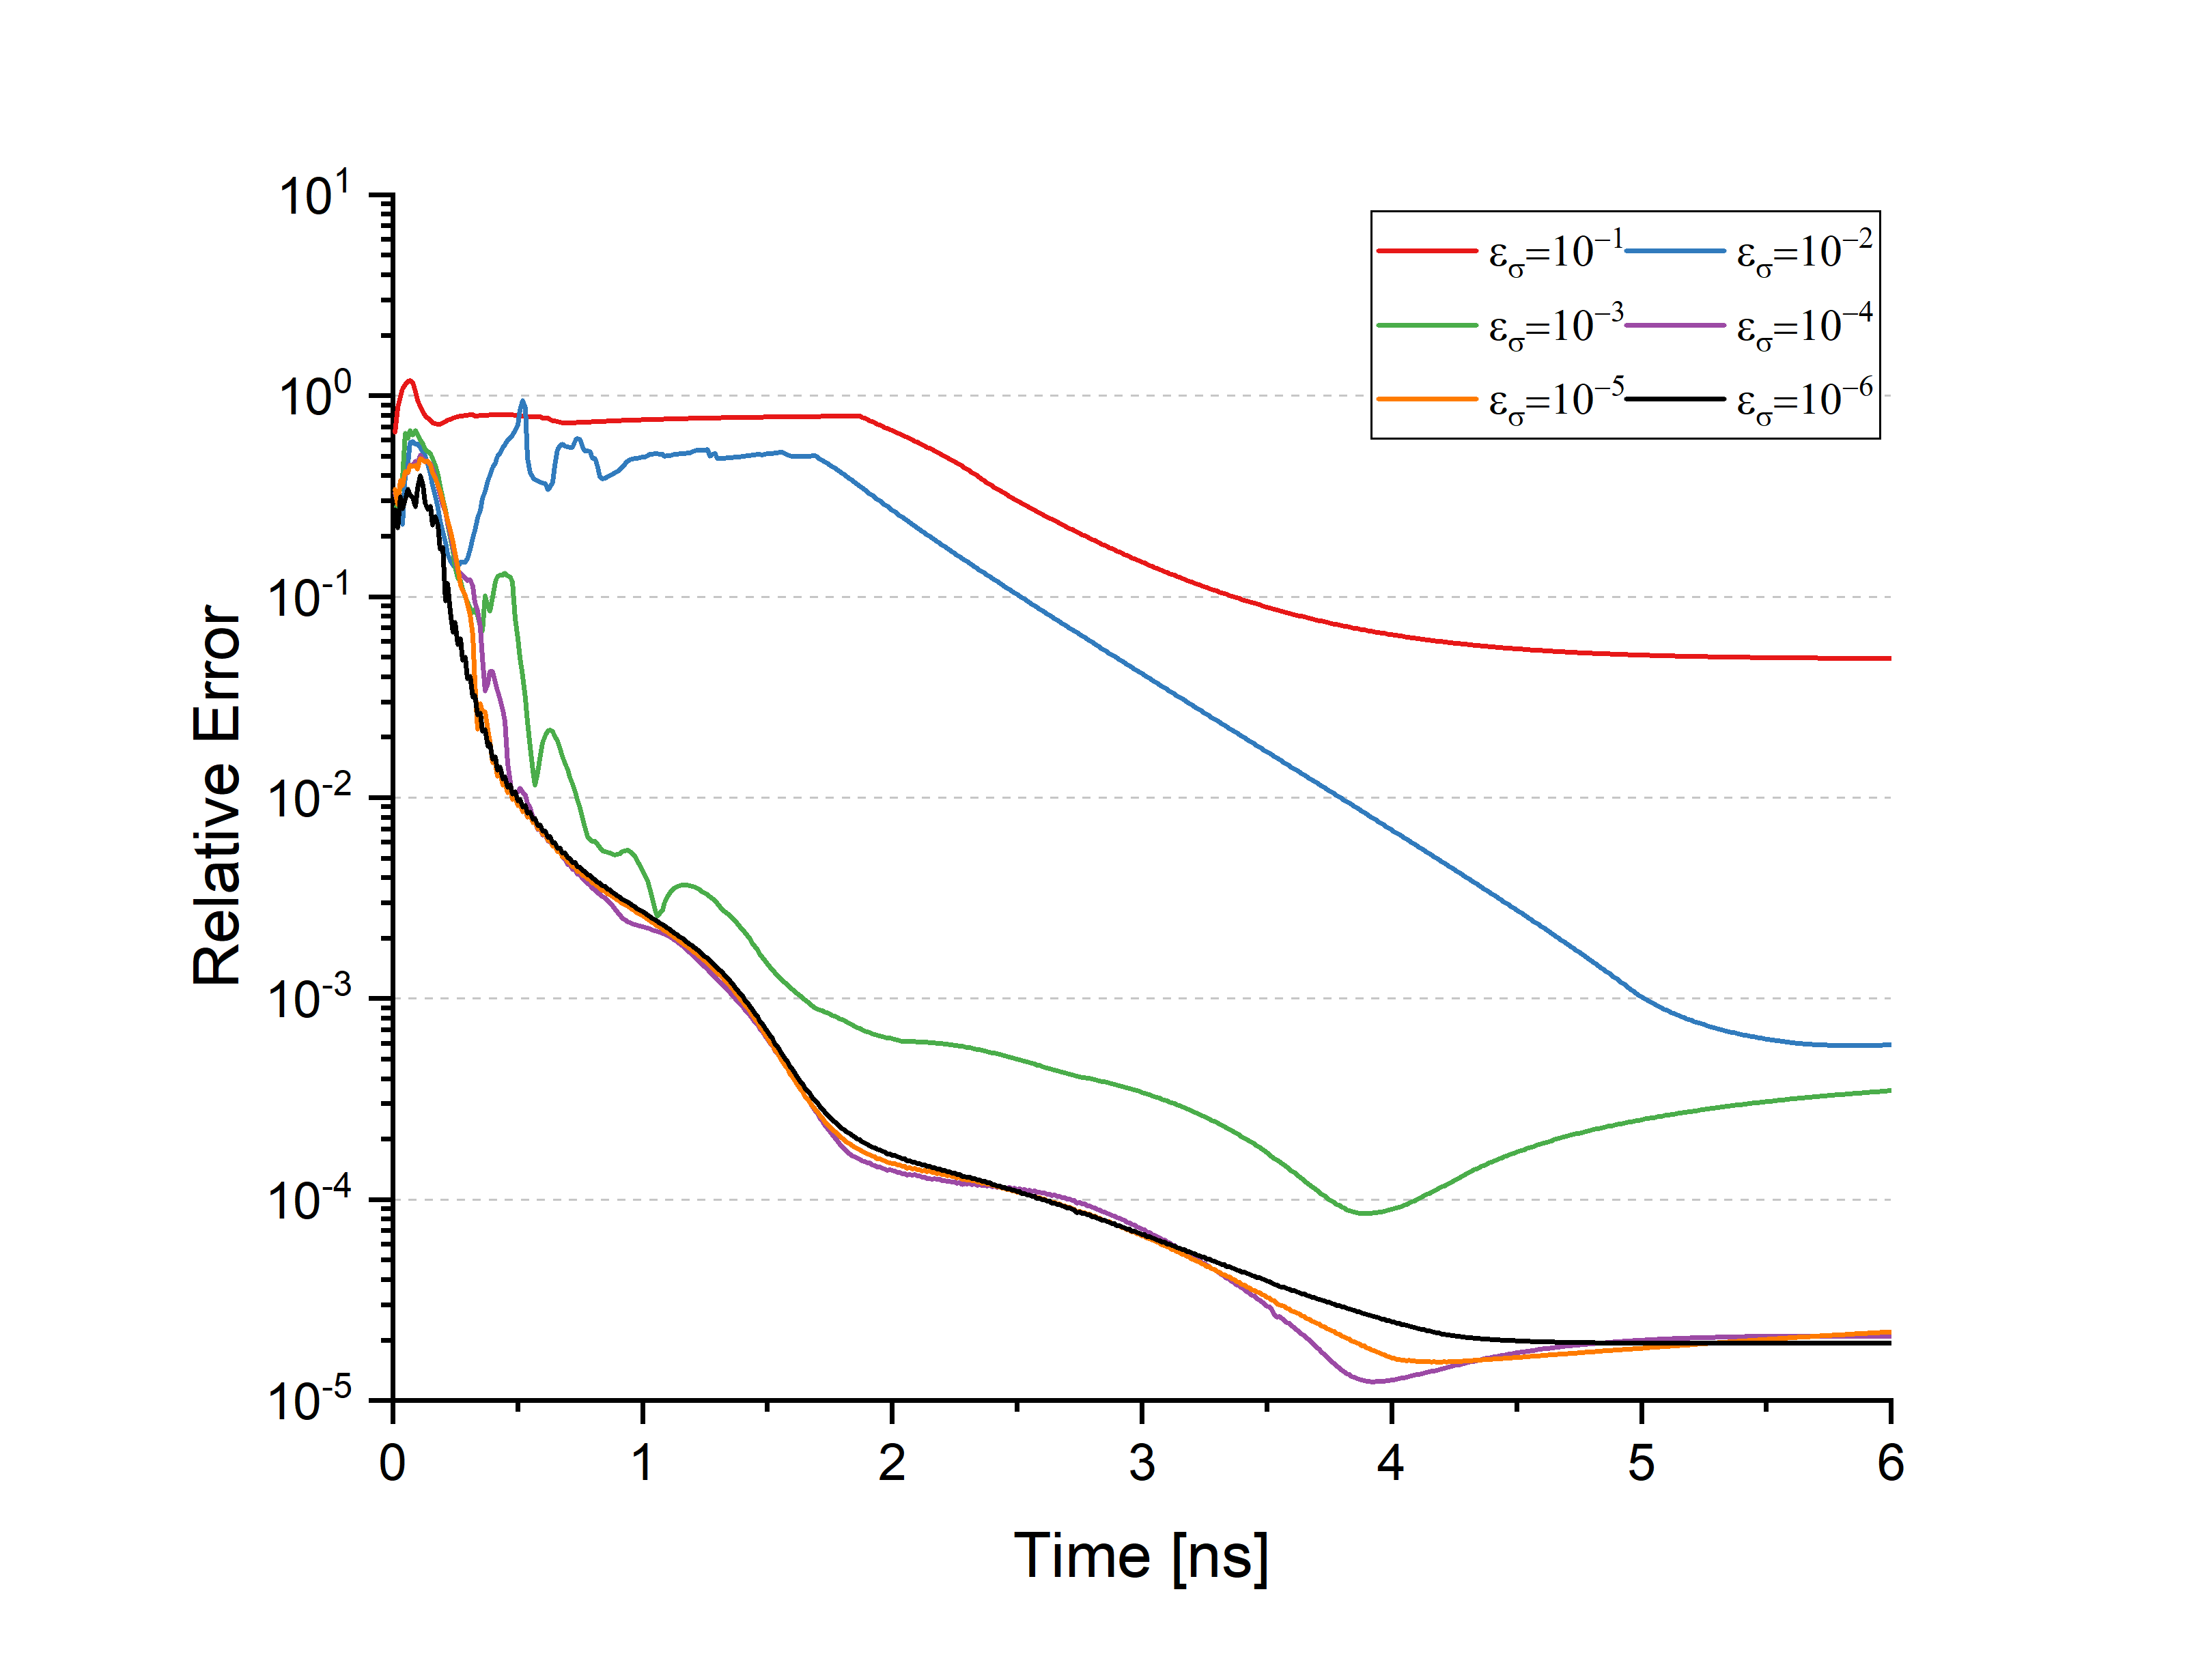
\includegraphics[width=0.475\textwidth]{GR_bc1000-t001_qdf1000-t002_Tavg_grey_E-fg_bg.png}}
		\subfloat[Energy density relative error using approximate $f_g$ and approximate $E_g$ \label{subfig:GR_bc1000-t001_qdf1000-t002_Eavg_grey_E-fg}]{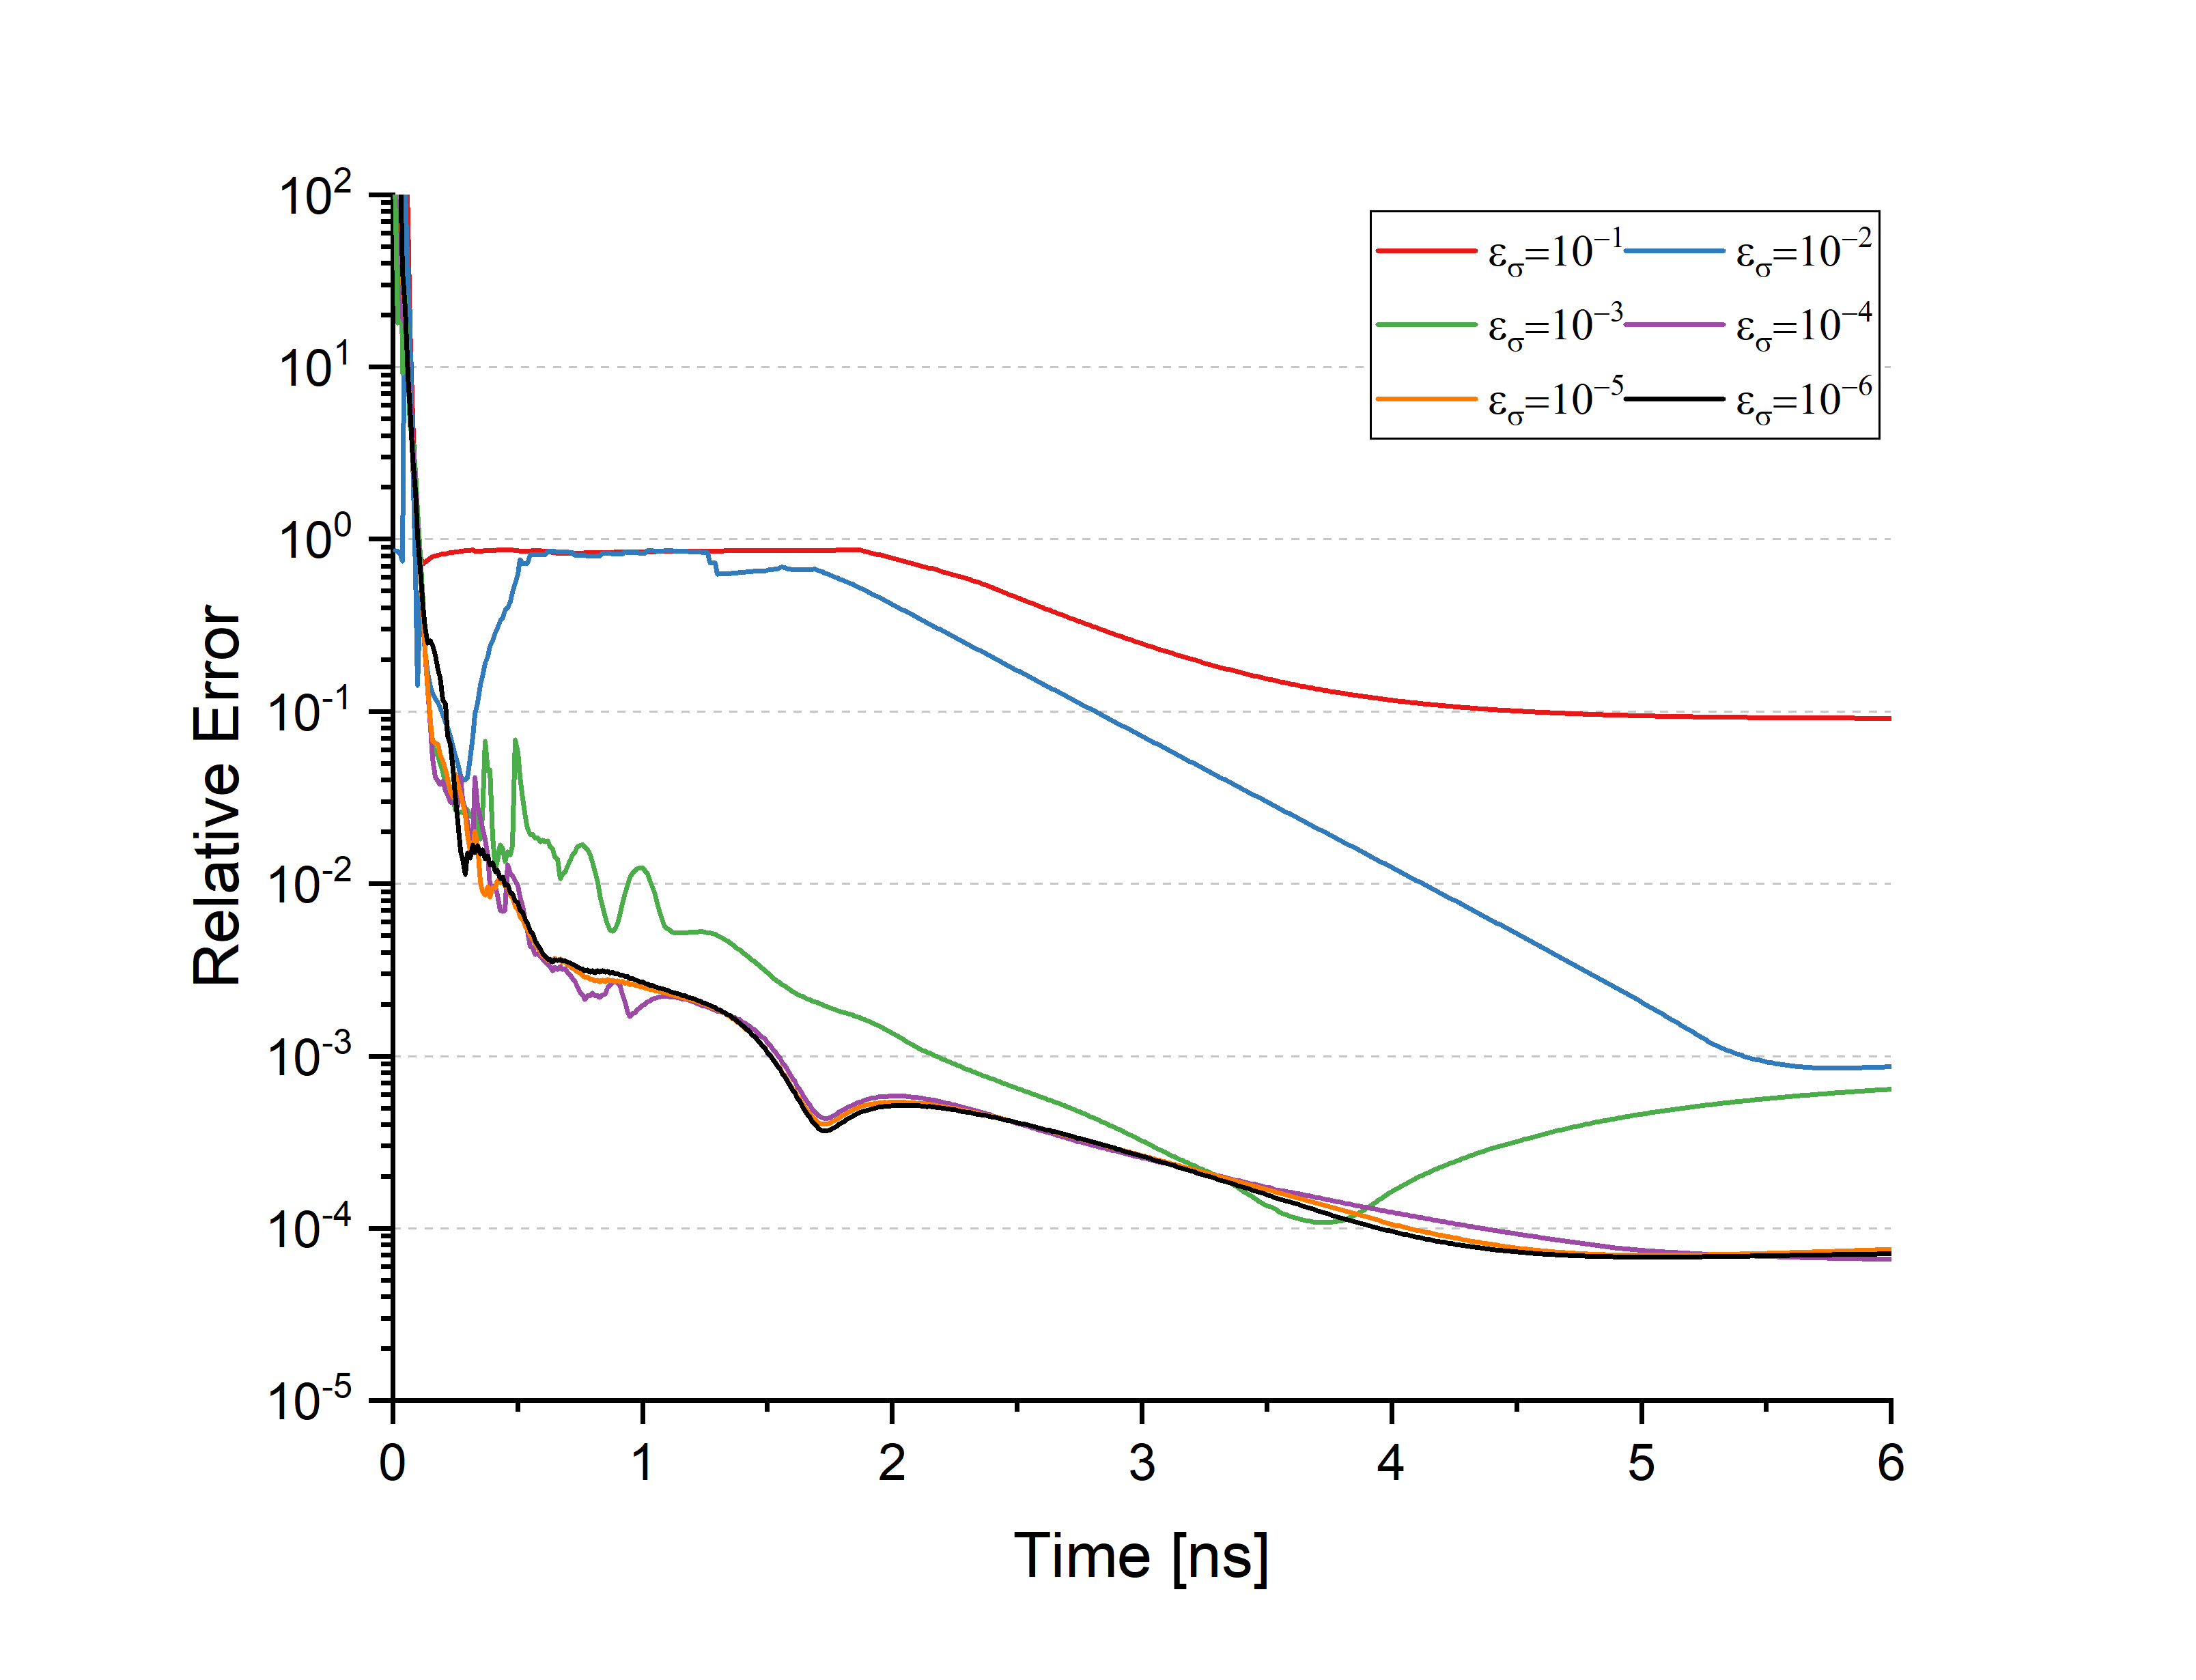
\includegraphics[width=0.475\textwidth]{GR_bc1000-t001_qdf1000-t002_Eavg_grey_E-fg_bg.png}}
		\caption{\label{fig:errors_dt-0.01_grey}
			Relative error in the $L_1$-norm of GLOQD-POD solutions computed with $\Delta t\! =\! 1 \! \times \! 10^{-2}$~ns
			versus the reference TRT solution. Data for the GLOQD-POD model is generated with $\Delta t\! =\! 2 \! \times\!  10^{-2}$ ns. }
	\end{figure}
	
	
	\begin{figure}[ht!]
		\centering
		\subfloat[Temperature relative error using approximate \newline $f_g$ and reference $E_g$ \label{subfig:GR_bc1000-t0005_qdf1000-t002_Tavg_grey_fg}]{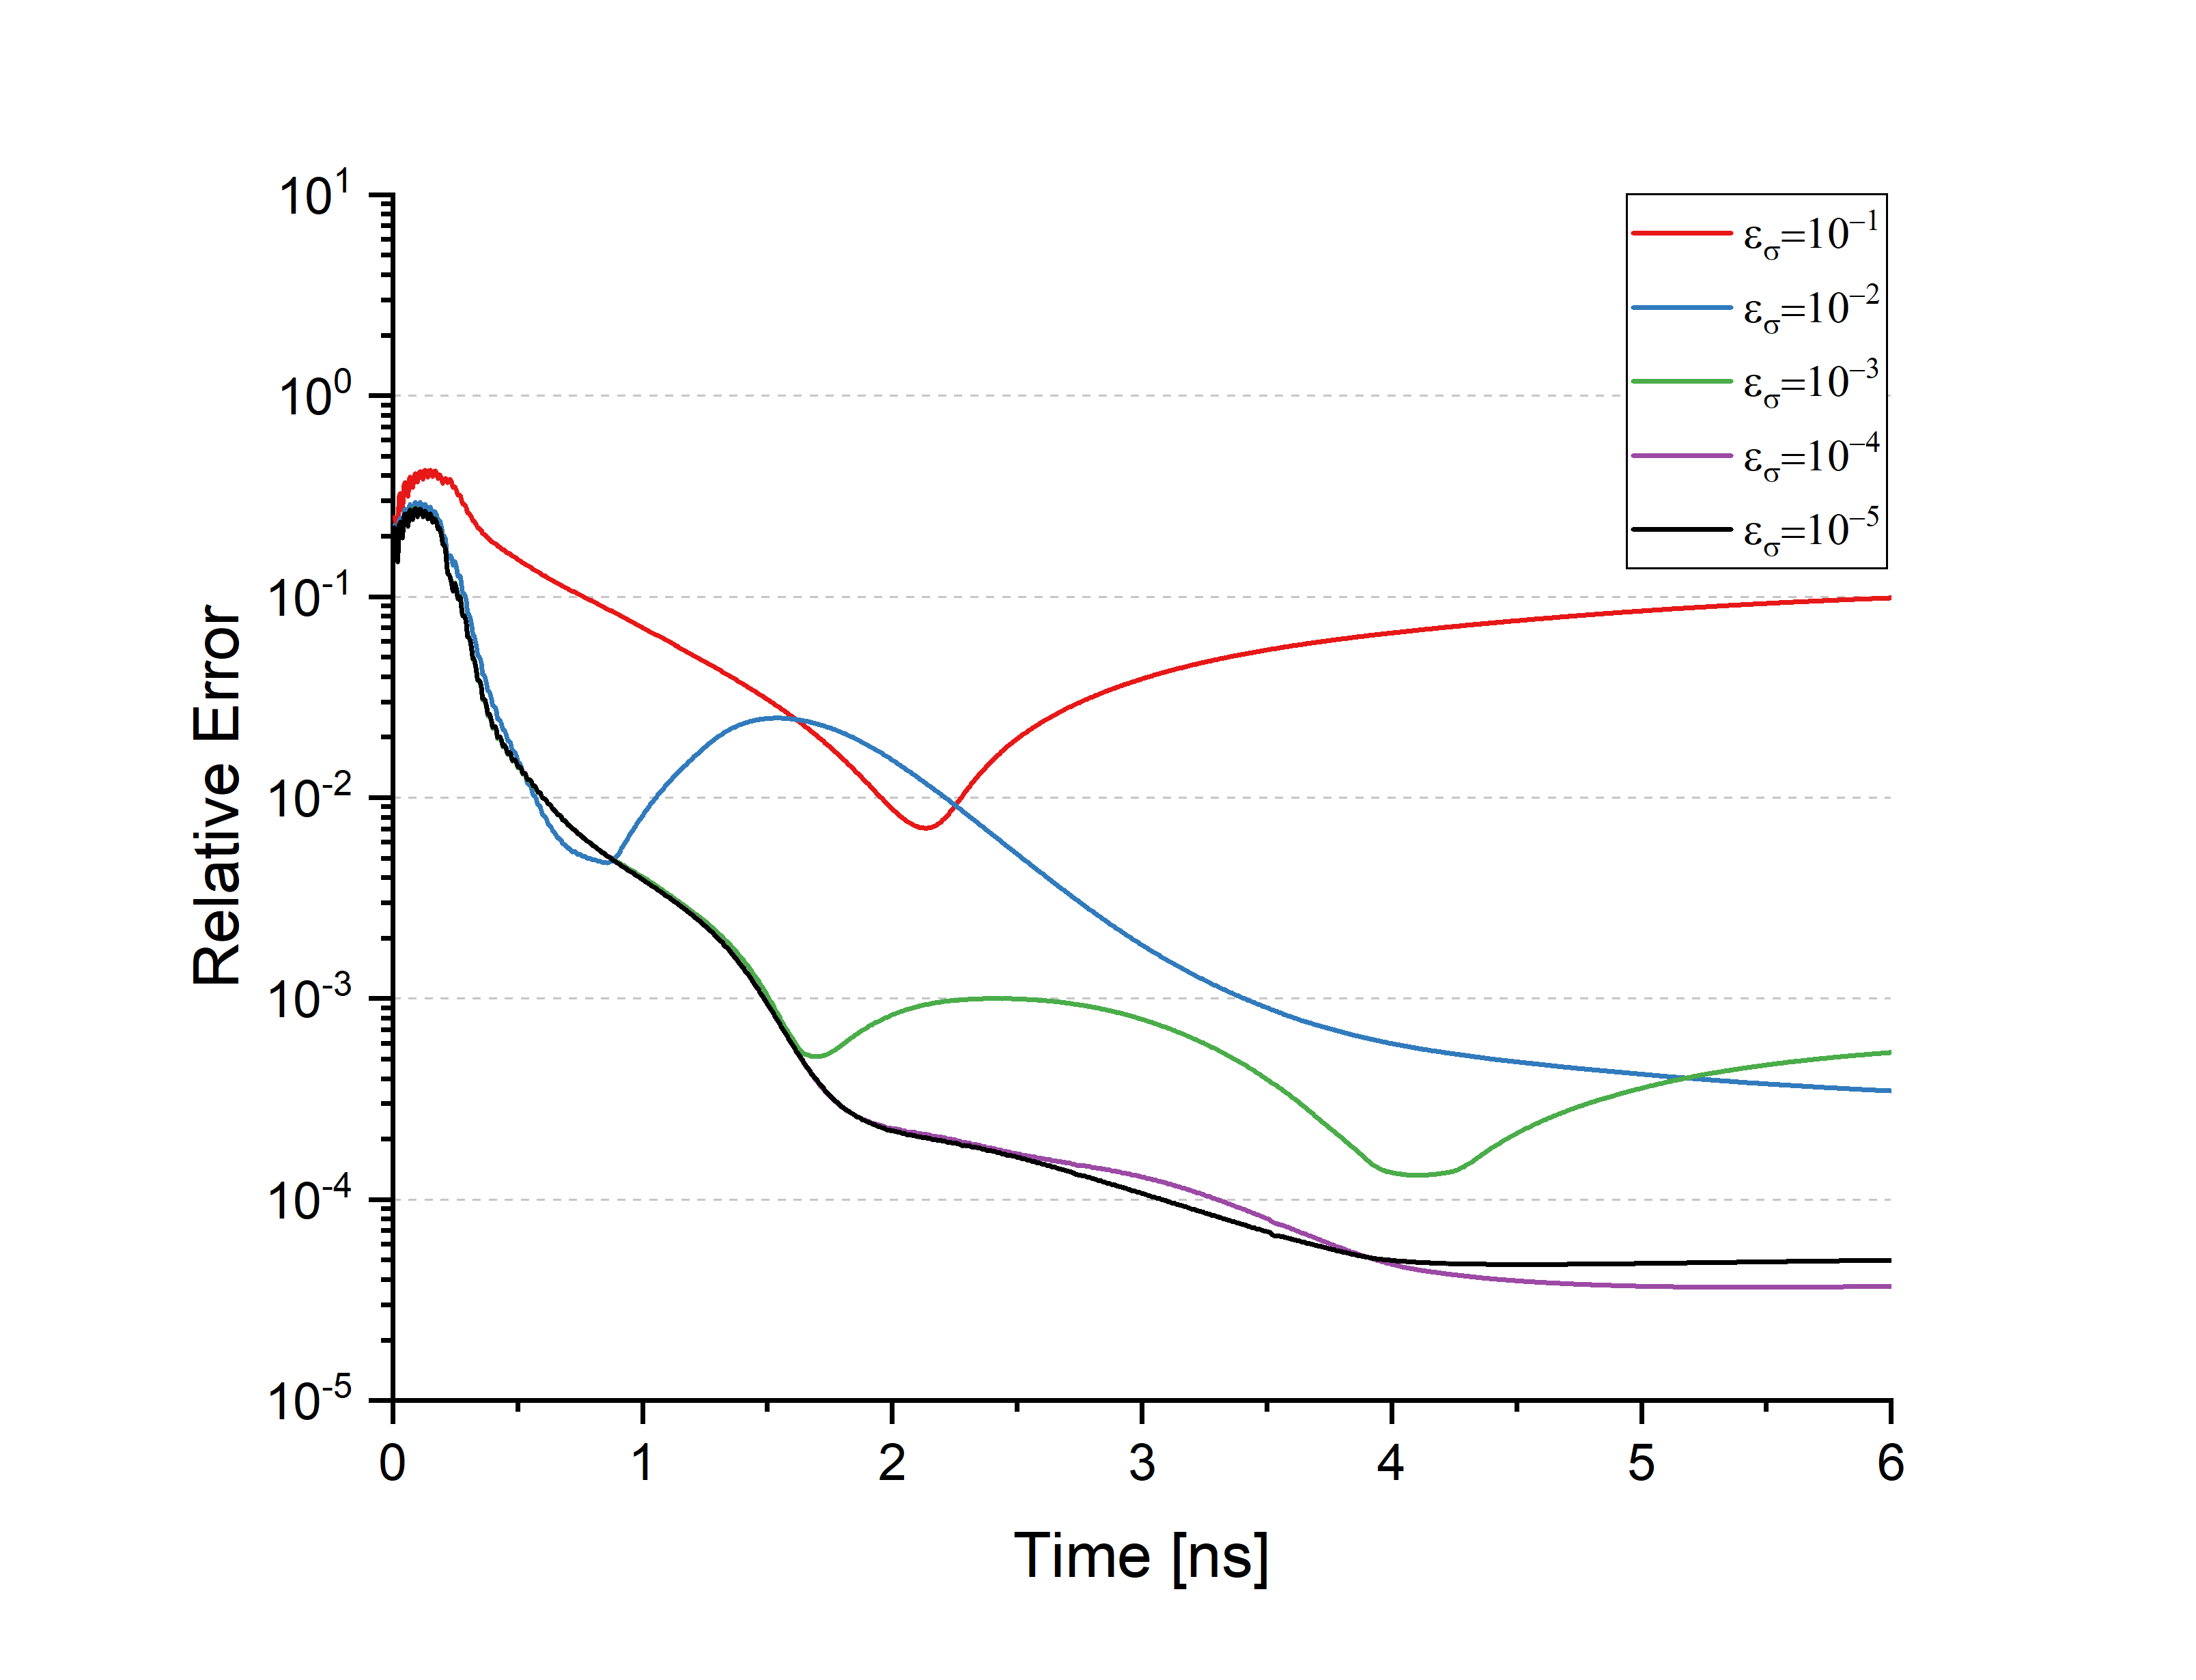
\includegraphics[width=0.475\textwidth]{GR_bc1000-t0005_qdf1000-t002_Tavg_grey_fg_bg.png}}
		\subfloat[Energy density relative error using approximate $f_g$ and reference $E_g$ \label{subfig:GR_bc1000-t0005_qdf1000-t002_Eavg_grey_fg}]{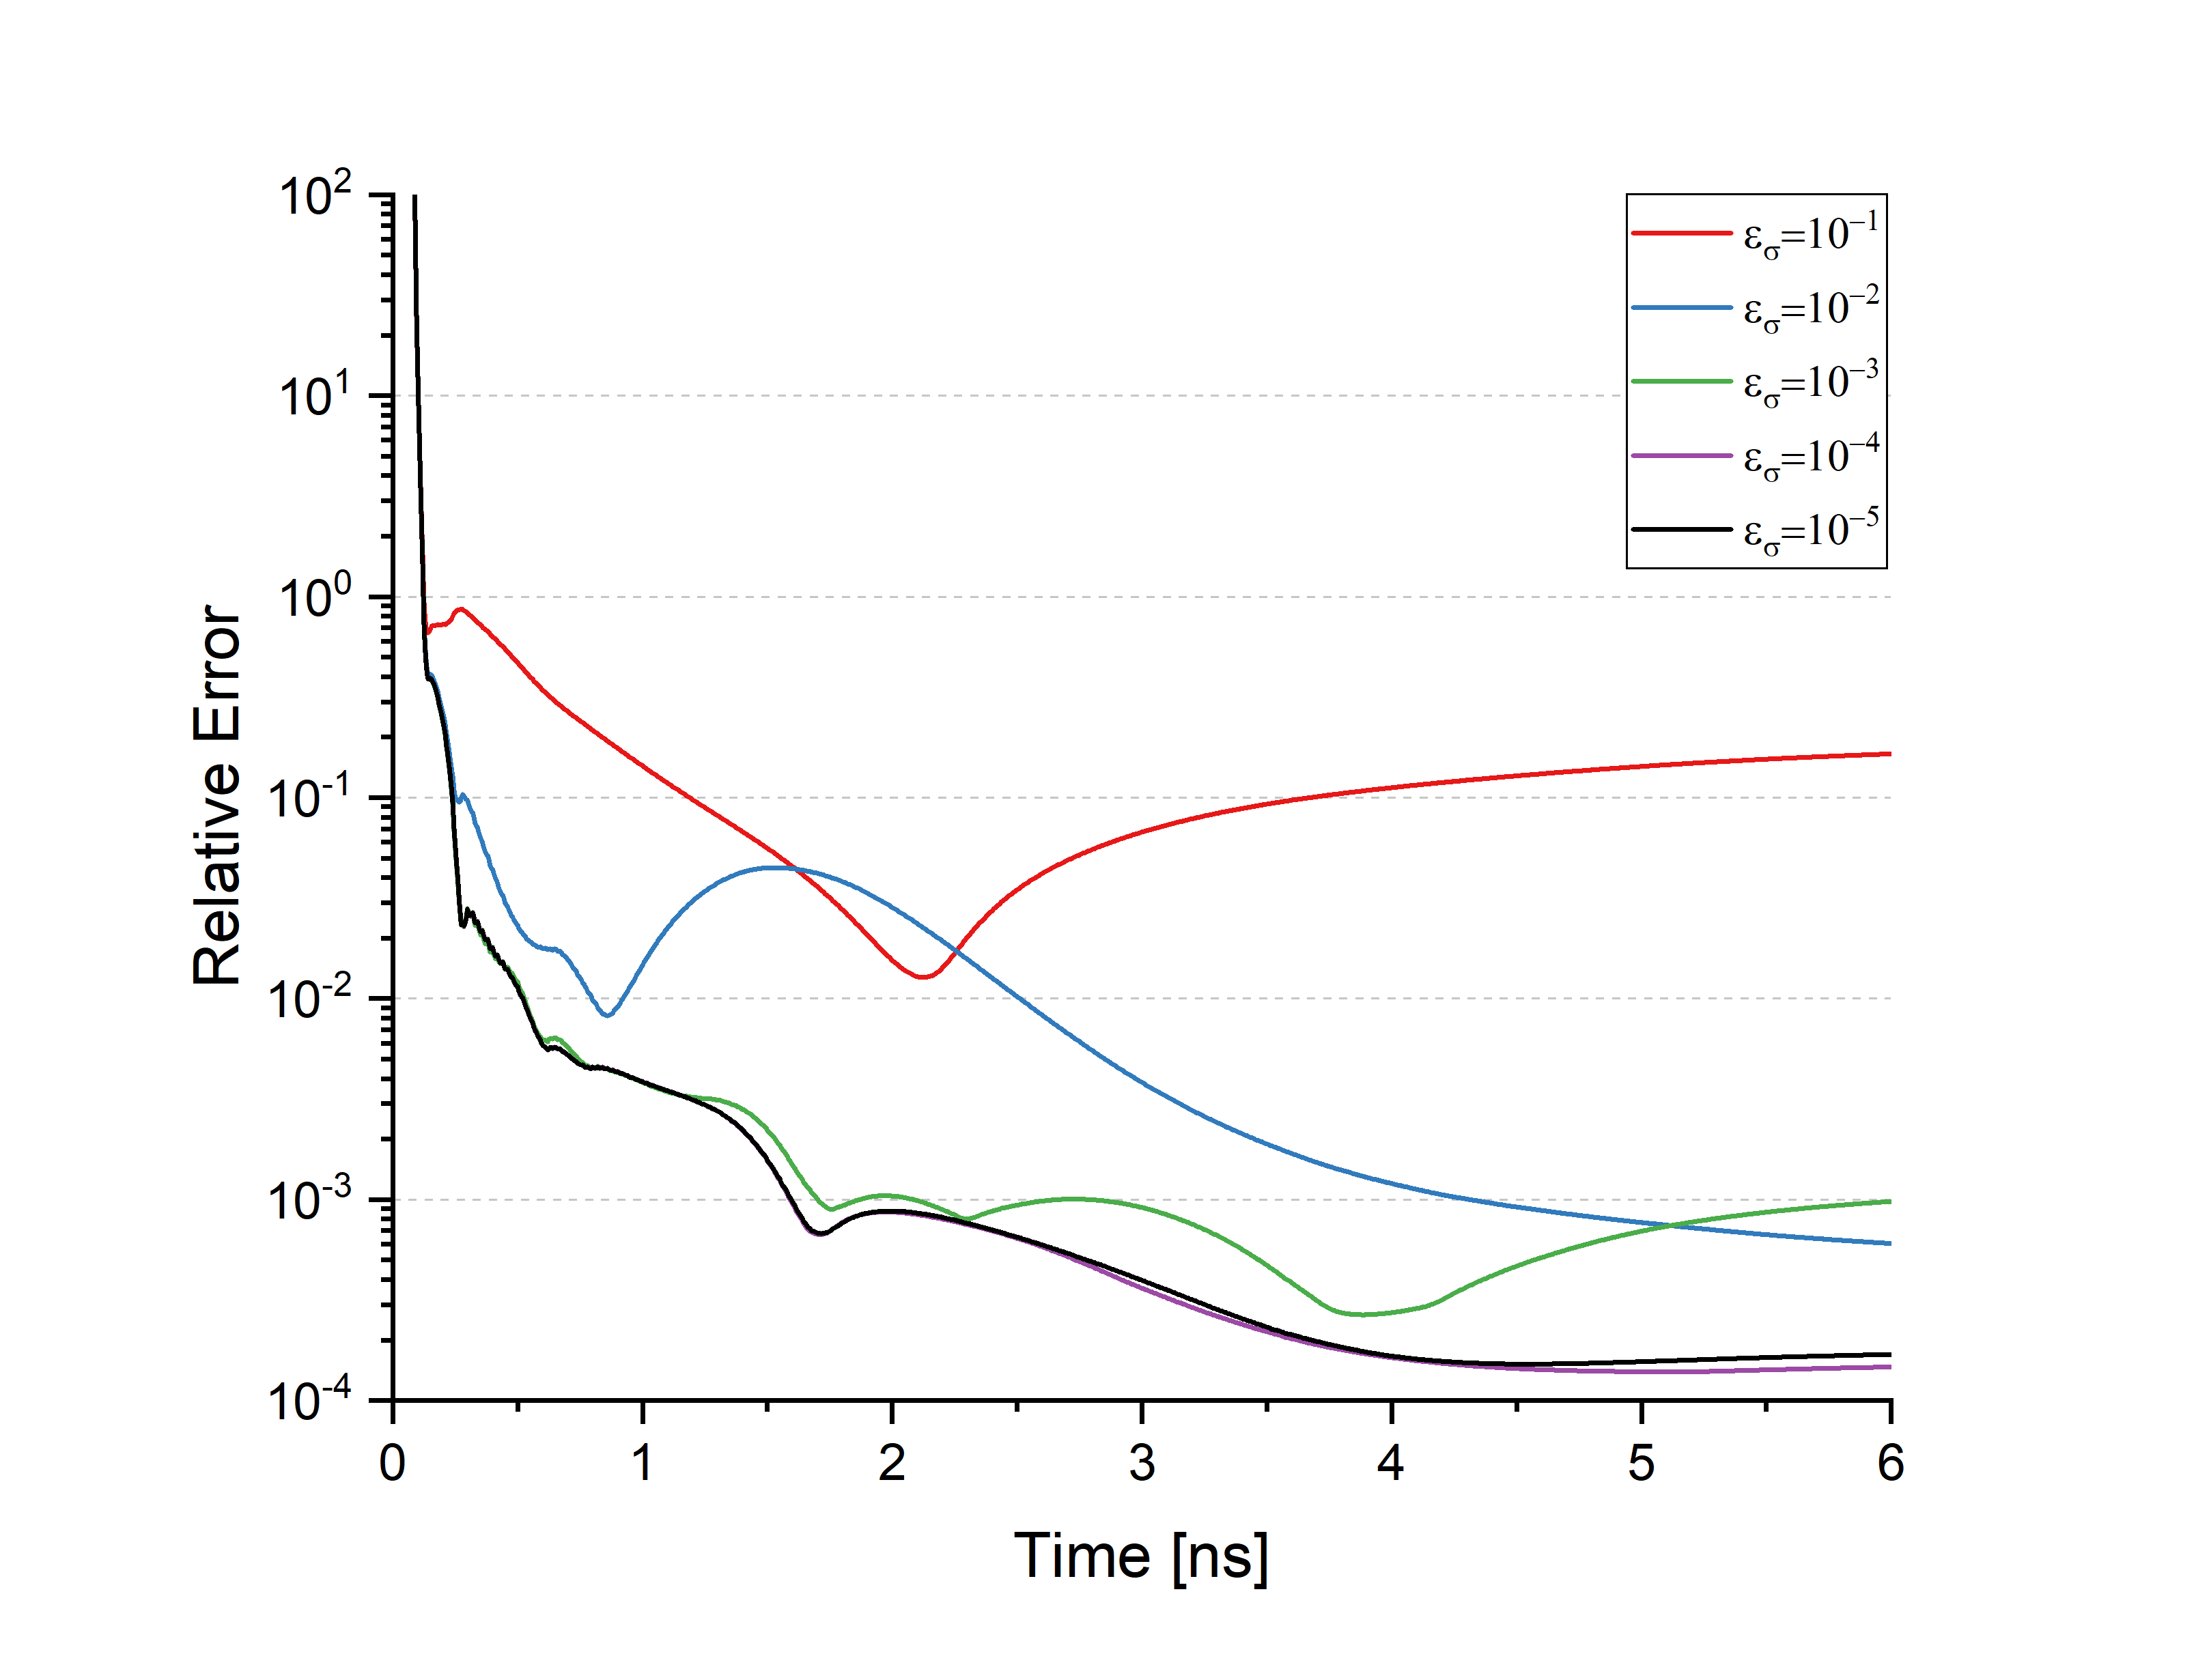
\includegraphics[width=0.475\textwidth]{GR_bc1000-t0005_qdf1000-t002_Eavg_grey_fg_bg.png}}\\
		\subfloat[Temperature relative error using reference $f_g$ and approximate $E_g$ \label{subfig:GR_bc1000-t0005_qdf1000-t002_Tavg_grey_Eg}]{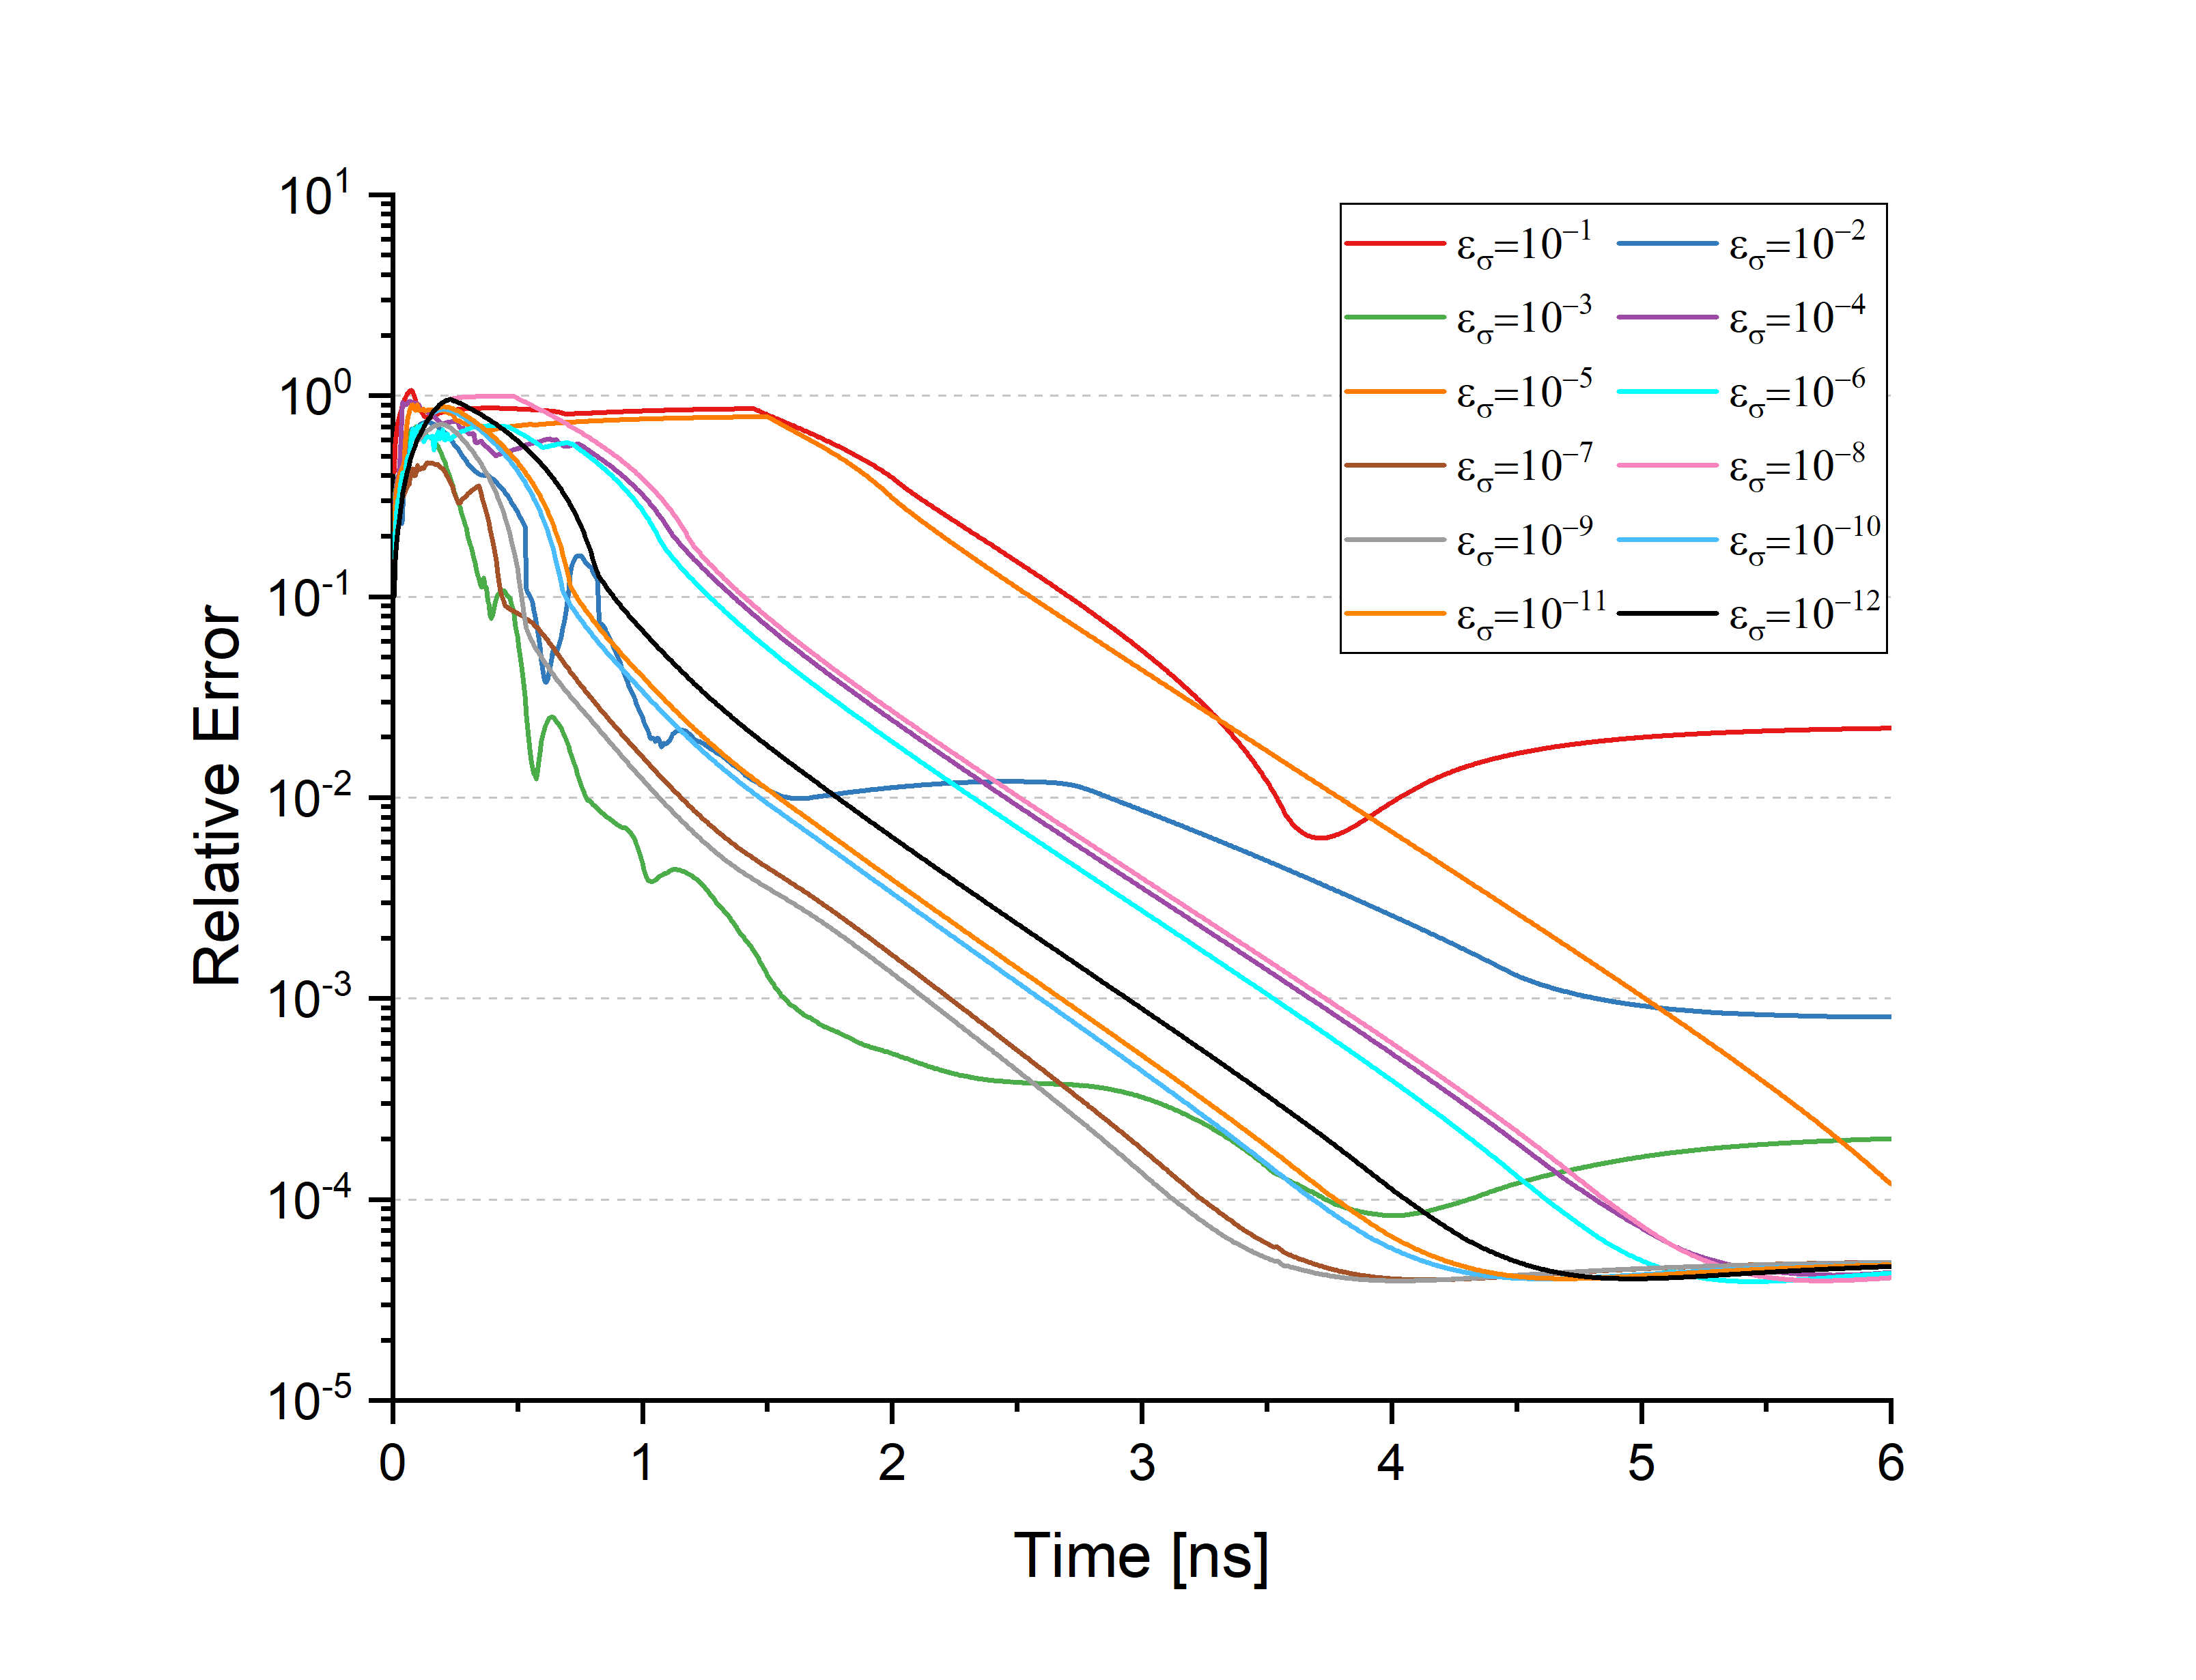
\includegraphics[width=0.475\textwidth]{GR_bc1000-t0005_qdf1000-t002_Tavg_grey_Eg_bg.png}}
		\subfloat[Energy density relative error using reference $f_g$ and approximate $E_g$ \label{subfig:GR_bc1000-t0005_qdf1000-t002_Eavg_grey_Eg}]{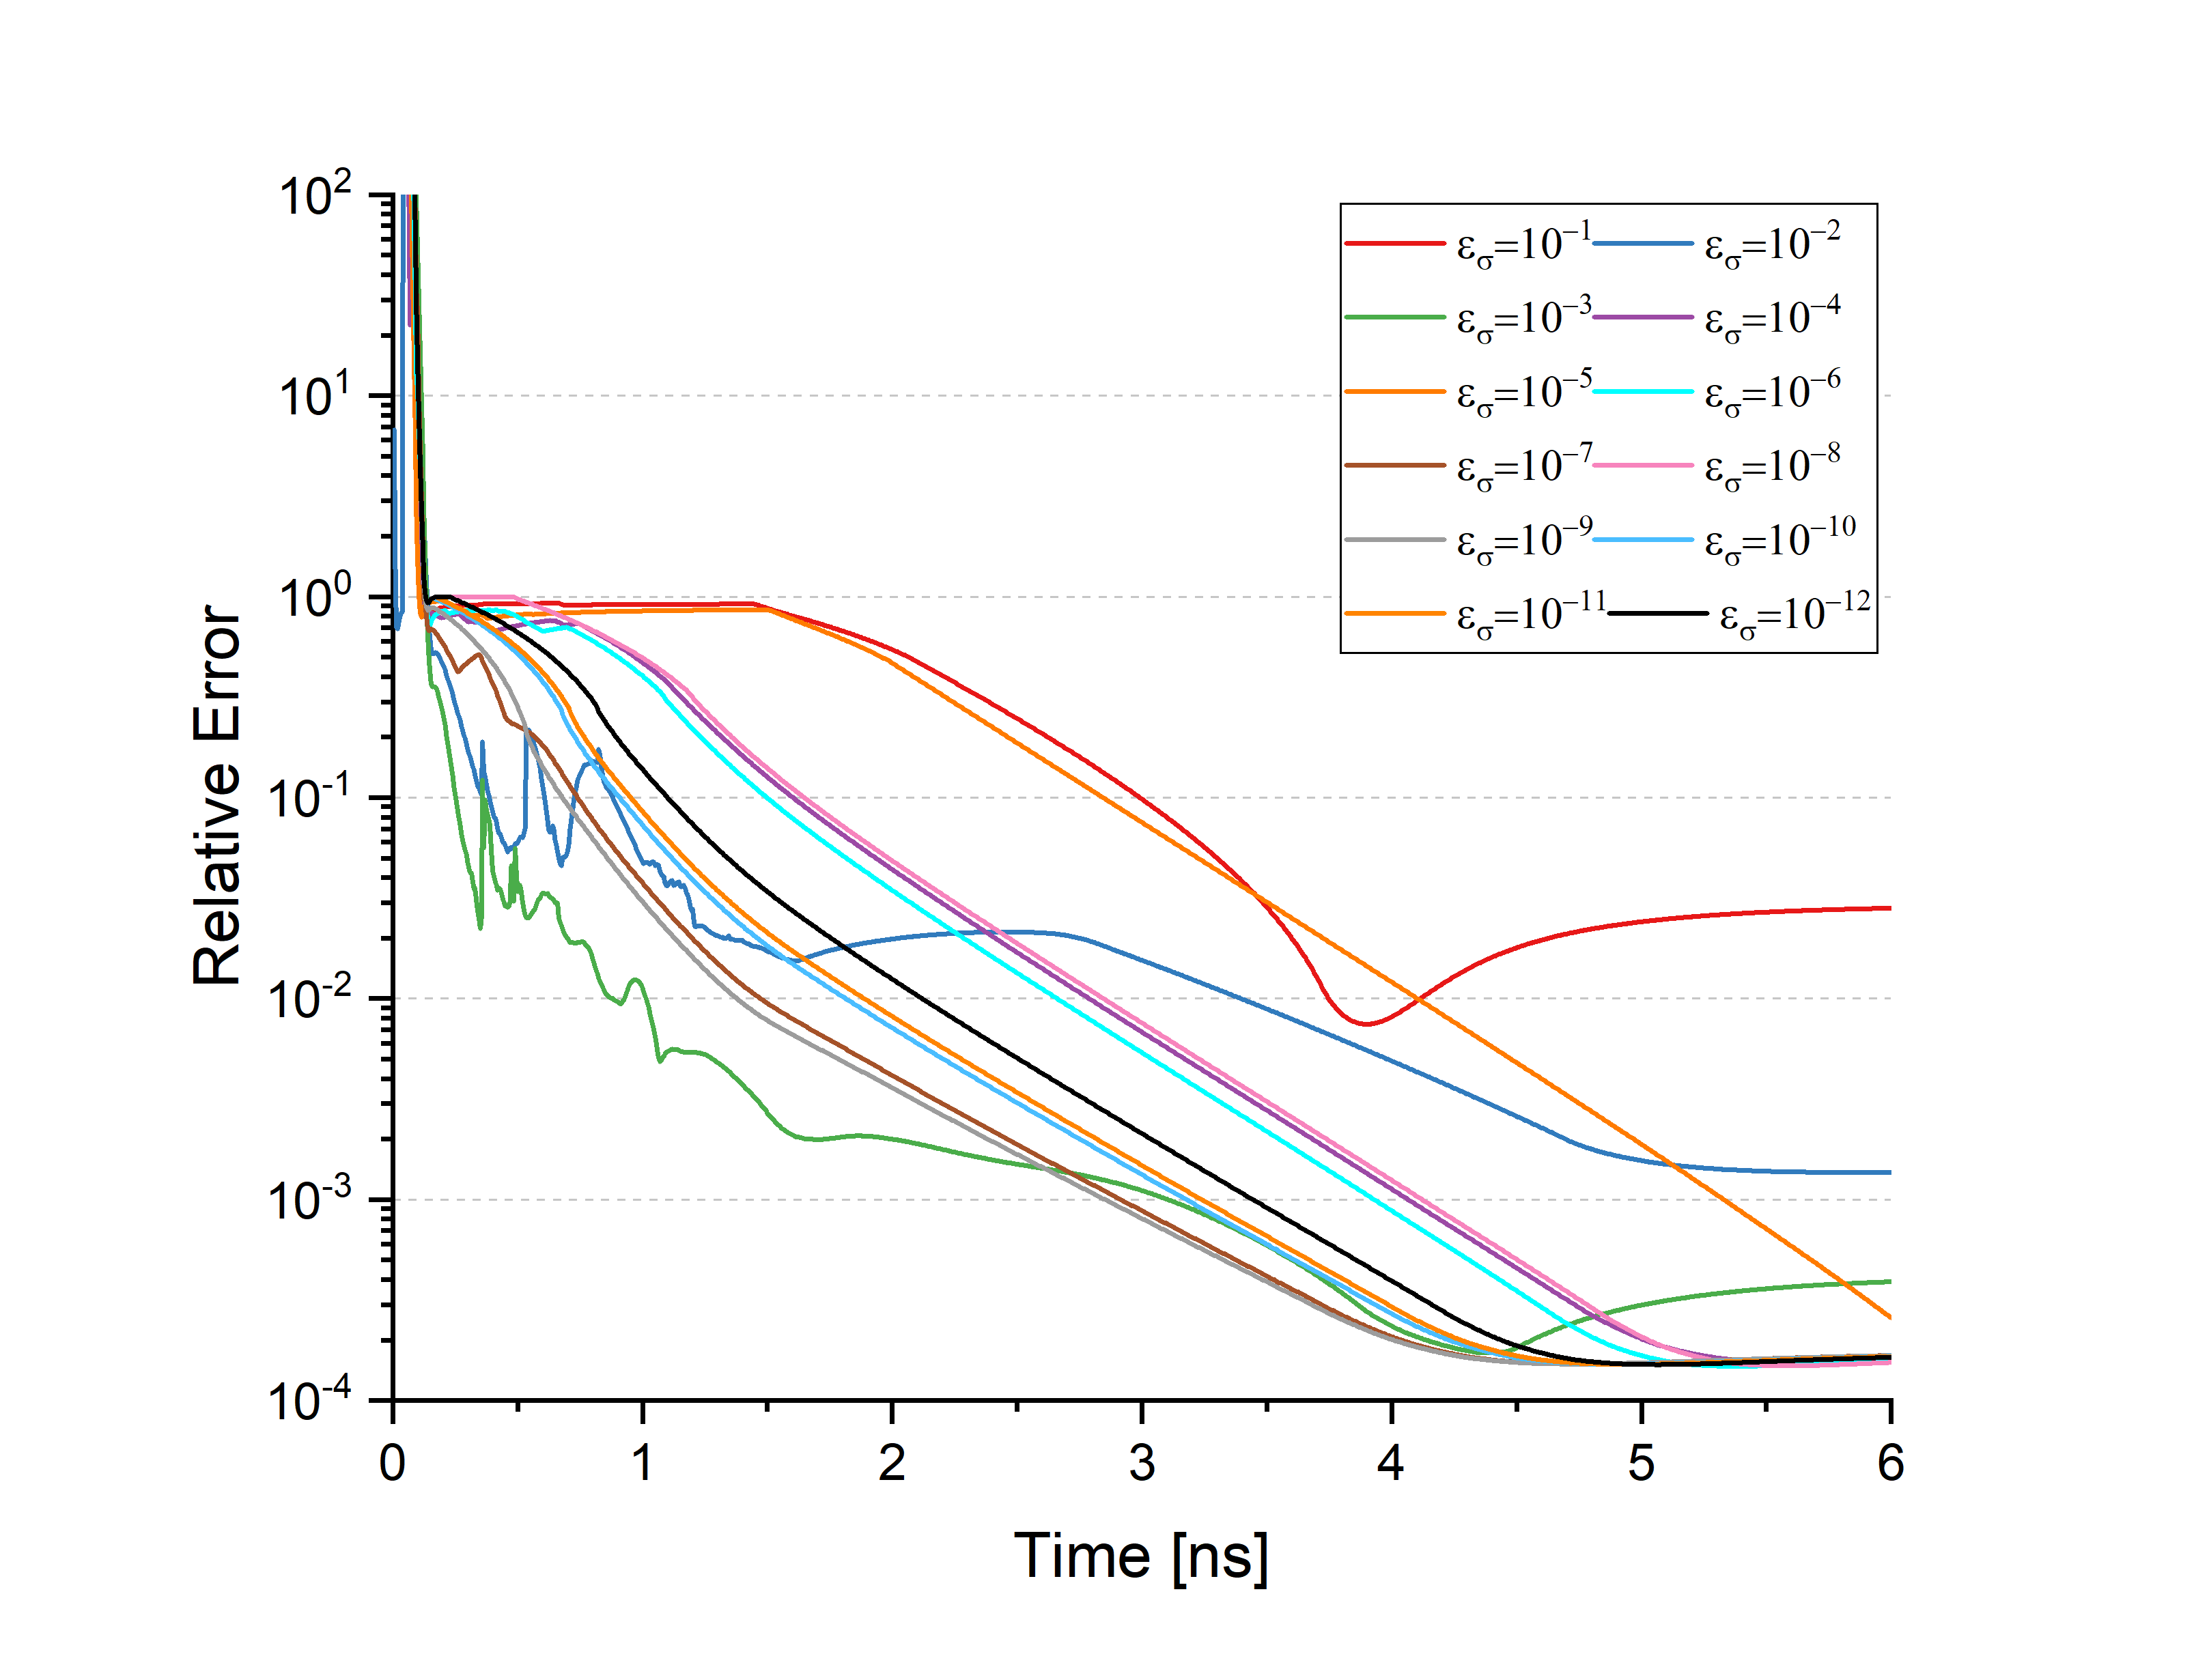
\includegraphics[width=0.475\textwidth]{GR_bc1000-t0005_qdf1000-t002_Eavg_grey_Eg_bg.png}}\\
		\subfloat[Temperature relative error using approximate \newline $f_g$ and approximate $E_g$ \label{subfig:GR_bc1000-t0005_qdf1000-t002_Tavg_grey_E-fg}]{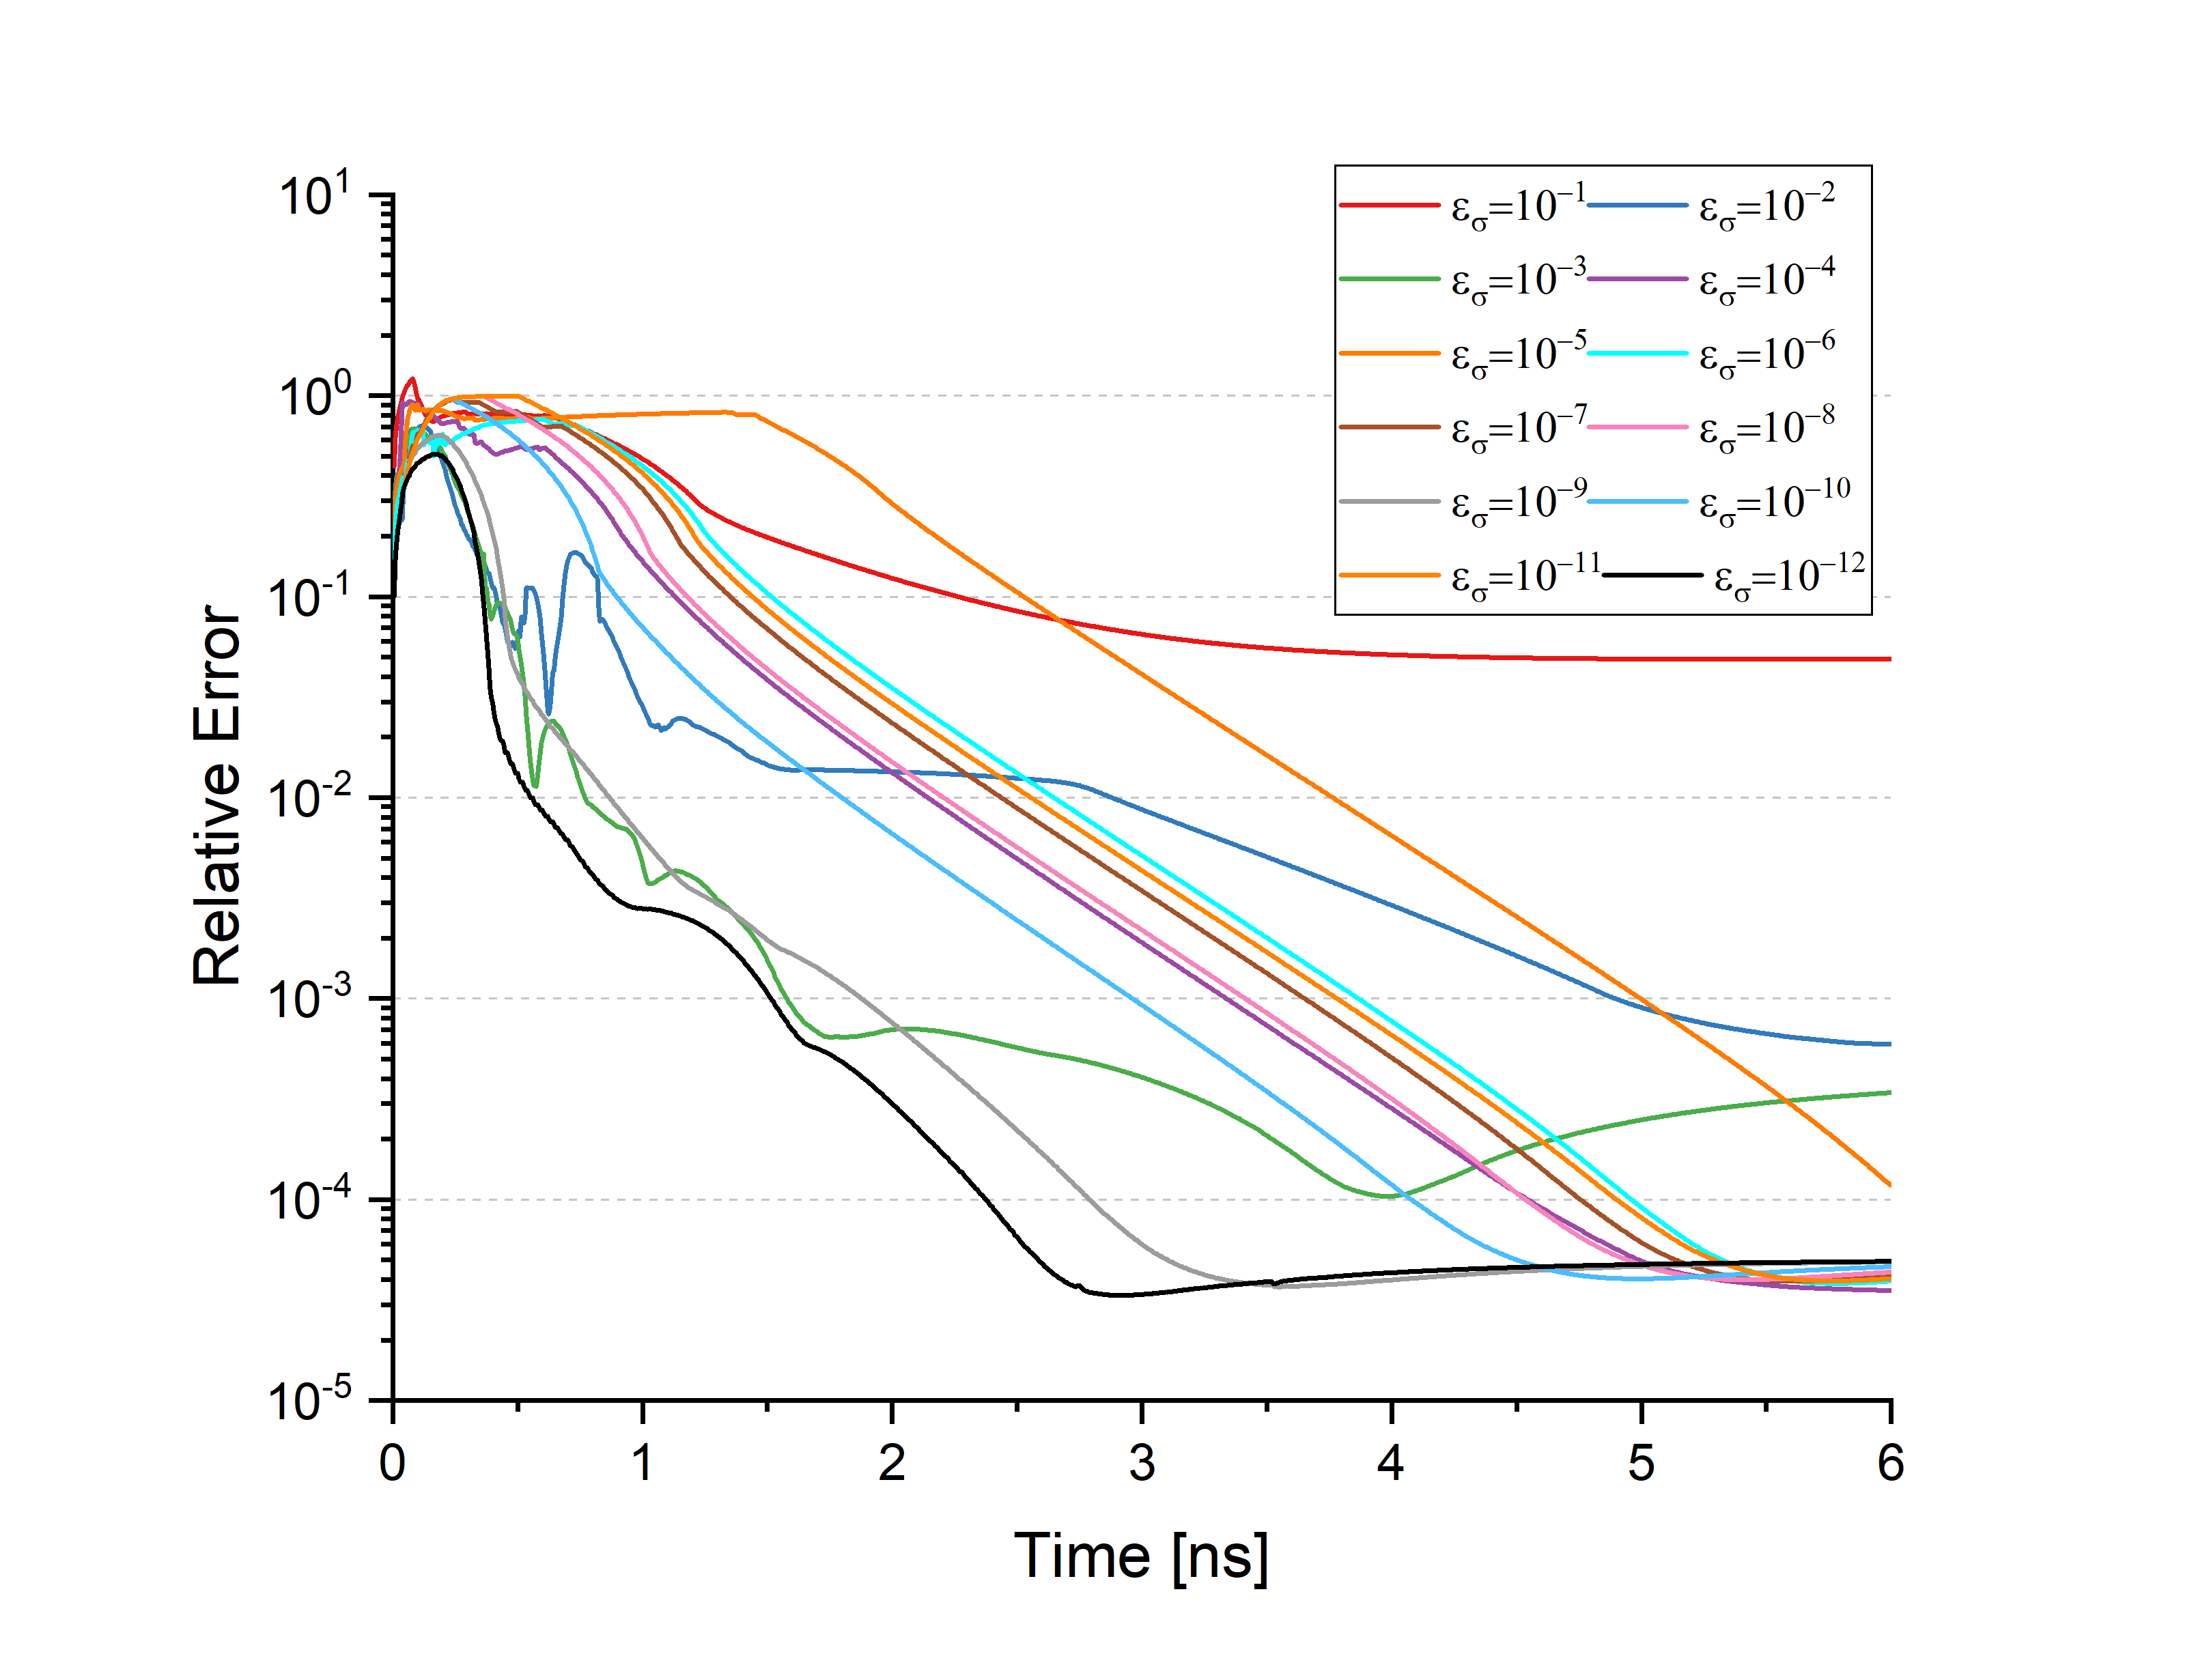
\includegraphics[width=0.475\textwidth]{GR_bc1000-t0005_qdf1000-t002_Tavg_grey_E-fg_bg}}
		\subfloat[Energy density relative error using approximate $f_g$ and approximate $E_g$ \label{subfig:GR_bc1000-t0005_qdf1000-t002_Eavg_grey_E-fg}]{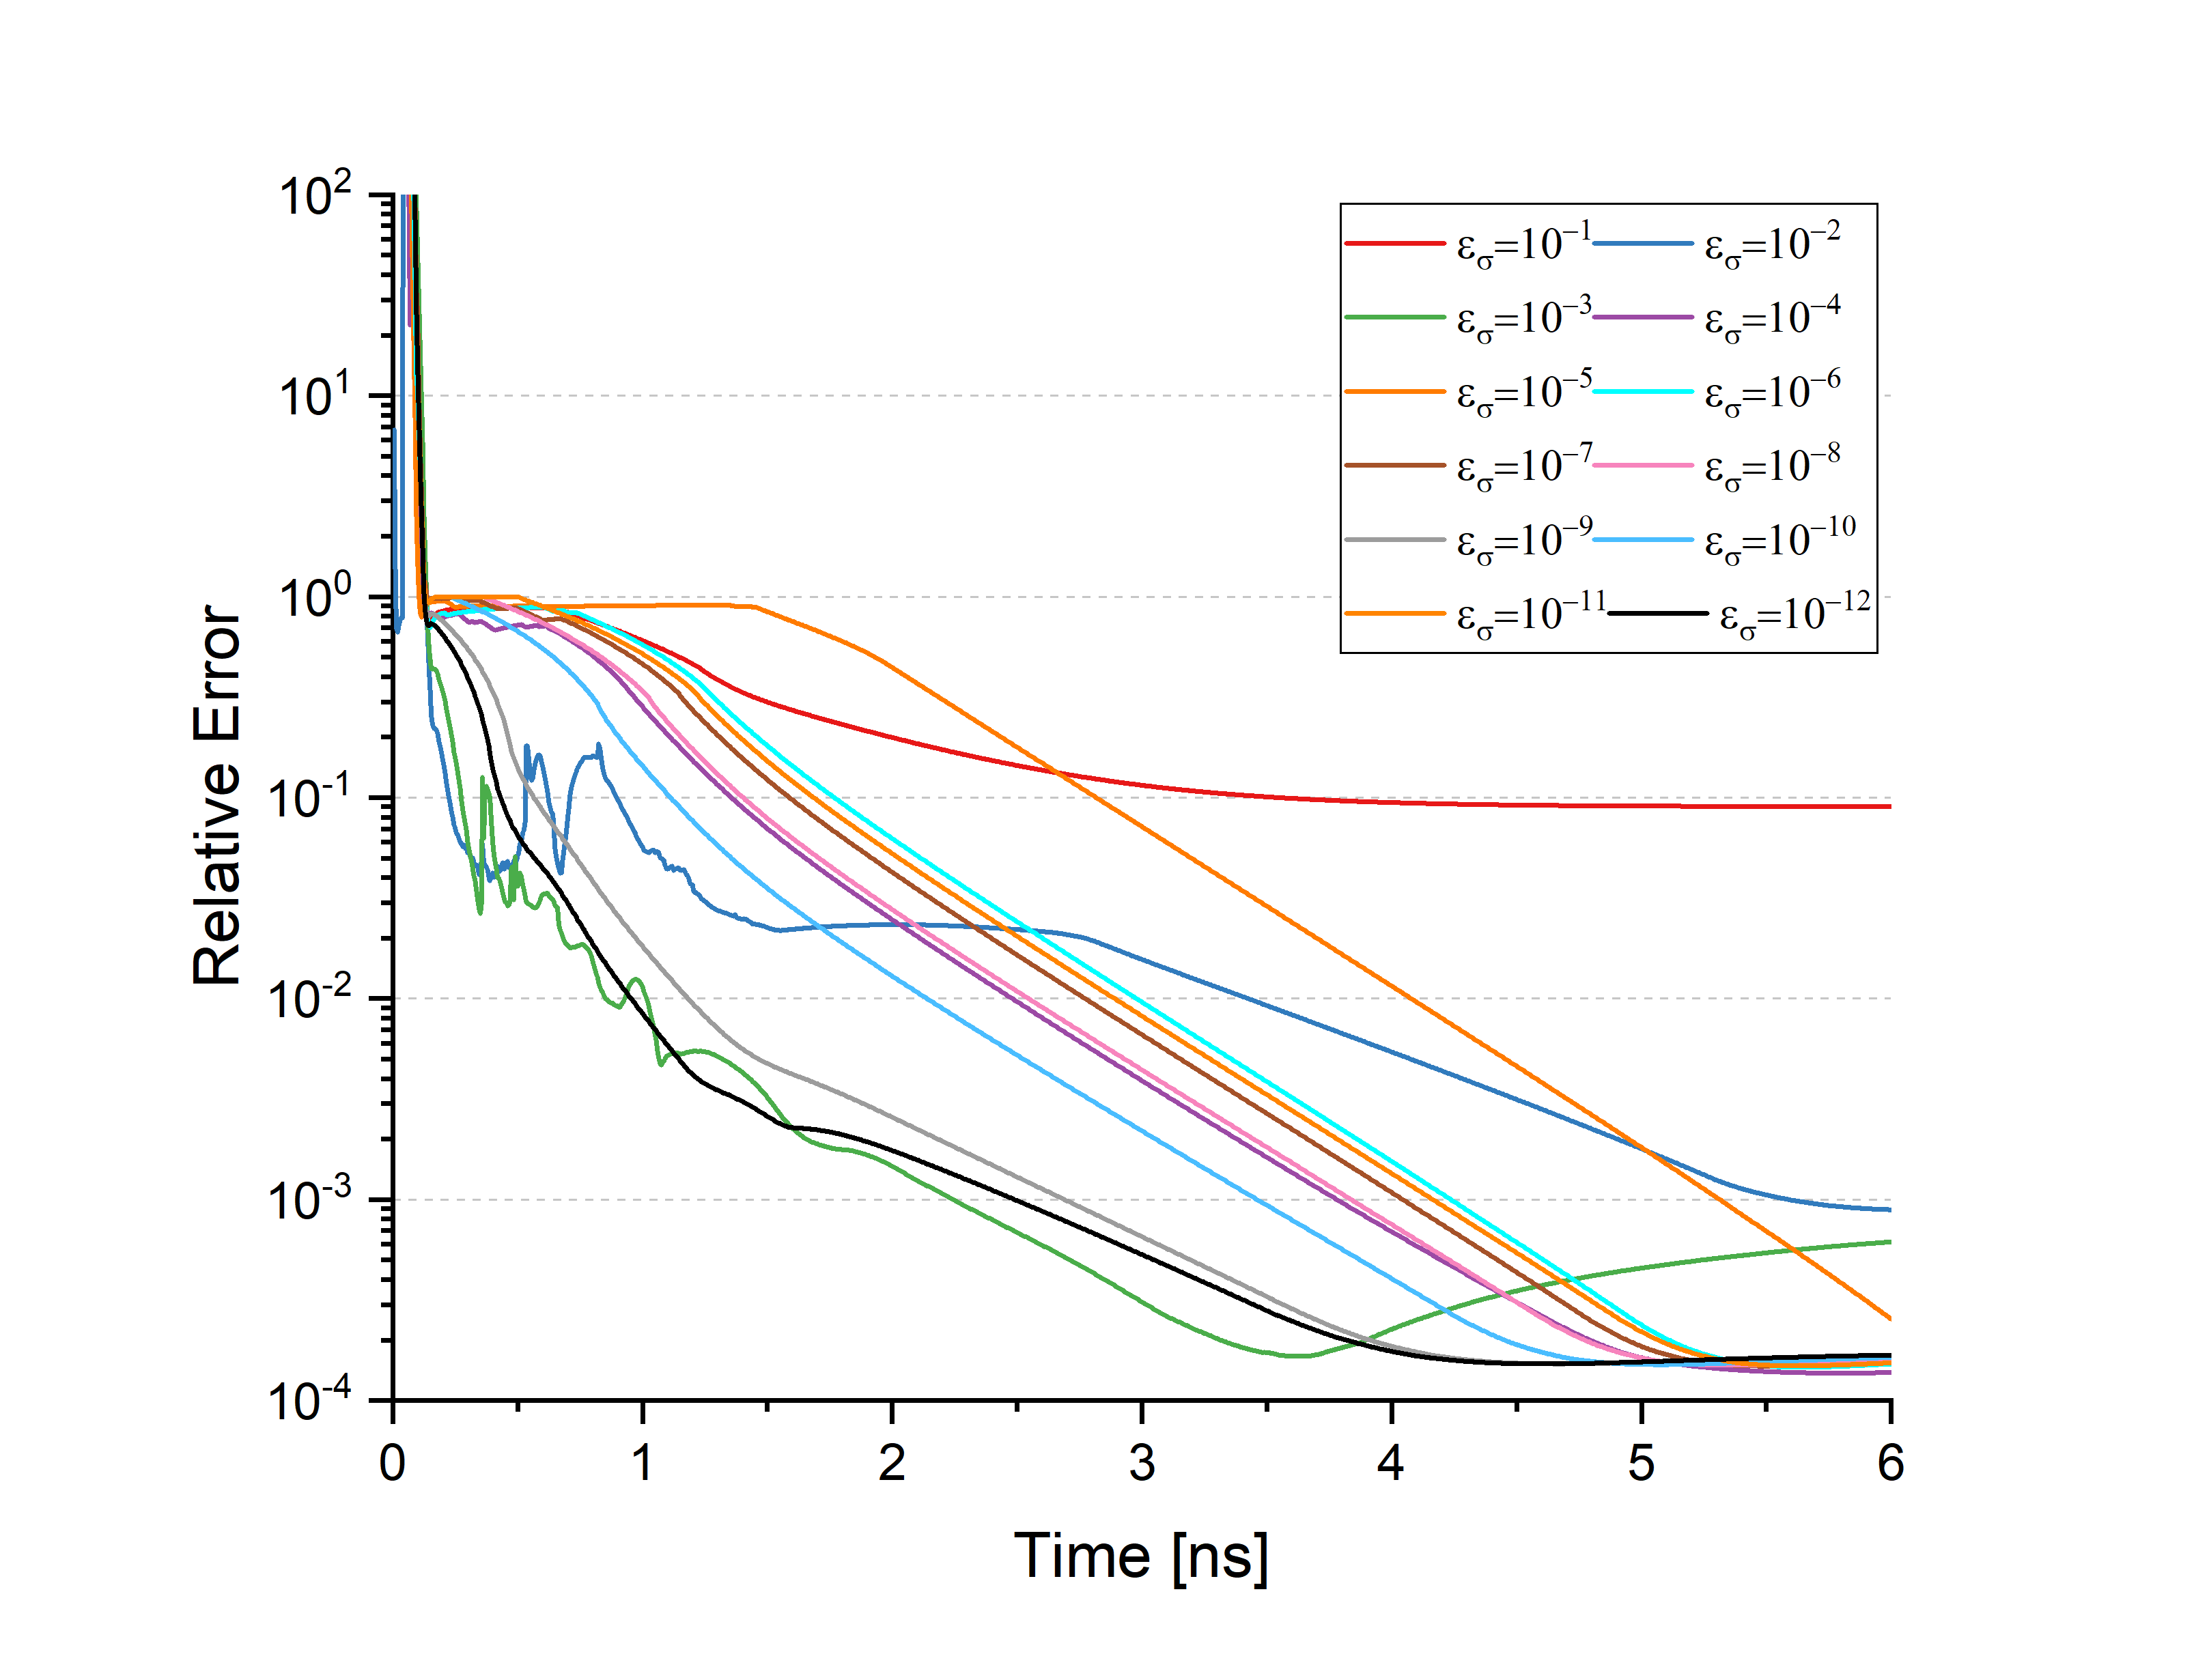
\includegraphics[width=0.475\textwidth]{GR_bc1000-t0005_qdf1000-t002_Eavg_grey_E-fg_bg}}
		\caption{\label{fig:errors_dt-0.005_grey}
			Relative error in the $L_1$-norm of GLOQD-POD solutions computed with $\Delta t\! =\! 5 \! \times \! 10^{-3}$~ns
			versus the reference TRT solution. Data for the GLOQD-POD model is generated with $\Delta t\! =\! 2 \! \times\!  10^{-2}$ ns. }
	\end{figure}

	\ind The GLOQD-POD ROM is also extended to develop a parameterized ROM for a class of TRT problems as done in Ch. \ref{chap-three} using QD factors and radiation energy densities estimated from a set of base cases. We consider a ROM parameterized with respect to the temperature $T_{in}$ of incoming radiation at the left boundary. A database of the group QD factors and radiation energy densities is formed for problems with two selected temperatures of incoming radiation  $T_{in}^{(1)}$ and $T_{in}^{(2)}$. The GLOQD-POD ROM solutions of TRT problems with incoming radiation at some given temperature are calculated using the group QD factors and radiation energy densities obtained by linear interpolation between values in the database. Results are presented for two parameterized ROMs. One model uses $T_{in}^{(1)}~=~1$~KeV and $T_{in}^{(2)}=0.98$ KeV. The second one is formed with  $T_{in}^{(1)}=1$ KeV and $T_{in}^{(2)}=0.96$ KeV. The data is generated for $\Delta t = 2\times10^{-2}$ ns. Fig. \ref{fig:errors_bc_T=990_grey} shows the relative error in $L_1$-norm in the solution for $T_{in}=0.99$ KeV computed by means of first parametrized GLOQD-POD ROM with various values of $\varepsilon_{\sigma}$. Fig. \ref{fig:errors_bc_T=980_grey} presents the relative error of the GLOQD-POD ROM solution  for $T_{in}= 0.98$ KeV obtained from the second model that is parametrized with a larger interval of  $[T_{in}^{(1)},T_{in}^{(2)}]$. The reference MLQD solution is computed for each value of $T_{in}$ to obtain relative errors. The error for most cases saturated at $10^{-5} \leq \varepsilon_\sigma \leq 10^{-9}$ and so smaller $\varepsilon_\sigma$ are not shown. The cases which used reduced rank QD factors and exact energy densities had very similar errors to the cases shown for the MLOQD-POD ROM for the same parameterization in $T_{in}$. The saturated error for using only reduced rank QD factors, only energy densities or both in reduced rank form is similar in magnitude and shape. The saturated error for all cases increases as the interval of  $[T_{in}^{(1)},T_{in}^{(2)}]$ is increased, seeing roughly a 5 times increase between $T_{in}= 0.99$ KeV and $T_{in}= 0.98$ KeV. The effect causing large $\varepsilon_\sigma$ to be more accurate than small $\varepsilon_\sigma$ is not significantly present for either of these ROMs.
	
	%=================================================================================
	% BOUNDARY CONDITION DATABASE ERRORS PLOT
	\begin{figure}[ht!]
		\centering
		\subfloat[reduced rank QD factor temperature error \label{subfig:GR_bc990-t002_qdf1000-980-t002_Tavg_grey_fg}]{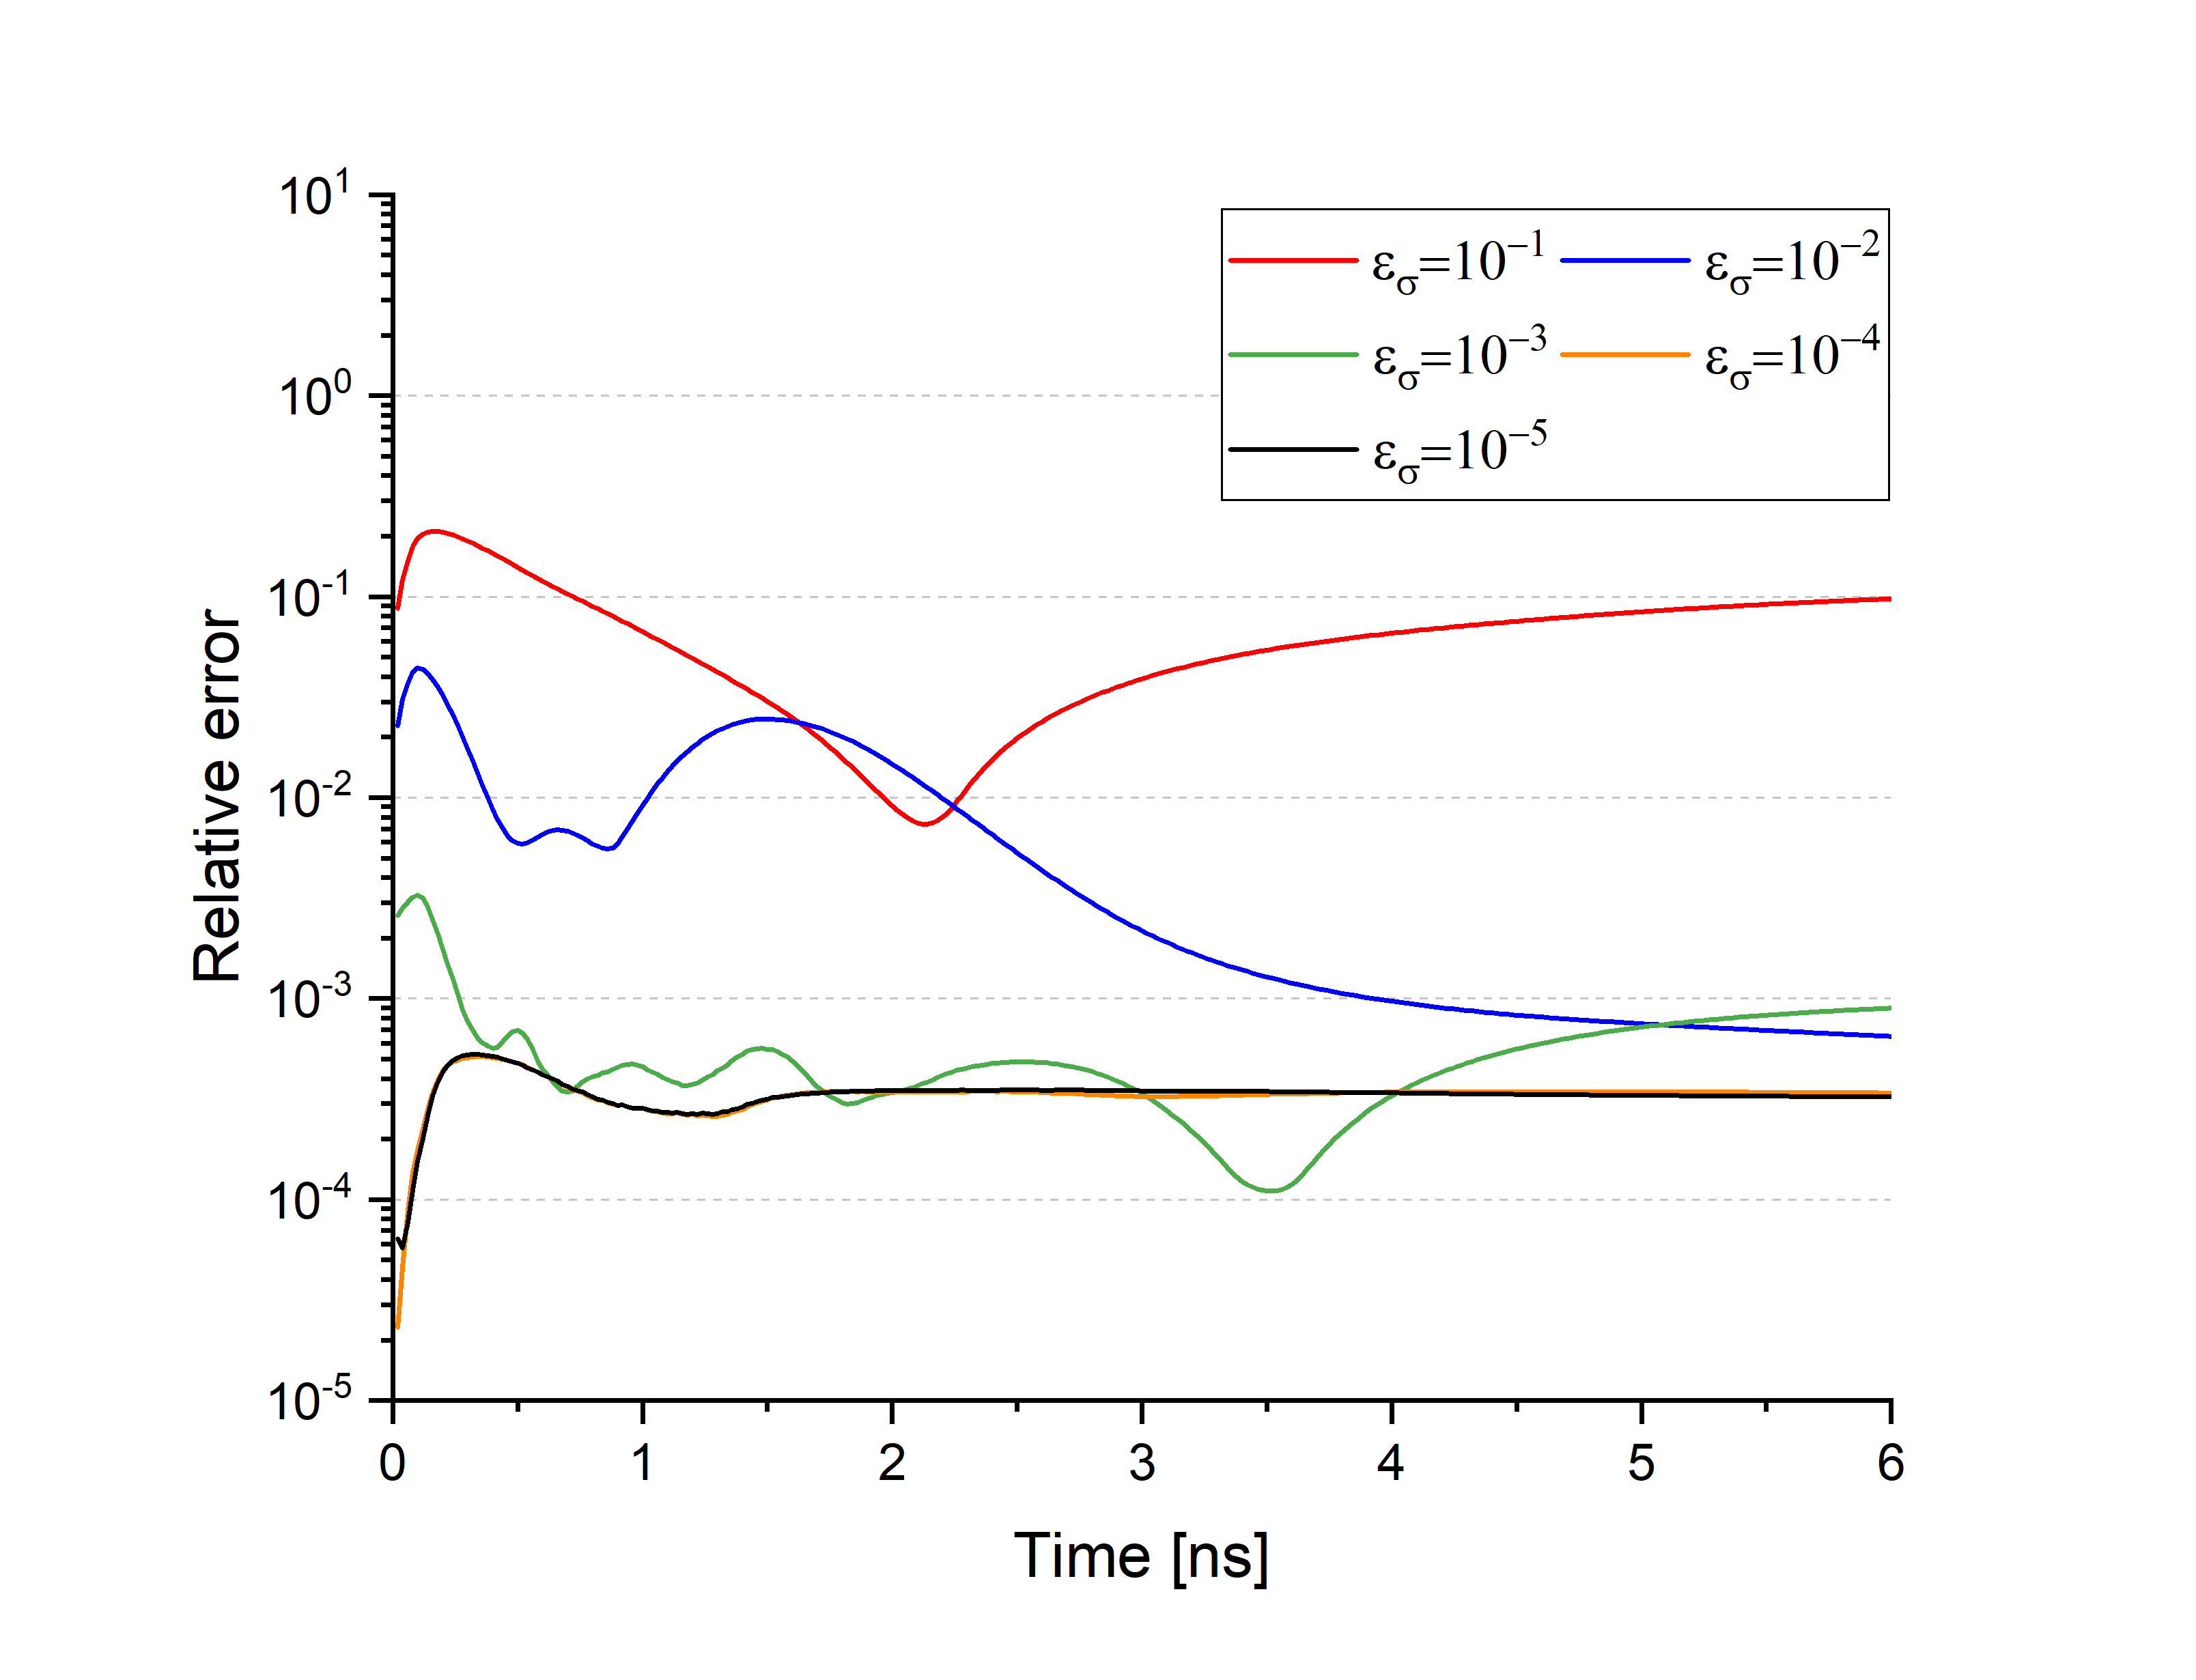
\includegraphics[width=0.475\textwidth]{GR_bc990-t002_qdf1000-980-t002_Tavg_grey_fg_bg.png}}
		\subfloat[reduced rank QD factor total energy density error \label{subfig:GR_bc990-t002_qdf1000-980-t002_Eavg_grey_fg}]{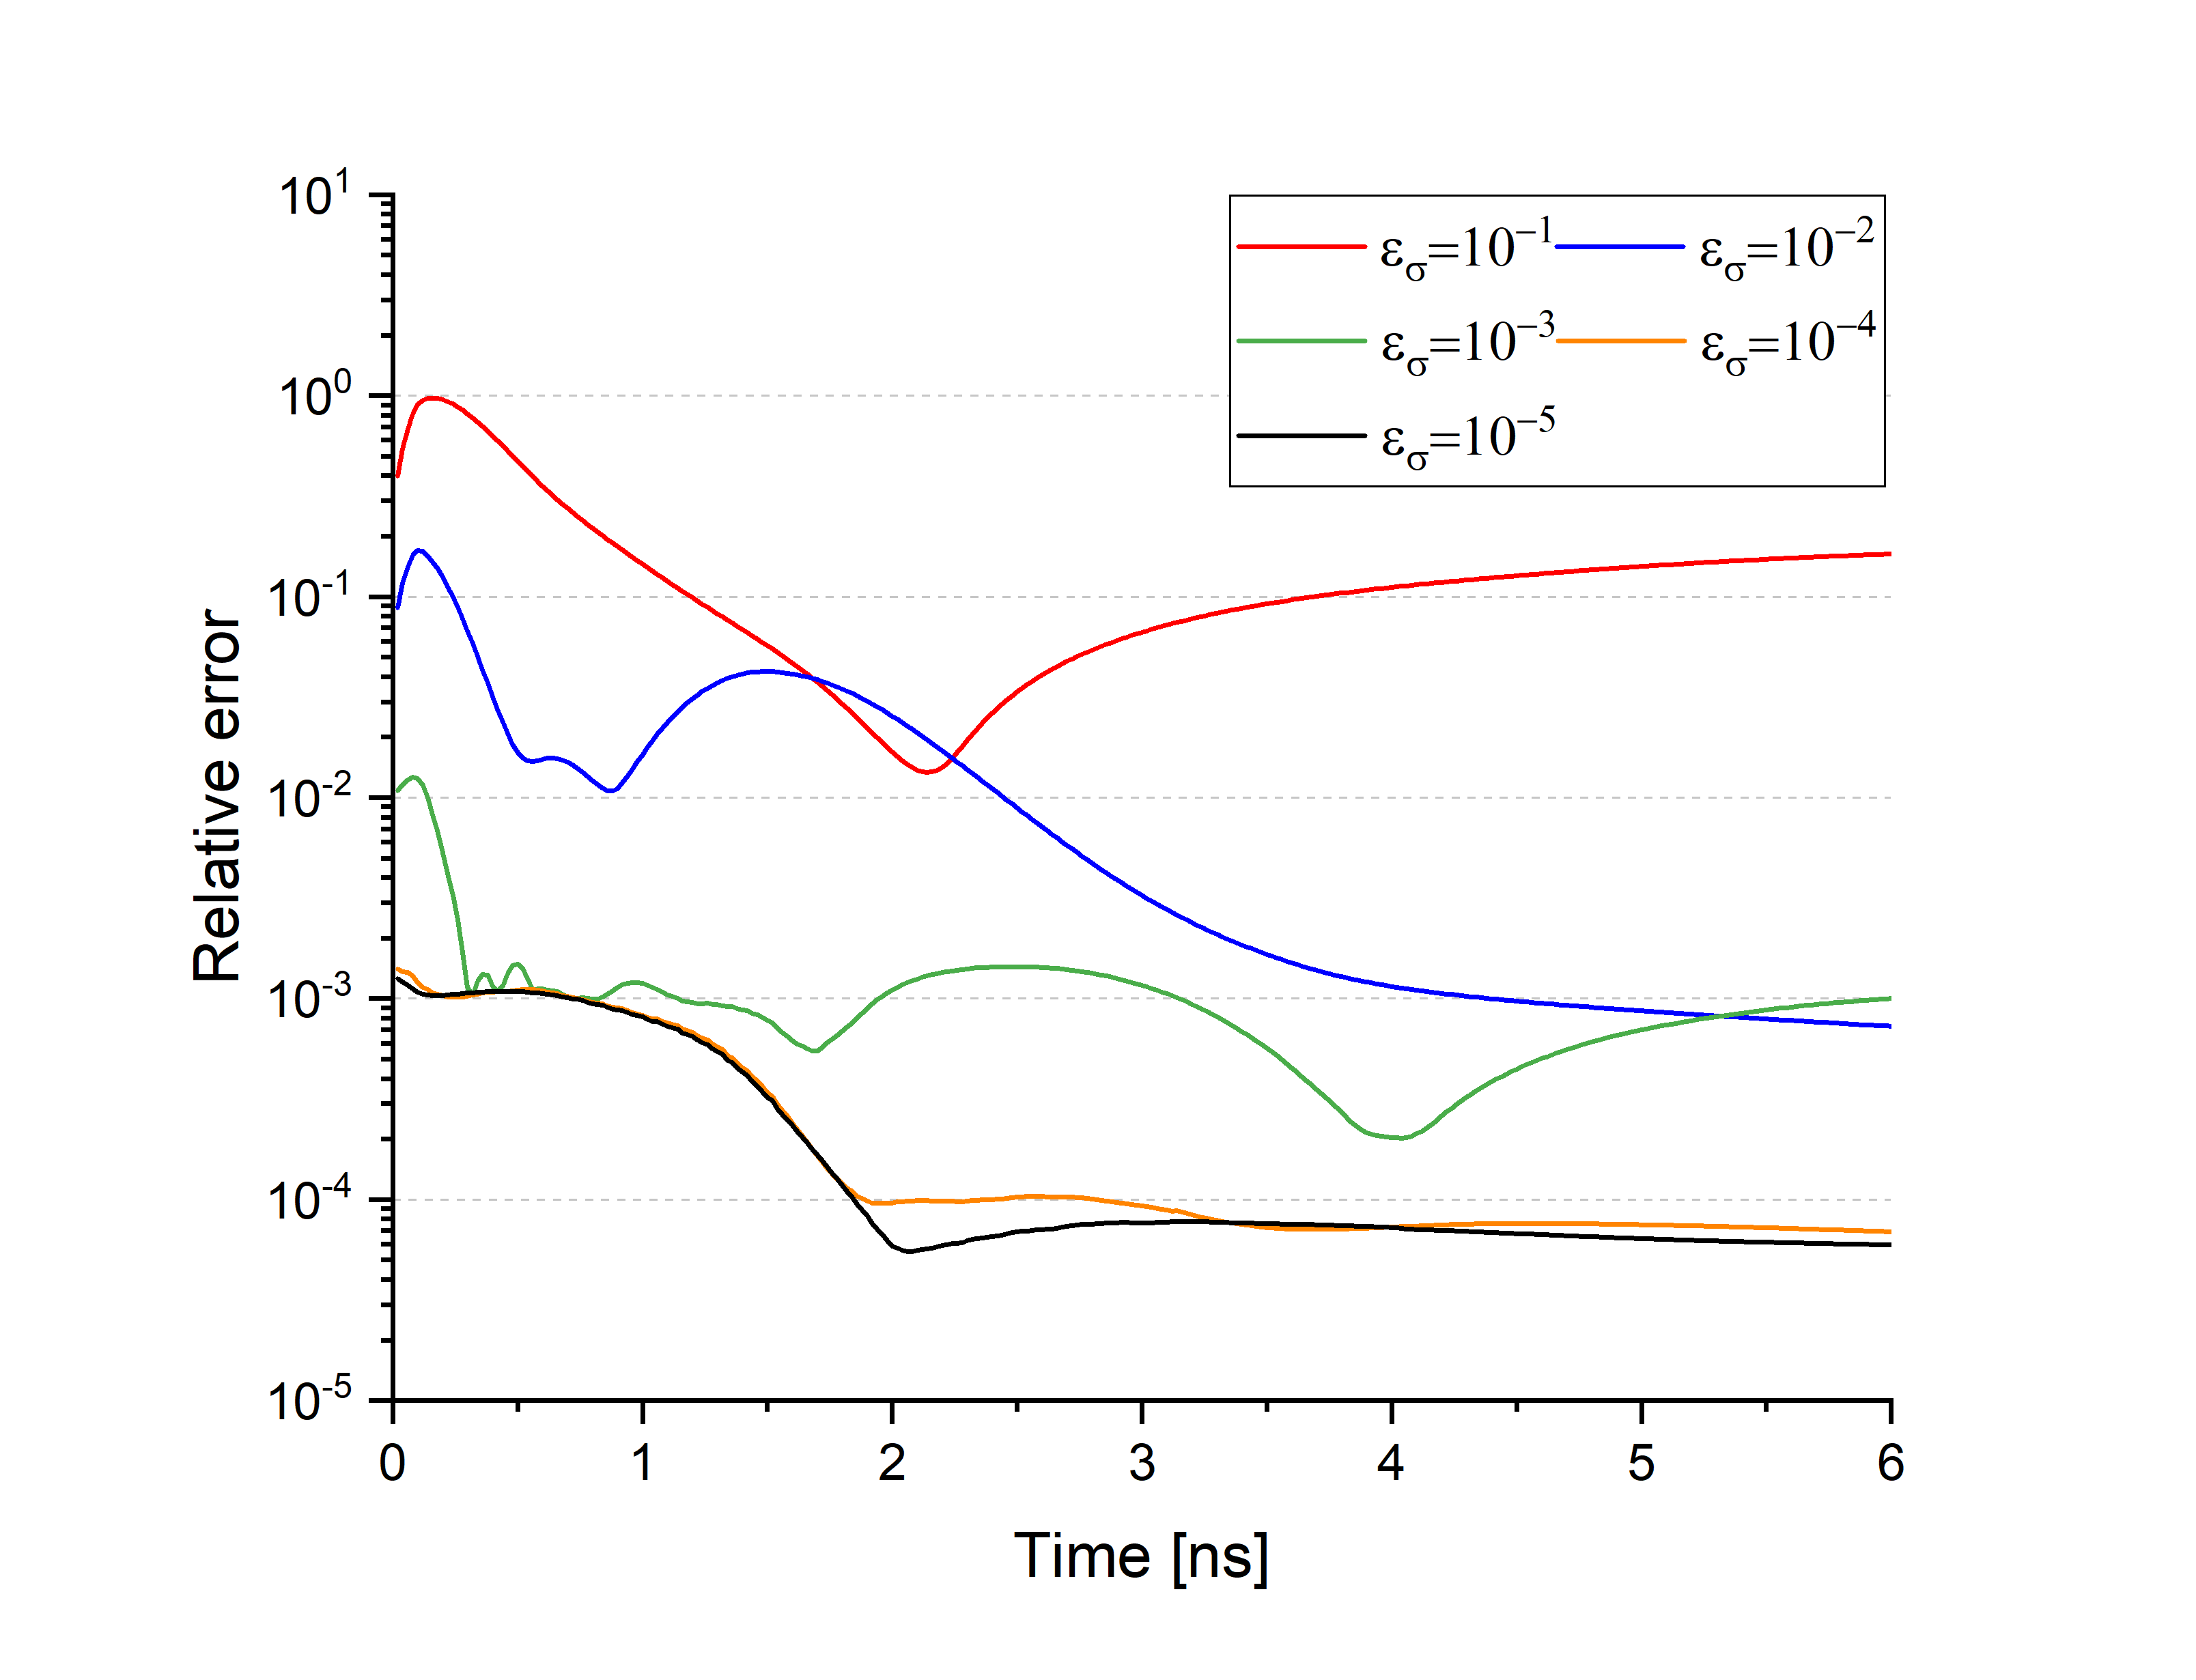
\includegraphics[width=0.475\textwidth]{GR_bc990-t002_qdf1000-980-t002_Eavg_grey_fg_bg.png}}\\
		\subfloat[reduced rank energy density temperature error \label{subfig:GR_bc990-t002_qdf1000-980-t002_Tavg_grey_Eg}]{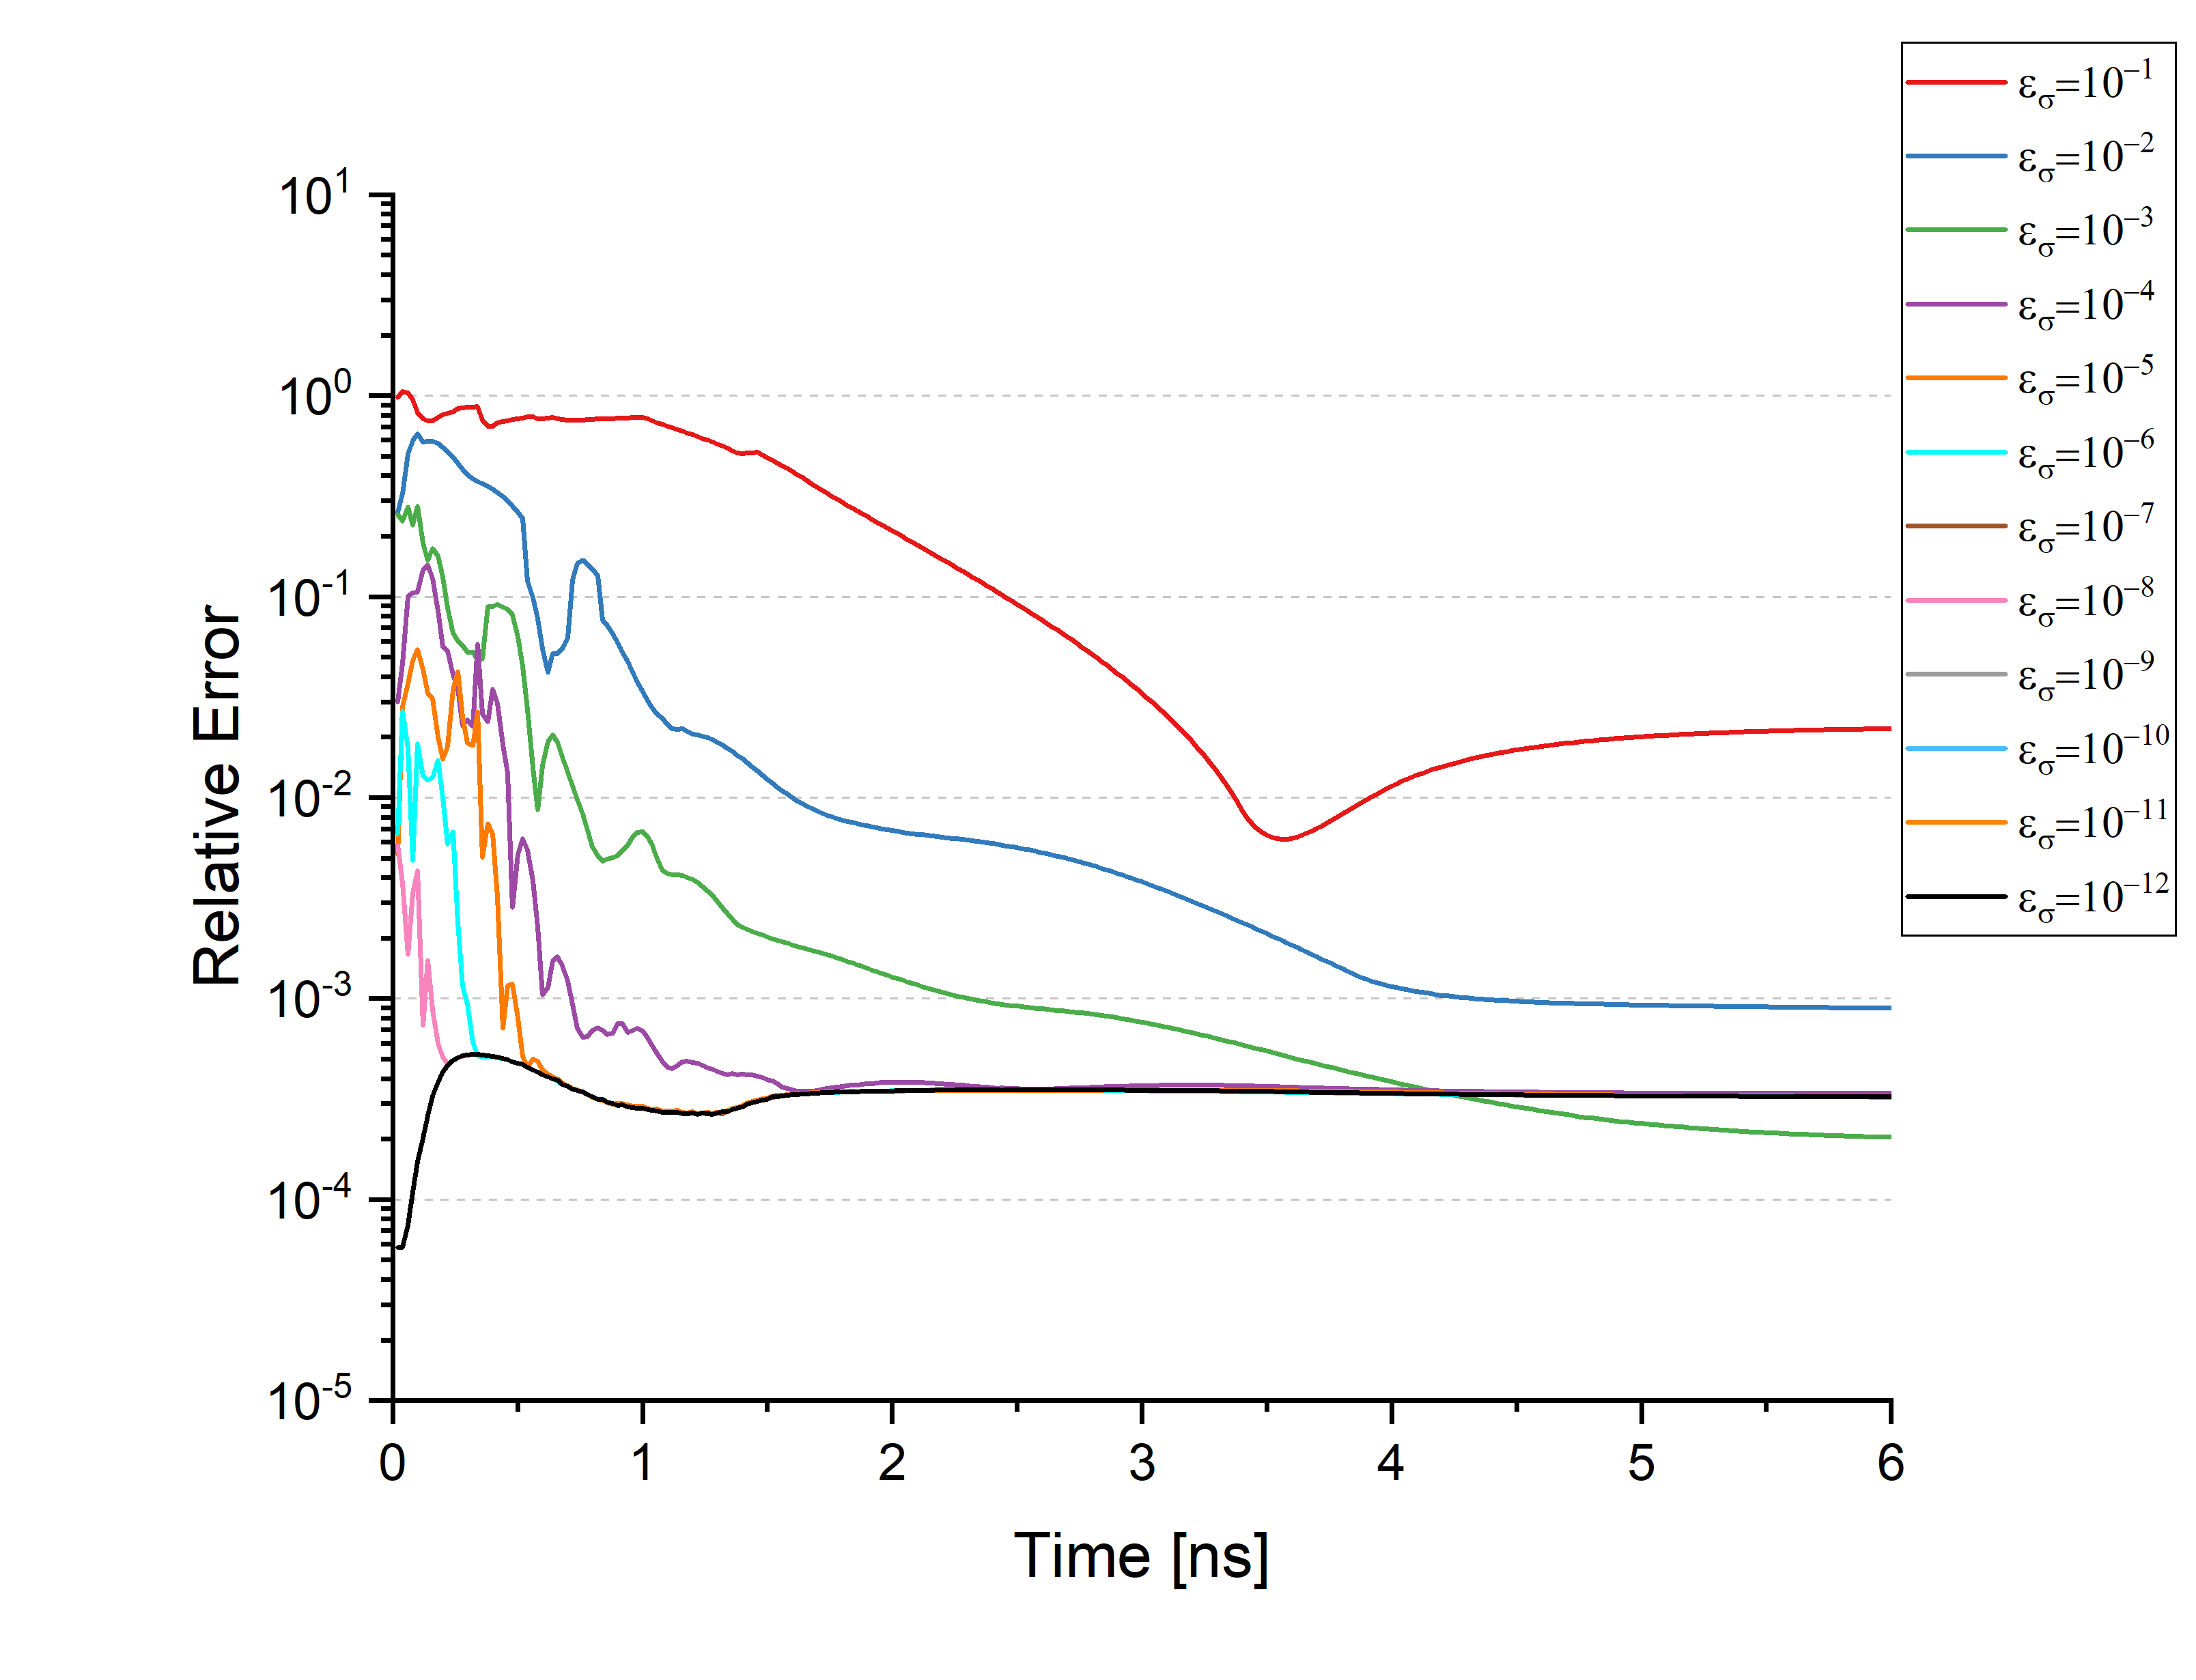
\includegraphics[width=0.475\textwidth]{GR_bc990-t002_qdf1000-980-t002_Tavg_grey_Eg_bg.png}}
		\subfloat[reduced rank energy density total energy density error \label{subfig:GR_bc990-t002_qdf1000-980-t002_Eavg_grey_Eg}]{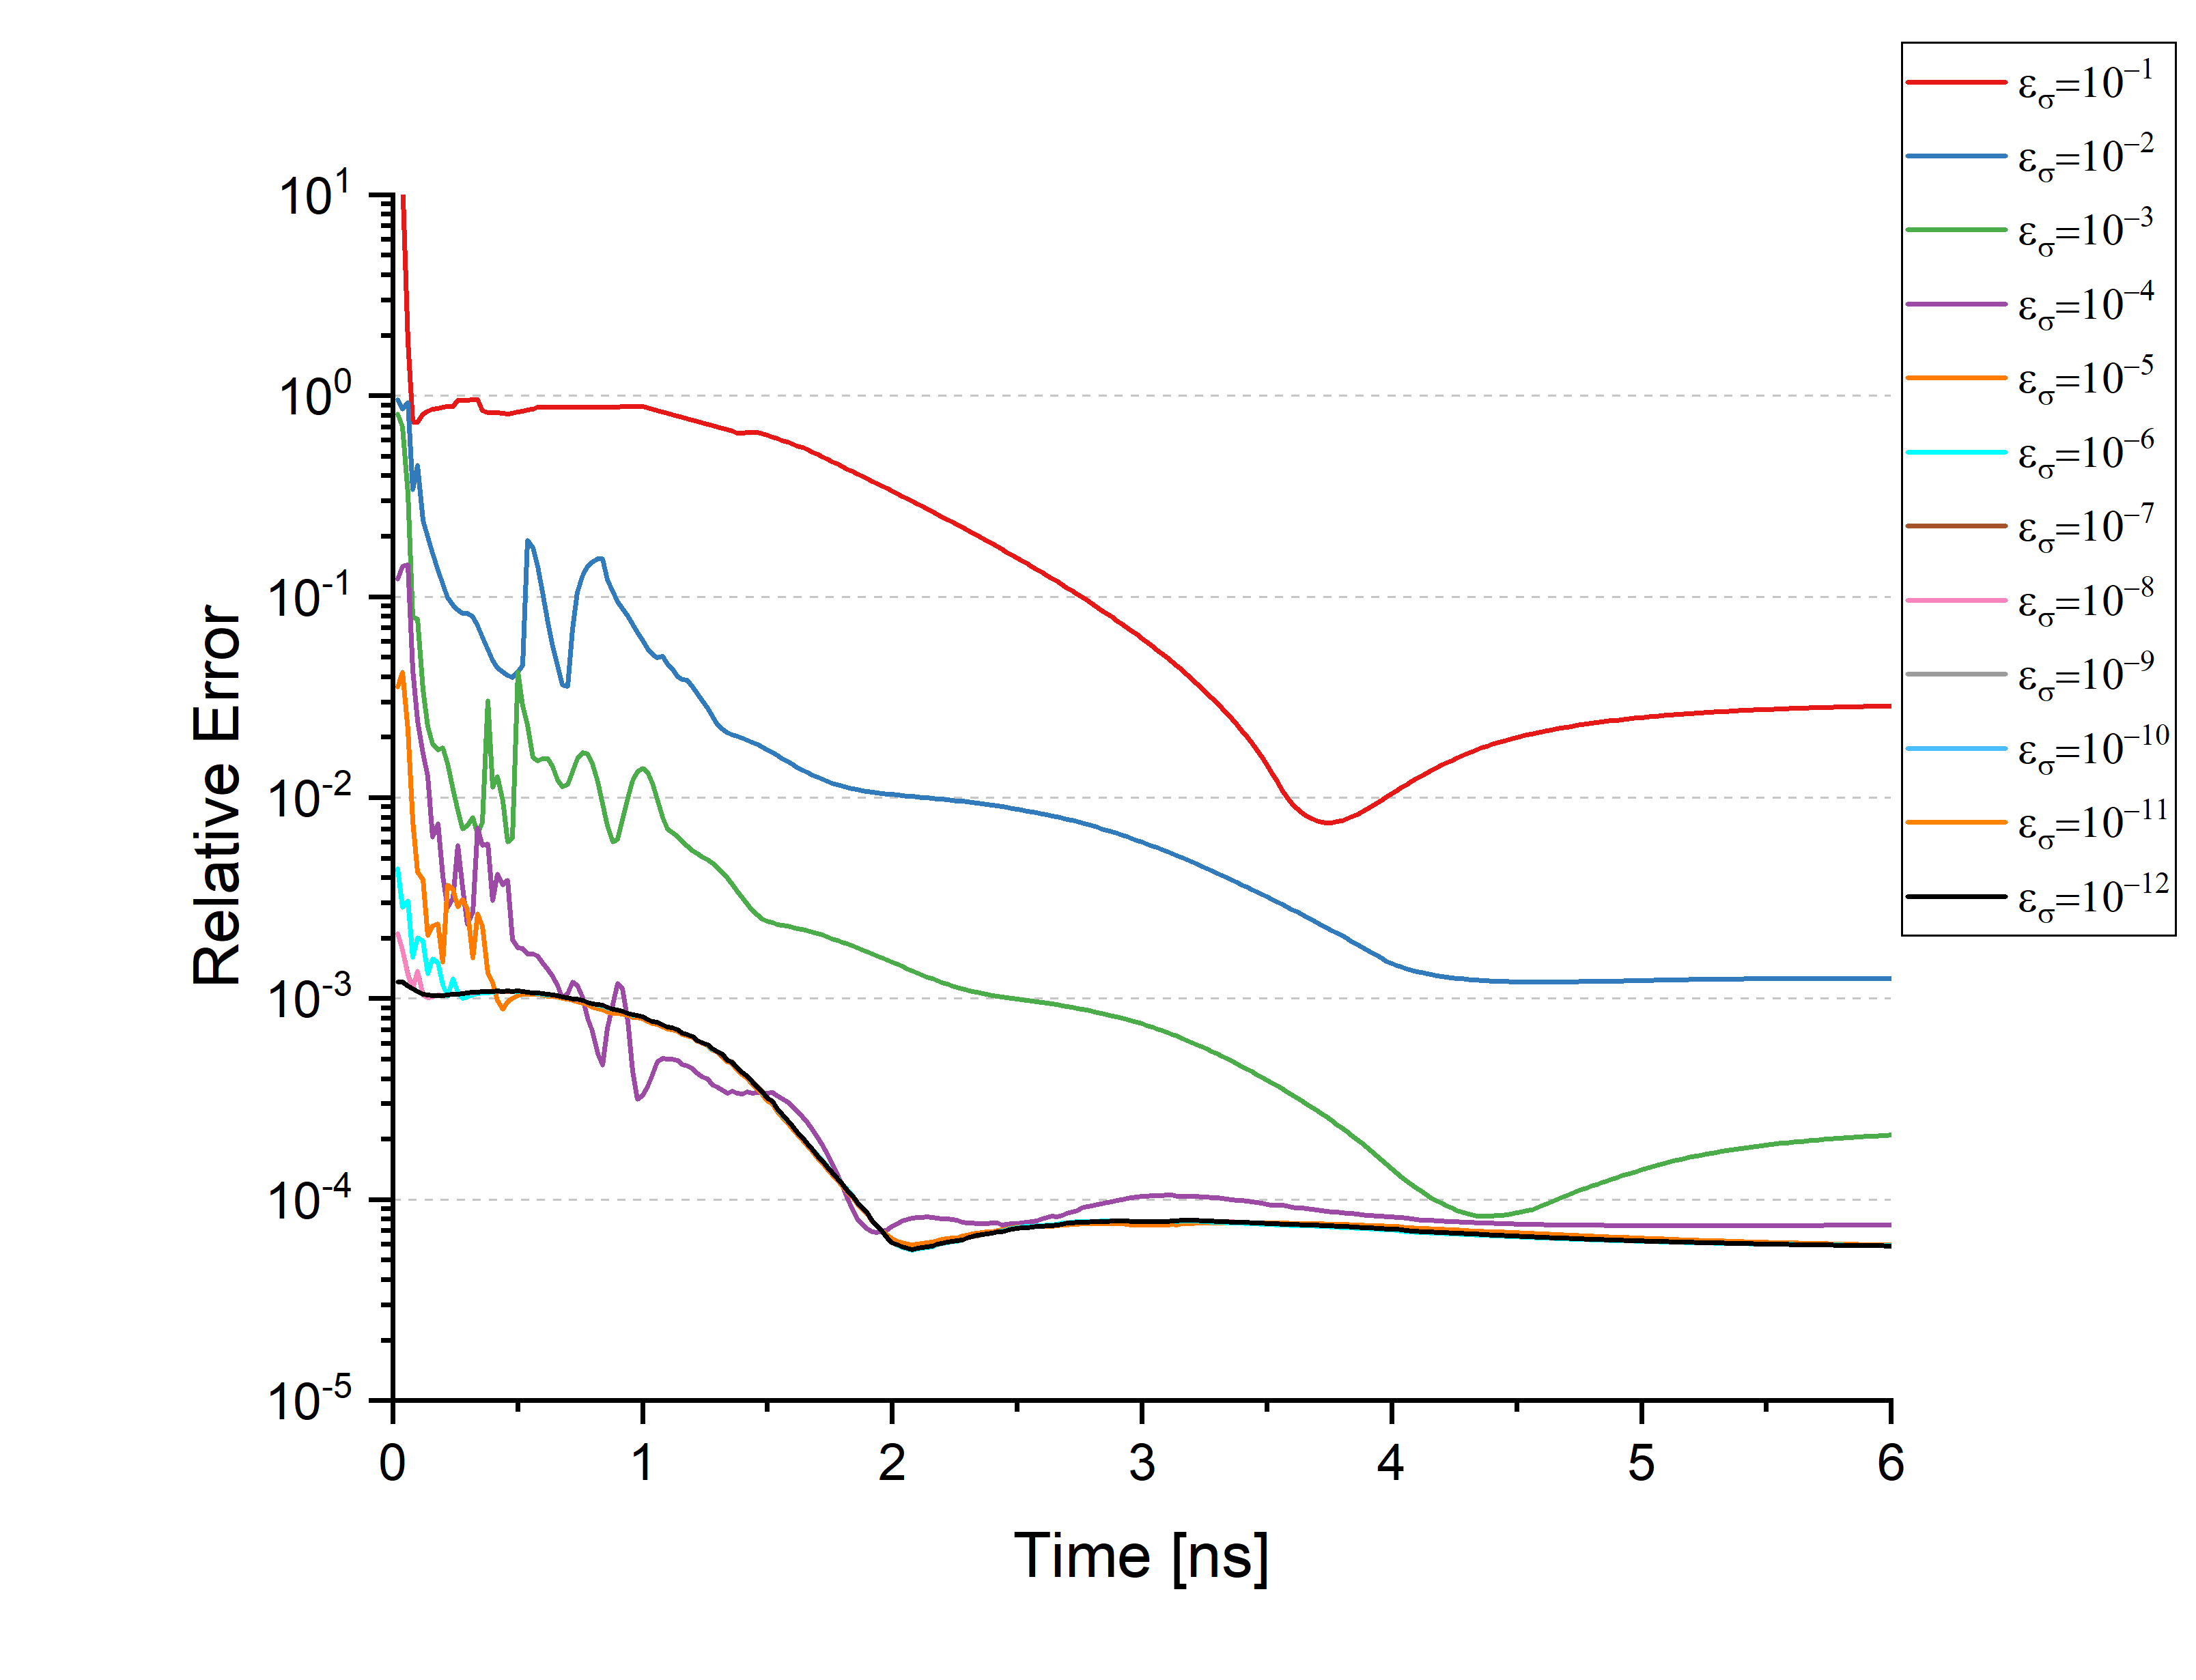
\includegraphics[width=0.475\textwidth]{GR_bc990-t002_qdf1000-980-t002_Eavg_grey_Eg_bg.png}}\\
		\subfloat[reduced rank QD factor \& energy density \newline temperature error \label{subfig:GR_bc990-t002_qdf1000-980-t002_Tavg_grey_E-fg}]{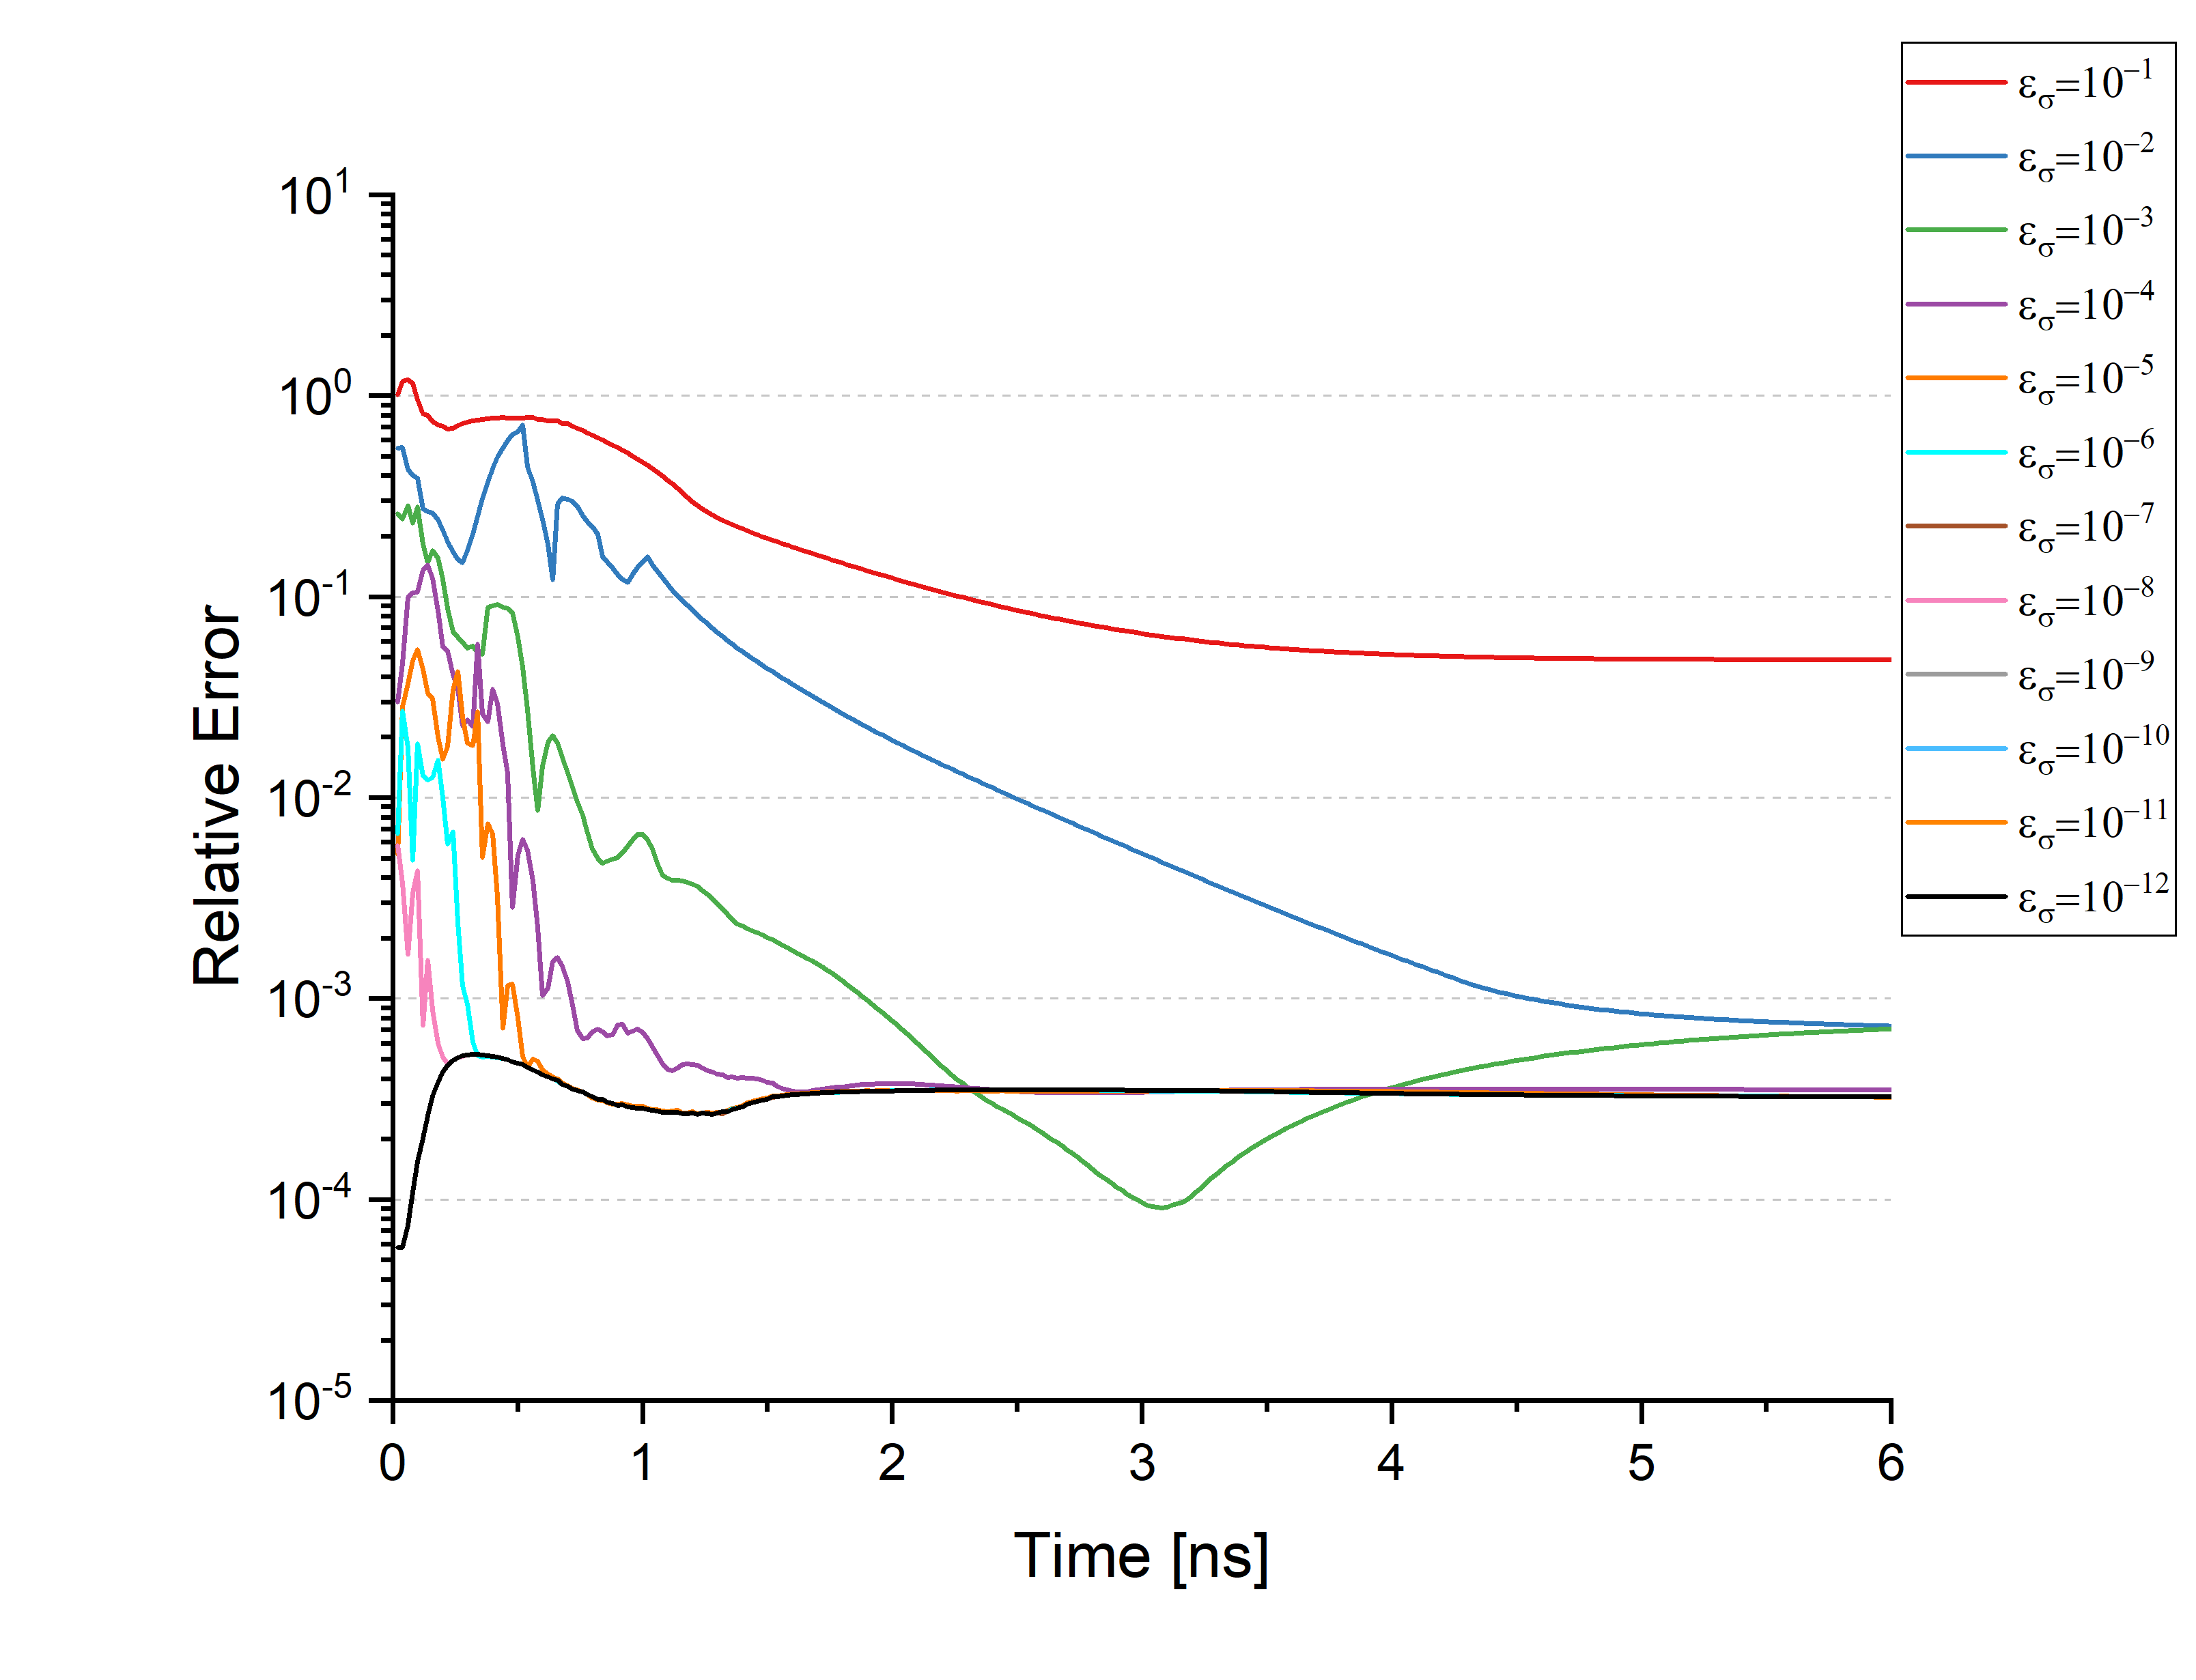
\includegraphics[width=0.475\textwidth]{GR_bc990-t002_qdf1000-980-t002_Tavg_grey_E-fg_bg}}
		\subfloat[reduced rank QD factor \& energy density total energy density error \label{subfig:GR_bc990-t002_qdf1000-980-t002_Eavg_grey_E-fg}]{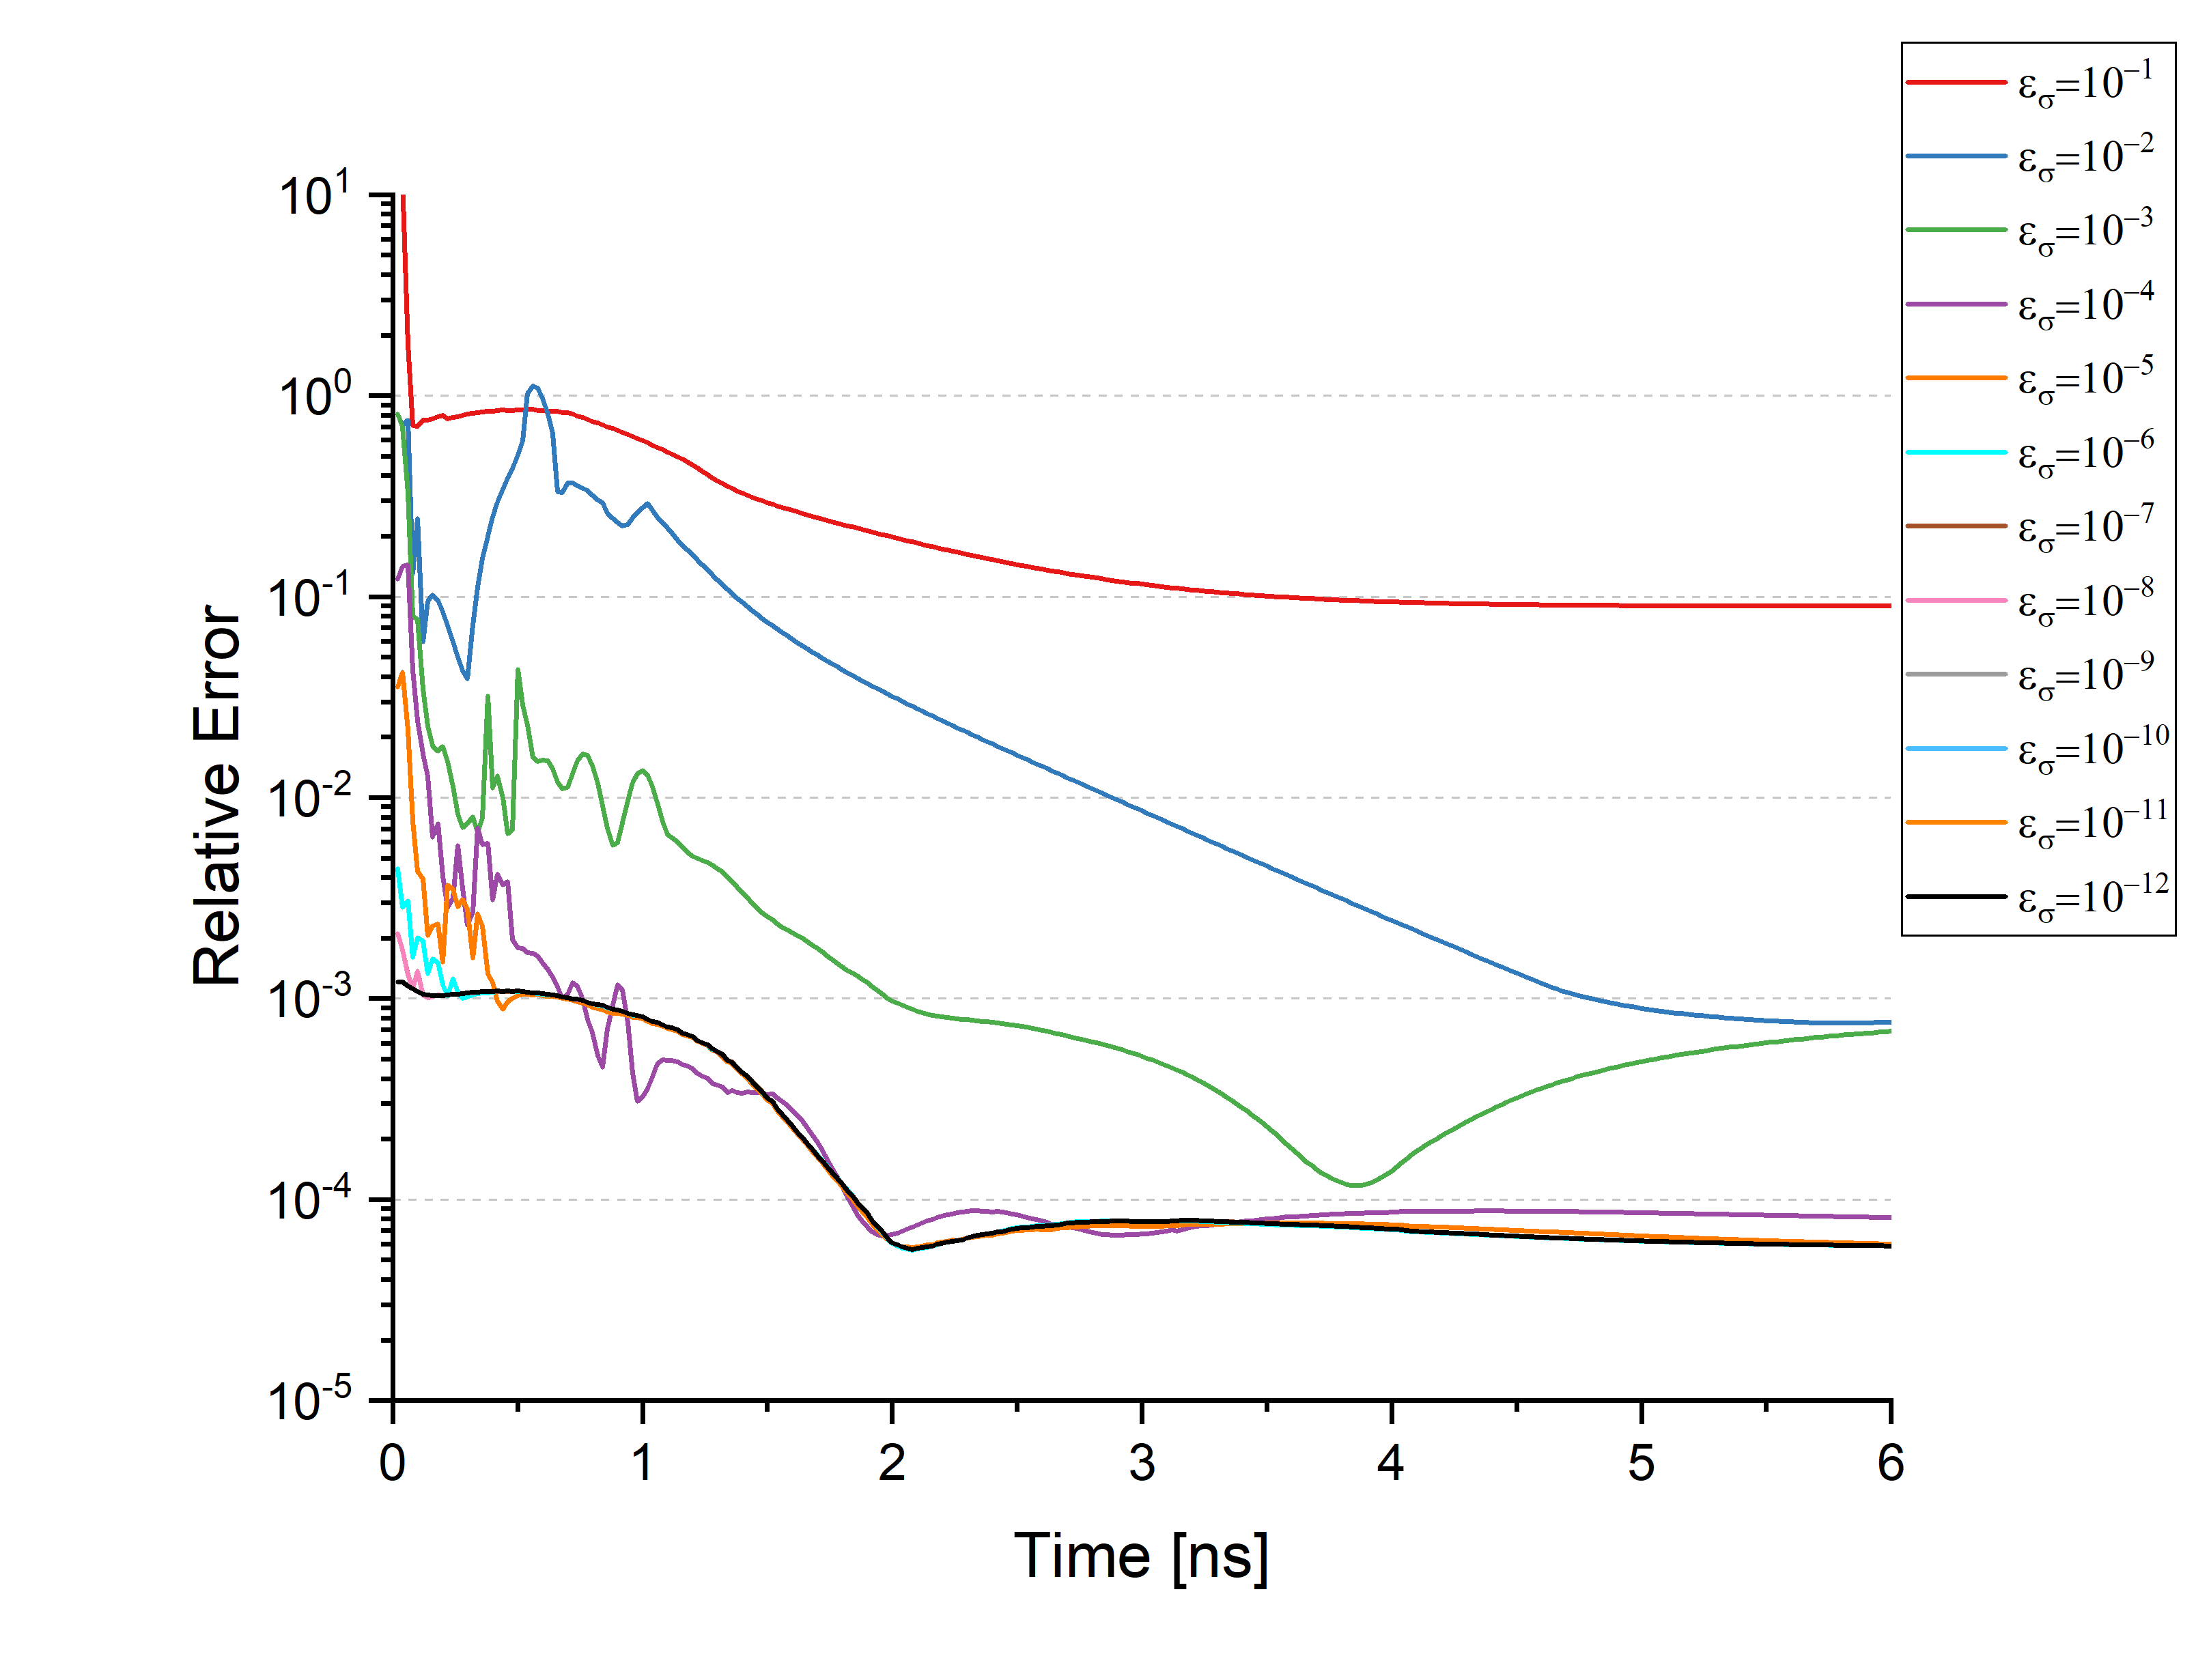
\includegraphics[width=0.475\textwidth]{GR_bc990-t002_qdf1000-980-t002_Eavg_grey_E-fg_bg}}
		\caption{\label{fig:errors_bc_T=990_grey}
			Relative error in the $L_1$-norm of the MLQD-POD GLOQD solutions computed with $T_{in}~=~0.99$~KeV using base cases with $\tilde T_{in}^{\pr{1}}=1$ KeV  and $\tilde T_{in}^{\pr{2}}=0.98$ KeV.}
	\end{figure}
	
	\begin{figure}[ht!]
		\centering
		\subfloat[reduced rank QD factor temperature error \label{subfig:GR_bc980-t002_qdf1000-960-t002_Tavg_grey_fg}]{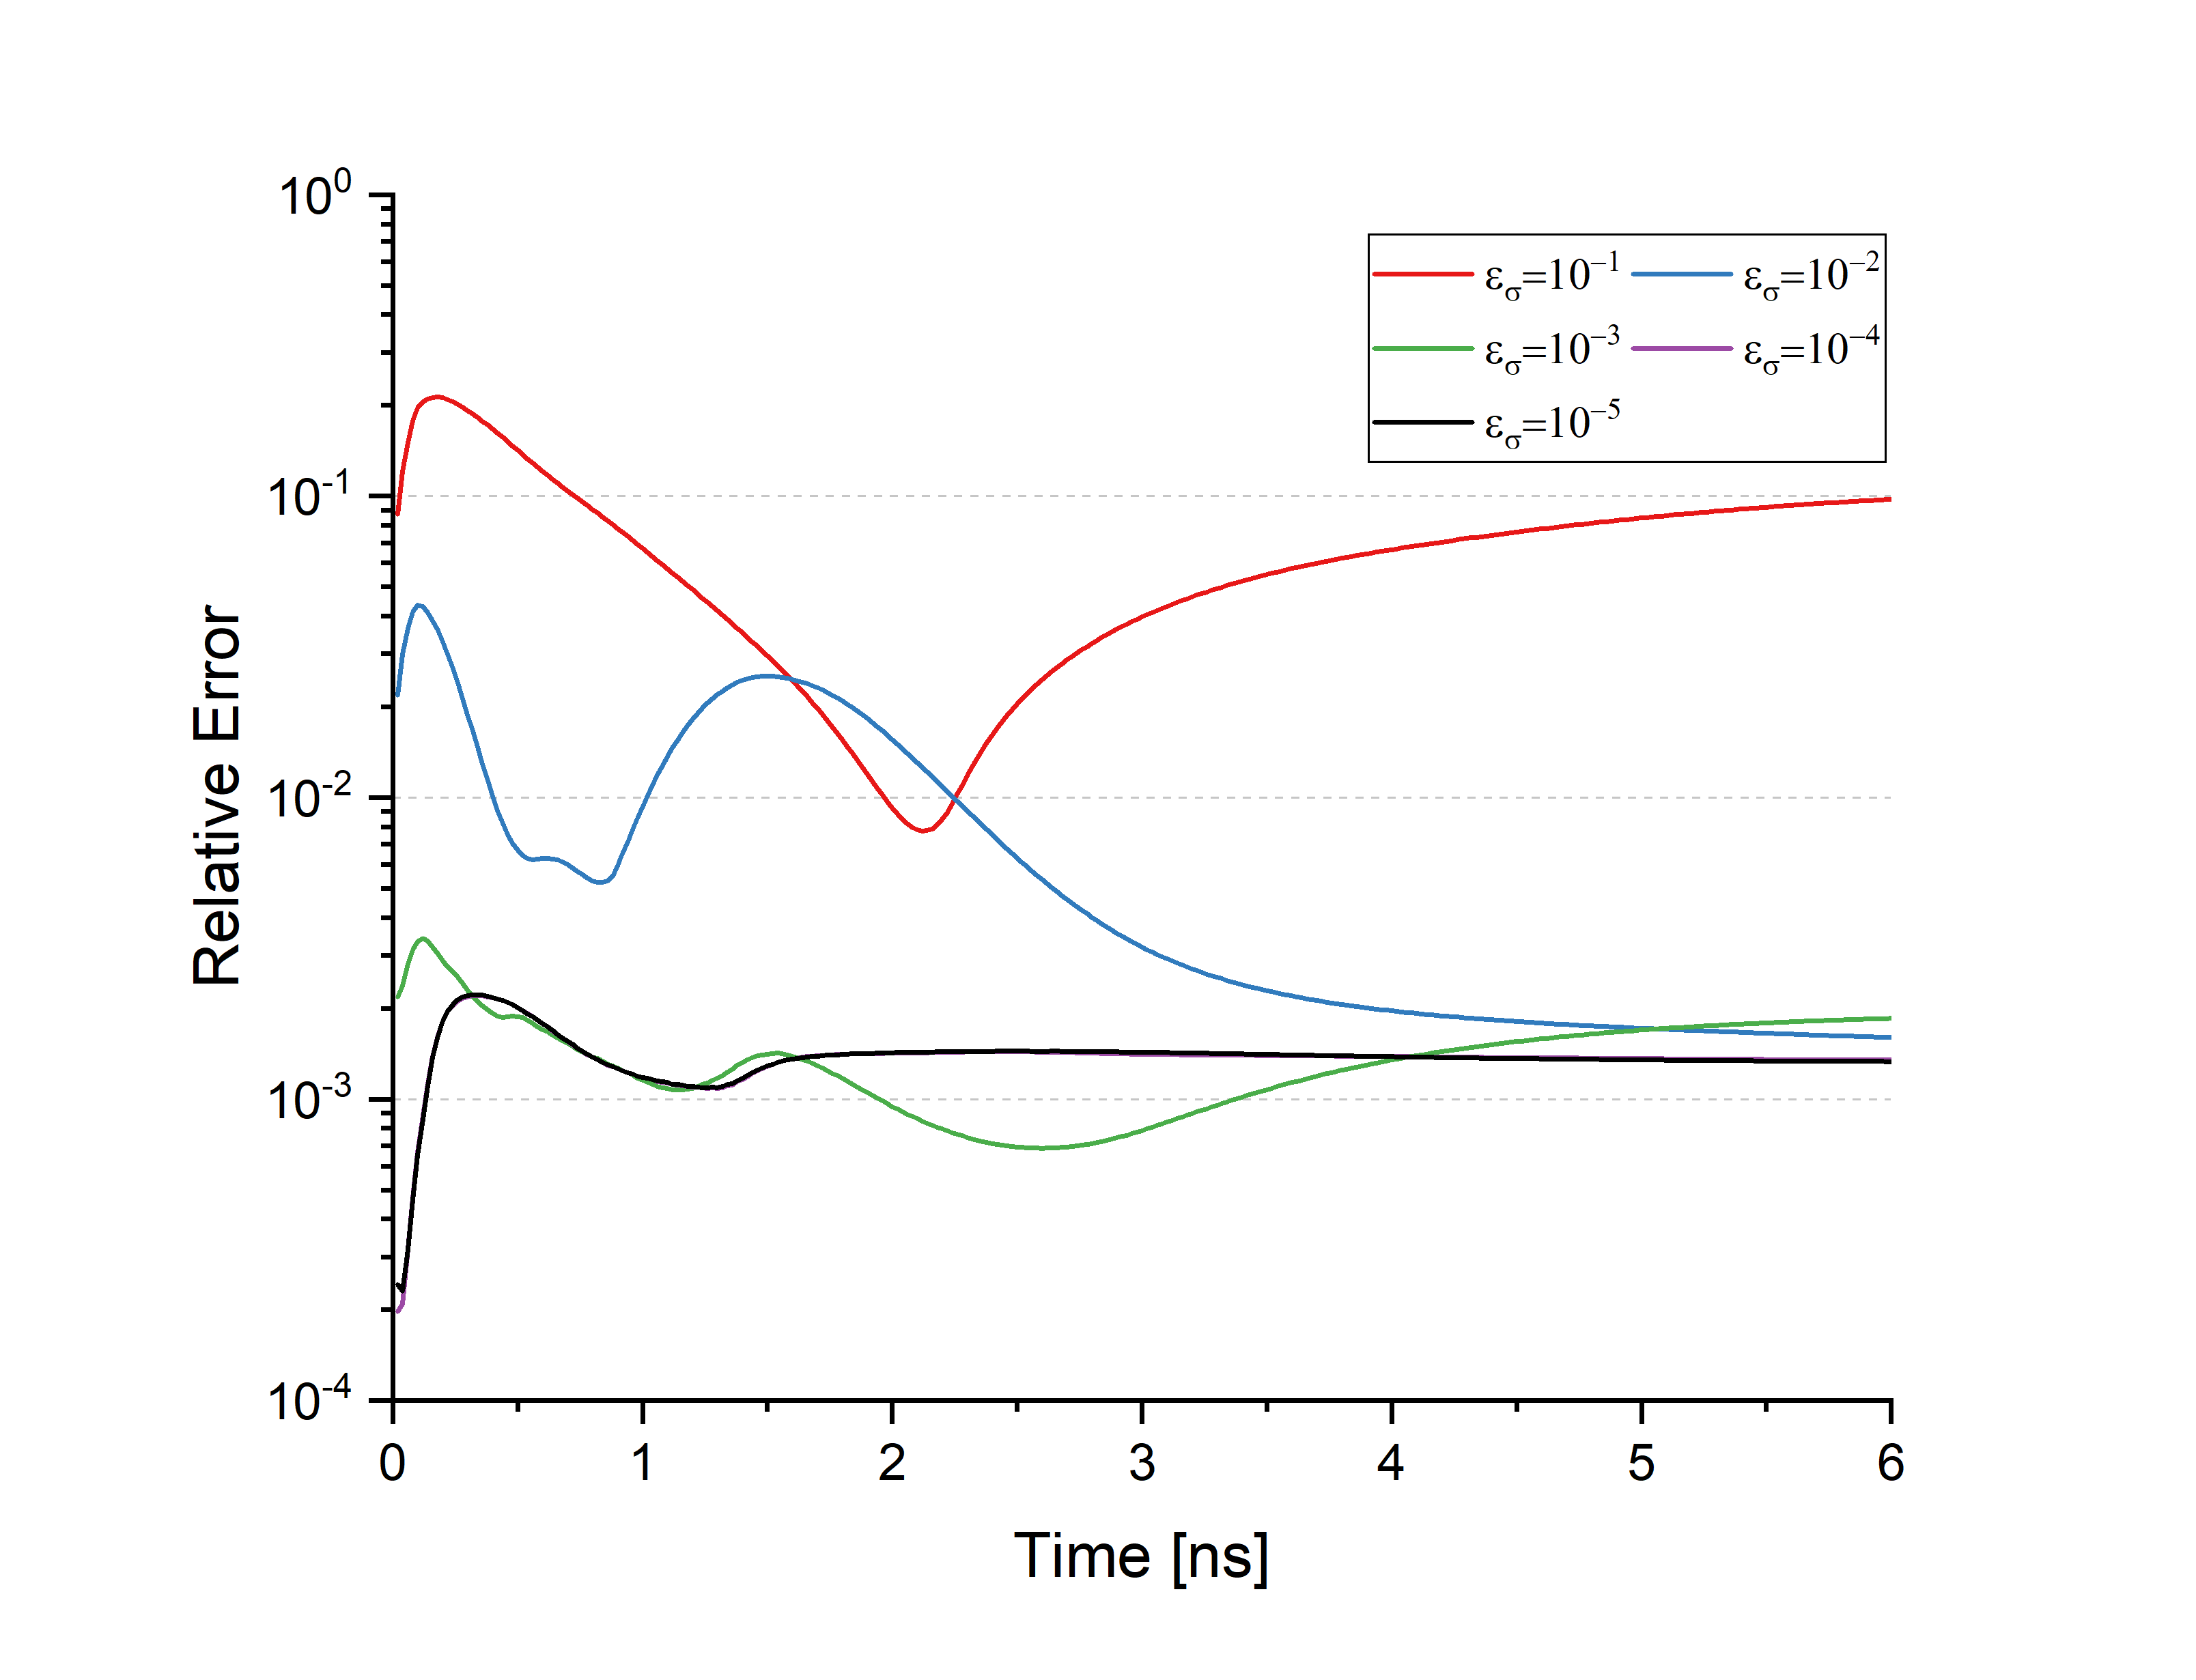
\includegraphics[width=0.475\textwidth]{GR_bc980-t002_qdf1000-960-t002_Tavg_grey_fg_bg.png}}
		\subfloat[reduced rank QD factor total energy density error \label{subfig:GR_bc980-t002_qdf1000-960-t002_Eavg_grey_fg}]{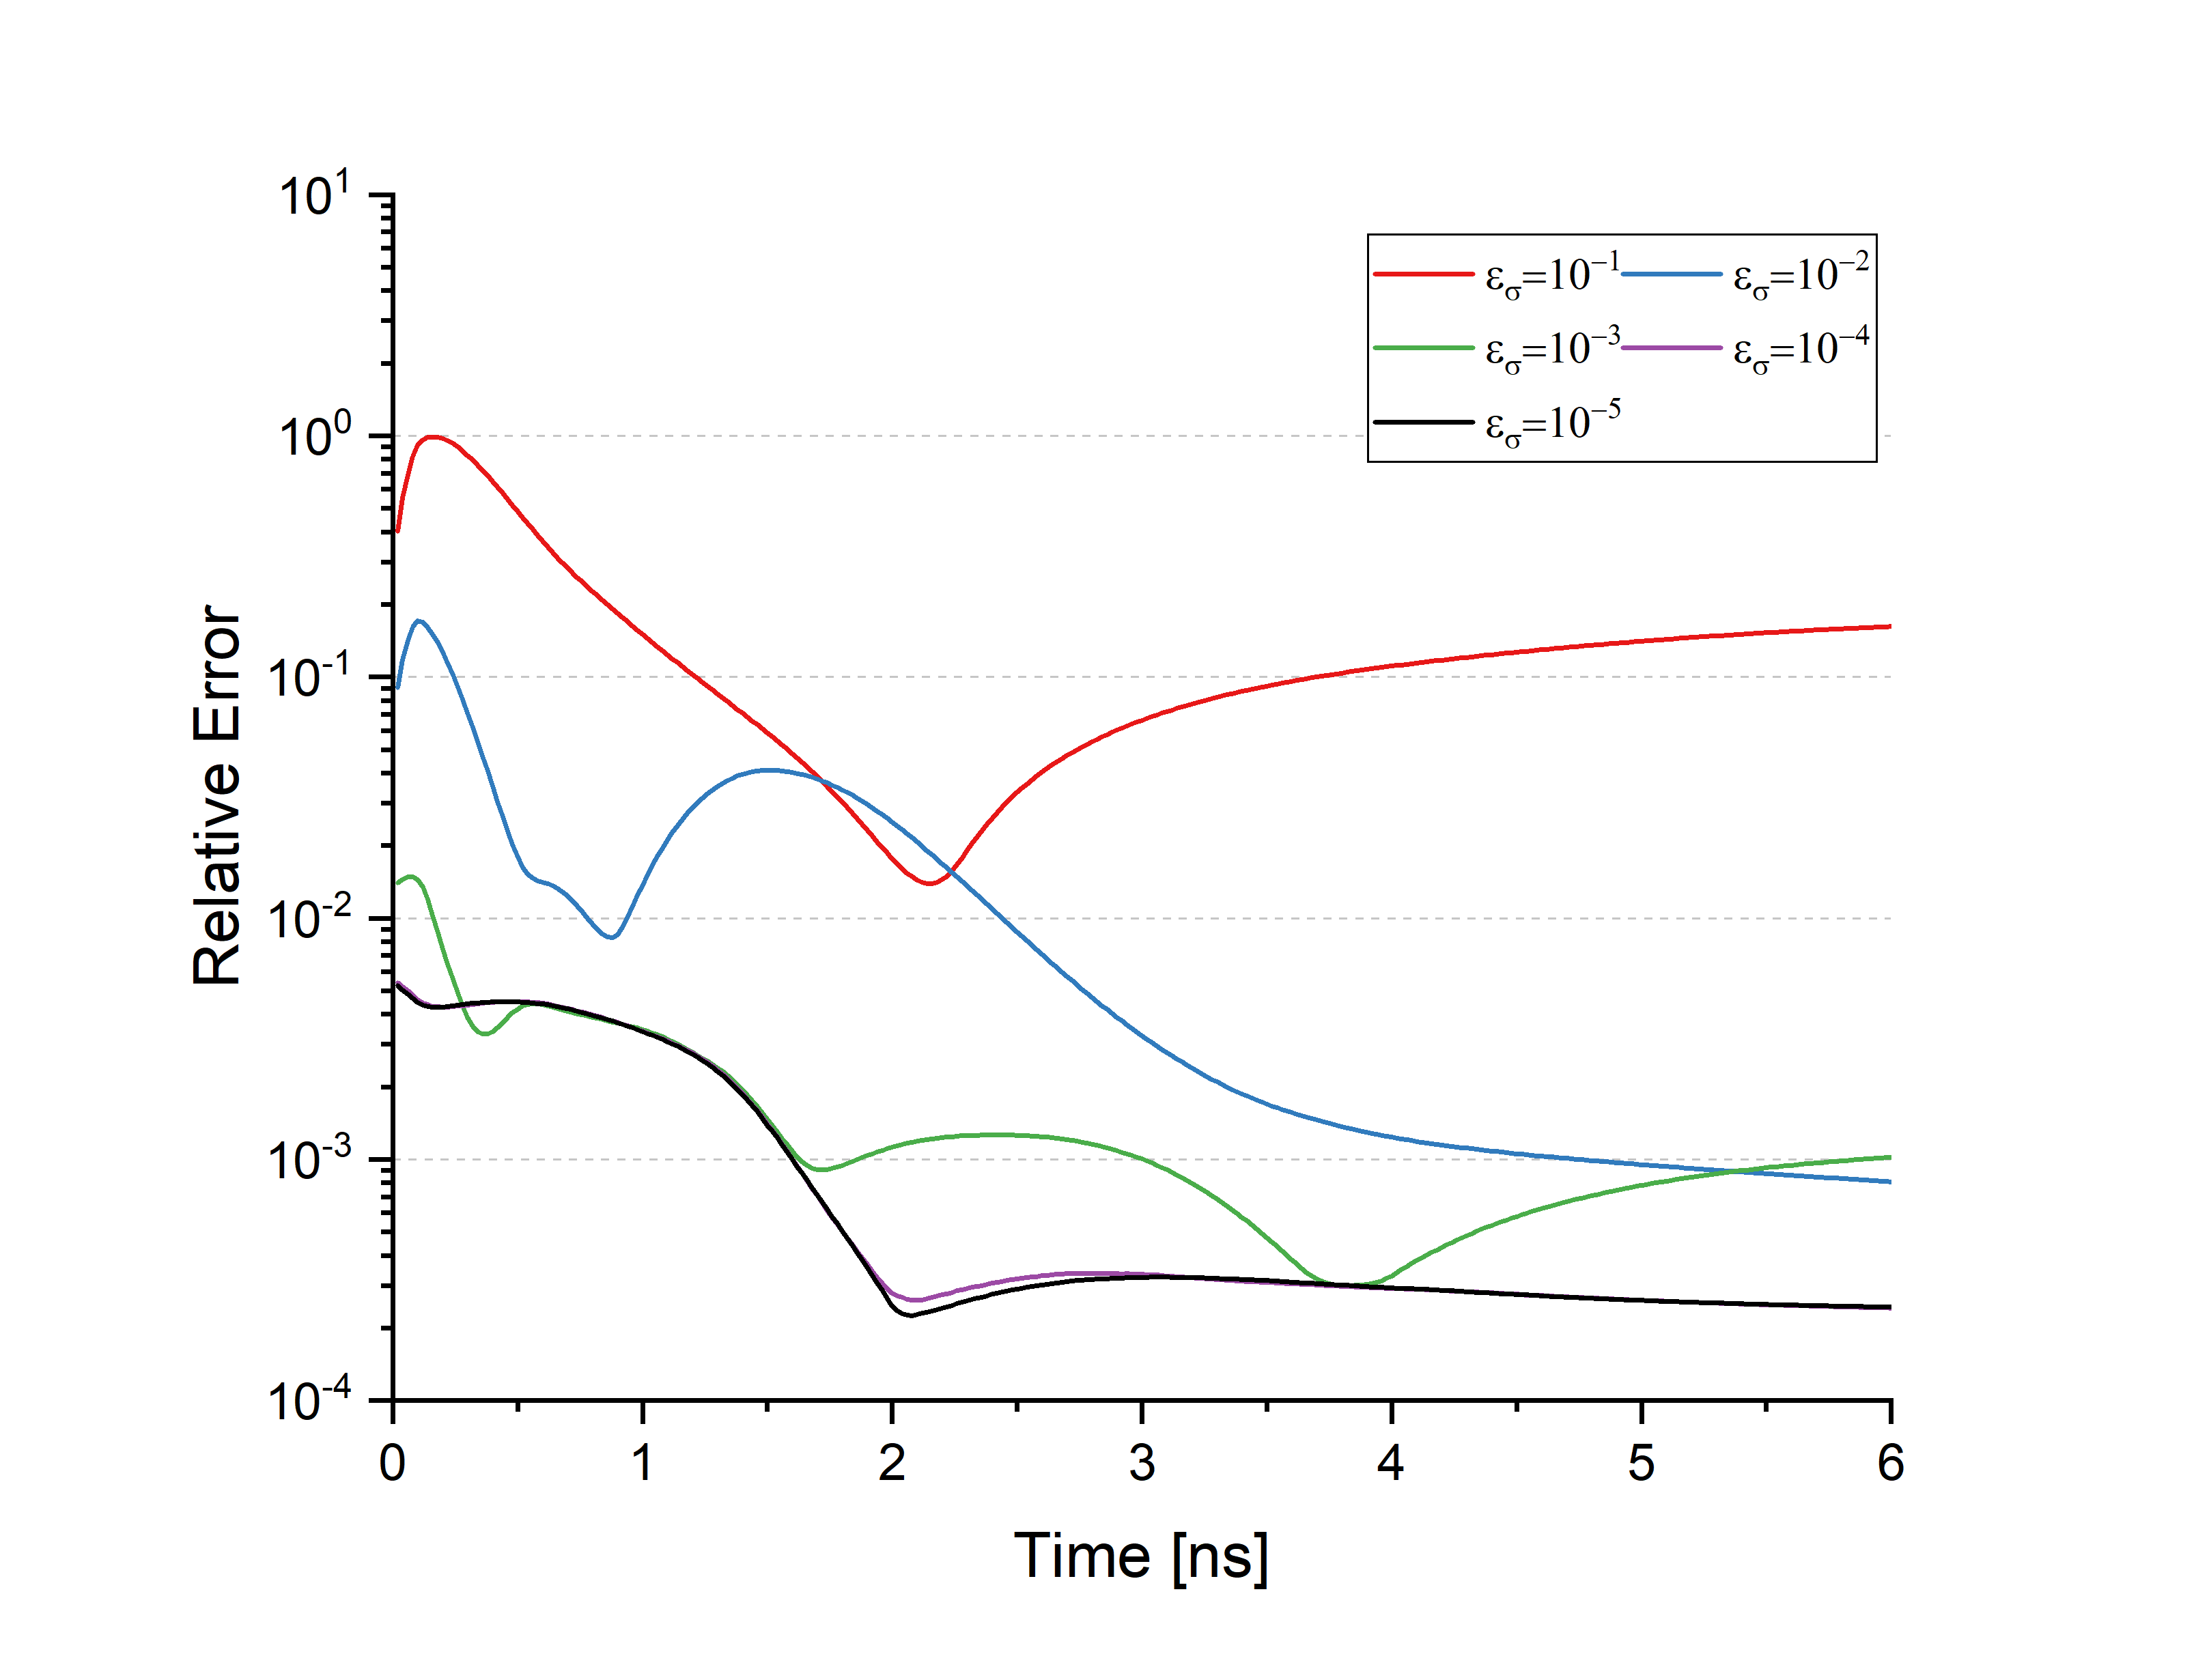
\includegraphics[width=0.475\textwidth]{GR_bc980-t002_qdf1000-960-t002_Eavg_grey_fg_bg.png}}\\
		\subfloat[reduced rank energy density temperature error \label{subfig:GR_bc980-t002_qdf1000-960-t002_Tavg_grey_Eg}]{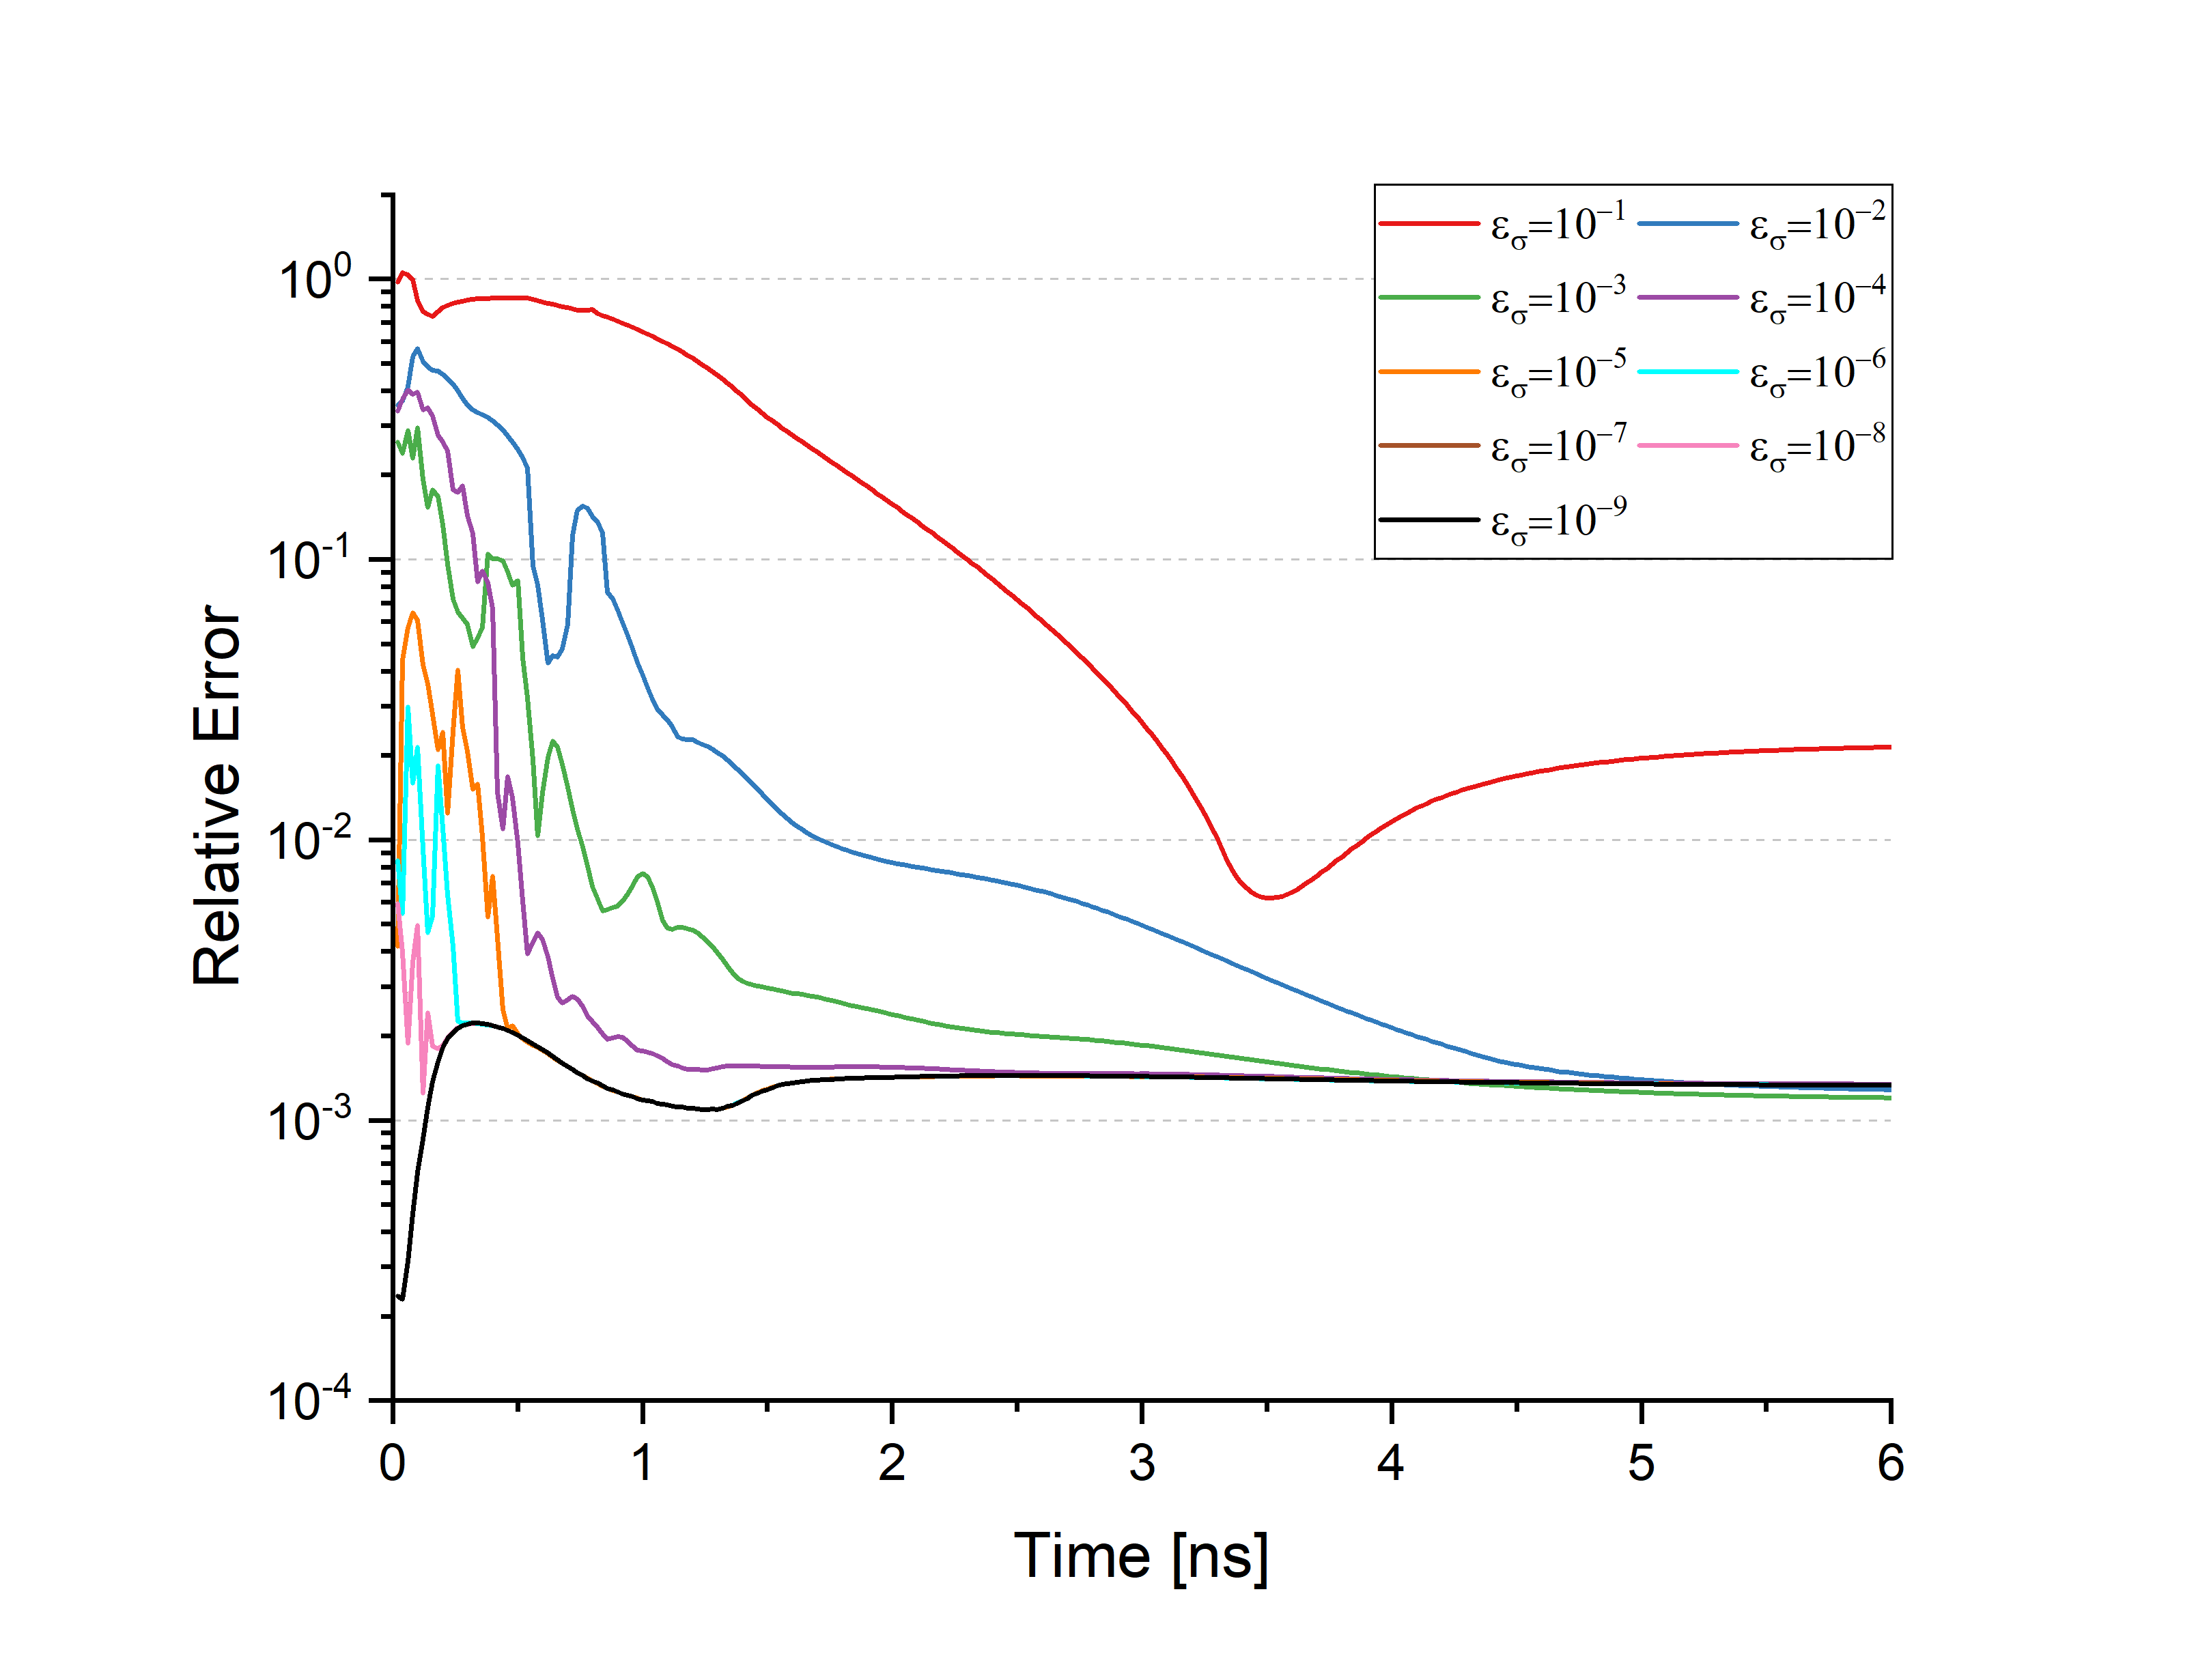
\includegraphics[width=0.475\textwidth]{GR_bc980-t002_qdf1000-960-t002_Tavg_grey_Eg_bg.png}}
		\subfloat[reduced rank energy density total energy density error \label{subfig:GR_bc980-t002_qdf1000-960-t002_Eavg_grey_Eg}]{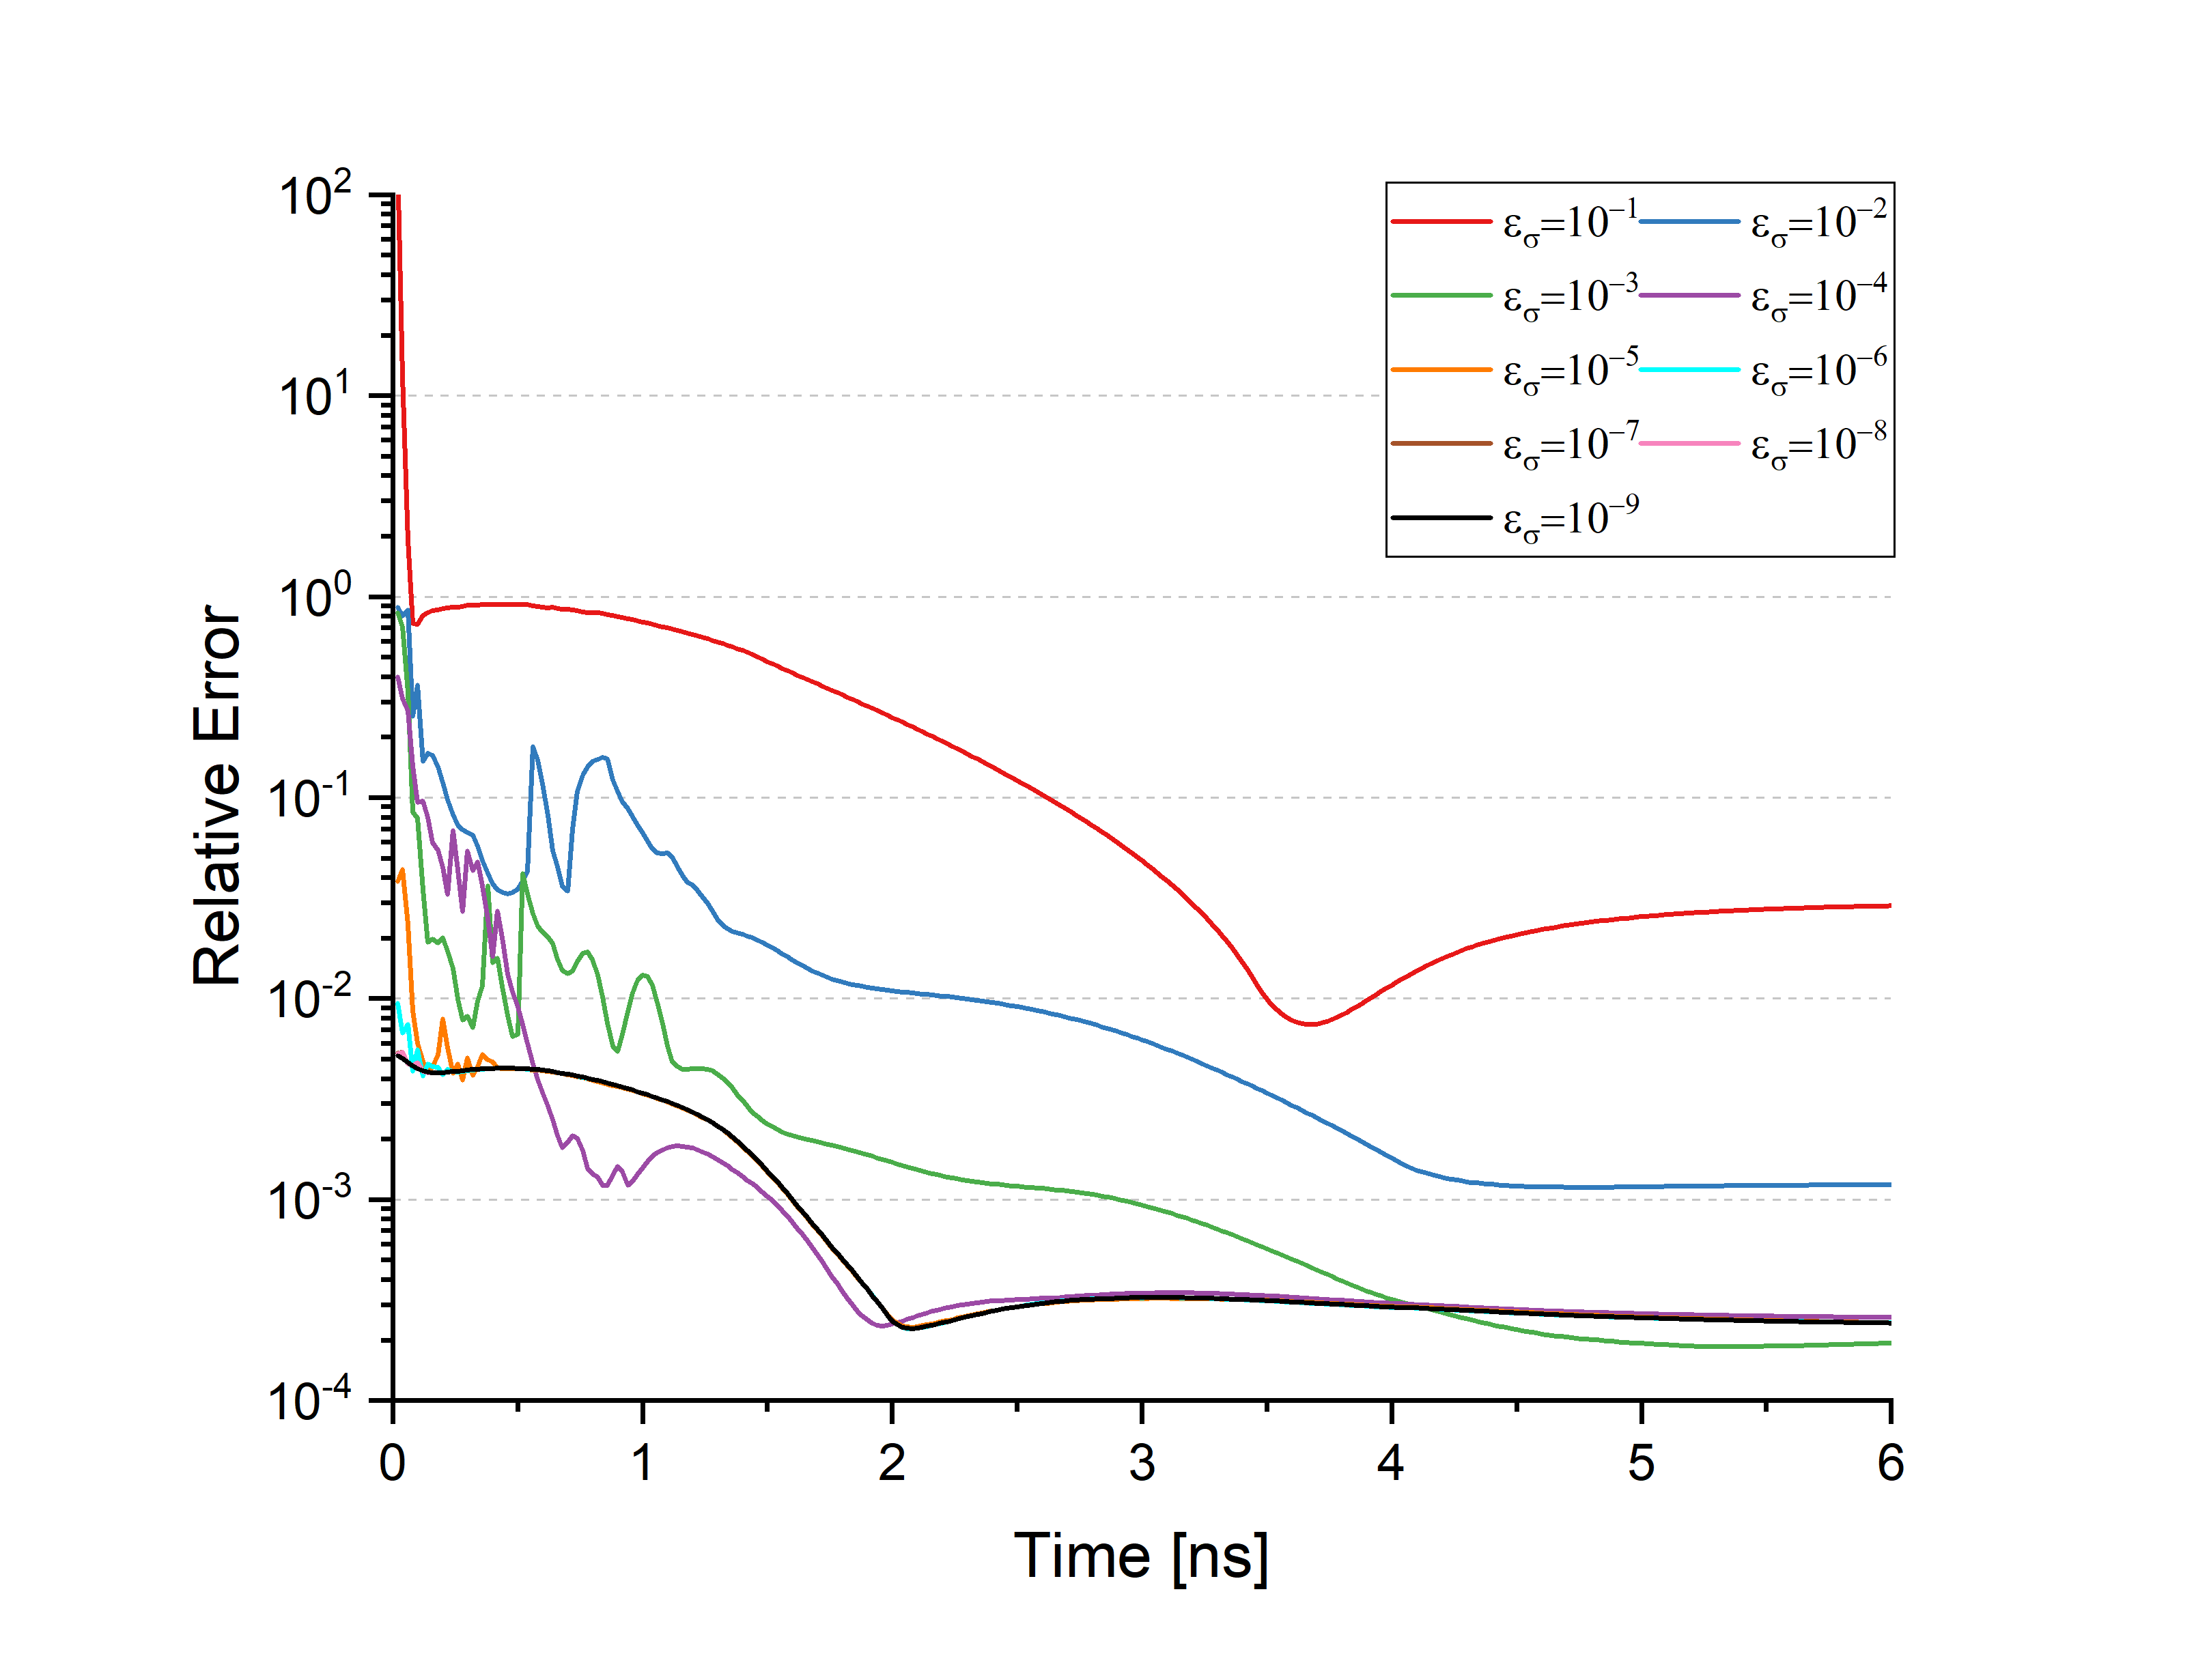
\includegraphics[width=0.475\textwidth]{GR_bc980-t002_qdf1000-960-t002_Eavg_grey_Eg_bg.png}}\\
		\subfloat[reduced rank QD factor \& energy density \newline temperature error \label{subfig:GR_bc980-t002_qdf1000-960-t002_Tavg_grey_E-fg}]{\includegraphics[width=0.475\textwidth]{GR_bc980-t002_qdf1000-960-t002_Tavg_grey_E-fg_bg}}
		\subfloat[reduced rank QD factor \& energy density total energy density error \label{subfig:GR_bc980-t002_qdf1000-960-t002_Eavg_grey_E-fg}]{\includegraphics[width=0.475\textwidth]{GR_bc980-t002_qdf1000-960-t002_Eavg_grey_E-fg_bg}}
		\caption{\label{fig:errors_bc_T=980_grey}
			Relative error in the $L_1$-norm of the MLQD-POD GLOQD solutions computed with $T_{in}~=~0.98$~KeV using base cases with $\tilde T_{in}^{\pr{1}}=1$ KeV  and $\tilde T_{in}^{\pr{2}}=0.96$ KeV.}
	\end{figure}
	
	
	%%%%%%%%%%%%%%%%%%%%%%%%%%%%%%%%%%%%%%
	% PARAMETERIZED SECTION
	\iffalse

	\ind The GLOQD-POD ROM is now extended to solve problems with an incomplete database. A simple version of this ROM is to solve the F-C test with a time step length smaller than that used to calculate the POD database. This requires the GLOQD-POD ROM to solve the F-C test for more instants of time than the database provides information for. $\bfg^*$ and $\eg^*$ for times not included in the database are calculated with linear interpolation between recorded database values. Fig. \ref{fig:errors_dt-0.01_grey} shows the  relative error in $L_1$-norm of the GLOQD-POD ROM solution computed with $\Delta t \! =  \! 1\! \times  \!  10^{-2}$ ns using various values of $\varepsilon_{\sigma}$. Fig. \ref{fig:errors_dt-0.005_grey}  presents the relative error in the solutions computed with $\Delta t \! = \! 5\! \times  \! 10^{-3}$ ns. The error for most cases saturated at $\varepsilon_\sigma = 5,6$ and so smaller $\varepsilon_\sigma$ are not shown. All cases have the most error at the early times of the problem which decreases by several orders of magnitude as the problem progresses. The cases which used reduced rank approximation of QD factors and exact energy densities had very similar errors to the cases shown for the MLOQD-POD ROM. This is to be expected as it should emulate the MLOQD-POD method since exact group energy densities are used. The saturation level error does not change significantly between cases that use the exact reference value and reduced rank forms of the group QD factors and energy densities. Note in Fig. \ref{fig:errors_dt-0.005_grey}, the error does not monotonically decrease as $\varepsilon_\sigma$ decreases. This effect is only present when using the reduced rank form of the group energy densities. The effect is different between the cases using exact and reduced rank approximation of group QD factors, but can be attributed solely to how the reduced rank approximation of group energy densities are formed as it is not observed with the exact group radiation energy densities. As described in Sec. \ref{reduced_eg} the full rank POD of the group energy densities is not equivalent to the exact reference group energy densities due to numeric limitations. This creates large errors in areas dominated by background radiation where the group energy densities are most poorly represented. In such cases where the database is especially limited, it makes sense that the black body radiation spectrum would be a more accurate representation of the group radiation energy densities in those areas than what is given by the database. For the case of $\Delta t \! = \! 5\! \times  \! 10^{-3}$ ns, the interpolated database values even for the full rank representation fall into this regime. The ROMs using large $\varepsilon_\sigma$ make more use of the black-body correction for group radiation energy densities described in Sec. \ref{bb_cor} than the ROMs using small $\varepsilon_\sigma$. Thus, the early times of the F-C problem solved using a large $\varepsilon_\sigma$ where the majority of nonlocal group radiation energy densities are approximated with the black-body spectrum can feasibly find a more accurate solution than when using small  $\varepsilon_\sigma$ with most of the nonlocal group radiation energy densities being approximated with the POD database. This is also observed to a much lesser extent in Fig. \ref{fig:errors_dt-0.01_grey}. The effect only takes on real significance for the ROM using $\Delta t \! = \! 5\! \times  \! 10^{-3}$ ns because the reduced rank database values are much more approximate than for $\Delta t \! = \! 1\! \times  \! 10^{-2}$ and limits the full rank representation of some group radiation energy densities to be less accurate than the black-body spectrum for some times.

	%%%%%%%%%%%%%%%%%%%%%%%%%%%%%%%%%%%%%%
	% PARAMETERIZED SECTION
	%\iffalse
	\ind As done for the MLOQD-POD ROM, the GLOQD-POD ROM can be extended to develop a parameterized ROM for a class of TRT problems using QD factors and radiation energy densities estimated from a set of base cases. In this study we consider a ROM parameterized with respect to the temperature $T_{in}$ of incoming radiation at the left boundary. A database of the group QD factors and radiation energy densities is formed for problems with two selected temperatures of incoming radiation  $T_{in}^{(1)}$ and $T_{in}^{(2)}$. The GLOQD-POD ROM solutions of TRT problems with incoming radiation at some given temperature are calculated using the group QD factors and radiation energy densities obtained by linear interpolation between values in the database. Results are presented for three parametrized ROMs. One model uses $T_{in}^{(1)}~=~1$~KeV and $T_{in}^{(2)}=0.98$ KeV. The second one is formed with  $T_{in}^{(1)}=1$ KeV and $T_{in}^{(2)}=0.96$ KeV. The third is formed with  $T_{in}^{(1)}=1$ KeV and $T_{in}^{(2)}=0.92$ KeV. The data is generated for $\Delta t = 2\times10^{-2}$ ns. Fig. \ref{fig:errors_bc_T=990_grey} shows the relative error in $L_1$-norm in the solution for $T_{in}=0.99$ KeV computed by means of first parametrized GLOQD-POD ROM with various values of $\varepsilon_{\sigma}$. Fig. \ref{fig:errors_bc_T=980_grey} presents the relative error of the GLOQD-POD ROM solution  for $T_{in}= 0.98$ KeV obtained from the second model that is parametrized with a larger interval of  $[T_{in}^{(1)},T_{in}^{(2)}]$. Fig. \ref{fig:errors_bc_T=960} presents the relative error of the MLOQD-POD ROM solution  for $T_{in}= 0.96$ KeV obtained from the third model that is parameterized with the largest interval of  $[T_{in}^{(1)},T_{in}^{(2)}]$. The reference MLQD solution is computed for each value of $T_{in}$ to obtain relative errors.
	
	\ind The error for most cases saturated at $10^{-5} \leq \varepsilon_\sigma \leq 10^{-9}$ and so smaller $\varepsilon_\sigma$ are not shown. The cases which used reduced rank QD factors and exact energy densities had very similar errors to the cases shown for the MLOQD-POD ROM for the same parameterization in $T_{in}$. The saturated error for using only reduced rank QD factors, only energy densities or both in reduced rank form is similar in magnitude and shape. The saturated error for all cases increases as the interval of  $[T_{in}^{(1)},T_{in}^{(2)}]$ is increased, seeing roughly a 5 times increase between $T_{in}= 0.99$ KeV and $T_{in}= 0.98$ KeV. The effect causing large $\varepsilon_\sigma$ to be more accurate than small $\varepsilon_\sigma$ is not significantly present for any of these ROMs. Even though the largest interval of $[T_{in}^{(1)},T_{in}^{(2)}]$ is $0.8$ KeV, the reduced rank radiation energy densities remain more accurate for small $\varepsilon_\sigma$ than the black-body spectrum largely used to correct large $\varepsilon_\sigma$ cases. The error is more uniform across all times than is seen for the reduced time step ROMs, although for most cases the error is highest at the early times of the problem. When using reduced rank group radiation energy densities, smaller values of $\varepsilon_\sigma$ are required to reach the saturated error compared to when using the exact reference radiation energy densities.

	\begin{figure}[ht!]
		\centering
		\subfloat[reduced rank QD factor temperature error \label{subfig:GR_bc960-t002_qdf1000-920-t002_Tavg_grey_fg}]{\includegraphics[width=0.475\textwidth]{GR_bc960-t002_qdf1000-920-t002_Tavg_grey_fg_bg.png}}
		\subfloat[reduced rank QD factor total energy density error \label{subfig:GR_bc960-t002_qdf1000-920-t002_Eavg_grey_fg}]{\includegraphics[width=0.475\textwidth]{GR_bc960-t002_qdf1000-920-t002_Eavg_grey_fg_bg.png}}\\
		\subfloat[reduced rank energy density temperature error \label{subfig:GR_bc960-t002_qdf1000-920-t002_Tavg_grey_Eg}]{\includegraphics[width=0.475\textwidth]{GR_bc960-t002_qdf1000-920-t002_Tavg_grey_Eg_bg.png}}
		\subfloat[reduced rank energy density total energy density error \label{subfig:GR_bc960-t002_qdf1000-920-t002_Eavg_grey_Eg}]{\includegraphics[width=0.475\textwidth]{GR_bc960-t002_qdf1000-920-t002_Eavg_grey_Eg_bg.png}}\\
		\subfloat[reduced rank QD factor \& energy density temperature error \label{subfig:GR_bc960-t002_qdf1000-920-t002_Tavg_grey_E-fg}]{\includegraphics[width=0.475\textwidth]{GR_bc960-t002_qdf1000-920-t002_Tavg_grey_E-fg_bg}}
		\subfloat[reduced rank QD factor \& energy density total energy density error \label{subfig:GR_bc960-t002_qdf1000-920-t002_Eavg_grey_E-fg}]{\includegraphics[width=0.475\textwidth]{GR_bc980-t002_qdf1000-960-t002_Eavg_grey_E-fg_bg}}
		\caption{\label{fig:errors_bc_T=960_grey}
			Relative error in the $L_1$-norm of the MLQD-POD GLOQD solutions computed with $T_{in}~=~0.96$~KeV using base cases with $\tilde T_{in}^{\pr{1}}=1$ KeV  and $\tilde T_{in}^{\pr{2}}=0.92$ KeV.}
	\end{figure}

	\fi
	%%%%%%%%%%%%%%%%%%%%%%%%%%%%%%%%%%%%%%